\pdfoutput=1

\documentclass[11pt]{article}

\newif\ifreviewcopy
\reviewcopyfalse

\usepackage{acl}
\usepackage{times}
\usepackage{latexsym}
\usepackage[T1]{fontenc}
\usepackage[utf8]{inputenc}
\usepackage{microtype}
\usepackage[colorinlistoftodos]{todonotes}
\usepackage{marginnote}
\usepackage{amsmath}
\usepackage{enumitem}
\usepackage{placeins}
\usepackage{multicol}
\usepackage{booktabs}
\usepackage[inkscapearea=page]{svg}
\usepackage{amsmath}
\usepackage[nameinlink]{cleveref}
\usepackage{float}
\usepackage{afterpage}
\usepackage{pgfplots}
\usepackage{graphicx}
\usepackage{ulem}
\usepackage[multiple,hang,flushmargin]{footmisc}
\usepackage{multirow}
\usepackage{multicol}
\usepackage{makecell}
\usepackage{mathtools}
\usepackage{amssymb}
\usepackage{pifont}
\usepackage{xspace}
\usepackage{csquotes}
\usepackage{tabularx}
\usepackage{algorithmicx}
\usepackage{algorithm}
\usepackage{algpseudocode}

\usepackage{listings}
\usepackage{xcolor}

\definecolor{codegreen}{rgb}{0,0.6,0}
\definecolor{codegray}{rgb}{0.5,0.5,0.5}
\definecolor{codepurple}{rgb}{0.58,0,0.82}
\definecolor{backcolour}{rgb}{0.95,0.95,0.92}

\lstdefinelanguage{SPARQL}{
  morekeywords=[1]{SELECT, WHERE, FILTER, OPTIONAL, UNION, GRAPH, LIMIT, OFFSET},
  morekeywords=[2]{rdf:type},
  morekeywords=[3]{xsd:integer},
  morestring=[b][\color{blue}]",
  sensitive=false,
  morecomment=[l][\color{codegreen}]{\#},
  morecomment=[s][\color{codegreen}]{/*}{*/},
}


\newcommand{\sparqlbasicstyle}{\small\ttfamily}

\lstdefinestyle{sparqlstyle}{
  backgroundcolor=\color{backcolour},
  commentstyle=\color{codegreen},
  keywordstyle=[1]\color{blue},
  keywordstyle=[2]\color{codepurple},
  keywordstyle=[3]\color{orange},
  numberstyle=\tiny\color{codegray},
  basicstyle=\sparqlbasicstyle,
  breakatwhitespace=false,
  breaklines=true,
  captionpos=b,
  keepspaces=true,
  numbers=left,
  numbersep=5pt,
  showspaces=false,
  showstringspaces=false,
  showtabs=false,
  tabsize=2,
  extendedchars=true,
  inputencoding=utf8,
  literate={á}{{\'a}}1 {ã}{{\~a}}1 {é}{{\'e}}1 {β}{{$\beta$}}1 {–}{{-}}1 {≤}{{$\leq$}}1 {≥}{{$\geq$}}1 {’}{{'}}1 {‘}{{'}}1,
  xleftmargin=2em
}

\lstdefinelanguage{markdown}{
  basicstyle={\small\ttfamily},
  breaklines=true,
  morekeywords={},
  keywordstyle=\bfseries,
  morestring=[b]",
  stringstyle=\itshape,
  morecomment=[l][\color{blue}]{\#},
  identifierstyle=\bfseries,
  sensitive=false,
}

\lstdefinestyle{markdownstyle}{
  backgroundcolor=\color{backcolour},
  commentstyle=\color{codegreen},
  keywordstyle=[1]\color{blue},
  keywordstyle=[2]\color{codepurple},
  keywordstyle=[3]\color{orange},
  numberstyle=\tiny\color{codegray},
  basicstyle={\small\ttfamily},
  breakatwhitespace=false,
  breaklines=true,
  captionpos=b,
  keepspaces=true,
  numbers=left,
  numbersep=5pt,
  showspaces=false,
  showstringspaces=false,
  showtabs=false,
  tabsize=2,
  xleftmargin=2em
}

\newcommand{\sref}[1]{Sec.~\ref{#1}}
\newcommand{\aref}[1]{Appendix~\ref{#1}}
\newcommand{\srefplural}[1]{Sections~\ref{#1}}
\newcommand{\srefshort}[1]{\ref{#1}}
\newcommand{\tref}[1]{Table~\ref{#1}}
\newcommand{\fref}[1]{Figure~\ref{#1}}

\renewcommand{\vec}[1]{\mathbf{#1}}



\setlist[description]{leftmargin=\parindent,itemsep=0mm,labelindent=0pt,topsep=0pt,partopsep=0ex,parsep=0ex}


\definecolor{anne}{rgb}{0,0.5,0.9}
\definecolor{valentin}{rgb}{0.998,0.722,0.635}
\definecolor{anna}{rgb}{0,0.5,0.9}
\definecolor{simon}{rgb}{0.998,0.722,0.635}

\definecolor{darkgreen}{rgb}{0.0, 0.5, 0.0}

\ifreviewcopy
    \paperwidth=\dimexpr \paperwidth + 20cm\relax
    \oddsidemargin=\dimexpr\oddsidemargin + 10cm\relax
    \evensidemargin=\dimexpr\evensidemargin + 10cm\relax
    \marginparsep=2.5cm
    \marginparwidth=\dimexpr \marginparwidth + 10cm - \marginparsep\relax

    \newcommand{\valentintodo}[2][valentin]{\todo[color=#1,size=\footnotesize]{\textbf{VK:} #2}}
    \newcommand{\annetodo}[2][anne!30]{\todo[color=#1,size=\footnotesize]{\textbf{AF:} #2}}
    \newcommand{\annatodo}[2][anna]{\todo[color=#1,size=\footnotesize]{\textbf{AH:} #2}}
    \newcommand{\simontodo}[2][simon!30]{\todo[color=#1,size=\footnotesize]{\textbf{SR:} #2}}

    \newcommand{\valentintodofigure}[2][0cm]{\marginnote{\todo[color=valentin,size=\footnotesize,inline]{\textbf{VK:} #2}}[#1] }
    \newcommand{\annetodofigure}[2][0cm]{\marginnote{\todo[color=anne!30,size=\footnotesize,inline]{\textbf{AF:} #2}}[#1] }
    \newcommand{\annatodofigure}[2][0cm]{\marginnote{\todo[color=anna,size=\footnotesize,inline]{\textbf{AH:} #2}}[#1] }
    \newcommand{\simontodofigure}[2][0cm]{\marginnote{\todo[color=simon!30,size=\footnotesize,inline]{\textbf{SR:} #2}}[#1] }

    \newcommand{\red}[1]{\textcolor{red}{#1}}
    \newcommand{\blue}[1]{\textcolor{blue}{#1}}
    \newcommand{\green}[1]{\textcolor{ForestGreen}{#1}}
    \newcommand{\purple}[1]{\textcolor{purple}{#1}}

\else
    \newcommand{\valentintodo}[2][valentin]{}
    \newcommand{\annetodo}[2][anne!30]{}
    \newcommand{\annatodo}[2][anna]{}
    \newcommand{\simontodo}[2][simon!30]{}

    \newcommand{\valentintodofigure}[2][0cm]{}
    \newcommand{\annetodofigure}[2][anne!30]{}
    \newcommand{\annatodofigure}[2][anna]{}
    \newcommand{\simontodofigure}[2][simon!30]{}

    \newcommand{\red}[1]{#1}
    \newcommand{\blue}[1]{#1}
    \newcommand{\green}[1]{#1}
    \newcommand{\purple}[1]{#1}
\fi




\def\mathdefault#1{#1}

\pgfplotsset{compat=1.16}




\def\DatasetNameTitle{Pap2Pat\xspace}
\def\DatasetName{{\sc{\DatasetNameTitle}}\xspace}

\def\MethodName{{\mbox{\textsc{COPGen}}}\xspace}

\title{\DatasetName: Benchmarking Outline-Guided Long-Text\\Patent Generation with Patent-Paper Pairs}  %

\author{
 \textbf{Valentin Knappich\textsuperscript{1,2}}\hfill
 \textbf{Anna Hätty\textsuperscript{1}}\hfill
 \textbf{Simon Razniewski\textsuperscript{3}}\hfill
 \textbf{Annemarie Friedrich\textsuperscript{2}}
\\
\\
 \textsuperscript{1}Bosch Center for AI, Germany\\
 \textsuperscript{2}University of Augsburg, Germany\\
 \textsuperscript{3}ScaDS.AI \& TU Dresden, Germany
\\
    \small{
        \{\href{mailto:valentin.knappich@de.bosch.com}{valentin.knappich},\href{mailto:anna.haetty@de.bosch.com}{anna.haetty}\}@de.bosch.com,
        \href{mailto:simon.razniewski@tu-dresden.de}{simon.razniewski@tu-dresden.de},
        \href{mailto:annemarie.friedrich@uni-a.de}{annemarie.friedrich@uni-a.de}
    }
}

\begin{document}
\maketitle



\begin{abstract}
    Dealing with long and highly complex technical text is a challenge for Large Language Models (LLMs), which still have to unfold their potential in supporting expensive and time-intensive processes like patent drafting.
    Within patents, the description constitutes more than 90\% of the document on average.
    Yet, its automatic generation remains understudied.
    When drafting patent applications, patent attorneys typically receive invention reports (IRs), which are usually confidential, hindering research on LLM-supported patent drafting.
    Often, pre-publication research papers serve as IRs.
    We leverage this duality to build \DatasetName, an open and realistic benchmark for patent drafting consisting of 1.8k patent-paper pairs describing the same inventions.
    To address the complex long-document patent generation task, we propose chunk-based outline-guided generation using the research paper as technical specification of the invention.
    Our extensive evaluation using \DatasetName and a human case study show that LLMs can effectively leverage information from the paper, but still struggle to provide the necessary level of detail. 
    Fine-tuning leads to more patent-style language, but also to more hallucination. 
    We release our data and code at \url{https://github.com/boschresearch/Pap2Pat}.
\end{abstract}
\section{Introduction}

\begin{figure}[!t]
  \centering
  \includesvg[width=1.0\linewidth]{img/dataset_creation_2} %
  \caption{
    \DatasetName dataset creation (left) and experimental setup (right). 
  }
  \label{fig:dataset_creation}
\end{figure}

Securing intellectual property is a long and costly process that requires both deep technical knowledge and expertise in patent law.
This motivates the use of technology to boost patent attorney productivity.
Natural language processing (NLP) already assists prior art search \cite{shalabyPatentRetrievalLiterature2019,stamatisEndEndNeural2022,pujariMultitaskApproachNeural2021} and patent landscaping \citep{CHOI2022121413,pujariThreeRealWorldDatasets2022}.
Research on Large Language Models (LLMs) in the patent domain has recently gained momentum \cite{shomeeComprehensiveSurveyAIbased2024,jiangArtificialIntelligenceExploring2024,casolaSummarizationSimplificationGeneration2022,wangIPEvalBilingualIntellectual2024}, but patent drafting remains a largely manual task.

A patent typically consists of claims, which define the invention and
the legally relevant scope of protection, and a description, which provides technical details in sections like \textit{Field of the Invention}, \textit{Background}, \textit{Summary}, and \textit{Detailed Description}.
Prior work has primarily focused on generating abstracts and claims \cite{Hamborg2017Autom-41994,leePatentTransformer2ControllingPatent2020,christofidellisPGTPromptBased2022,leeEvaluatingGenerativePatent2023,zuoPatentEvalUnderstandingErrors2024,leeInstructPatentGPTTrainingPatent2024,baiPatentGPTLargeLanguage2024}.
The description makes up over 90\% of the document,
\footnote{Measured on our dataset using the Llama-3 tokenizer: 0.7\% abstract, 91.8\% description, 7.5\% claims.}
implying that large productivity gains are expected from writing support for this section.
Yet, generating them remains a significant challenge for LLMs due to their length, technical complexity, and specialized language
\cite{wangPatentformerNovelMethod2024,wangAutoPatentMultiAgentFramework2024}.
Existing work on automatic patent generation suffers from a number of shortcomings, such as ill-posed task setups, lack of open benchmarks, and disregard for patent descriptions \citep{jiangArtificialIntelligenceExploring2024}.
In this paper, we tackle all of these issues: we propose a novel setup, evaluation metrics, and outline-guided models for description generation %
in a realistic setting using open and human-created data.

Inventors typically submit invention reports (IRs), which patent attorneys formalize into patent applications.
In many research labs, it is common to use a pre-publication paper as invention report, which leads to so-called \textit{patent-paper pairs} (PPPs, \citet{murrayInnovationCoevolutionScientific2002}), an unrecognized treasure for AI research. %
To facilitate the study of LLMs on patent drafting, we create \DatasetName, a new benchmark of 1.8k carefully identified PPPs and patent outlines.
We develop and validate a method for reliably matching patents and papers describing the same invention (see \Cref{fig:dataset_creation}).
For LLM-supported patent drafting, we envision a practical setting in which the attorney, given a paper, %
provides an outline for the patent.
This outline acts as a flexible mechanism to control the document structure and content while keeping manual effort low.

A major challenge of the proposed task is document length: patent descriptions in \DatasetName are on average 18k tokens long, some exceeding 180k tokens.
While current LLMs increasingly support long context windows, they struggle to generate similarly long outputs \cite{liuLongGenBenchLongcontextGeneration2024,baiLongWriterUnleashing102024,wuLongGenBenchBenchmarkingLongForm2025,yeLongProcBenchmarkingLongContext2025}.
As a remedy, we propose \textit{chunk-based outline-guided patent generation} (\MethodName), which effectively generates long patent documents in chunks.

Evaluating generated patents poses significant challenges due to their length, their technical complexity, and the high cost of manual evaluation.
No standard evaluation metrics are established in the literature, and prior work \cite{wangAutoPatentMultiAgentFramework2024,wangPatentformerNovelMethod2024} commonly resorts to standard text similarity metrics which do not work well on long documents \cite{lattimerFastAccurateFactual2023,queHelloBenchEvaluatingLong2024}. 
We adapt a suite of metrics based on natural language inference (NLI) and authorship attribution to the specific case of evaluating factual correctness, coverage, and language style for long-form patent generation on \DatasetName.
Our main contributions are:
\begin{enumerate}[label={(\arabic*)},itemsep=0mm,wide,labelindent=0pt,topsep=0pt,partopsep=0ex,parsep=0ex]
  \item We create and release \DatasetName, a new benchmark for patent drafting based on open data that closely aligns with real-world settings.

  \item We derive a comprehensive suite of automatic evaluation metrics for evaluating generated patents.

  \item We propose a chunk-based outline-guided patent generation approach with effectively controllable output length. 
  Our method increases coverage considerably while keeping factuality high.

  \item We conduct extensive evaluations finding that state-of-the-art LLMs can effectively use information from the papers, but still struggle to provide the necessary level of detail,
  and that fine-tuning leads to much higher stylistic similarity with patents, but substantially decreased factuality.

  \item Our human evaluation confirms these findings and indicates promising potential for productivity gains of patent attorneys.
\end{enumerate}


\section{Related Work}

\noindent\textbf{Patent-Paper Pairs (PPPs). }
Many research labs practice concurrent patenting and academic publishing.
\citet{murrayFormalIntellectualProperty2005} find that almost 50\% of their sampled academic papers from \textit{Nature Biotechnology} have a corresponding US patent.
In economics, PPPs have been used to study innovation dynamics, like whether patenting promotes or hinders the free flow of innovations \cite{murrayFormalIntellectualProperty2005,magermanSearchAnticommonsPatentpaper2011}.
In that context, several approaches to finding PPPs have been proposed:
\citet{murrayInnovationCoevolutionScientific2002} and \citet{murrayFormalIntellectualProperty2005} identify pairs manually by analyzing their full texts and citation networks.
\citet{magermanExploringFeasibilityAccuracy2010} and \citet{vanlooyAssessmentLatentSemantic2011} explore several data mining techniques.
We refine and extend their approach, and add criteria for author overlaps, date ranges, competing candidates, and licenses.
\citet{gansPatentsPapersPairs2008} propose a taxonomy of PPPs that includes both to 1-to-1 matches and m-to-n matches.
To ensure that papers are a solid source of information about the invention, we design our matching procedure to find only 1-to-1 matches.
We publish, to the best of our knowledge, the first PPPs dataset for NLP research.


\begin{figure*}
  \small
  \setlength{\tabcolsep}{10pt}
  \begin{tabularx}{\textwidth}{p{.95\textwidth} p{0\textwidth}}
    \centering
    \begin{tabular}[t]{ccccccc}
      \toprule
      \multirow{2}{*}{\textbf{Split}} & \multirow{2}{*}{\textbf{\# pairs}} & \multirow{2}{*}{\textbf{\# patent tokens}} & \multirow{2}{*}{\textbf{\# paper tokens}} & \multicolumn{3}{c}{\textbf{\# outline bullets}}                                       \\
      \cmidrule(lr){5-7}
                                      &                                    &                                            &                                           & short                                           & medium          & long              \\
      \midrule
      train                           & 1000                               & 17.8k $\pm$ 15.1k                      & 7.9k $\pm$ 4.5k                       & 36.8 $\pm$ 29.2                                 & 73.5 $\pm$ 60.0 & 149.0 $\pm$ 122.0 \\
      val                             & 242                                & 18.2k $\pm$ 16.3k                      & 8.0k $\pm$ 4.1k                       & 37.4 $\pm$ 30.8                                 & 74.4 $\pm$ 62.9 & 150.6 $\pm$ 127.5 \\
      test                            & 500                                & 18.1k $\pm$ 13.2k                      & 8.1k $\pm$ 3.9k                       & 37.5 $\pm$ 24.7                                 & 74.9 $\pm$ 50.9 & 151.6 $\pm$ 103.7 \\
      nc-test                         & 71                                 & 18.4k $\pm$ 13.9k                      & 9.5k $\pm$ 4.6k                       & 37.8 $\pm$ 22.7                                 & 76.0 $\pm$ 46.4 & 154.4 $\pm$ \phantom{0}94.8  \\
      \midrule
      all                             & 1813                               & 17.9k $\pm$ 14.7k                      & 8.1k $\pm$ 4.3k                       & 37.1 $\pm$ 28.0                                 & 74.1 $\pm$ 57.5 & 150.1 $\pm$ 117.0 \\
      \bottomrule
    \end{tabular}
    \captionof{table}{\DatasetName statistics. Values are reported as mean $\pm$ std. Token counts correspond to the Llama-3 tokenizer.}
    \label{tab:dataset_stats} &
  \end{tabularx}
\end{figure*}



\noindent\textbf{Patent Generation. }
Most prior work on patent generation has focused on titles, abstracts, and claims.
\citet{christofidellisPGTPromptBased2022} train a multi-task GPT2 model to generate these parts.
\citet{leeEvaluatingGenerativePatent2023} pre-trains a GPT-J-6B architecture on entire patents and evaluates it on claim generation.
\citet{zuoPatentEvalUnderstandingErrors2024} use GPT-3.5-turbo and Llama-2 to generate abstracts from claims, and claims from previous claims.
\citet{wangPatentformerNovelMethod2024} experiment with the generation of individual description paragraphs based on patent claims and drawing descriptions.
In practice, it is not likely that claims are already finalized at the time of writing of the description section.
In their work concurrent to ours, \citet{wangAutoPatentMultiAgentFramework2024} leverage an agent framework to generate complete patents based on purely automatically generated invention specifications.
They share our core principle of using a divide-and-conquer strategy for long-document generation, but evaluate only using surface-level metrics.
Our more realistic setting relies on real-world invention specifications and provides deeper insights due to more sophisticated evaluation metrics.

\noindent\textbf{Outline-guided Generation}
is a paradigm in which LLMs use an outline to produce longer, more structured and coherent text.
Outlines are either generated in a planning stage 
\cite{drissiHierarchicalTextGeneration2018,yaoPlanandWriteBetterAutomatic2019,sunSummarizeOutlineElaborate2022a,yang-etal-2022-re3,leeNavigatingPathWriting2024,wangAutoSurveyLargeLanguage,shaoAssistingWritingWikipedialike2024} 
or provided as input 
\cite{fangOutlineStoryFinegrained2021a,spangher-etal-2022-sequentially,yangDOCImprovingLong2023,liAdvancingPreciseOutlineConditioned2023}.
They are created using extraction of key words 
\cite{yaoPlanandWriteBetterAutomatic2019}, 
phrases 
\cite{fangOutlineStoryFinegrained2021a}, 
or sentences 
\cite{drissiHierarchicalTextGeneration2018,sunSummarizeOutlineElaborate2022a,yang-etal-2022-re3,liAdvancingPreciseOutlineConditioned2023}, 
generated using LLMs 
\cite{yangDOCImprovingLong2023} or 
defined interactively 
\cite{goldfarb-tarrant-etal-2019-plan}.
In our work, we posit that outlines should be provided by the patent attorney to satisfy the high demand for user control. %


\section{\DatasetName{} Benchmark}

We present the \DatasetName dataset containing 1.8k PPPs, each annotated with three outlines for generation.
We describe the steps taken to construct \DatasetName, analyse the obtained corpus, and propose evaluation metrics for our new benchmark.

\subsection{Dataset Construction}
We here give an overview of the construction of \DatasetName (for details, see \Cref{sec:dataset_appendix}).

\noindent\textbf{Scraping PPPs. }
The patent and paper in a PPP typically do not cite each other, so we cannot rely on front-page or in-text citations \cite{marxRelianceScienceWorldwide2020, marxRelianceScienceInventors2022} to find PPPs.
Therefore, prior work has developed heuristics to match patents and papers based on document metadata \cite{magermanExploringFeasibilityAccuracy2010,vanlooyAssessmentLatentSemantic2011}.
We use the USPTO dataset\footnote{\url{https://bulkdata.uspto.gov}} containing 6.7M patent applications from 2005 to April 2024.
For each patent, we query SemOpenAlex \cite{farberSemOpenAlexScientificLandscape2023a} using SPARQL and retrieve papers with overlapping authors lists and publication dates.
We filter the results based on titles, abstracts, other candidate matches for the same patent, and paper licenses.
\Cref{tab:dataset_filters} shows the remaining number of candidates after each filtering step.
A major limiting factor for our benchmark size are the restrictive licenses of many scientific articles.\footnote{ACL with its CC-BY license being a positive exception.}


\noindent\textbf{Manual Validation. }
To verify the precision of our matching pipeline, the first author performs a manual validation.
We randomly sample 60 PPPs, read both abstracts, skim the documents, compare the figures and get an overview of the authors' related work. 
We spend a total of 5 hours, i.e., 5 minutes per pair on average.
In 55/60 ($91.7\%$) pairs, the paper describes the invention as a core contribution.
In three pairs, the best match for the patent would have been a prior paper by the same authors.
In two pairs, the paper would have been best matched to a related but different patent by the same inventors.
In these five imperfect matching cases, the papers still provide meaningful training and evaluation signals, as they are highly relevant to the invention and contextualized by the outline.
Overall, the precision of our matching approach is high.



\noindent\textbf{Outline Generation. }
Outlines consist of target headings and short bullet points summarizing the document structure and high-level content of every section (see \Cref{fig:generation_approach} and \Cref{sec:patent_outline_appendix}).
For \DatasetName, we generate them automatically from the original patents using Llama-3 70B \cite{dubeyLlamaHerdModels2024}.
In practice, they are provided by the user.
To ensure that the model adheres to the desired output format, we use SGLang \cite{zhengEfficientlyProgrammingLarge2023} for constrained decoding.
We enforce a fixed number of bullet points
$n_\text{bullets}$ per section, where $n_\text{bullets}$ is proportional to the length of the text in that section ($n_\text{chars}$) and defined as
\begin{align*}
  n_\text{bullets} = \begin{cases}
                       \text{max}(1, \lfloor n_\text{chars}/l \rfloor) & \text{if }n_\text{chars} > 0 \\
                       0                                               & \text{else}
                     \end{cases}
\end{align*}
\noindent where $l$ is the number of characters that each bullet point summarizes on average. We create outlines with three levels of granularity: \textit{long} ($l$=500, avg.\ 150 items), \textit{medium} ($l$=1000, avg.\ 74 items) and \textit{short} ($l$=2000, avg.\ 37 items), see \Cref{tab:dataset_stats}.
The average bullet point length is 5.4 $\pm$ 2.3 words.
For each section, we additionally provide the number of characters in the original patent to signal the desired content lengths during generation.

\begin{table}[t]
  \centering
  \setlength{\tabcolsep}{10pt}
  \begin{tabular}[t]{lc}
    \toprule
      Filter                              & \# pairs \\
      \midrule
      \makecell[tl]{Authors + Date}       & 930k       \\
      \makecell[tl]{+ Term Overlap}       & 100k       \\
      \makecell[tl]{+ Distinctiveness}    & 21k        \\
      \makecell[tl]{+ Permissive License} & 1.8k       \\
      \bottomrule
  \end{tabular}
  \captionof{table}{Filter criteria and remaining number of candidates.}
  \label{tab:dataset_filters}
\end{table}

\subsection{Task Description and Data Splits}
We propose the following generation task for \DatasetName: Given a patent outline $O$ and a research paper $C$
containing a specification of the invention, models should output a patent $P$. 
The input data provides the desired output length in characters per section.
We split our dataset randomly into \textit{train} (n=1000), \textit{test} (n=500) and \textit{validation} (n=242), see \Cref{tab:dataset_stats}.
We additionally create a non-contaminated test set (\textit{nc-test}) that contains all pairs with patents published in 2024 (n=71), i.e., after the pretraining cut-off date of all evaluated open-weight LLMs, addressing the concern that LLMs might have seen test data during pretraining \cite{ravaut2024much}.


\subsection{Corpus Statistics and Analysis}
Dataset statistics are presented in \Cref{tab:dataset_stats} (further statistics and plots in \Cref{sec:dataset_stats_appendix}).
Papers typically include details and analyses regarding experiments;
patents usually contain more information on applications and practical benefits.
We analyze the lexical overlap between the respective documents and find that only 8.3\% of the 4-grams are shared.
This highlights the complexity of the task: 
the two documents describe the same invention from different perspectives, using different linguistic styles.



\subsection{Proposed Evaluation Metrics}\label{sec:new_metrics}

We adapt a suite of metrics to analyze the performance of patent generation models from multiple perspectives.
The length and specialized domain of patent documents make automatic evaluation challenging.
We thus propose to disentangle factual content overlap from stylistic similarity using established metrics that are well-suited for long documents. 

\subsubsection{Content-level metrics}

To assess the factual consistency and coverage of the generated patent, we measure semantic overlap with the reference patent and the provided paper.
The NLI-based metric SCALE \cite{lattimerFastAccurateFactual2023} estimates factual consistency between two documents by computing pairwise entailment scores between \textit{premise chunks} and \textit{hypothesis sentences}.
While premise chunks can be large, SCALE still requires a quadratic computation.
To make this feasible on long documents, we sample 10 sentences from every hypothesis document.
For each sentence, we retrieve the 5 most relevant premise chunks according to BM25 and then compute the maximum NLI score across these chunks.
For system-level scores, we average the scores obtained for all sampled sentences.
For \DatasetName, we propose two variants of SCALE: %

\begin{description}[topsep=7pt,itemsep=7pt]
    \item[Factuality.] \textit{Ref} \textrightarrow{} \textit{Gen} and \textit{Ref+Pap} \textrightarrow{} \textit{Gen} quantify to what extent the semantic content of the generated patent (\textit{Gen}) is supported by the reference patent (\textit{Ref}), and by the reference patent and the paper (\textit{Ref+Pap}), respectively. %
    \item[Coverage.] To measure the degree to which the generated patent covers the information content of the reference patent, we use the generated patent as premise document and the reference patent as the hypothesis (\textit{Gen} \textrightarrow{} \textit{Ref}). %
\end{description}

\noindent We confirm the applicability of these scores to our benchmark by computing a few trivial baselines (see \Cref{tab:results}): taking the reference patent itself as the hypothesis document results in an upper bound of around 89\%; using the most similar patent from the train set according to BM25 similarity to the paper
results in a score of less than 30\%.
Taken together with the low standard deviations across 5 executions, this demonstrates that the score is able to differentiate and that the sample size is sufficient to make meaningful system-level comparisons.


\begin{figure*}[t]
  \centering
  \includesvg[width=\linewidth]{img/generation_method}
  \caption{
    Overview of chunk-based outline-guided patent generation (\MethodName). 
    We chunk the outline, retrieve the parts of the paper that are most relevant for that chunk, prompt the LLM, and concatenate the results.
    The desired output length and the number of allocated patent tokens per chunk determine the number of chunks.
  }
  \label{fig:generation_approach}
\end{figure*}

\subsubsection{Language-level metrics}

Patents are written in special \textbf{style}, including the use of partially legally relevant phrases and constructions. 
To estimate to what extent the generated patents adhere to this style, we compare corpus-wide n-gram profiles, an established method for authorship attribution \cite{kesVeljNGRAMBASEDAUTHORPROFILES2003,Zecevic2011NgramBT,Dam2013ABC,Mikros2013AuthorshipAI}.
Here, we use the set of all reference patents from the same split as basis to extract the profile of a typical patent attorney $P^n_\text{ref}$ and compare it to the profile extracted from the generated patents $P^n_\text{gen}$.
Each profile contains the 1000 most frequent n-grams for $n \in \{1,2,3,4\}$.
To compute the similarity between $P^n_\text{ref}$ and $P^n_\text{gen}$, we adopt the formula from \citet{kesVeljNGRAMBASEDAUTHORPROFILES2003}:
\[sim_n = \sum_{g \in P^n_\text{ref} \cup P^n_\text{gen}} 1 - \left(\frac{P^n_\text{ref}(g) - P^n_\text{gen}(g)}{P^n_\text{ref}(g) + P^n_\text{gen}(g)}\right)^2\]
We additionally integrate a profile from StyloMetrix\footnote{\href{https://github.com/ZILiAT-NASK/StyloMetrix}{https://github.com/ZILiAT-NASK/StyloMetrix}} \cite{okulskaStyloMetrixOpenSourceMultilingual2023},
which implements rule-based detection of 196 linguistic features, including e.g. verb tenses, modal verbs, POS tags, lexical items, figures of speech, and linguistic constructions such as fronting or similes.
We compute the final score as the average of the four n-gram profile similarities and the StyloMetrix profile similarity, i.e., $Style = \frac{1}{5} ((\sum_{i=1}^4 {sim_n}) + sim_{stylo})$. 

To measure the \textbf{repetitiveness}, we compute the \textit{repetition rate} RR \cite{cettoloRepetitionRateText2014}, i.e., the fraction of n-grams that appear more than once.
We compute RR over sliding windows of 256 tokens and average the scores.
To differentiate between repetitive language and unintended infinite repetitions, we additionally report the fraction of windows with an RR score greater than 80 (RR>80).


\section{\MethodName: Chunk-based Outline-guided Patent Generation}

Since LLMs cannot yet generate sufficiently long documents in a single call, we instead choose to generate patents in chunks. 
\Cref{fig:generation_approach} summarizes the approach.
We chunk the outline, select the most relevant parts of the paper (\textit{paper context})
depending on the chunks' outline bullet points, and prompt an LLM to generate the patent text for that chunk.
The outlines of previous chunks are included for global document context.
Finally, we concatenate the generated outputs and apply only a lightweight post-processing to remove duplicate headings at chunk boundaries.
This framework enables generating a long document in parallel, with customized context per chunk and controllable length.


\begin{table*}[t]
    \centering
    \small
    \resizebox{\textwidth}{!}{
      \setlength{\tabcolsep}{4pt}
      \begin{tabular}{lccccccccccc}
        \toprule
                              & \multirow{4}{*}{Tokens}
                              & \multicolumn{2}{c}{\multirow{3}{*}{Text Sim $\uparrow$}}
                              & \multicolumn{3}{c}{Content-Level Metrics (SCALE) $\uparrow$}
                              & \multicolumn{2}{c}{\multirow{3}{*}{Language $\uparrow$}}
                              & \multicolumn{2}{c}{\multirow{3}{*}{Repetitions}}
        \\
        \cmidrule(lr){5-7}
                              &
                              &
                              &
                              & Coverage
                              & \multicolumn{2}{c}{Factuality}
                              &
                              &
                              &
                              &
                              &
        \\
        \cmidrule(lr){3-4}\cmidrule(lr){6-7}\cmidrule(lr){8-9}\cmidrule(lr){10-11}
                              &
                              & BS
                              & R-L
                              & \textit{Gen}\textrightarrow{}\textit{Ref}
                              & \textit{Ref}\textrightarrow{}\textit{Gen}
                              & \textit{Ref}+\textit{Pap}\textrightarrow{}\textit{Gen}
                              & Style
                              & DS
                              & RR
                              & RR>80
        \\
        \midrule
    
        \multicolumn{12}{c}{\textbf{Heuristic Baselines / Skylines}}\vspace{.5em}                                                                                                      \\
        Reference Patent
                              & \textit{18.1k (100\%)}
                              & \textit{100}
                              & \textit{100}
                              & \textit{88.6 $\pm$ .15}
                              & \textit{88.5 $\pm$ .18}
                              & \textit{88.7 $\pm$ .18}
                              & \textit{100}
                              & \textit{100}
                              & 14.4
                              & 0.2
        \\
        Similar Patent
                              & 30.1k (166.0\%)
                              & 65.8
                              & 33.7
                              & 29.4 $\pm$ .37
                              & 27.6 $\pm$ .32
                              & 27.6 $\pm$ .36
                              & 75.3
                              & 98.3
                              & 12.3
                              & 0.1
        \\
        Outline
                              & 1.4k (7.9\%)
                              & 56.5
                              & 10.1
                              & 39.7 $\pm$ .72
                              & 61.6 $\pm$ .14
                              & 61.9 $\pm$ .15
                              & 24.4
                              & 85.6
                              & 20.1
                              & 0.2
        \\
        Paper
                              & 8.1k (44.5\%)
                              & 69.7
                              & 39.4
                              & 44.8 $\pm$ .61
                              & 46.5 $\pm$ .40
                              & \textit{89.0 $\pm$ .13}
                              & 47.2
                              & 98.4
                              & 8.4
                              & 0.0
        \\
        \cmidrule{1-11}
        \multicolumn{12}{c}{\textbf{Single LLM-call} ($\mathcal{T}$\textit{$\{$inst=2k; pap=$\infty$; pat=$\infty\}$})}\vspace{.5em}                                                                                                          \\
        Mixtral-8x7B
                              & 3.2k (17.7\%)
                              & 66.1
                              & 23.1
                              & 38.1 $\pm$ .70
                              & \textbf{66.9 }$\pm$ .87
                              & 72.0 $\pm$ .71
                              & \textbf{\itshape 42.6}
                              & 96.9
                              & 17.9
                              & 0.6
        \\
        Qwen2-72B
                              & 2.8k (15.6\%)
                              & \textbf{\itshape 66.6}
                              & 21.3
                              & \textbf{\itshape 40.3 }$\pm$ .45
                              & 65.8 $\pm$ .47
                              & 72.4 $\pm$ .43
                              & 39.6
                              & 97.3
                              & 9.5
                              & 0.5
        \\
        $\quad$w/o Paper
                              & 3.5k (19.3\%)
                              & 66.1
                              & \textbf{\itshape 23.2}
                              & 38.9 $\pm$ .29
                              & 65.9 $\pm$ .54
                              & 66.6 $\pm$ .38
                              & 37.1
                              & 96.6
                              & 9.8
                              & 0.6
        \\
        $\quad$w/o Outline
                              & 2.0k (11.1\%)
                              & 64.2
                              & 16.9
                              & 34.9 $\pm$ .40
                              & 56.7 $\pm$ .31
                              & \textbf{75.3 }$\pm$ .23
                              & 39.8
                              & \textbf{\textit{97.4}}
                              & 9.3
                              & 0.1
        \\
    
        \cmidrule{1-11}
        \multicolumn{12}{c}{\textbf{\MethodName} ($\mathcal{T}$\textit{$\{$inst=2k; pap=3k; pat=2k$\}$})}\vspace{.5em}                                                                                \\
        Llama-3 8B
                              & 9.6k (53.1\%)
                              & 68.7
                              & 41.4
                              & 40.3 $\pm$ .21
                              & 60.8 $\pm$ .49
                              & 65.7 $\pm$ .55
                              & 43.2
                              & 97.0
                              & 27.0
                              & 4.4
        \\
        Llama-3 8B SFT
                              & 27.5k (151.5\%)
                              & 70.4
                              & 42.8
                              & 42.0 $\pm$ .25
                              & 49.3 $\pm$ .39
                              & 52.1 $\pm$ .39
                              & 59.4
                              & 98.0
                              & 53.7
                              & 29.3
        \\
        $\quad$w/ rep. removal
                              & 17.3k (95.4\%)
                              & \textbf{\itshape 71.2}
                              & \textbf{\itshape 49.6}
                              & 42.1 $\pm$ .48
                              & 49.6 $\pm$ .38
                              & 53.4 $\pm$ .59
                              & \textbf{64.7}
                              & \textbf{98.5}
                              & 38.4
                              & 8.5
        \\
        Mixtral-8x7B
                              & 5.6k (31.0\%)
                              & 69.1
                              & 35.5
                              & 41.8 $\pm$ .61
                              & 62.3 $\pm$ .31
                              & 68.5 $\pm$ .30
                              & 49.3
                              & 97.5
                              & 14.5
                              & 0.4
        \\
        Llama-3 70B
                              & 6.1k (33.9\%)
                              & 70.2
                              & 39.0
                              & 42.7 $\pm$ .60
                              & \textbf{\itshape 64.5 }$\pm$ .47
                              & \textbf{\itshape 68.6 }$\pm$ .58
                              & 49.5
                              & 97.4
                              & 17.5
                              & 0.2
        \\
        Qwen2-72B
                              & 8.1k (44.8\%)
                              & 70.2
                              & 41.3
                              & \textbf{\itshape 44.1 }$\pm$ .32
                              & 62.5 $\pm$ .44
                              & 67.9 $\pm$ .35
                              & 47.5
                              & 97.3
                              & 12.8
                              & 1.2
        \\
        \cmidrule{1-11}
        \multicolumn{12}{c}{\textbf{\MethodName} ($\mathcal{T}$\textit{$\{$inst=2k; pap=3k; pat=400$\}$})}\vspace{.5em}                                                                                    \\
        Qwen2-72B
                              & 18.1k (100\%)
                              & \textbf{71.7}
                              & \textbf{50.8}
                              & \textbf{46.8 }$\pm$ .31
                              & 59.7 $\pm$ .63
                              & 65.3 $\pm$ .44
                              & 47.8
                              & 97.1
                              & 10.0
                              & 0.5
        \\
        \bottomrule
    \end{tabular}
    
    }
    \caption{
      Experimental Results. 
      \textit{Italic values} represent upper bounds that used test data in the prediction. 
      The best value per column is \textbf{bold}, the best per section \textbf{\itshape bold italics}.
      Tokens are reported as absolute and relative to the reference.
      BS = BERTScore. R-L = ROUGE-L. DS = DiscoScore. Text Sim = Standard Text Similarity Metrics.
    }
    \label{tab:results}
\end{table*}
  


\noindent\textbf{Token Allocation and Chunking. } 
In the default setting, we allocate per chunk 2k tokens for the instruction, 3k tokens for the paper context, and 2k tokens for the output patent ($\mathcal{T}$\textit{$\{$inst=2k; pap=3k; pat=2k$\}$}).
We choose this setting because preliminary experiments show that on our task, LLMs only generate up to roughly 2-3k tokens regardless of the requested amount of content,
and because this allows comparing with models that support up to 8k tokens.
The chunking procedure segments the outline into chunks depending on the token allocation.
In particular, it determines the number of outline bullet points per chunk using the reserved number of patent tokens and the average number of characters per outline bullet point\footnote{We translate between number of tokens and number of characters using average corpus statistics of patents in \DatasetName.}.
It keeps sections intact whenever possible.

\noindent\textbf{Length Control Mechanism. }
\citet{baiLongWriterUnleashing102024} find that LLMs' response lengths are constrained within a certain range and only moderately adjust to length requests in the prompt, making instructions unreliable for controlling length. 
However, as the requested length decreases, the LLM is more likely to meet it.
Hence, in \MethodName, we decrease the number of allocated patent tokens per chunk, thereby increasing the number of chunks, until the desired total length is reached.
In our experimental setting, we do this on a corpus-level, i.e., we search for a setting where the average length matches that of the references, leading to the calibrated token allocation $\mathcal{T}$\textit{$\{$inst=2k; pap=3k; pat=400$\}$}.


\noindent\textbf{Paper Context Selection. }
For each chunk $i$, the retriever selects relevant paragraphs from the paper to create the paper context $\text{c}_i$.
We use BM25 \cite{robertsonProbabilisticRelevanceFramework2009} with the chunk's outline $\text{o}_i$ as query.
We always include the abstract of the paper and all headings, adding paper paragraphs successively %
in the order of their relevance ranking until the token limit is reached.


\noindent\textbf{Patent Generation. } 
The paper context $\text{c}_i$, the current outline $\text{o}_i$ and prior outlines $\text{o}_{j<i}$ are combined to a prompt (see Appendix \ref{sec:generation_prompt_appendix}). 
The LLM generates patent chunk $\text{p}_i$, using constrained decoding to adhere to the outline's headings.

\section{Experiments}

In this section, we describe our experiments using \DatasetName{} to assess the capabilities and limitations of current LLMs with \MethodName.

\subsection{Evaluation Metrics}
We primarily focus on the evaluation metrics proposed in \Cref{sec:new_metrics}.
For the sake of completeness, we also report ROUGE-L F1 \cite{linROUGEPackageAutomatic2004} and BERTScore F1 \cite{zhangBERTScoreEvaluatingText2020}.
For BERTScore, we circumvent the limit of 512 tokens with a sliding window, and use SciBERT \cite{beltagySciBERTPretrainedLanguage2019},
which has been shown to be effective in the patent domain \cite{pujariMultitaskApproachNeural2021}.
We also report DiscoScore \cite{zhao-etal-2023-discoscore}, a state-of-the-art \textbf{coherence} metric rooted in Centering Theory \cite{grosz-etal-1995-centering} and based on BERT \citep{devlin-etal-2019-bert}.
We use the DS-SENT-NN variant since the authors report that it performs best on long texts.
We extend the published implementation\footnote{\url{https://github.com/AIPHES/DiscoScore}} with a sliding window to obtain BERT embeddings.


\subsection{Models}

\noindent\textbf{Choice of LLMs. }
To make our work reproducible, we only leverage recently published open-weight LLMs with state-of-the-art results on other generation tasks.
We include Llama-3 8B and 70B \cite{dubeyLlamaHerdModels2024}, Mixtral-8x7B \cite{jiangMixtralExperts2024}, and Qwen2-72B \cite{yangQwen2TechnicalReport2024}.

\noindent\textbf{Baselines.}
We include four baselines, upper bounds, and sanity checks for the evaluation setup. 
In particular, we consider the paper, the outline, the reference patent and the most similar patent from the train set (highest BM25 similarity to the paper) as the generated document. %
Mixtral-8x7B and Qwen2-72B support 32k tokens, thus we use them to determine the performance without \MethodName by prompting them with the complete paper and outline (\textbf{Single LLM-call}).


\noindent\textbf{Fine-tuning. }
We fine-tune Llama-3 8B on the training split of \DatasetName using LoRA \cite{huLoRALowRankAdaptation2021}. 
We adopt the hyperparameters proposed by \citet{tribesHyperparameterOptimizationLarge2024}, see \Cref{sec:hyperparameter_appendix}. 
Since the fine-tuned model frequently generates infinite repetitions, we design a post-processing procedure that detects and removes them (see \Cref{sec:rep_removal}).


\subsection{Main Findings}

\Cref{tab:results} shows our main evaluation results.
Overall, we find that \textbf{\MethodName} strongly improves upon using a \textbf{Single LLM-call},
in which the generated patents are much too short (on average less than one fifth of the reference patents).
\MethodName provides an effective remedy, creating much longer and length-controllable outputs with higher coverage (correlating with higher text similarity scores).
In terms of language style, \MethodName also has a clear advantage.
For RR, values around 12-14\% %
seem to be ideal according to the scores of the reference and similar patents.

While the fine-tuned models produce more repetitions, both the Single LLM-call and zero-shot \MethodName have similar repetition rates and only the smaller and fine-tuned Llama models get stuck in infinite repetitions.
All models achieve very high coherence scores, indicating that all LLMs in the study do not suffer from generating incoherent text.

\noindent\textbf{Impact of Outline and Paper as Input.}
Ablating the paper or the outline from the prompt in the Single LLM-call baseline leads to lower coverage.
When ablating the outline, the output drops markedly in length and sticks closely to the paper (as shown by the high score for \textit{Ref+Pap$\rightarrow$Gen}), but without producing the content desired for the patent (\textit{Ref$\rightarrow$Gen} drops by almost 10pp.).
\MethodName is able to leverage the outline and paper context effectively, as demonstrated by its much higher coverage.


\noindent\textbf{Length Control and Coverage-Factuality Tradeoff.}
\Cref{fig:length_control} shows that
allocating fewer tokens per chunk for the patent, i.e.,
generating more chunks, leads to a near-linear increase in output length.
Our length control mechanism is able to find an optimal setting in which the average output length corresponds to that of the reference patents (last row of \Cref{tab:results}), resulting in the overall best text similarity and coverage scores, while keeping factuality high (as opposed to the fine-tuned models that produce similar length).
Coverage and factuality are intuitively antagonistic (see \Cref{fig:length_control}), similar to precision and recall:
as the generated text becomes longer, it becomes increasingly difficult to maintain factuality but easier to achieve higher coverage.
This also explains why the Single LLM-call baselines achieve higher factuality scores than \MethodName runs that generate more than five times as much text.


\subsection{Analysis of \MethodName Settings}

We now study various settings of \MethodName.


\noindent\textbf{Impact of Outline Granularity.}
In \Cref{fig:granularity}, we observe a consistent improvement across coverage, factuality and BERTScore with more detailed outlines:
users can directly improve output quality by providing more details. %
Notably, contrary to our experiments on length control, the improvements in coverage are achieved without longer outputs and without decreasing factuality.


\begin{figure}[t]
  %% Creator: Matplotlib, PGF backend
%%
%% To include the figure in your LaTeX document, write
%%   \input{<filename>.pgf}
%%
%% Make sure the required packages are loaded in your preamble
%%   \usepackage{pgf}
%%
%% Also ensure that all the required font packages are loaded; for instance,
%% the lmodern package is sometimes necessary when using math font.
%%   \usepackage{lmodern}
%%
%% Figures using additional raster images can only be included by \input if
%% they are in the same directory as the main LaTeX file. For loading figures
%% from other directories you can use the `import` package
%%   \usepackage{import}
%%
%% and then include the figures with
%%   \import{<path to file>}{<filename>.pgf}
%%
%% Matplotlib used the following preamble
%%   \def\mathdefault#1{#1}
%%   \everymath=\expandafter{\the\everymath\displaystyle}
%%   
%%   \ifdefined\pdftexversion\else  % non-pdftex case.
%%     \usepackage{fontspec}
%%   \fi
%%   \makeatletter\@ifpackageloaded{underscore}{}{\usepackage[strings]{underscore}}\makeatother
%%
\begingroup%
\makeatletter%
\begin{pgfpicture}%
\pgfpathrectangle{\pgfpointorigin}{\pgfqpoint{3.086370in}{1.748672in}}%
\pgfusepath{use as bounding box, clip}%
\begin{pgfscope}%
\pgfsetbuttcap%
\pgfsetmiterjoin%
\definecolor{currentfill}{rgb}{1.000000,1.000000,1.000000}%
\pgfsetfillcolor{currentfill}%
\pgfsetlinewidth{0.000000pt}%
\definecolor{currentstroke}{rgb}{0.500000,0.500000,0.500000}%
\pgfsetstrokecolor{currentstroke}%
\pgfsetdash{}{0pt}%
\pgfpathmoveto{\pgfqpoint{0.000000in}{0.000000in}}%
\pgfpathlineto{\pgfqpoint{3.086370in}{0.000000in}}%
\pgfpathlineto{\pgfqpoint{3.086370in}{1.748672in}}%
\pgfpathlineto{\pgfqpoint{0.000000in}{1.748672in}}%
\pgfpathlineto{\pgfqpoint{0.000000in}{0.000000in}}%
\pgfpathclose%
\pgfusepath{fill}%
\end{pgfscope}%
\begin{pgfscope}%
\pgfsetbuttcap%
\pgfsetmiterjoin%
\definecolor{currentfill}{rgb}{0.898039,0.898039,0.898039}%
\pgfsetfillcolor{currentfill}%
\pgfsetlinewidth{0.000000pt}%
\definecolor{currentstroke}{rgb}{0.000000,0.000000,0.000000}%
\pgfsetstrokecolor{currentstroke}%
\pgfsetstrokeopacity{0.000000}%
\pgfsetdash{}{0pt}%
\pgfpathmoveto{\pgfqpoint{0.491005in}{0.693440in}}%
\pgfpathlineto{\pgfqpoint{2.609202in}{0.693440in}}%
\pgfpathlineto{\pgfqpoint{2.609202in}{1.648672in}}%
\pgfpathlineto{\pgfqpoint{0.491005in}{1.648672in}}%
\pgfpathlineto{\pgfqpoint{0.491005in}{0.693440in}}%
\pgfpathclose%
\pgfusepath{fill}%
\end{pgfscope}%
\begin{pgfscope}%
\pgfpathrectangle{\pgfqpoint{0.491005in}{0.693440in}}{\pgfqpoint{2.118198in}{0.955233in}}%
\pgfusepath{clip}%
\pgfsetrectcap%
\pgfsetroundjoin%
\pgfsetlinewidth{0.803000pt}%
\definecolor{currentstroke}{rgb}{1.000000,1.000000,1.000000}%
\pgfsetstrokecolor{currentstroke}%
\pgfsetdash{}{0pt}%
\pgfpathmoveto{\pgfqpoint{0.505936in}{0.693440in}}%
\pgfpathlineto{\pgfqpoint{0.505936in}{1.648672in}}%
\pgfusepath{stroke}%
\end{pgfscope}%
\begin{pgfscope}%
\pgfsetbuttcap%
\pgfsetroundjoin%
\definecolor{currentfill}{rgb}{0.333333,0.333333,0.333333}%
\pgfsetfillcolor{currentfill}%
\pgfsetlinewidth{0.803000pt}%
\definecolor{currentstroke}{rgb}{0.333333,0.333333,0.333333}%
\pgfsetstrokecolor{currentstroke}%
\pgfsetdash{}{0pt}%
\pgfsys@defobject{currentmarker}{\pgfqpoint{0.000000in}{-0.048611in}}{\pgfqpoint{0.000000in}{0.000000in}}{%
\pgfpathmoveto{\pgfqpoint{0.000000in}{0.000000in}}%
\pgfpathlineto{\pgfqpoint{0.000000in}{-0.048611in}}%
\pgfusepath{stroke,fill}%
}%
\begin{pgfscope}%
\pgfsys@transformshift{0.505936in}{0.693440in}%
\pgfsys@useobject{currentmarker}{}%
\end{pgfscope}%
\end{pgfscope}%
\begin{pgfscope}%
\definecolor{textcolor}{rgb}{0.333333,0.333333,0.333333}%
\pgfsetstrokecolor{textcolor}%
\pgfsetfillcolor{textcolor}%
\pgftext[x=0.505936in,y=0.596217in,,top]{\color{textcolor}{\rmfamily\fontsize{7.000000}{8.400000}\selectfont\catcode`\^=\active\def^{\ifmmode\sp\else\^{}\fi}\catcode`\%=\active\def%{\%}$\mathdefault{0}$}}%
\end{pgfscope}%
\begin{pgfscope}%
\pgfpathrectangle{\pgfqpoint{0.491005in}{0.693440in}}{\pgfqpoint{2.118198in}{0.955233in}}%
\pgfusepath{clip}%
\pgfsetrectcap%
\pgfsetroundjoin%
\pgfsetlinewidth{0.803000pt}%
\definecolor{currentstroke}{rgb}{1.000000,1.000000,1.000000}%
\pgfsetstrokecolor{currentstroke}%
\pgfsetdash{}{0pt}%
\pgfpathmoveto{\pgfqpoint{1.035218in}{0.693440in}}%
\pgfpathlineto{\pgfqpoint{1.035218in}{1.648672in}}%
\pgfusepath{stroke}%
\end{pgfscope}%
\begin{pgfscope}%
\pgfsetbuttcap%
\pgfsetroundjoin%
\definecolor{currentfill}{rgb}{0.333333,0.333333,0.333333}%
\pgfsetfillcolor{currentfill}%
\pgfsetlinewidth{0.803000pt}%
\definecolor{currentstroke}{rgb}{0.333333,0.333333,0.333333}%
\pgfsetstrokecolor{currentstroke}%
\pgfsetdash{}{0pt}%
\pgfsys@defobject{currentmarker}{\pgfqpoint{0.000000in}{-0.048611in}}{\pgfqpoint{0.000000in}{0.000000in}}{%
\pgfpathmoveto{\pgfqpoint{0.000000in}{0.000000in}}%
\pgfpathlineto{\pgfqpoint{0.000000in}{-0.048611in}}%
\pgfusepath{stroke,fill}%
}%
\begin{pgfscope}%
\pgfsys@transformshift{1.035218in}{0.693440in}%
\pgfsys@useobject{currentmarker}{}%
\end{pgfscope}%
\end{pgfscope}%
\begin{pgfscope}%
\definecolor{textcolor}{rgb}{0.333333,0.333333,0.333333}%
\pgfsetstrokecolor{textcolor}%
\pgfsetfillcolor{textcolor}%
\pgftext[x=1.035218in,y=0.596217in,,top]{\color{textcolor}{\rmfamily\fontsize{7.000000}{8.400000}\selectfont\catcode`\^=\active\def^{\ifmmode\sp\else\^{}\fi}\catcode`\%=\active\def%{\%}$\mathdefault{20}$}}%
\end{pgfscope}%
\begin{pgfscope}%
\pgfpathrectangle{\pgfqpoint{0.491005in}{0.693440in}}{\pgfqpoint{2.118198in}{0.955233in}}%
\pgfusepath{clip}%
\pgfsetrectcap%
\pgfsetroundjoin%
\pgfsetlinewidth{0.803000pt}%
\definecolor{currentstroke}{rgb}{1.000000,1.000000,1.000000}%
\pgfsetstrokecolor{currentstroke}%
\pgfsetdash{}{0pt}%
\pgfpathmoveto{\pgfqpoint{1.564500in}{0.693440in}}%
\pgfpathlineto{\pgfqpoint{1.564500in}{1.648672in}}%
\pgfusepath{stroke}%
\end{pgfscope}%
\begin{pgfscope}%
\pgfsetbuttcap%
\pgfsetroundjoin%
\definecolor{currentfill}{rgb}{0.333333,0.333333,0.333333}%
\pgfsetfillcolor{currentfill}%
\pgfsetlinewidth{0.803000pt}%
\definecolor{currentstroke}{rgb}{0.333333,0.333333,0.333333}%
\pgfsetstrokecolor{currentstroke}%
\pgfsetdash{}{0pt}%
\pgfsys@defobject{currentmarker}{\pgfqpoint{0.000000in}{-0.048611in}}{\pgfqpoint{0.000000in}{0.000000in}}{%
\pgfpathmoveto{\pgfqpoint{0.000000in}{0.000000in}}%
\pgfpathlineto{\pgfqpoint{0.000000in}{-0.048611in}}%
\pgfusepath{stroke,fill}%
}%
\begin{pgfscope}%
\pgfsys@transformshift{1.564500in}{0.693440in}%
\pgfsys@useobject{currentmarker}{}%
\end{pgfscope}%
\end{pgfscope}%
\begin{pgfscope}%
\definecolor{textcolor}{rgb}{0.333333,0.333333,0.333333}%
\pgfsetstrokecolor{textcolor}%
\pgfsetfillcolor{textcolor}%
\pgftext[x=1.564500in,y=0.596217in,,top]{\color{textcolor}{\rmfamily\fontsize{7.000000}{8.400000}\selectfont\catcode`\^=\active\def^{\ifmmode\sp\else\^{}\fi}\catcode`\%=\active\def%{\%}$\mathdefault{40}$}}%
\end{pgfscope}%
\begin{pgfscope}%
\pgfpathrectangle{\pgfqpoint{0.491005in}{0.693440in}}{\pgfqpoint{2.118198in}{0.955233in}}%
\pgfusepath{clip}%
\pgfsetrectcap%
\pgfsetroundjoin%
\pgfsetlinewidth{0.803000pt}%
\definecolor{currentstroke}{rgb}{1.000000,1.000000,1.000000}%
\pgfsetstrokecolor{currentstroke}%
\pgfsetdash{}{0pt}%
\pgfpathmoveto{\pgfqpoint{2.093782in}{0.693440in}}%
\pgfpathlineto{\pgfqpoint{2.093782in}{1.648672in}}%
\pgfusepath{stroke}%
\end{pgfscope}%
\begin{pgfscope}%
\pgfsetbuttcap%
\pgfsetroundjoin%
\definecolor{currentfill}{rgb}{0.333333,0.333333,0.333333}%
\pgfsetfillcolor{currentfill}%
\pgfsetlinewidth{0.803000pt}%
\definecolor{currentstroke}{rgb}{0.333333,0.333333,0.333333}%
\pgfsetstrokecolor{currentstroke}%
\pgfsetdash{}{0pt}%
\pgfsys@defobject{currentmarker}{\pgfqpoint{0.000000in}{-0.048611in}}{\pgfqpoint{0.000000in}{0.000000in}}{%
\pgfpathmoveto{\pgfqpoint{0.000000in}{0.000000in}}%
\pgfpathlineto{\pgfqpoint{0.000000in}{-0.048611in}}%
\pgfusepath{stroke,fill}%
}%
\begin{pgfscope}%
\pgfsys@transformshift{2.093782in}{0.693440in}%
\pgfsys@useobject{currentmarker}{}%
\end{pgfscope}%
\end{pgfscope}%
\begin{pgfscope}%
\definecolor{textcolor}{rgb}{0.333333,0.333333,0.333333}%
\pgfsetstrokecolor{textcolor}%
\pgfsetfillcolor{textcolor}%
\pgftext[x=2.093782in,y=0.596217in,,top]{\color{textcolor}{\rmfamily\fontsize{7.000000}{8.400000}\selectfont\catcode`\^=\active\def^{\ifmmode\sp\else\^{}\fi}\catcode`\%=\active\def%{\%}$\mathdefault{60}$}}%
\end{pgfscope}%
\begin{pgfscope}%
\definecolor{textcolor}{rgb}{0.333333,0.333333,0.333333}%
\pgfsetstrokecolor{textcolor}%
\pgfsetfillcolor{textcolor}%
\pgftext[x=1.550104in,y=0.454242in,,top]{\color{textcolor}{\rmfamily\fontsize{9.000000}{10.800000}\selectfont\catcode`\^=\active\def^{\ifmmode\sp\else\^{}\fi}\catcode`\%=\active\def%{\%}Mean Number of Chunks per Patent}}%
\end{pgfscope}%
\begin{pgfscope}%
\pgfpathrectangle{\pgfqpoint{0.491005in}{0.693440in}}{\pgfqpoint{2.118198in}{0.955233in}}%
\pgfusepath{clip}%
\pgfsetrectcap%
\pgfsetroundjoin%
\pgfsetlinewidth{0.803000pt}%
\definecolor{currentstroke}{rgb}{1.000000,1.000000,1.000000}%
\pgfsetstrokecolor{currentstroke}%
\pgfsetdash{}{0pt}%
\pgfpathmoveto{\pgfqpoint{0.491005in}{0.794496in}}%
\pgfpathlineto{\pgfqpoint{2.609202in}{0.794496in}}%
\pgfusepath{stroke}%
\end{pgfscope}%
\begin{pgfscope}%
\pgfsetbuttcap%
\pgfsetroundjoin%
\definecolor{currentfill}{rgb}{0.121569,0.466667,0.705882}%
\pgfsetfillcolor{currentfill}%
\pgfsetlinewidth{0.803000pt}%
\definecolor{currentstroke}{rgb}{0.121569,0.466667,0.705882}%
\pgfsetstrokecolor{currentstroke}%
\pgfsetdash{}{0pt}%
\pgfsys@defobject{currentmarker}{\pgfqpoint{-0.048611in}{0.000000in}}{\pgfqpoint{-0.000000in}{0.000000in}}{%
\pgfpathmoveto{\pgfqpoint{-0.000000in}{0.000000in}}%
\pgfpathlineto{\pgfqpoint{-0.048611in}{0.000000in}}%
\pgfusepath{stroke,fill}%
}%
\begin{pgfscope}%
\pgfsys@transformshift{0.491005in}{0.794496in}%
\pgfsys@useobject{currentmarker}{}%
\end{pgfscope}%
\end{pgfscope}%
\begin{pgfscope}%
\definecolor{textcolor}{rgb}{0.121569,0.466667,0.705882}%
\pgfsetstrokecolor{textcolor}%
\pgfsetfillcolor{textcolor}%
\pgftext[x=0.338420in, y=0.760738in, left, base]{\color{textcolor}{\rmfamily\fontsize{7.000000}{8.400000}\selectfont\catcode`\^=\active\def^{\ifmmode\sp\else\^{}\fi}\catcode`\%=\active\def%{\%}$\mathdefault{5}$}}%
\end{pgfscope}%
\begin{pgfscope}%
\pgfpathrectangle{\pgfqpoint{0.491005in}{0.693440in}}{\pgfqpoint{2.118198in}{0.955233in}}%
\pgfusepath{clip}%
\pgfsetrectcap%
\pgfsetroundjoin%
\pgfsetlinewidth{0.803000pt}%
\definecolor{currentstroke}{rgb}{1.000000,1.000000,1.000000}%
\pgfsetstrokecolor{currentstroke}%
\pgfsetdash{}{0pt}%
\pgfpathmoveto{\pgfqpoint{0.491005in}{0.986618in}}%
\pgfpathlineto{\pgfqpoint{2.609202in}{0.986618in}}%
\pgfusepath{stroke}%
\end{pgfscope}%
\begin{pgfscope}%
\pgfsetbuttcap%
\pgfsetroundjoin%
\definecolor{currentfill}{rgb}{0.121569,0.466667,0.705882}%
\pgfsetfillcolor{currentfill}%
\pgfsetlinewidth{0.803000pt}%
\definecolor{currentstroke}{rgb}{0.121569,0.466667,0.705882}%
\pgfsetstrokecolor{currentstroke}%
\pgfsetdash{}{0pt}%
\pgfsys@defobject{currentmarker}{\pgfqpoint{-0.048611in}{0.000000in}}{\pgfqpoint{-0.000000in}{0.000000in}}{%
\pgfpathmoveto{\pgfqpoint{-0.000000in}{0.000000in}}%
\pgfpathlineto{\pgfqpoint{-0.048611in}{0.000000in}}%
\pgfusepath{stroke,fill}%
}%
\begin{pgfscope}%
\pgfsys@transformshift{0.491005in}{0.986618in}%
\pgfsys@useobject{currentmarker}{}%
\end{pgfscope}%
\end{pgfscope}%
\begin{pgfscope}%
\definecolor{textcolor}{rgb}{0.121569,0.466667,0.705882}%
\pgfsetstrokecolor{textcolor}%
\pgfsetfillcolor{textcolor}%
\pgftext[x=0.283057in, y=0.952861in, left, base]{\color{textcolor}{\rmfamily\fontsize{7.000000}{8.400000}\selectfont\catcode`\^=\active\def^{\ifmmode\sp\else\^{}\fi}\catcode`\%=\active\def%{\%}$\mathdefault{10}$}}%
\end{pgfscope}%
\begin{pgfscope}%
\pgfpathrectangle{\pgfqpoint{0.491005in}{0.693440in}}{\pgfqpoint{2.118198in}{0.955233in}}%
\pgfusepath{clip}%
\pgfsetrectcap%
\pgfsetroundjoin%
\pgfsetlinewidth{0.803000pt}%
\definecolor{currentstroke}{rgb}{1.000000,1.000000,1.000000}%
\pgfsetstrokecolor{currentstroke}%
\pgfsetdash{}{0pt}%
\pgfpathmoveto{\pgfqpoint{0.491005in}{1.178741in}}%
\pgfpathlineto{\pgfqpoint{2.609202in}{1.178741in}}%
\pgfusepath{stroke}%
\end{pgfscope}%
\begin{pgfscope}%
\pgfsetbuttcap%
\pgfsetroundjoin%
\definecolor{currentfill}{rgb}{0.121569,0.466667,0.705882}%
\pgfsetfillcolor{currentfill}%
\pgfsetlinewidth{0.803000pt}%
\definecolor{currentstroke}{rgb}{0.121569,0.466667,0.705882}%
\pgfsetstrokecolor{currentstroke}%
\pgfsetdash{}{0pt}%
\pgfsys@defobject{currentmarker}{\pgfqpoint{-0.048611in}{0.000000in}}{\pgfqpoint{-0.000000in}{0.000000in}}{%
\pgfpathmoveto{\pgfqpoint{-0.000000in}{0.000000in}}%
\pgfpathlineto{\pgfqpoint{-0.048611in}{0.000000in}}%
\pgfusepath{stroke,fill}%
}%
\begin{pgfscope}%
\pgfsys@transformshift{0.491005in}{1.178741in}%
\pgfsys@useobject{currentmarker}{}%
\end{pgfscope}%
\end{pgfscope}%
\begin{pgfscope}%
\definecolor{textcolor}{rgb}{0.121569,0.466667,0.705882}%
\pgfsetstrokecolor{textcolor}%
\pgfsetfillcolor{textcolor}%
\pgftext[x=0.283057in, y=1.144983in, left, base]{\color{textcolor}{\rmfamily\fontsize{7.000000}{8.400000}\selectfont\catcode`\^=\active\def^{\ifmmode\sp\else\^{}\fi}\catcode`\%=\active\def%{\%}$\mathdefault{15}$}}%
\end{pgfscope}%
\begin{pgfscope}%
\pgfpathrectangle{\pgfqpoint{0.491005in}{0.693440in}}{\pgfqpoint{2.118198in}{0.955233in}}%
\pgfusepath{clip}%
\pgfsetrectcap%
\pgfsetroundjoin%
\pgfsetlinewidth{0.803000pt}%
\definecolor{currentstroke}{rgb}{1.000000,1.000000,1.000000}%
\pgfsetstrokecolor{currentstroke}%
\pgfsetdash{}{0pt}%
\pgfpathmoveto{\pgfqpoint{0.491005in}{1.370863in}}%
\pgfpathlineto{\pgfqpoint{2.609202in}{1.370863in}}%
\pgfusepath{stroke}%
\end{pgfscope}%
\begin{pgfscope}%
\pgfsetbuttcap%
\pgfsetroundjoin%
\definecolor{currentfill}{rgb}{0.121569,0.466667,0.705882}%
\pgfsetfillcolor{currentfill}%
\pgfsetlinewidth{0.803000pt}%
\definecolor{currentstroke}{rgb}{0.121569,0.466667,0.705882}%
\pgfsetstrokecolor{currentstroke}%
\pgfsetdash{}{0pt}%
\pgfsys@defobject{currentmarker}{\pgfqpoint{-0.048611in}{0.000000in}}{\pgfqpoint{-0.000000in}{0.000000in}}{%
\pgfpathmoveto{\pgfqpoint{-0.000000in}{0.000000in}}%
\pgfpathlineto{\pgfqpoint{-0.048611in}{0.000000in}}%
\pgfusepath{stroke,fill}%
}%
\begin{pgfscope}%
\pgfsys@transformshift{0.491005in}{1.370863in}%
\pgfsys@useobject{currentmarker}{}%
\end{pgfscope}%
\end{pgfscope}%
\begin{pgfscope}%
\definecolor{textcolor}{rgb}{0.121569,0.466667,0.705882}%
\pgfsetstrokecolor{textcolor}%
\pgfsetfillcolor{textcolor}%
\pgftext[x=0.283057in, y=1.337106in, left, base]{\color{textcolor}{\rmfamily\fontsize{7.000000}{8.400000}\selectfont\catcode`\^=\active\def^{\ifmmode\sp\else\^{}\fi}\catcode`\%=\active\def%{\%}$\mathdefault{20}$}}%
\end{pgfscope}%
\begin{pgfscope}%
\pgfpathrectangle{\pgfqpoint{0.491005in}{0.693440in}}{\pgfqpoint{2.118198in}{0.955233in}}%
\pgfusepath{clip}%
\pgfsetrectcap%
\pgfsetroundjoin%
\pgfsetlinewidth{0.803000pt}%
\definecolor{currentstroke}{rgb}{1.000000,1.000000,1.000000}%
\pgfsetstrokecolor{currentstroke}%
\pgfsetdash{}{0pt}%
\pgfpathmoveto{\pgfqpoint{0.491005in}{1.562986in}}%
\pgfpathlineto{\pgfqpoint{2.609202in}{1.562986in}}%
\pgfusepath{stroke}%
\end{pgfscope}%
\begin{pgfscope}%
\pgfsetbuttcap%
\pgfsetroundjoin%
\definecolor{currentfill}{rgb}{0.121569,0.466667,0.705882}%
\pgfsetfillcolor{currentfill}%
\pgfsetlinewidth{0.803000pt}%
\definecolor{currentstroke}{rgb}{0.121569,0.466667,0.705882}%
\pgfsetstrokecolor{currentstroke}%
\pgfsetdash{}{0pt}%
\pgfsys@defobject{currentmarker}{\pgfqpoint{-0.048611in}{0.000000in}}{\pgfqpoint{-0.000000in}{0.000000in}}{%
\pgfpathmoveto{\pgfqpoint{-0.000000in}{0.000000in}}%
\pgfpathlineto{\pgfqpoint{-0.048611in}{0.000000in}}%
\pgfusepath{stroke,fill}%
}%
\begin{pgfscope}%
\pgfsys@transformshift{0.491005in}{1.562986in}%
\pgfsys@useobject{currentmarker}{}%
\end{pgfscope}%
\end{pgfscope}%
\begin{pgfscope}%
\definecolor{textcolor}{rgb}{0.121569,0.466667,0.705882}%
\pgfsetstrokecolor{textcolor}%
\pgfsetfillcolor{textcolor}%
\pgftext[x=0.283057in, y=1.529228in, left, base]{\color{textcolor}{\rmfamily\fontsize{7.000000}{8.400000}\selectfont\catcode`\^=\active\def^{\ifmmode\sp\else\^{}\fi}\catcode`\%=\active\def%{\%}$\mathdefault{25}$}}%
\end{pgfscope}%
\begin{pgfscope}%
\definecolor{textcolor}{rgb}{0.121569,0.466667,0.705882}%
\pgfsetstrokecolor{textcolor}%
\pgfsetfillcolor{textcolor}%
\pgftext[x=0.227501in,y=1.171056in,,bottom,rotate=90.000000]{\color{textcolor}{\rmfamily\fontsize{9.000000}{10.800000}\selectfont\catcode`\^=\active\def^{\ifmmode\sp\else\^{}\fi}\catcode`\%=\active\def%{\%}Length (k tokens)}}%
\end{pgfscope}%
\begin{pgfscope}%
\pgfpathrectangle{\pgfqpoint{0.491005in}{0.693440in}}{\pgfqpoint{2.118198in}{0.955233in}}%
\pgfusepath{clip}%
\pgfsetrectcap%
\pgfsetroundjoin%
\pgfsetlinewidth{0.702625pt}%
\definecolor{currentstroke}{rgb}{0.121569,0.466667,0.705882}%
\pgfsetstrokecolor{currentstroke}%
\pgfsetdash{}{0pt}%
\pgfpathmoveto{\pgfqpoint{0.587287in}{0.736859in}}%
\pgfpathlineto{\pgfqpoint{0.615709in}{0.752229in}}%
\pgfpathlineto{\pgfqpoint{0.631323in}{0.767599in}}%
\pgfpathlineto{\pgfqpoint{0.651541in}{0.779126in}}%
\pgfpathlineto{\pgfqpoint{0.681658in}{0.798338in}}%
\pgfpathlineto{\pgfqpoint{0.703676in}{0.806023in}}%
\pgfpathlineto{\pgfqpoint{0.727282in}{0.825236in}}%
\pgfpathlineto{\pgfqpoint{0.769465in}{0.848290in}}%
\pgfpathlineto{\pgfqpoint{0.825940in}{0.871345in}}%
\pgfpathlineto{\pgfqpoint{0.918405in}{0.921297in}}%
\pgfpathlineto{\pgfqpoint{1.085923in}{0.998146in}}%
\pgfpathlineto{\pgfqpoint{1.204059in}{1.048098in}}%
\pgfpathlineto{\pgfqpoint{1.523745in}{1.151844in}}%
\pgfpathlineto{\pgfqpoint{1.716404in}{1.297857in}}%
\pgfpathlineto{\pgfqpoint{1.998829in}{1.428500in}}%
\pgfpathlineto{\pgfqpoint{2.512921in}{1.605253in}}%
\pgfusepath{stroke}%
\end{pgfscope}%
\begin{pgfscope}%
\pgfpathrectangle{\pgfqpoint{0.491005in}{0.693440in}}{\pgfqpoint{2.118198in}{0.955233in}}%
\pgfusepath{clip}%
\pgfsetbuttcap%
\pgfsetroundjoin%
\definecolor{currentfill}{rgb}{0.121569,0.466667,0.705882}%
\pgfsetfillcolor{currentfill}%
\pgfsetlinewidth{1.003750pt}%
\definecolor{currentstroke}{rgb}{0.121569,0.466667,0.705882}%
\pgfsetstrokecolor{currentstroke}%
\pgfsetdash{}{0pt}%
\pgfsys@defobject{currentmarker}{\pgfqpoint{-0.013889in}{-0.013889in}}{\pgfqpoint{0.013889in}{0.013889in}}{%
\pgfpathmoveto{\pgfqpoint{0.000000in}{-0.013889in}}%
\pgfpathcurveto{\pgfqpoint{0.003683in}{-0.013889in}}{\pgfqpoint{0.007216in}{-0.012425in}}{\pgfqpoint{0.009821in}{-0.009821in}}%
\pgfpathcurveto{\pgfqpoint{0.012425in}{-0.007216in}}{\pgfqpoint{0.013889in}{-0.003683in}}{\pgfqpoint{0.013889in}{0.000000in}}%
\pgfpathcurveto{\pgfqpoint{0.013889in}{0.003683in}}{\pgfqpoint{0.012425in}{0.007216in}}{\pgfqpoint{0.009821in}{0.009821in}}%
\pgfpathcurveto{\pgfqpoint{0.007216in}{0.012425in}}{\pgfqpoint{0.003683in}{0.013889in}}{\pgfqpoint{0.000000in}{0.013889in}}%
\pgfpathcurveto{\pgfqpoint{-0.003683in}{0.013889in}}{\pgfqpoint{-0.007216in}{0.012425in}}{\pgfqpoint{-0.009821in}{0.009821in}}%
\pgfpathcurveto{\pgfqpoint{-0.012425in}{0.007216in}}{\pgfqpoint{-0.013889in}{0.003683in}}{\pgfqpoint{-0.013889in}{0.000000in}}%
\pgfpathcurveto{\pgfqpoint{-0.013889in}{-0.003683in}}{\pgfqpoint{-0.012425in}{-0.007216in}}{\pgfqpoint{-0.009821in}{-0.009821in}}%
\pgfpathcurveto{\pgfqpoint{-0.007216in}{-0.012425in}}{\pgfqpoint{-0.003683in}{-0.013889in}}{\pgfqpoint{0.000000in}{-0.013889in}}%
\pgfpathlineto{\pgfqpoint{0.000000in}{-0.013889in}}%
\pgfpathclose%
\pgfusepath{stroke,fill}%
}%
\begin{pgfscope}%
\pgfsys@transformshift{0.587287in}{0.736859in}%
\pgfsys@useobject{currentmarker}{}%
\end{pgfscope}%
\begin{pgfscope}%
\pgfsys@transformshift{0.615709in}{0.752229in}%
\pgfsys@useobject{currentmarker}{}%
\end{pgfscope}%
\begin{pgfscope}%
\pgfsys@transformshift{0.631323in}{0.767599in}%
\pgfsys@useobject{currentmarker}{}%
\end{pgfscope}%
\begin{pgfscope}%
\pgfsys@transformshift{0.651541in}{0.779126in}%
\pgfsys@useobject{currentmarker}{}%
\end{pgfscope}%
\begin{pgfscope}%
\pgfsys@transformshift{0.681658in}{0.798338in}%
\pgfsys@useobject{currentmarker}{}%
\end{pgfscope}%
\begin{pgfscope}%
\pgfsys@transformshift{0.703676in}{0.806023in}%
\pgfsys@useobject{currentmarker}{}%
\end{pgfscope}%
\begin{pgfscope}%
\pgfsys@transformshift{0.727282in}{0.825236in}%
\pgfsys@useobject{currentmarker}{}%
\end{pgfscope}%
\begin{pgfscope}%
\pgfsys@transformshift{0.769465in}{0.848290in}%
\pgfsys@useobject{currentmarker}{}%
\end{pgfscope}%
\begin{pgfscope}%
\pgfsys@transformshift{0.825940in}{0.871345in}%
\pgfsys@useobject{currentmarker}{}%
\end{pgfscope}%
\begin{pgfscope}%
\pgfsys@transformshift{0.918405in}{0.921297in}%
\pgfsys@useobject{currentmarker}{}%
\end{pgfscope}%
\begin{pgfscope}%
\pgfsys@transformshift{1.085923in}{0.998146in}%
\pgfsys@useobject{currentmarker}{}%
\end{pgfscope}%
\begin{pgfscope}%
\pgfsys@transformshift{1.204059in}{1.048098in}%
\pgfsys@useobject{currentmarker}{}%
\end{pgfscope}%
\begin{pgfscope}%
\pgfsys@transformshift{1.523745in}{1.151844in}%
\pgfsys@useobject{currentmarker}{}%
\end{pgfscope}%
\begin{pgfscope}%
\pgfsys@transformshift{1.716404in}{1.297857in}%
\pgfsys@useobject{currentmarker}{}%
\end{pgfscope}%
\begin{pgfscope}%
\pgfsys@transformshift{1.998829in}{1.428500in}%
\pgfsys@useobject{currentmarker}{}%
\end{pgfscope}%
\begin{pgfscope}%
\pgfsys@transformshift{2.512921in}{1.605253in}%
\pgfsys@useobject{currentmarker}{}%
\end{pgfscope}%
\end{pgfscope}%
\begin{pgfscope}%
\pgfpathrectangle{\pgfqpoint{0.491005in}{0.693440in}}{\pgfqpoint{2.118198in}{0.955233in}}%
\pgfusepath{clip}%
\pgfsetbuttcap%
\pgfsetroundjoin%
\pgfsetlinewidth{0.401500pt}%
\definecolor{currentstroke}{rgb}{0.121569,0.466667,0.705882}%
\pgfsetstrokecolor{currentstroke}%
\pgfsetdash{{1.480000pt}{0.640000pt}}{0.000000pt}%
\pgfpathmoveto{\pgfqpoint{0.491005in}{1.297857in}}%
\pgfpathlineto{\pgfqpoint{2.609202in}{1.297857in}}%
\pgfusepath{stroke}%
\end{pgfscope}%
\begin{pgfscope}%
\pgfsetrectcap%
\pgfsetmiterjoin%
\pgfsetlinewidth{1.003750pt}%
\definecolor{currentstroke}{rgb}{1.000000,1.000000,1.000000}%
\pgfsetstrokecolor{currentstroke}%
\pgfsetdash{}{0pt}%
\pgfpathmoveto{\pgfqpoint{0.491005in}{0.693440in}}%
\pgfpathlineto{\pgfqpoint{0.491005in}{1.648672in}}%
\pgfusepath{stroke}%
\end{pgfscope}%
\begin{pgfscope}%
\pgfsetrectcap%
\pgfsetmiterjoin%
\pgfsetlinewidth{1.003750pt}%
\definecolor{currentstroke}{rgb}{1.000000,1.000000,1.000000}%
\pgfsetstrokecolor{currentstroke}%
\pgfsetdash{}{0pt}%
\pgfpathmoveto{\pgfqpoint{2.609202in}{0.693440in}}%
\pgfpathlineto{\pgfqpoint{2.609202in}{1.648672in}}%
\pgfusepath{stroke}%
\end{pgfscope}%
\begin{pgfscope}%
\pgfsetrectcap%
\pgfsetmiterjoin%
\pgfsetlinewidth{1.003750pt}%
\definecolor{currentstroke}{rgb}{1.000000,1.000000,1.000000}%
\pgfsetstrokecolor{currentstroke}%
\pgfsetdash{}{0pt}%
\pgfpathmoveto{\pgfqpoint{0.491005in}{0.693440in}}%
\pgfpathlineto{\pgfqpoint{2.609202in}{0.693440in}}%
\pgfusepath{stroke}%
\end{pgfscope}%
\begin{pgfscope}%
\pgfsetrectcap%
\pgfsetmiterjoin%
\pgfsetlinewidth{1.003750pt}%
\definecolor{currentstroke}{rgb}{1.000000,1.000000,1.000000}%
\pgfsetstrokecolor{currentstroke}%
\pgfsetdash{}{0pt}%
\pgfpathmoveto{\pgfqpoint{0.491005in}{1.648672in}}%
\pgfpathlineto{\pgfqpoint{2.609202in}{1.648672in}}%
\pgfusepath{stroke}%
\end{pgfscope}%
\begin{pgfscope}%
\pgfsetbuttcap%
\pgfsetroundjoin%
\definecolor{currentfill}{rgb}{0.333333,0.333333,0.333333}%
\pgfsetfillcolor{currentfill}%
\pgfsetlinewidth{0.803000pt}%
\definecolor{currentstroke}{rgb}{0.333333,0.333333,0.333333}%
\pgfsetstrokecolor{currentstroke}%
\pgfsetdash{}{0pt}%
\pgfsys@defobject{currentmarker}{\pgfqpoint{0.000000in}{0.000000in}}{\pgfqpoint{0.048611in}{0.000000in}}{%
\pgfpathmoveto{\pgfqpoint{0.000000in}{0.000000in}}%
\pgfpathlineto{\pgfqpoint{0.048611in}{0.000000in}}%
\pgfusepath{stroke,fill}%
}%
\begin{pgfscope}%
\pgfsys@transformshift{2.609202in}{0.763891in}%
\pgfsys@useobject{currentmarker}{}%
\end{pgfscope}%
\end{pgfscope}%
\begin{pgfscope}%
\definecolor{textcolor}{rgb}{0.333333,0.333333,0.333333}%
\pgfsetstrokecolor{textcolor}%
\pgfsetfillcolor{textcolor}%
\pgftext[x=2.706425in, y=0.730133in, left, base]{\color{textcolor}{\rmfamily\fontsize{7.000000}{8.400000}\selectfont\catcode`\^=\active\def^{\ifmmode\sp\else\^{}\fi}\catcode`\%=\active\def%{\%}$\mathdefault{42}$}}%
\end{pgfscope}%
\begin{pgfscope}%
\pgfsetbuttcap%
\pgfsetroundjoin%
\definecolor{currentfill}{rgb}{0.333333,0.333333,0.333333}%
\pgfsetfillcolor{currentfill}%
\pgfsetlinewidth{0.803000pt}%
\definecolor{currentstroke}{rgb}{0.333333,0.333333,0.333333}%
\pgfsetstrokecolor{currentstroke}%
\pgfsetdash{}{0pt}%
\pgfsys@defobject{currentmarker}{\pgfqpoint{0.000000in}{0.000000in}}{\pgfqpoint{0.048611in}{0.000000in}}{%
\pgfpathmoveto{\pgfqpoint{0.000000in}{0.000000in}}%
\pgfpathlineto{\pgfqpoint{0.048611in}{0.000000in}}%
\pgfusepath{stroke,fill}%
}%
\begin{pgfscope}%
\pgfsys@transformshift{2.609202in}{0.966629in}%
\pgfsys@useobject{currentmarker}{}%
\end{pgfscope}%
\end{pgfscope}%
\begin{pgfscope}%
\definecolor{textcolor}{rgb}{0.333333,0.333333,0.333333}%
\pgfsetstrokecolor{textcolor}%
\pgfsetfillcolor{textcolor}%
\pgftext[x=2.706425in, y=0.932871in, left, base]{\color{textcolor}{\rmfamily\fontsize{7.000000}{8.400000}\selectfont\catcode`\^=\active\def^{\ifmmode\sp\else\^{}\fi}\catcode`\%=\active\def%{\%}$\mathdefault{48}$}}%
\end{pgfscope}%
\begin{pgfscope}%
\pgfsetbuttcap%
\pgfsetroundjoin%
\definecolor{currentfill}{rgb}{0.333333,0.333333,0.333333}%
\pgfsetfillcolor{currentfill}%
\pgfsetlinewidth{0.803000pt}%
\definecolor{currentstroke}{rgb}{0.333333,0.333333,0.333333}%
\pgfsetstrokecolor{currentstroke}%
\pgfsetdash{}{0pt}%
\pgfsys@defobject{currentmarker}{\pgfqpoint{0.000000in}{0.000000in}}{\pgfqpoint{0.048611in}{0.000000in}}{%
\pgfpathmoveto{\pgfqpoint{0.000000in}{0.000000in}}%
\pgfpathlineto{\pgfqpoint{0.048611in}{0.000000in}}%
\pgfusepath{stroke,fill}%
}%
\begin{pgfscope}%
\pgfsys@transformshift{2.609202in}{1.169366in}%
\pgfsys@useobject{currentmarker}{}%
\end{pgfscope}%
\end{pgfscope}%
\begin{pgfscope}%
\definecolor{textcolor}{rgb}{0.333333,0.333333,0.333333}%
\pgfsetstrokecolor{textcolor}%
\pgfsetfillcolor{textcolor}%
\pgftext[x=2.706425in, y=1.135609in, left, base]{\color{textcolor}{\rmfamily\fontsize{7.000000}{8.400000}\selectfont\catcode`\^=\active\def^{\ifmmode\sp\else\^{}\fi}\catcode`\%=\active\def%{\%}$\mathdefault{54}$}}%
\end{pgfscope}%
\begin{pgfscope}%
\pgfsetbuttcap%
\pgfsetroundjoin%
\definecolor{currentfill}{rgb}{0.333333,0.333333,0.333333}%
\pgfsetfillcolor{currentfill}%
\pgfsetlinewidth{0.803000pt}%
\definecolor{currentstroke}{rgb}{0.333333,0.333333,0.333333}%
\pgfsetstrokecolor{currentstroke}%
\pgfsetdash{}{0pt}%
\pgfsys@defobject{currentmarker}{\pgfqpoint{0.000000in}{0.000000in}}{\pgfqpoint{0.048611in}{0.000000in}}{%
\pgfpathmoveto{\pgfqpoint{0.000000in}{0.000000in}}%
\pgfpathlineto{\pgfqpoint{0.048611in}{0.000000in}}%
\pgfusepath{stroke,fill}%
}%
\begin{pgfscope}%
\pgfsys@transformshift{2.609202in}{1.372104in}%
\pgfsys@useobject{currentmarker}{}%
\end{pgfscope}%
\end{pgfscope}%
\begin{pgfscope}%
\definecolor{textcolor}{rgb}{0.333333,0.333333,0.333333}%
\pgfsetstrokecolor{textcolor}%
\pgfsetfillcolor{textcolor}%
\pgftext[x=2.706425in, y=1.338347in, left, base]{\color{textcolor}{\rmfamily\fontsize{7.000000}{8.400000}\selectfont\catcode`\^=\active\def^{\ifmmode\sp\else\^{}\fi}\catcode`\%=\active\def%{\%}$\mathdefault{60}$}}%
\end{pgfscope}%
\begin{pgfscope}%
\pgfsetbuttcap%
\pgfsetroundjoin%
\definecolor{currentfill}{rgb}{0.333333,0.333333,0.333333}%
\pgfsetfillcolor{currentfill}%
\pgfsetlinewidth{0.803000pt}%
\definecolor{currentstroke}{rgb}{0.333333,0.333333,0.333333}%
\pgfsetstrokecolor{currentstroke}%
\pgfsetdash{}{0pt}%
\pgfsys@defobject{currentmarker}{\pgfqpoint{0.000000in}{0.000000in}}{\pgfqpoint{0.048611in}{0.000000in}}{%
\pgfpathmoveto{\pgfqpoint{0.000000in}{0.000000in}}%
\pgfpathlineto{\pgfqpoint{0.048611in}{0.000000in}}%
\pgfusepath{stroke,fill}%
}%
\begin{pgfscope}%
\pgfsys@transformshift{2.609202in}{1.574842in}%
\pgfsys@useobject{currentmarker}{}%
\end{pgfscope}%
\end{pgfscope}%
\begin{pgfscope}%
\definecolor{textcolor}{rgb}{0.333333,0.333333,0.333333}%
\pgfsetstrokecolor{textcolor}%
\pgfsetfillcolor{textcolor}%
\pgftext[x=2.706425in, y=1.541084in, left, base]{\color{textcolor}{\rmfamily\fontsize{7.000000}{8.400000}\selectfont\catcode`\^=\active\def^{\ifmmode\sp\else\^{}\fi}\catcode`\%=\active\def%{\%}$\mathdefault{66}$}}%
\end{pgfscope}%
\begin{pgfscope}%
\definecolor{textcolor}{rgb}{0.000000,0.000000,0.000000}%
\pgfsetstrokecolor{textcolor}%
\pgfsetfillcolor{textcolor}%
\pgftext[x=2.872706in,y=1.171056in,,top,rotate=90.000000]{\color{textcolor}{\rmfamily\fontsize{9.000000}{10.800000}\selectfont\catcode`\^=\active\def^{\ifmmode\sp\else\^{}\fi}\catcode`\%=\active\def%{\%}SCALE}}%
\end{pgfscope}%
\begin{pgfscope}%
\pgfpathrectangle{\pgfqpoint{0.491005in}{0.693440in}}{\pgfqpoint{2.118198in}{0.955233in}}%
\pgfusepath{clip}%
\pgfsetrectcap%
\pgfsetroundjoin%
\pgfsetlinewidth{0.702625pt}%
\definecolor{currentstroke}{rgb}{1.000000,0.498039,0.054902}%
\pgfsetstrokecolor{currentstroke}%
\pgfsetdash{}{0pt}%
\pgfpathmoveto{\pgfqpoint{0.587287in}{0.736859in}}%
\pgfpathlineto{\pgfqpoint{0.615709in}{0.763891in}}%
\pgfpathlineto{\pgfqpoint{0.631323in}{0.780786in}}%
\pgfpathlineto{\pgfqpoint{0.651541in}{0.784165in}}%
\pgfpathlineto{\pgfqpoint{0.681658in}{0.801060in}}%
\pgfpathlineto{\pgfqpoint{0.703676in}{0.811196in}}%
\pgfpathlineto{\pgfqpoint{0.727282in}{0.821333in}}%
\pgfpathlineto{\pgfqpoint{0.769465in}{0.824712in}}%
\pgfpathlineto{\pgfqpoint{0.825940in}{0.851744in}}%
\pgfpathlineto{\pgfqpoint{0.918405in}{0.858502in}}%
\pgfpathlineto{\pgfqpoint{1.085923in}{0.902428in}}%
\pgfpathlineto{\pgfqpoint{1.204059in}{0.892292in}}%
\pgfpathlineto{\pgfqpoint{1.523745in}{0.912565in}}%
\pgfpathlineto{\pgfqpoint{1.716404in}{0.926081in}}%
\pgfpathlineto{\pgfqpoint{1.998829in}{0.959871in}}%
\pgfpathlineto{\pgfqpoint{2.512921in}{0.963250in}}%
\pgfusepath{stroke}%
\end{pgfscope}%
\begin{pgfscope}%
\pgfpathrectangle{\pgfqpoint{0.491005in}{0.693440in}}{\pgfqpoint{2.118198in}{0.955233in}}%
\pgfusepath{clip}%
\pgfsetbuttcap%
\pgfsetmiterjoin%
\definecolor{currentfill}{rgb}{1.000000,0.498039,0.054902}%
\pgfsetfillcolor{currentfill}%
\pgfsetlinewidth{1.003750pt}%
\definecolor{currentstroke}{rgb}{1.000000,0.498039,0.054902}%
\pgfsetstrokecolor{currentstroke}%
\pgfsetdash{}{0pt}%
\pgfsys@defobject{currentmarker}{\pgfqpoint{-0.013889in}{-0.013889in}}{\pgfqpoint{0.013889in}{0.013889in}}{%
\pgfpathmoveto{\pgfqpoint{-0.013889in}{-0.013889in}}%
\pgfpathlineto{\pgfqpoint{0.013889in}{-0.013889in}}%
\pgfpathlineto{\pgfqpoint{0.013889in}{0.013889in}}%
\pgfpathlineto{\pgfqpoint{-0.013889in}{0.013889in}}%
\pgfpathlineto{\pgfqpoint{-0.013889in}{-0.013889in}}%
\pgfpathclose%
\pgfusepath{stroke,fill}%
}%
\begin{pgfscope}%
\pgfsys@transformshift{0.587287in}{0.736859in}%
\pgfsys@useobject{currentmarker}{}%
\end{pgfscope}%
\begin{pgfscope}%
\pgfsys@transformshift{0.615709in}{0.763891in}%
\pgfsys@useobject{currentmarker}{}%
\end{pgfscope}%
\begin{pgfscope}%
\pgfsys@transformshift{0.631323in}{0.780786in}%
\pgfsys@useobject{currentmarker}{}%
\end{pgfscope}%
\begin{pgfscope}%
\pgfsys@transformshift{0.651541in}{0.784165in}%
\pgfsys@useobject{currentmarker}{}%
\end{pgfscope}%
\begin{pgfscope}%
\pgfsys@transformshift{0.681658in}{0.801060in}%
\pgfsys@useobject{currentmarker}{}%
\end{pgfscope}%
\begin{pgfscope}%
\pgfsys@transformshift{0.703676in}{0.811196in}%
\pgfsys@useobject{currentmarker}{}%
\end{pgfscope}%
\begin{pgfscope}%
\pgfsys@transformshift{0.727282in}{0.821333in}%
\pgfsys@useobject{currentmarker}{}%
\end{pgfscope}%
\begin{pgfscope}%
\pgfsys@transformshift{0.769465in}{0.824712in}%
\pgfsys@useobject{currentmarker}{}%
\end{pgfscope}%
\begin{pgfscope}%
\pgfsys@transformshift{0.825940in}{0.851744in}%
\pgfsys@useobject{currentmarker}{}%
\end{pgfscope}%
\begin{pgfscope}%
\pgfsys@transformshift{0.918405in}{0.858502in}%
\pgfsys@useobject{currentmarker}{}%
\end{pgfscope}%
\begin{pgfscope}%
\pgfsys@transformshift{1.085923in}{0.902428in}%
\pgfsys@useobject{currentmarker}{}%
\end{pgfscope}%
\begin{pgfscope}%
\pgfsys@transformshift{1.204059in}{0.892292in}%
\pgfsys@useobject{currentmarker}{}%
\end{pgfscope}%
\begin{pgfscope}%
\pgfsys@transformshift{1.523745in}{0.912565in}%
\pgfsys@useobject{currentmarker}{}%
\end{pgfscope}%
\begin{pgfscope}%
\pgfsys@transformshift{1.716404in}{0.926081in}%
\pgfsys@useobject{currentmarker}{}%
\end{pgfscope}%
\begin{pgfscope}%
\pgfsys@transformshift{1.998829in}{0.959871in}%
\pgfsys@useobject{currentmarker}{}%
\end{pgfscope}%
\begin{pgfscope}%
\pgfsys@transformshift{2.512921in}{0.963250in}%
\pgfsys@useobject{currentmarker}{}%
\end{pgfscope}%
\end{pgfscope}%
\begin{pgfscope}%
\pgfpathrectangle{\pgfqpoint{0.491005in}{0.693440in}}{\pgfqpoint{2.118198in}{0.955233in}}%
\pgfusepath{clip}%
\pgfsetrectcap%
\pgfsetroundjoin%
\pgfsetlinewidth{0.702625pt}%
\definecolor{currentstroke}{rgb}{0.172549,0.627451,0.172549}%
\pgfsetstrokecolor{currentstroke}%
\pgfsetdash{}{0pt}%
\pgfpathmoveto{\pgfqpoint{0.587287in}{1.605253in}}%
\pgfpathlineto{\pgfqpoint{0.615709in}{1.584979in}}%
\pgfpathlineto{\pgfqpoint{0.631323in}{1.551189in}}%
\pgfpathlineto{\pgfqpoint{0.651541in}{1.554568in}}%
\pgfpathlineto{\pgfqpoint{0.681658in}{1.524158in}}%
\pgfpathlineto{\pgfqpoint{0.703676in}{1.520779in}}%
\pgfpathlineto{\pgfqpoint{0.727282in}{1.497126in}}%
\pgfpathlineto{\pgfqpoint{0.769465in}{1.473473in}}%
\pgfpathlineto{\pgfqpoint{0.825940in}{1.473473in}}%
\pgfpathlineto{\pgfqpoint{0.918405in}{1.432926in}}%
\pgfpathlineto{\pgfqpoint{1.085923in}{1.399136in}}%
\pgfpathlineto{\pgfqpoint{1.204059in}{1.405894in}}%
\pgfpathlineto{\pgfqpoint{1.523745in}{1.375483in}}%
\pgfpathlineto{\pgfqpoint{1.716404in}{1.361967in}}%
\pgfpathlineto{\pgfqpoint{1.998829in}{1.358588in}}%
\pgfpathlineto{\pgfqpoint{2.512921in}{1.355209in}}%
\pgfusepath{stroke}%
\end{pgfscope}%
\begin{pgfscope}%
\pgfpathrectangle{\pgfqpoint{0.491005in}{0.693440in}}{\pgfqpoint{2.118198in}{0.955233in}}%
\pgfusepath{clip}%
\pgfsetbuttcap%
\pgfsetmiterjoin%
\definecolor{currentfill}{rgb}{0.172549,0.627451,0.172549}%
\pgfsetfillcolor{currentfill}%
\pgfsetlinewidth{1.003750pt}%
\definecolor{currentstroke}{rgb}{0.172549,0.627451,0.172549}%
\pgfsetstrokecolor{currentstroke}%
\pgfsetdash{}{0pt}%
\pgfsys@defobject{currentmarker}{\pgfqpoint{-0.013889in}{-0.013889in}}{\pgfqpoint{0.013889in}{0.013889in}}{%
\pgfpathmoveto{\pgfqpoint{0.000000in}{0.013889in}}%
\pgfpathlineto{\pgfqpoint{-0.013889in}{-0.013889in}}%
\pgfpathlineto{\pgfqpoint{0.013889in}{-0.013889in}}%
\pgfpathlineto{\pgfqpoint{0.000000in}{0.013889in}}%
\pgfpathclose%
\pgfusepath{stroke,fill}%
}%
\begin{pgfscope}%
\pgfsys@transformshift{0.587287in}{1.605253in}%
\pgfsys@useobject{currentmarker}{}%
\end{pgfscope}%
\begin{pgfscope}%
\pgfsys@transformshift{0.615709in}{1.584979in}%
\pgfsys@useobject{currentmarker}{}%
\end{pgfscope}%
\begin{pgfscope}%
\pgfsys@transformshift{0.631323in}{1.551189in}%
\pgfsys@useobject{currentmarker}{}%
\end{pgfscope}%
\begin{pgfscope}%
\pgfsys@transformshift{0.651541in}{1.554568in}%
\pgfsys@useobject{currentmarker}{}%
\end{pgfscope}%
\begin{pgfscope}%
\pgfsys@transformshift{0.681658in}{1.524158in}%
\pgfsys@useobject{currentmarker}{}%
\end{pgfscope}%
\begin{pgfscope}%
\pgfsys@transformshift{0.703676in}{1.520779in}%
\pgfsys@useobject{currentmarker}{}%
\end{pgfscope}%
\begin{pgfscope}%
\pgfsys@transformshift{0.727282in}{1.497126in}%
\pgfsys@useobject{currentmarker}{}%
\end{pgfscope}%
\begin{pgfscope}%
\pgfsys@transformshift{0.769465in}{1.473473in}%
\pgfsys@useobject{currentmarker}{}%
\end{pgfscope}%
\begin{pgfscope}%
\pgfsys@transformshift{0.825940in}{1.473473in}%
\pgfsys@useobject{currentmarker}{}%
\end{pgfscope}%
\begin{pgfscope}%
\pgfsys@transformshift{0.918405in}{1.432926in}%
\pgfsys@useobject{currentmarker}{}%
\end{pgfscope}%
\begin{pgfscope}%
\pgfsys@transformshift{1.085923in}{1.399136in}%
\pgfsys@useobject{currentmarker}{}%
\end{pgfscope}%
\begin{pgfscope}%
\pgfsys@transformshift{1.204059in}{1.405894in}%
\pgfsys@useobject{currentmarker}{}%
\end{pgfscope}%
\begin{pgfscope}%
\pgfsys@transformshift{1.523745in}{1.375483in}%
\pgfsys@useobject{currentmarker}{}%
\end{pgfscope}%
\begin{pgfscope}%
\pgfsys@transformshift{1.716404in}{1.361967in}%
\pgfsys@useobject{currentmarker}{}%
\end{pgfscope}%
\begin{pgfscope}%
\pgfsys@transformshift{1.998829in}{1.358588in}%
\pgfsys@useobject{currentmarker}{}%
\end{pgfscope}%
\begin{pgfscope}%
\pgfsys@transformshift{2.512921in}{1.355209in}%
\pgfsys@useobject{currentmarker}{}%
\end{pgfscope}%
\end{pgfscope}%
\begin{pgfscope}%
\pgfsetrectcap%
\pgfsetmiterjoin%
\pgfsetlinewidth{1.003750pt}%
\definecolor{currentstroke}{rgb}{1.000000,1.000000,1.000000}%
\pgfsetstrokecolor{currentstroke}%
\pgfsetdash{}{0pt}%
\pgfpathmoveto{\pgfqpoint{0.491005in}{0.693440in}}%
\pgfpathlineto{\pgfqpoint{0.491005in}{1.648672in}}%
\pgfusepath{stroke}%
\end{pgfscope}%
\begin{pgfscope}%
\pgfsetrectcap%
\pgfsetmiterjoin%
\pgfsetlinewidth{1.003750pt}%
\definecolor{currentstroke}{rgb}{1.000000,1.000000,1.000000}%
\pgfsetstrokecolor{currentstroke}%
\pgfsetdash{}{0pt}%
\pgfpathmoveto{\pgfqpoint{2.609202in}{0.693440in}}%
\pgfpathlineto{\pgfqpoint{2.609202in}{1.648672in}}%
\pgfusepath{stroke}%
\end{pgfscope}%
\begin{pgfscope}%
\pgfsetrectcap%
\pgfsetmiterjoin%
\pgfsetlinewidth{1.003750pt}%
\definecolor{currentstroke}{rgb}{1.000000,1.000000,1.000000}%
\pgfsetstrokecolor{currentstroke}%
\pgfsetdash{}{0pt}%
\pgfpathmoveto{\pgfqpoint{0.491005in}{0.693440in}}%
\pgfpathlineto{\pgfqpoint{2.609202in}{0.693440in}}%
\pgfusepath{stroke}%
\end{pgfscope}%
\begin{pgfscope}%
\pgfsetrectcap%
\pgfsetmiterjoin%
\pgfsetlinewidth{1.003750pt}%
\definecolor{currentstroke}{rgb}{1.000000,1.000000,1.000000}%
\pgfsetstrokecolor{currentstroke}%
\pgfsetdash{}{0pt}%
\pgfpathmoveto{\pgfqpoint{0.491005in}{1.648672in}}%
\pgfpathlineto{\pgfqpoint{2.609202in}{1.648672in}}%
\pgfusepath{stroke}%
\end{pgfscope}%
\begin{pgfscope}%
\pgfsetbuttcap%
\pgfsetmiterjoin%
\definecolor{currentfill}{rgb}{0.898039,0.898039,0.898039}%
\pgfsetfillcolor{currentfill}%
\pgfsetfillopacity{0.800000}%
\pgfsetlinewidth{0.501875pt}%
\definecolor{currentstroke}{rgb}{0.800000,0.800000,0.800000}%
\pgfsetstrokecolor{currentstroke}%
\pgfsetstrokeopacity{0.800000}%
\pgfsetdash{}{0pt}%
\pgfpathmoveto{\pgfqpoint{0.119444in}{0.100000in}}%
\pgfpathlineto{\pgfqpoint{2.966926in}{0.100000in}}%
\pgfpathquadraticcurveto{\pgfqpoint{2.986370in}{0.100000in}}{\pgfqpoint{2.986370in}{0.119444in}}%
\pgfpathlineto{\pgfqpoint{2.986370in}{0.255556in}}%
\pgfpathquadraticcurveto{\pgfqpoint{2.986370in}{0.275000in}}{\pgfqpoint{2.966926in}{0.275000in}}%
\pgfpathlineto{\pgfqpoint{0.119444in}{0.275000in}}%
\pgfpathquadraticcurveto{\pgfqpoint{0.100000in}{0.275000in}}{\pgfqpoint{0.100000in}{0.255556in}}%
\pgfpathlineto{\pgfqpoint{0.100000in}{0.119444in}}%
\pgfpathquadraticcurveto{\pgfqpoint{0.100000in}{0.100000in}}{\pgfqpoint{0.119444in}{0.100000in}}%
\pgfpathlineto{\pgfqpoint{0.119444in}{0.100000in}}%
\pgfpathclose%
\pgfusepath{stroke,fill}%
\end{pgfscope}%
\begin{pgfscope}%
\pgfsetrectcap%
\pgfsetroundjoin%
\pgfsetlinewidth{0.702625pt}%
\definecolor{currentstroke}{rgb}{0.121569,0.466667,0.705882}%
\pgfsetstrokecolor{currentstroke}%
\pgfsetdash{}{0pt}%
\pgfpathmoveto{\pgfqpoint{0.138889in}{0.197222in}}%
\pgfpathlineto{\pgfqpoint{0.236111in}{0.197222in}}%
\pgfpathlineto{\pgfqpoint{0.333333in}{0.197222in}}%
\pgfusepath{stroke}%
\end{pgfscope}%
\begin{pgfscope}%
\pgfsetbuttcap%
\pgfsetroundjoin%
\definecolor{currentfill}{rgb}{0.121569,0.466667,0.705882}%
\pgfsetfillcolor{currentfill}%
\pgfsetlinewidth{1.003750pt}%
\definecolor{currentstroke}{rgb}{0.121569,0.466667,0.705882}%
\pgfsetstrokecolor{currentstroke}%
\pgfsetdash{}{0pt}%
\pgfsys@defobject{currentmarker}{\pgfqpoint{-0.013889in}{-0.013889in}}{\pgfqpoint{0.013889in}{0.013889in}}{%
\pgfpathmoveto{\pgfqpoint{0.000000in}{-0.013889in}}%
\pgfpathcurveto{\pgfqpoint{0.003683in}{-0.013889in}}{\pgfqpoint{0.007216in}{-0.012425in}}{\pgfqpoint{0.009821in}{-0.009821in}}%
\pgfpathcurveto{\pgfqpoint{0.012425in}{-0.007216in}}{\pgfqpoint{0.013889in}{-0.003683in}}{\pgfqpoint{0.013889in}{0.000000in}}%
\pgfpathcurveto{\pgfqpoint{0.013889in}{0.003683in}}{\pgfqpoint{0.012425in}{0.007216in}}{\pgfqpoint{0.009821in}{0.009821in}}%
\pgfpathcurveto{\pgfqpoint{0.007216in}{0.012425in}}{\pgfqpoint{0.003683in}{0.013889in}}{\pgfqpoint{0.000000in}{0.013889in}}%
\pgfpathcurveto{\pgfqpoint{-0.003683in}{0.013889in}}{\pgfqpoint{-0.007216in}{0.012425in}}{\pgfqpoint{-0.009821in}{0.009821in}}%
\pgfpathcurveto{\pgfqpoint{-0.012425in}{0.007216in}}{\pgfqpoint{-0.013889in}{0.003683in}}{\pgfqpoint{-0.013889in}{0.000000in}}%
\pgfpathcurveto{\pgfqpoint{-0.013889in}{-0.003683in}}{\pgfqpoint{-0.012425in}{-0.007216in}}{\pgfqpoint{-0.009821in}{-0.009821in}}%
\pgfpathcurveto{\pgfqpoint{-0.007216in}{-0.012425in}}{\pgfqpoint{-0.003683in}{-0.013889in}}{\pgfqpoint{0.000000in}{-0.013889in}}%
\pgfpathlineto{\pgfqpoint{0.000000in}{-0.013889in}}%
\pgfpathclose%
\pgfusepath{stroke,fill}%
}%
\begin{pgfscope}%
\pgfsys@transformshift{0.236111in}{0.197222in}%
\pgfsys@useobject{currentmarker}{}%
\end{pgfscope}%
\end{pgfscope}%
\begin{pgfscope}%
\definecolor{textcolor}{rgb}{0.000000,0.000000,0.000000}%
\pgfsetstrokecolor{textcolor}%
\pgfsetfillcolor{textcolor}%
\pgftext[x=0.411111in,y=0.163194in,left,base]{\color{textcolor}{\rmfamily\fontsize{7.000000}{8.400000}\selectfont\catcode`\^=\active\def^{\ifmmode\sp\else\^{}\fi}\catcode`\%=\active\def%{\%}Length (k tokens)}}%
\end{pgfscope}%
\begin{pgfscope}%
\pgfsetrectcap%
\pgfsetroundjoin%
\pgfsetlinewidth{0.702625pt}%
\definecolor{currentstroke}{rgb}{1.000000,0.498039,0.054902}%
\pgfsetstrokecolor{currentstroke}%
\pgfsetdash{}{0pt}%
\pgfpathmoveto{\pgfqpoint{1.376702in}{0.197222in}}%
\pgfpathlineto{\pgfqpoint{1.473924in}{0.197222in}}%
\pgfpathlineto{\pgfqpoint{1.571146in}{0.197222in}}%
\pgfusepath{stroke}%
\end{pgfscope}%
\begin{pgfscope}%
\pgfsetbuttcap%
\pgfsetmiterjoin%
\definecolor{currentfill}{rgb}{1.000000,0.498039,0.054902}%
\pgfsetfillcolor{currentfill}%
\pgfsetlinewidth{1.003750pt}%
\definecolor{currentstroke}{rgb}{1.000000,0.498039,0.054902}%
\pgfsetstrokecolor{currentstroke}%
\pgfsetdash{}{0pt}%
\pgfsys@defobject{currentmarker}{\pgfqpoint{-0.013889in}{-0.013889in}}{\pgfqpoint{0.013889in}{0.013889in}}{%
\pgfpathmoveto{\pgfqpoint{-0.013889in}{-0.013889in}}%
\pgfpathlineto{\pgfqpoint{0.013889in}{-0.013889in}}%
\pgfpathlineto{\pgfqpoint{0.013889in}{0.013889in}}%
\pgfpathlineto{\pgfqpoint{-0.013889in}{0.013889in}}%
\pgfpathlineto{\pgfqpoint{-0.013889in}{-0.013889in}}%
\pgfpathclose%
\pgfusepath{stroke,fill}%
}%
\begin{pgfscope}%
\pgfsys@transformshift{1.473924in}{0.197222in}%
\pgfsys@useobject{currentmarker}{}%
\end{pgfscope}%
\end{pgfscope}%
\begin{pgfscope}%
\definecolor{textcolor}{rgb}{0.000000,0.000000,0.000000}%
\pgfsetstrokecolor{textcolor}%
\pgfsetfillcolor{textcolor}%
\pgftext[x=1.648924in,y=0.163194in,left,base]{\color{textcolor}{\rmfamily\fontsize{7.000000}{8.400000}\selectfont\catcode`\^=\active\def^{\ifmmode\sp\else\^{}\fi}\catcode`\%=\active\def%{\%}Coverage}}%
\end{pgfscope}%
\begin{pgfscope}%
\pgfsetrectcap%
\pgfsetroundjoin%
\pgfsetlinewidth{0.702625pt}%
\definecolor{currentstroke}{rgb}{0.172549,0.627451,0.172549}%
\pgfsetstrokecolor{currentstroke}%
\pgfsetdash{}{0pt}%
\pgfpathmoveto{\pgfqpoint{2.186059in}{0.197222in}}%
\pgfpathlineto{\pgfqpoint{2.283282in}{0.197222in}}%
\pgfpathlineto{\pgfqpoint{2.380504in}{0.197222in}}%
\pgfusepath{stroke}%
\end{pgfscope}%
\begin{pgfscope}%
\pgfsetbuttcap%
\pgfsetmiterjoin%
\definecolor{currentfill}{rgb}{0.172549,0.627451,0.172549}%
\pgfsetfillcolor{currentfill}%
\pgfsetlinewidth{1.003750pt}%
\definecolor{currentstroke}{rgb}{0.172549,0.627451,0.172549}%
\pgfsetstrokecolor{currentstroke}%
\pgfsetdash{}{0pt}%
\pgfsys@defobject{currentmarker}{\pgfqpoint{-0.013889in}{-0.013889in}}{\pgfqpoint{0.013889in}{0.013889in}}{%
\pgfpathmoveto{\pgfqpoint{0.000000in}{0.013889in}}%
\pgfpathlineto{\pgfqpoint{-0.013889in}{-0.013889in}}%
\pgfpathlineto{\pgfqpoint{0.013889in}{-0.013889in}}%
\pgfpathlineto{\pgfqpoint{0.000000in}{0.013889in}}%
\pgfpathclose%
\pgfusepath{stroke,fill}%
}%
\begin{pgfscope}%
\pgfsys@transformshift{2.283282in}{0.197222in}%
\pgfsys@useobject{currentmarker}{}%
\end{pgfscope}%
\end{pgfscope}%
\begin{pgfscope}%
\definecolor{textcolor}{rgb}{0.000000,0.000000,0.000000}%
\pgfsetstrokecolor{textcolor}%
\pgfsetfillcolor{textcolor}%
\pgftext[x=2.458282in,y=0.163194in,left,base]{\color{textcolor}{\rmfamily\fontsize{7.000000}{8.400000}\selectfont\catcode`\^=\active\def^{\ifmmode\sp\else\^{}\fi}\catcode`\%=\active\def%{\%}Factuality}}%
\end{pgfscope}%
\end{pgfpicture}%
\makeatother%
\endgroup%

  \caption{
    Controlling output length.
    Each point on the x-axis represents a run of Qwen2-72B with varying token allocation \mbox{$\mathcal{T}$\textit{$\{$inst=2k; pap=3k; pat=$l_{pat}\}$}} where $l_{pat}$ ranges from 200 to 10,000. 
    A lower $l_{pat}$ results in more chunks. 
    The dashed blue line represents the average reference patent length. 
  }
  \label{fig:length_control}
\end{figure}


\noindent\textbf{Impact of Selection of Paper Context.}
We study how providing informative context taken from the paper influences results.
In \Cref{fig:retrievers}, we show retriever ablation results including two baselines: 
\textit{NoPaper} does not add any context from the paper, and \textit{AbstractOnly} uses only the abstract.
As an upper bound, we use \textit{BM25Oracle,} where the BM25 query is the original patent text instead of the outline.
We observe a monotonically increasing performance, demonstrating that associated papers provide valuable information.
There is only a small gap between \textit{BM25} and \textit{BM25Oracle}, suggesting that the outline is an effective BM25 query and that more elaborate retrieval methods could close the gap further.

\noindent\textbf{Test Data Contamination. }
If patents are (partially) memorized during pre-training, one would expect a sudden drop in performance when evaluating on patents published after the pre-training cutoff date, i.e., on the non-contaminated test set.
We see only minor differences in text similarity and SCALE metrics, though the style scores drop significantly (see \Cref{sec:nc-test-results}). 
This is likely due to domain distribution shifts (see \Cref{sec:dataset_stats_appendix}).
Overall, the results do not indicate systematic issues with memorization.


\noindent\textbf{Fine-tuning. }
Fine-tuning results in significantly longer outputs, which is consistent with the findings of \citet{baiLongWriterUnleashing102024}.
However, this increased length is partially due to infinite repetitions, an issue also observed in concurrent work on patent generation by \citet{wangAutoPatentMultiAgentFramework2024}.
Prior work has identified repetitive training data as a key factor contributing to infinite repetitions \cite{liRepetitionRepetitionOut2023}.
We hence hypothesize that the cause is patents' inherently repetitive style.
Patents often present numerous variations of the invention, each introduced with similar phrasing and detailing different combinations of components.
This also results in a 71\% higher RR than for papers.
Despite these repetitions, fine-tuning improves standard text similarity metrics like ROUGE-L and BERTScore.
\citet{wangAutoPatentMultiAgentFramework2024} find the same, along with much lower scores in their human evaluation, concluding that the repetitions lead to over-rewarding in n-gram-based metrics.
We find contrary evidence that removing many repetitions from the generated patents in post-processing actually further improves ROUGE-L by 6.8pp.
Our evaluation instead reveals that the improvement achieved by fine-tuning is likely mainly due to stylistic similarity: style scores increase by over 20pp. while factuality metrics decrease by over 10pp.


\begin{figure}[t]
  %% Creator: Matplotlib, PGF backend
%%
%% To include the figure in your LaTeX document, write
%%   \input{<filename>.pgf}
%%
%% Make sure the required packages are loaded in your preamble
%%   \usepackage{pgf}
%%
%% Also ensure that all the required font packages are loaded; for instance,
%% the lmodern package is sometimes necessary when using math font.
%%   \usepackage{lmodern}
%%
%% Figures using additional raster images can only be included by \input if
%% they are in the same directory as the main LaTeX file. For loading figures
%% from other directories you can use the `import` package
%%   \usepackage{import}
%%
%% and then include the figures with
%%   \import{<path to file>}{<filename>.pgf}
%%
%% Matplotlib used the following preamble
%%   \def\mathdefault#1{#1}
%%   \everymath=\expandafter{\the\everymath\displaystyle}
%%   
%%   \ifdefined\pdftexversion\else  % non-pdftex case.
%%     \usepackage{fontspec}
%%   \fi
%%   \makeatletter\@ifpackageloaded{underscore}{}{\usepackage[strings]{underscore}}\makeatother
%%
\begingroup%
\makeatletter%
\begin{pgfpicture}%
\pgfpathrectangle{\pgfpointorigin}{\pgfqpoint{2.910059in}{1.303473in}}%
\pgfusepath{use as bounding box, clip}%
\begin{pgfscope}%
\pgfsetbuttcap%
\pgfsetmiterjoin%
\definecolor{currentfill}{rgb}{1.000000,1.000000,1.000000}%
\pgfsetfillcolor{currentfill}%
\pgfsetlinewidth{0.000000pt}%
\definecolor{currentstroke}{rgb}{0.500000,0.500000,0.500000}%
\pgfsetstrokecolor{currentstroke}%
\pgfsetdash{}{0pt}%
\pgfpathmoveto{\pgfqpoint{0.000000in}{-0.000000in}}%
\pgfpathlineto{\pgfqpoint{2.910059in}{-0.000000in}}%
\pgfpathlineto{\pgfqpoint{2.910059in}{1.303473in}}%
\pgfpathlineto{\pgfqpoint{0.000000in}{1.303473in}}%
\pgfpathlineto{\pgfqpoint{0.000000in}{-0.000000in}}%
\pgfpathclose%
\pgfusepath{fill}%
\end{pgfscope}%
\begin{pgfscope}%
\pgfsetbuttcap%
\pgfsetmiterjoin%
\definecolor{currentfill}{rgb}{0.898039,0.898039,0.898039}%
\pgfsetfillcolor{currentfill}%
\pgfsetlinewidth{0.000000pt}%
\definecolor{currentstroke}{rgb}{0.000000,0.000000,0.000000}%
\pgfsetstrokecolor{currentstroke}%
\pgfsetstrokeopacity{0.000000}%
\pgfsetdash{}{0pt}%
\pgfpathmoveto{\pgfqpoint{0.307948in}{0.563553in}}%
\pgfpathlineto{\pgfqpoint{0.664936in}{0.563553in}}%
\pgfpathlineto{\pgfqpoint{0.664936in}{1.169715in}}%
\pgfpathlineto{\pgfqpoint{0.307948in}{1.169715in}}%
\pgfpathlineto{\pgfqpoint{0.307948in}{0.563553in}}%
\pgfpathclose%
\pgfusepath{fill}%
\end{pgfscope}%
\begin{pgfscope}%
\definecolor{textcolor}{rgb}{0.333333,0.333333,0.333333}%
\pgfsetstrokecolor{textcolor}%
\pgfsetfillcolor{textcolor}%
\pgftext[x=0.486442in,y=0.507998in,,top]{\color{textcolor}{\rmfamily\fontsize{9.000000}{10.800000}\selectfont\catcode`\^=\active\def^{\ifmmode\sp\else\^{}\fi}\catcode`\%=\active\def%{\%}Coverage}}%
\end{pgfscope}%
\begin{pgfscope}%
\pgfpathrectangle{\pgfqpoint{0.307948in}{0.563553in}}{\pgfqpoint{0.356988in}{0.606162in}}%
\pgfusepath{clip}%
\pgfsetrectcap%
\pgfsetroundjoin%
\pgfsetlinewidth{0.803000pt}%
\definecolor{currentstroke}{rgb}{1.000000,1.000000,1.000000}%
\pgfsetstrokecolor{currentstroke}%
\pgfsetdash{}{0pt}%
\pgfpathmoveto{\pgfqpoint{0.307948in}{0.691166in}}%
\pgfpathlineto{\pgfqpoint{0.664936in}{0.691166in}}%
\pgfusepath{stroke}%
\end{pgfscope}%
\begin{pgfscope}%
\pgfsetbuttcap%
\pgfsetroundjoin%
\definecolor{currentfill}{rgb}{0.333333,0.333333,0.333333}%
\pgfsetfillcolor{currentfill}%
\pgfsetlinewidth{0.803000pt}%
\definecolor{currentstroke}{rgb}{0.333333,0.333333,0.333333}%
\pgfsetstrokecolor{currentstroke}%
\pgfsetdash{}{0pt}%
\pgfsys@defobject{currentmarker}{\pgfqpoint{-0.048611in}{0.000000in}}{\pgfqpoint{-0.000000in}{0.000000in}}{%
\pgfpathmoveto{\pgfqpoint{-0.000000in}{0.000000in}}%
\pgfpathlineto{\pgfqpoint{-0.048611in}{0.000000in}}%
\pgfusepath{stroke,fill}%
}%
\begin{pgfscope}%
\pgfsys@transformshift{0.307948in}{0.691166in}%
\pgfsys@useobject{currentmarker}{}%
\end{pgfscope}%
\end{pgfscope}%
\begin{pgfscope}%
\definecolor{textcolor}{rgb}{0.333333,0.333333,0.333333}%
\pgfsetstrokecolor{textcolor}%
\pgfsetfillcolor{textcolor}%
\pgftext[x=0.100000in, y=0.657409in, left, base]{\color{textcolor}{\rmfamily\fontsize{7.000000}{8.400000}\selectfont\catcode`\^=\active\def^{\ifmmode\sp\else\^{}\fi}\catcode`\%=\active\def%{\%}$\mathdefault{40}$}}%
\end{pgfscope}%
\begin{pgfscope}%
\pgfpathrectangle{\pgfqpoint{0.307948in}{0.563553in}}{\pgfqpoint{0.356988in}{0.606162in}}%
\pgfusepath{clip}%
\pgfsetrectcap%
\pgfsetroundjoin%
\pgfsetlinewidth{0.803000pt}%
\definecolor{currentstroke}{rgb}{1.000000,1.000000,1.000000}%
\pgfsetstrokecolor{currentstroke}%
\pgfsetdash{}{0pt}%
\pgfpathmoveto{\pgfqpoint{0.307948in}{1.089957in}}%
\pgfpathlineto{\pgfqpoint{0.664936in}{1.089957in}}%
\pgfusepath{stroke}%
\end{pgfscope}%
\begin{pgfscope}%
\pgfsetbuttcap%
\pgfsetroundjoin%
\definecolor{currentfill}{rgb}{0.333333,0.333333,0.333333}%
\pgfsetfillcolor{currentfill}%
\pgfsetlinewidth{0.803000pt}%
\definecolor{currentstroke}{rgb}{0.333333,0.333333,0.333333}%
\pgfsetstrokecolor{currentstroke}%
\pgfsetdash{}{0pt}%
\pgfsys@defobject{currentmarker}{\pgfqpoint{-0.048611in}{0.000000in}}{\pgfqpoint{-0.000000in}{0.000000in}}{%
\pgfpathmoveto{\pgfqpoint{-0.000000in}{0.000000in}}%
\pgfpathlineto{\pgfqpoint{-0.048611in}{0.000000in}}%
\pgfusepath{stroke,fill}%
}%
\begin{pgfscope}%
\pgfsys@transformshift{0.307948in}{1.089957in}%
\pgfsys@useobject{currentmarker}{}%
\end{pgfscope}%
\end{pgfscope}%
\begin{pgfscope}%
\definecolor{textcolor}{rgb}{0.333333,0.333333,0.333333}%
\pgfsetstrokecolor{textcolor}%
\pgfsetfillcolor{textcolor}%
\pgftext[x=0.100000in, y=1.056199in, left, base]{\color{textcolor}{\rmfamily\fontsize{7.000000}{8.400000}\selectfont\catcode`\^=\active\def^{\ifmmode\sp\else\^{}\fi}\catcode`\%=\active\def%{\%}$\mathdefault{45}$}}%
\end{pgfscope}%
\begin{pgfscope}%
\pgfpathrectangle{\pgfqpoint{0.307948in}{0.563553in}}{\pgfqpoint{0.356988in}{0.606162in}}%
\pgfusepath{clip}%
\pgfsetbuttcap%
\pgfsetmiterjoin%
\definecolor{currentfill}{rgb}{0.121569,0.466667,0.705882}%
\pgfsetfillcolor{currentfill}%
\pgfsetlinewidth{0.000000pt}%
\definecolor{currentstroke}{rgb}{0.000000,0.000000,0.000000}%
\pgfsetstrokecolor{currentstroke}%
\pgfsetstrokeopacity{0.000000}%
\pgfsetdash{}{0pt}%
\pgfpathmoveto{\pgfqpoint{0.380196in}{-2.499159in}}%
\pgfpathlineto{\pgfqpoint{0.422694in}{-2.499159in}}%
\pgfpathlineto{\pgfqpoint{0.422694in}{0.715094in}}%
\pgfpathlineto{\pgfqpoint{0.380196in}{0.715094in}}%
\pgfpathlineto{\pgfqpoint{0.380196in}{-2.499159in}}%
\pgfpathclose%
\pgfusepath{fill}%
\end{pgfscope}%
\begin{pgfscope}%
\pgfpathrectangle{\pgfqpoint{0.307948in}{0.563553in}}{\pgfqpoint{0.356988in}{0.606162in}}%
\pgfusepath{clip}%
\pgfsetbuttcap%
\pgfsetmiterjoin%
\definecolor{currentfill}{rgb}{1.000000,0.498039,0.054902}%
\pgfsetfillcolor{currentfill}%
\pgfsetlinewidth{0.000000pt}%
\definecolor{currentstroke}{rgb}{0.000000,0.000000,0.000000}%
\pgfsetstrokecolor{currentstroke}%
\pgfsetstrokeopacity{0.000000}%
\pgfsetdash{}{0pt}%
\pgfpathmoveto{\pgfqpoint{0.465193in}{-2.499159in}}%
\pgfpathlineto{\pgfqpoint{0.507691in}{-2.499159in}}%
\pgfpathlineto{\pgfqpoint{0.507691in}{0.842707in}}%
\pgfpathlineto{\pgfqpoint{0.465193in}{0.842707in}}%
\pgfpathlineto{\pgfqpoint{0.465193in}{-2.499159in}}%
\pgfpathclose%
\pgfusepath{fill}%
\end{pgfscope}%
\begin{pgfscope}%
\pgfpathrectangle{\pgfqpoint{0.307948in}{0.563553in}}{\pgfqpoint{0.356988in}{0.606162in}}%
\pgfusepath{clip}%
\pgfsetbuttcap%
\pgfsetmiterjoin%
\definecolor{currentfill}{rgb}{0.172549,0.627451,0.172549}%
\pgfsetfillcolor{currentfill}%
\pgfsetlinewidth{0.000000pt}%
\definecolor{currentstroke}{rgb}{0.000000,0.000000,0.000000}%
\pgfsetstrokecolor{currentstroke}%
\pgfsetstrokeopacity{0.000000}%
\pgfsetdash{}{0pt}%
\pgfpathmoveto{\pgfqpoint{0.550190in}{-2.499159in}}%
\pgfpathlineto{\pgfqpoint{0.592688in}{-2.499159in}}%
\pgfpathlineto{\pgfqpoint{0.592688in}{1.018175in}}%
\pgfpathlineto{\pgfqpoint{0.550190in}{1.018175in}}%
\pgfpathlineto{\pgfqpoint{0.550190in}{-2.499159in}}%
\pgfpathclose%
\pgfusepath{fill}%
\end{pgfscope}%
\begin{pgfscope}%
\pgfsetrectcap%
\pgfsetmiterjoin%
\pgfsetlinewidth{1.003750pt}%
\definecolor{currentstroke}{rgb}{1.000000,1.000000,1.000000}%
\pgfsetstrokecolor{currentstroke}%
\pgfsetdash{}{0pt}%
\pgfpathmoveto{\pgfqpoint{0.307948in}{0.563553in}}%
\pgfpathlineto{\pgfqpoint{0.307948in}{1.169715in}}%
\pgfusepath{stroke}%
\end{pgfscope}%
\begin{pgfscope}%
\pgfsetrectcap%
\pgfsetmiterjoin%
\pgfsetlinewidth{1.003750pt}%
\definecolor{currentstroke}{rgb}{1.000000,1.000000,1.000000}%
\pgfsetstrokecolor{currentstroke}%
\pgfsetdash{}{0pt}%
\pgfpathmoveto{\pgfqpoint{0.664936in}{0.563553in}}%
\pgfpathlineto{\pgfqpoint{0.664936in}{1.169715in}}%
\pgfusepath{stroke}%
\end{pgfscope}%
\begin{pgfscope}%
\pgfsetrectcap%
\pgfsetmiterjoin%
\pgfsetlinewidth{1.003750pt}%
\definecolor{currentstroke}{rgb}{1.000000,1.000000,1.000000}%
\pgfsetstrokecolor{currentstroke}%
\pgfsetdash{}{0pt}%
\pgfpathmoveto{\pgfqpoint{0.307948in}{0.563553in}}%
\pgfpathlineto{\pgfqpoint{0.664936in}{0.563553in}}%
\pgfusepath{stroke}%
\end{pgfscope}%
\begin{pgfscope}%
\pgfsetrectcap%
\pgfsetmiterjoin%
\pgfsetlinewidth{1.003750pt}%
\definecolor{currentstroke}{rgb}{1.000000,1.000000,1.000000}%
\pgfsetstrokecolor{currentstroke}%
\pgfsetdash{}{0pt}%
\pgfpathmoveto{\pgfqpoint{0.307948in}{1.169715in}}%
\pgfpathlineto{\pgfqpoint{0.664936in}{1.169715in}}%
\pgfusepath{stroke}%
\end{pgfscope}%
\begin{pgfscope}%
\pgfsetbuttcap%
\pgfsetmiterjoin%
\definecolor{currentfill}{rgb}{0.898039,0.898039,0.898039}%
\pgfsetfillcolor{currentfill}%
\pgfsetlinewidth{0.000000pt}%
\definecolor{currentstroke}{rgb}{0.000000,0.000000,0.000000}%
\pgfsetstrokecolor{currentstroke}%
\pgfsetstrokeopacity{0.000000}%
\pgfsetdash{}{0pt}%
\pgfpathmoveto{\pgfqpoint{1.022989in}{0.563553in}}%
\pgfpathlineto{\pgfqpoint{1.379977in}{0.563553in}}%
\pgfpathlineto{\pgfqpoint{1.379977in}{1.169715in}}%
\pgfpathlineto{\pgfqpoint{1.022989in}{1.169715in}}%
\pgfpathlineto{\pgfqpoint{1.022989in}{0.563553in}}%
\pgfpathclose%
\pgfusepath{fill}%
\end{pgfscope}%
\begin{pgfscope}%
\definecolor{textcolor}{rgb}{0.333333,0.333333,0.333333}%
\pgfsetstrokecolor{textcolor}%
\pgfsetfillcolor{textcolor}%
\pgftext[x=1.201483in,y=0.507998in,,top]{\color{textcolor}{\rmfamily\fontsize{9.000000}{10.800000}\selectfont\catcode`\^=\active\def^{\ifmmode\sp\else\^{}\fi}\catcode`\%=\active\def%{\%}Factuality}}%
\end{pgfscope}%
\begin{pgfscope}%
\pgfpathrectangle{\pgfqpoint{1.022989in}{0.563553in}}{\pgfqpoint{0.356988in}{0.606162in}}%
\pgfusepath{clip}%
\pgfsetrectcap%
\pgfsetroundjoin%
\pgfsetlinewidth{0.803000pt}%
\definecolor{currentstroke}{rgb}{1.000000,1.000000,1.000000}%
\pgfsetstrokecolor{currentstroke}%
\pgfsetdash{}{0pt}%
\pgfpathmoveto{\pgfqpoint{1.022989in}{0.619384in}}%
\pgfpathlineto{\pgfqpoint{1.379977in}{0.619384in}}%
\pgfusepath{stroke}%
\end{pgfscope}%
\begin{pgfscope}%
\pgfsetbuttcap%
\pgfsetroundjoin%
\definecolor{currentfill}{rgb}{0.333333,0.333333,0.333333}%
\pgfsetfillcolor{currentfill}%
\pgfsetlinewidth{0.803000pt}%
\definecolor{currentstroke}{rgb}{0.333333,0.333333,0.333333}%
\pgfsetstrokecolor{currentstroke}%
\pgfsetdash{}{0pt}%
\pgfsys@defobject{currentmarker}{\pgfqpoint{-0.048611in}{0.000000in}}{\pgfqpoint{-0.000000in}{0.000000in}}{%
\pgfpathmoveto{\pgfqpoint{-0.000000in}{0.000000in}}%
\pgfpathlineto{\pgfqpoint{-0.048611in}{0.000000in}}%
\pgfusepath{stroke,fill}%
}%
\begin{pgfscope}%
\pgfsys@transformshift{1.022989in}{0.619384in}%
\pgfsys@useobject{currentmarker}{}%
\end{pgfscope}%
\end{pgfscope}%
\begin{pgfscope}%
\definecolor{textcolor}{rgb}{0.333333,0.333333,0.333333}%
\pgfsetstrokecolor{textcolor}%
\pgfsetfillcolor{textcolor}%
\pgftext[x=0.726692in, y=0.585626in, left, base]{\color{textcolor}{\rmfamily\fontsize{7.000000}{8.400000}\selectfont\catcode`\^=\active\def^{\ifmmode\sp\else\^{}\fi}\catcode`\%=\active\def%{\%}$\mathdefault{57.5}$}}%
\end{pgfscope}%
\begin{pgfscope}%
\pgfpathrectangle{\pgfqpoint{1.022989in}{0.563553in}}{\pgfqpoint{0.356988in}{0.606162in}}%
\pgfusepath{clip}%
\pgfsetrectcap%
\pgfsetroundjoin%
\pgfsetlinewidth{0.803000pt}%
\definecolor{currentstroke}{rgb}{1.000000,1.000000,1.000000}%
\pgfsetstrokecolor{currentstroke}%
\pgfsetdash{}{0pt}%
\pgfpathmoveto{\pgfqpoint{1.022989in}{0.818779in}}%
\pgfpathlineto{\pgfqpoint{1.379977in}{0.818779in}}%
\pgfusepath{stroke}%
\end{pgfscope}%
\begin{pgfscope}%
\pgfsetbuttcap%
\pgfsetroundjoin%
\definecolor{currentfill}{rgb}{0.333333,0.333333,0.333333}%
\pgfsetfillcolor{currentfill}%
\pgfsetlinewidth{0.803000pt}%
\definecolor{currentstroke}{rgb}{0.333333,0.333333,0.333333}%
\pgfsetstrokecolor{currentstroke}%
\pgfsetdash{}{0pt}%
\pgfsys@defobject{currentmarker}{\pgfqpoint{-0.048611in}{0.000000in}}{\pgfqpoint{-0.000000in}{0.000000in}}{%
\pgfpathmoveto{\pgfqpoint{-0.000000in}{0.000000in}}%
\pgfpathlineto{\pgfqpoint{-0.048611in}{0.000000in}}%
\pgfusepath{stroke,fill}%
}%
\begin{pgfscope}%
\pgfsys@transformshift{1.022989in}{0.818779in}%
\pgfsys@useobject{currentmarker}{}%
\end{pgfscope}%
\end{pgfscope}%
\begin{pgfscope}%
\definecolor{textcolor}{rgb}{0.333333,0.333333,0.333333}%
\pgfsetstrokecolor{textcolor}%
\pgfsetfillcolor{textcolor}%
\pgftext[x=0.726692in, y=0.785022in, left, base]{\color{textcolor}{\rmfamily\fontsize{7.000000}{8.400000}\selectfont\catcode`\^=\active\def^{\ifmmode\sp\else\^{}\fi}\catcode`\%=\active\def%{\%}$\mathdefault{60.0}$}}%
\end{pgfscope}%
\begin{pgfscope}%
\pgfpathrectangle{\pgfqpoint{1.022989in}{0.563553in}}{\pgfqpoint{0.356988in}{0.606162in}}%
\pgfusepath{clip}%
\pgfsetrectcap%
\pgfsetroundjoin%
\pgfsetlinewidth{0.803000pt}%
\definecolor{currentstroke}{rgb}{1.000000,1.000000,1.000000}%
\pgfsetstrokecolor{currentstroke}%
\pgfsetdash{}{0pt}%
\pgfpathmoveto{\pgfqpoint{1.022989in}{1.018175in}}%
\pgfpathlineto{\pgfqpoint{1.379977in}{1.018175in}}%
\pgfusepath{stroke}%
\end{pgfscope}%
\begin{pgfscope}%
\pgfsetbuttcap%
\pgfsetroundjoin%
\definecolor{currentfill}{rgb}{0.333333,0.333333,0.333333}%
\pgfsetfillcolor{currentfill}%
\pgfsetlinewidth{0.803000pt}%
\definecolor{currentstroke}{rgb}{0.333333,0.333333,0.333333}%
\pgfsetstrokecolor{currentstroke}%
\pgfsetdash{}{0pt}%
\pgfsys@defobject{currentmarker}{\pgfqpoint{-0.048611in}{0.000000in}}{\pgfqpoint{-0.000000in}{0.000000in}}{%
\pgfpathmoveto{\pgfqpoint{-0.000000in}{0.000000in}}%
\pgfpathlineto{\pgfqpoint{-0.048611in}{0.000000in}}%
\pgfusepath{stroke,fill}%
}%
\begin{pgfscope}%
\pgfsys@transformshift{1.022989in}{1.018175in}%
\pgfsys@useobject{currentmarker}{}%
\end{pgfscope}%
\end{pgfscope}%
\begin{pgfscope}%
\definecolor{textcolor}{rgb}{0.333333,0.333333,0.333333}%
\pgfsetstrokecolor{textcolor}%
\pgfsetfillcolor{textcolor}%
\pgftext[x=0.726692in, y=0.984417in, left, base]{\color{textcolor}{\rmfamily\fontsize{7.000000}{8.400000}\selectfont\catcode`\^=\active\def^{\ifmmode\sp\else\^{}\fi}\catcode`\%=\active\def%{\%}$\mathdefault{62.5}$}}%
\end{pgfscope}%
\begin{pgfscope}%
\pgfpathrectangle{\pgfqpoint{1.022989in}{0.563553in}}{\pgfqpoint{0.356988in}{0.606162in}}%
\pgfusepath{clip}%
\pgfsetbuttcap%
\pgfsetmiterjoin%
\definecolor{currentfill}{rgb}{0.121569,0.466667,0.705882}%
\pgfsetfillcolor{currentfill}%
\pgfsetlinewidth{0.000000pt}%
\definecolor{currentstroke}{rgb}{0.000000,0.000000,0.000000}%
\pgfsetstrokecolor{currentstroke}%
\pgfsetstrokeopacity{0.000000}%
\pgfsetdash{}{0pt}%
\pgfpathmoveto{\pgfqpoint{1.095237in}{-3.966709in}}%
\pgfpathlineto{\pgfqpoint{1.137735in}{-3.966709in}}%
\pgfpathlineto{\pgfqpoint{1.137735in}{0.715094in}}%
\pgfpathlineto{\pgfqpoint{1.095237in}{0.715094in}}%
\pgfpathlineto{\pgfqpoint{1.095237in}{-3.966709in}}%
\pgfpathclose%
\pgfusepath{fill}%
\end{pgfscope}%
\begin{pgfscope}%
\pgfpathrectangle{\pgfqpoint{1.022989in}{0.563553in}}{\pgfqpoint{0.356988in}{0.606162in}}%
\pgfusepath{clip}%
\pgfsetbuttcap%
\pgfsetmiterjoin%
\definecolor{currentfill}{rgb}{1.000000,0.498039,0.054902}%
\pgfsetfillcolor{currentfill}%
\pgfsetlinewidth{0.000000pt}%
\definecolor{currentstroke}{rgb}{0.000000,0.000000,0.000000}%
\pgfsetstrokecolor{currentstroke}%
\pgfsetstrokeopacity{0.000000}%
\pgfsetdash{}{0pt}%
\pgfpathmoveto{\pgfqpoint{1.180234in}{-3.966709in}}%
\pgfpathlineto{\pgfqpoint{1.222732in}{-3.966709in}}%
\pgfpathlineto{\pgfqpoint{1.222732in}{0.874610in}}%
\pgfpathlineto{\pgfqpoint{1.180234in}{0.874610in}}%
\pgfpathlineto{\pgfqpoint{1.180234in}{-3.966709in}}%
\pgfpathclose%
\pgfusepath{fill}%
\end{pgfscope}%
\begin{pgfscope}%
\pgfpathrectangle{\pgfqpoint{1.022989in}{0.563553in}}{\pgfqpoint{0.356988in}{0.606162in}}%
\pgfusepath{clip}%
\pgfsetbuttcap%
\pgfsetmiterjoin%
\definecolor{currentfill}{rgb}{0.172549,0.627451,0.172549}%
\pgfsetfillcolor{currentfill}%
\pgfsetlinewidth{0.000000pt}%
\definecolor{currentstroke}{rgb}{0.000000,0.000000,0.000000}%
\pgfsetstrokecolor{currentstroke}%
\pgfsetstrokeopacity{0.000000}%
\pgfsetdash{}{0pt}%
\pgfpathmoveto{\pgfqpoint{1.265231in}{-3.966709in}}%
\pgfpathlineto{\pgfqpoint{1.307730in}{-3.966709in}}%
\pgfpathlineto{\pgfqpoint{1.307730in}{1.018175in}}%
\pgfpathlineto{\pgfqpoint{1.265231in}{1.018175in}}%
\pgfpathlineto{\pgfqpoint{1.265231in}{-3.966709in}}%
\pgfpathclose%
\pgfusepath{fill}%
\end{pgfscope}%
\begin{pgfscope}%
\pgfsetrectcap%
\pgfsetmiterjoin%
\pgfsetlinewidth{1.003750pt}%
\definecolor{currentstroke}{rgb}{1.000000,1.000000,1.000000}%
\pgfsetstrokecolor{currentstroke}%
\pgfsetdash{}{0pt}%
\pgfpathmoveto{\pgfqpoint{1.022989in}{0.563553in}}%
\pgfpathlineto{\pgfqpoint{1.022989in}{1.169715in}}%
\pgfusepath{stroke}%
\end{pgfscope}%
\begin{pgfscope}%
\pgfsetrectcap%
\pgfsetmiterjoin%
\pgfsetlinewidth{1.003750pt}%
\definecolor{currentstroke}{rgb}{1.000000,1.000000,1.000000}%
\pgfsetstrokecolor{currentstroke}%
\pgfsetdash{}{0pt}%
\pgfpathmoveto{\pgfqpoint{1.379977in}{0.563553in}}%
\pgfpathlineto{\pgfqpoint{1.379977in}{1.169715in}}%
\pgfusepath{stroke}%
\end{pgfscope}%
\begin{pgfscope}%
\pgfsetrectcap%
\pgfsetmiterjoin%
\pgfsetlinewidth{1.003750pt}%
\definecolor{currentstroke}{rgb}{1.000000,1.000000,1.000000}%
\pgfsetstrokecolor{currentstroke}%
\pgfsetdash{}{0pt}%
\pgfpathmoveto{\pgfqpoint{1.022989in}{0.563553in}}%
\pgfpathlineto{\pgfqpoint{1.379977in}{0.563553in}}%
\pgfusepath{stroke}%
\end{pgfscope}%
\begin{pgfscope}%
\pgfsetrectcap%
\pgfsetmiterjoin%
\pgfsetlinewidth{1.003750pt}%
\definecolor{currentstroke}{rgb}{1.000000,1.000000,1.000000}%
\pgfsetstrokecolor{currentstroke}%
\pgfsetdash{}{0pt}%
\pgfpathmoveto{\pgfqpoint{1.022989in}{1.169715in}}%
\pgfpathlineto{\pgfqpoint{1.379977in}{1.169715in}}%
\pgfusepath{stroke}%
\end{pgfscope}%
\begin{pgfscope}%
\pgfsetbuttcap%
\pgfsetmiterjoin%
\definecolor{currentfill}{rgb}{0.898039,0.898039,0.898039}%
\pgfsetfillcolor{currentfill}%
\pgfsetlinewidth{0.000000pt}%
\definecolor{currentstroke}{rgb}{0.000000,0.000000,0.000000}%
\pgfsetstrokecolor{currentstroke}%
\pgfsetstrokeopacity{0.000000}%
\pgfsetdash{}{0pt}%
\pgfpathmoveto{\pgfqpoint{1.738030in}{0.563553in}}%
\pgfpathlineto{\pgfqpoint{2.095018in}{0.563553in}}%
\pgfpathlineto{\pgfqpoint{2.095018in}{1.169715in}}%
\pgfpathlineto{\pgfqpoint{1.738030in}{1.169715in}}%
\pgfpathlineto{\pgfqpoint{1.738030in}{0.563553in}}%
\pgfpathclose%
\pgfusepath{fill}%
\end{pgfscope}%
\begin{pgfscope}%
\definecolor{textcolor}{rgb}{0.333333,0.333333,0.333333}%
\pgfsetstrokecolor{textcolor}%
\pgfsetfillcolor{textcolor}%
\pgftext[x=1.916524in,y=0.507998in,,top]{\color{textcolor}{\rmfamily\fontsize{9.000000}{10.800000}\selectfont\catcode`\^=\active\def^{\ifmmode\sp\else\^{}\fi}\catcode`\%=\active\def%{\%}BERTScore}}%
\end{pgfscope}%
\begin{pgfscope}%
\pgfpathrectangle{\pgfqpoint{1.738030in}{0.563553in}}{\pgfqpoint{0.356988in}{0.606162in}}%
\pgfusepath{clip}%
\pgfsetrectcap%
\pgfsetroundjoin%
\pgfsetlinewidth{0.803000pt}%
\definecolor{currentstroke}{rgb}{1.000000,1.000000,1.000000}%
\pgfsetstrokecolor{currentstroke}%
\pgfsetdash{}{0pt}%
\pgfpathmoveto{\pgfqpoint{1.738030in}{0.703765in}}%
\pgfpathlineto{\pgfqpoint{2.095018in}{0.703765in}}%
\pgfusepath{stroke}%
\end{pgfscope}%
\begin{pgfscope}%
\pgfsetbuttcap%
\pgfsetroundjoin%
\definecolor{currentfill}{rgb}{0.333333,0.333333,0.333333}%
\pgfsetfillcolor{currentfill}%
\pgfsetlinewidth{0.803000pt}%
\definecolor{currentstroke}{rgb}{0.333333,0.333333,0.333333}%
\pgfsetstrokecolor{currentstroke}%
\pgfsetdash{}{0pt}%
\pgfsys@defobject{currentmarker}{\pgfqpoint{-0.048611in}{0.000000in}}{\pgfqpoint{-0.000000in}{0.000000in}}{%
\pgfpathmoveto{\pgfqpoint{-0.000000in}{0.000000in}}%
\pgfpathlineto{\pgfqpoint{-0.048611in}{0.000000in}}%
\pgfusepath{stroke,fill}%
}%
\begin{pgfscope}%
\pgfsys@transformshift{1.738030in}{0.703765in}%
\pgfsys@useobject{currentmarker}{}%
\end{pgfscope}%
\end{pgfscope}%
\begin{pgfscope}%
\definecolor{textcolor}{rgb}{0.333333,0.333333,0.333333}%
\pgfsetstrokecolor{textcolor}%
\pgfsetfillcolor{textcolor}%
\pgftext[x=1.530082in, y=0.670007in, left, base]{\color{textcolor}{\rmfamily\fontsize{7.000000}{8.400000}\selectfont\catcode`\^=\active\def^{\ifmmode\sp\else\^{}\fi}\catcode`\%=\active\def%{\%}$\mathdefault{69}$}}%
\end{pgfscope}%
\begin{pgfscope}%
\pgfpathrectangle{\pgfqpoint{1.738030in}{0.563553in}}{\pgfqpoint{0.356988in}{0.606162in}}%
\pgfusepath{clip}%
\pgfsetrectcap%
\pgfsetroundjoin%
\pgfsetlinewidth{0.803000pt}%
\definecolor{currentstroke}{rgb}{1.000000,1.000000,1.000000}%
\pgfsetstrokecolor{currentstroke}%
\pgfsetdash{}{0pt}%
\pgfpathmoveto{\pgfqpoint{1.738030in}{0.976035in}}%
\pgfpathlineto{\pgfqpoint{2.095018in}{0.976035in}}%
\pgfusepath{stroke}%
\end{pgfscope}%
\begin{pgfscope}%
\pgfsetbuttcap%
\pgfsetroundjoin%
\definecolor{currentfill}{rgb}{0.333333,0.333333,0.333333}%
\pgfsetfillcolor{currentfill}%
\pgfsetlinewidth{0.803000pt}%
\definecolor{currentstroke}{rgb}{0.333333,0.333333,0.333333}%
\pgfsetstrokecolor{currentstroke}%
\pgfsetdash{}{0pt}%
\pgfsys@defobject{currentmarker}{\pgfqpoint{-0.048611in}{0.000000in}}{\pgfqpoint{-0.000000in}{0.000000in}}{%
\pgfpathmoveto{\pgfqpoint{-0.000000in}{0.000000in}}%
\pgfpathlineto{\pgfqpoint{-0.048611in}{0.000000in}}%
\pgfusepath{stroke,fill}%
}%
\begin{pgfscope}%
\pgfsys@transformshift{1.738030in}{0.976035in}%
\pgfsys@useobject{currentmarker}{}%
\end{pgfscope}%
\end{pgfscope}%
\begin{pgfscope}%
\definecolor{textcolor}{rgb}{0.333333,0.333333,0.333333}%
\pgfsetstrokecolor{textcolor}%
\pgfsetfillcolor{textcolor}%
\pgftext[x=1.530082in, y=0.942277in, left, base]{\color{textcolor}{\rmfamily\fontsize{7.000000}{8.400000}\selectfont\catcode`\^=\active\def^{\ifmmode\sp\else\^{}\fi}\catcode`\%=\active\def%{\%}$\mathdefault{70}$}}%
\end{pgfscope}%
\begin{pgfscope}%
\pgfpathrectangle{\pgfqpoint{1.738030in}{0.563553in}}{\pgfqpoint{0.356988in}{0.606162in}}%
\pgfusepath{clip}%
\pgfsetbuttcap%
\pgfsetmiterjoin%
\definecolor{currentfill}{rgb}{0.121569,0.466667,0.705882}%
\pgfsetfillcolor{currentfill}%
\pgfsetlinewidth{0.000000pt}%
\definecolor{currentstroke}{rgb}{0.000000,0.000000,0.000000}%
\pgfsetstrokecolor{currentstroke}%
\pgfsetstrokeopacity{0.000000}%
\pgfsetdash{}{0pt}%
\pgfpathmoveto{\pgfqpoint{1.810278in}{-18.082857in}}%
\pgfpathlineto{\pgfqpoint{1.852777in}{-18.082857in}}%
\pgfpathlineto{\pgfqpoint{1.852777in}{0.715094in}}%
\pgfpathlineto{\pgfqpoint{1.810278in}{0.715094in}}%
\pgfpathlineto{\pgfqpoint{1.810278in}{-18.082857in}}%
\pgfpathclose%
\pgfusepath{fill}%
\end{pgfscope}%
\begin{pgfscope}%
\pgfpathrectangle{\pgfqpoint{1.738030in}{0.563553in}}{\pgfqpoint{0.356988in}{0.606162in}}%
\pgfusepath{clip}%
\pgfsetbuttcap%
\pgfsetmiterjoin%
\definecolor{currentfill}{rgb}{1.000000,0.498039,0.054902}%
\pgfsetfillcolor{currentfill}%
\pgfsetlinewidth{0.000000pt}%
\definecolor{currentstroke}{rgb}{0.000000,0.000000,0.000000}%
\pgfsetstrokecolor{currentstroke}%
\pgfsetstrokeopacity{0.000000}%
\pgfsetdash{}{0pt}%
\pgfpathmoveto{\pgfqpoint{1.895275in}{-18.082857in}}%
\pgfpathlineto{\pgfqpoint{1.937774in}{-18.082857in}}%
\pgfpathlineto{\pgfqpoint{1.937774in}{0.809989in}}%
\pgfpathlineto{\pgfqpoint{1.895275in}{0.809989in}}%
\pgfpathlineto{\pgfqpoint{1.895275in}{-18.082857in}}%
\pgfpathclose%
\pgfusepath{fill}%
\end{pgfscope}%
\begin{pgfscope}%
\pgfpathrectangle{\pgfqpoint{1.738030in}{0.563553in}}{\pgfqpoint{0.356988in}{0.606162in}}%
\pgfusepath{clip}%
\pgfsetbuttcap%
\pgfsetmiterjoin%
\definecolor{currentfill}{rgb}{0.172549,0.627451,0.172549}%
\pgfsetfillcolor{currentfill}%
\pgfsetlinewidth{0.000000pt}%
\definecolor{currentstroke}{rgb}{0.000000,0.000000,0.000000}%
\pgfsetstrokecolor{currentstroke}%
\pgfsetstrokeopacity{0.000000}%
\pgfsetdash{}{0pt}%
\pgfpathmoveto{\pgfqpoint{1.980272in}{-18.082857in}}%
\pgfpathlineto{\pgfqpoint{2.022771in}{-18.082857in}}%
\pgfpathlineto{\pgfqpoint{2.022771in}{1.018175in}}%
\pgfpathlineto{\pgfqpoint{1.980272in}{1.018175in}}%
\pgfpathlineto{\pgfqpoint{1.980272in}{-18.082857in}}%
\pgfpathclose%
\pgfusepath{fill}%
\end{pgfscope}%
\begin{pgfscope}%
\pgfsetrectcap%
\pgfsetmiterjoin%
\pgfsetlinewidth{1.003750pt}%
\definecolor{currentstroke}{rgb}{1.000000,1.000000,1.000000}%
\pgfsetstrokecolor{currentstroke}%
\pgfsetdash{}{0pt}%
\pgfpathmoveto{\pgfqpoint{1.738030in}{0.563553in}}%
\pgfpathlineto{\pgfqpoint{1.738030in}{1.169715in}}%
\pgfusepath{stroke}%
\end{pgfscope}%
\begin{pgfscope}%
\pgfsetrectcap%
\pgfsetmiterjoin%
\pgfsetlinewidth{1.003750pt}%
\definecolor{currentstroke}{rgb}{1.000000,1.000000,1.000000}%
\pgfsetstrokecolor{currentstroke}%
\pgfsetdash{}{0pt}%
\pgfpathmoveto{\pgfqpoint{2.095018in}{0.563553in}}%
\pgfpathlineto{\pgfqpoint{2.095018in}{1.169715in}}%
\pgfusepath{stroke}%
\end{pgfscope}%
\begin{pgfscope}%
\pgfsetrectcap%
\pgfsetmiterjoin%
\pgfsetlinewidth{1.003750pt}%
\definecolor{currentstroke}{rgb}{1.000000,1.000000,1.000000}%
\pgfsetstrokecolor{currentstroke}%
\pgfsetdash{}{0pt}%
\pgfpathmoveto{\pgfqpoint{1.738030in}{0.563553in}}%
\pgfpathlineto{\pgfqpoint{2.095018in}{0.563553in}}%
\pgfusepath{stroke}%
\end{pgfscope}%
\begin{pgfscope}%
\pgfsetrectcap%
\pgfsetmiterjoin%
\pgfsetlinewidth{1.003750pt}%
\definecolor{currentstroke}{rgb}{1.000000,1.000000,1.000000}%
\pgfsetstrokecolor{currentstroke}%
\pgfsetdash{}{0pt}%
\pgfpathmoveto{\pgfqpoint{1.738030in}{1.169715in}}%
\pgfpathlineto{\pgfqpoint{2.095018in}{1.169715in}}%
\pgfusepath{stroke}%
\end{pgfscope}%
\begin{pgfscope}%
\pgfsetbuttcap%
\pgfsetmiterjoin%
\definecolor{currentfill}{rgb}{0.898039,0.898039,0.898039}%
\pgfsetfillcolor{currentfill}%
\pgfsetlinewidth{0.000000pt}%
\definecolor{currentstroke}{rgb}{0.000000,0.000000,0.000000}%
\pgfsetstrokecolor{currentstroke}%
\pgfsetstrokeopacity{0.000000}%
\pgfsetdash{}{0pt}%
\pgfpathmoveto{\pgfqpoint{2.453072in}{0.563553in}}%
\pgfpathlineto{\pgfqpoint{2.810059in}{0.563553in}}%
\pgfpathlineto{\pgfqpoint{2.810059in}{1.169715in}}%
\pgfpathlineto{\pgfqpoint{2.453072in}{1.169715in}}%
\pgfpathlineto{\pgfqpoint{2.453072in}{0.563553in}}%
\pgfpathclose%
\pgfusepath{fill}%
\end{pgfscope}%
\begin{pgfscope}%
\definecolor{textcolor}{rgb}{0.333333,0.333333,0.333333}%
\pgfsetstrokecolor{textcolor}%
\pgfsetfillcolor{textcolor}%
\pgftext[x=2.631566in,y=0.507998in,,top]{\color{textcolor}{\rmfamily\fontsize{9.000000}{10.800000}\selectfont\catcode`\^=\active\def^{\ifmmode\sp\else\^{}\fi}\catcode`\%=\active\def%{\%}Tokens (k)}}%
\end{pgfscope}%
\begin{pgfscope}%
\pgfpathrectangle{\pgfqpoint{2.453072in}{0.563553in}}{\pgfqpoint{0.356988in}{0.606162in}}%
\pgfusepath{clip}%
\pgfsetrectcap%
\pgfsetroundjoin%
\pgfsetlinewidth{0.803000pt}%
\definecolor{currentstroke}{rgb}{1.000000,1.000000,1.000000}%
\pgfsetstrokecolor{currentstroke}%
\pgfsetdash{}{0pt}%
\pgfpathmoveto{\pgfqpoint{2.453072in}{0.684786in}}%
\pgfpathlineto{\pgfqpoint{2.810059in}{0.684786in}}%
\pgfusepath{stroke}%
\end{pgfscope}%
\begin{pgfscope}%
\pgfsetbuttcap%
\pgfsetroundjoin%
\definecolor{currentfill}{rgb}{0.333333,0.333333,0.333333}%
\pgfsetfillcolor{currentfill}%
\pgfsetlinewidth{0.803000pt}%
\definecolor{currentstroke}{rgb}{0.333333,0.333333,0.333333}%
\pgfsetstrokecolor{currentstroke}%
\pgfsetdash{}{0pt}%
\pgfsys@defobject{currentmarker}{\pgfqpoint{-0.048611in}{0.000000in}}{\pgfqpoint{-0.000000in}{0.000000in}}{%
\pgfpathmoveto{\pgfqpoint{-0.000000in}{0.000000in}}%
\pgfpathlineto{\pgfqpoint{-0.048611in}{0.000000in}}%
\pgfusepath{stroke,fill}%
}%
\begin{pgfscope}%
\pgfsys@transformshift{2.453072in}{0.684786in}%
\pgfsys@useobject{currentmarker}{}%
\end{pgfscope}%
\end{pgfscope}%
\begin{pgfscope}%
\definecolor{textcolor}{rgb}{0.333333,0.333333,0.333333}%
\pgfsetstrokecolor{textcolor}%
\pgfsetfillcolor{textcolor}%
\pgftext[x=2.300486in, y=0.651028in, left, base]{\color{textcolor}{\rmfamily\fontsize{7.000000}{8.400000}\selectfont\catcode`\^=\active\def^{\ifmmode\sp\else\^{}\fi}\catcode`\%=\active\def%{\%}$\mathdefault{6}$}}%
\end{pgfscope}%
\begin{pgfscope}%
\pgfpathrectangle{\pgfqpoint{2.453072in}{0.563553in}}{\pgfqpoint{0.356988in}{0.606162in}}%
\pgfusepath{clip}%
\pgfsetrectcap%
\pgfsetroundjoin%
\pgfsetlinewidth{0.803000pt}%
\definecolor{currentstroke}{rgb}{1.000000,1.000000,1.000000}%
\pgfsetstrokecolor{currentstroke}%
\pgfsetdash{}{0pt}%
\pgfpathmoveto{\pgfqpoint{2.453072in}{0.927250in}}%
\pgfpathlineto{\pgfqpoint{2.810059in}{0.927250in}}%
\pgfusepath{stroke}%
\end{pgfscope}%
\begin{pgfscope}%
\pgfsetbuttcap%
\pgfsetroundjoin%
\definecolor{currentfill}{rgb}{0.333333,0.333333,0.333333}%
\pgfsetfillcolor{currentfill}%
\pgfsetlinewidth{0.803000pt}%
\definecolor{currentstroke}{rgb}{0.333333,0.333333,0.333333}%
\pgfsetstrokecolor{currentstroke}%
\pgfsetdash{}{0pt}%
\pgfsys@defobject{currentmarker}{\pgfqpoint{-0.048611in}{0.000000in}}{\pgfqpoint{-0.000000in}{0.000000in}}{%
\pgfpathmoveto{\pgfqpoint{-0.000000in}{0.000000in}}%
\pgfpathlineto{\pgfqpoint{-0.048611in}{0.000000in}}%
\pgfusepath{stroke,fill}%
}%
\begin{pgfscope}%
\pgfsys@transformshift{2.453072in}{0.927250in}%
\pgfsys@useobject{currentmarker}{}%
\end{pgfscope}%
\end{pgfscope}%
\begin{pgfscope}%
\definecolor{textcolor}{rgb}{0.333333,0.333333,0.333333}%
\pgfsetstrokecolor{textcolor}%
\pgfsetfillcolor{textcolor}%
\pgftext[x=2.300486in, y=0.893493in, left, base]{\color{textcolor}{\rmfamily\fontsize{7.000000}{8.400000}\selectfont\catcode`\^=\active\def^{\ifmmode\sp\else\^{}\fi}\catcode`\%=\active\def%{\%}$\mathdefault{8}$}}%
\end{pgfscope}%
\begin{pgfscope}%
\pgfpathrectangle{\pgfqpoint{2.453072in}{0.563553in}}{\pgfqpoint{0.356988in}{0.606162in}}%
\pgfusepath{clip}%
\pgfsetrectcap%
\pgfsetroundjoin%
\pgfsetlinewidth{0.803000pt}%
\definecolor{currentstroke}{rgb}{1.000000,1.000000,1.000000}%
\pgfsetstrokecolor{currentstroke}%
\pgfsetdash{}{0pt}%
\pgfpathmoveto{\pgfqpoint{2.453072in}{1.169715in}}%
\pgfpathlineto{\pgfqpoint{2.810059in}{1.169715in}}%
\pgfusepath{stroke}%
\end{pgfscope}%
\begin{pgfscope}%
\pgfsetbuttcap%
\pgfsetroundjoin%
\definecolor{currentfill}{rgb}{0.333333,0.333333,0.333333}%
\pgfsetfillcolor{currentfill}%
\pgfsetlinewidth{0.803000pt}%
\definecolor{currentstroke}{rgb}{0.333333,0.333333,0.333333}%
\pgfsetstrokecolor{currentstroke}%
\pgfsetdash{}{0pt}%
\pgfsys@defobject{currentmarker}{\pgfqpoint{-0.048611in}{0.000000in}}{\pgfqpoint{-0.000000in}{0.000000in}}{%
\pgfpathmoveto{\pgfqpoint{-0.000000in}{0.000000in}}%
\pgfpathlineto{\pgfqpoint{-0.048611in}{0.000000in}}%
\pgfusepath{stroke,fill}%
}%
\begin{pgfscope}%
\pgfsys@transformshift{2.453072in}{1.169715in}%
\pgfsys@useobject{currentmarker}{}%
\end{pgfscope}%
\end{pgfscope}%
\begin{pgfscope}%
\definecolor{textcolor}{rgb}{0.333333,0.333333,0.333333}%
\pgfsetstrokecolor{textcolor}%
\pgfsetfillcolor{textcolor}%
\pgftext[x=2.245124in, y=1.135957in, left, base]{\color{textcolor}{\rmfamily\fontsize{7.000000}{8.400000}\selectfont\catcode`\^=\active\def^{\ifmmode\sp\else\^{}\fi}\catcode`\%=\active\def%{\%}$\mathdefault{10}$}}%
\end{pgfscope}%
\begin{pgfscope}%
\pgfpathrectangle{\pgfqpoint{2.453072in}{0.563553in}}{\pgfqpoint{0.356988in}{0.606162in}}%
\pgfusepath{clip}%
\pgfsetbuttcap%
\pgfsetmiterjoin%
\definecolor{currentfill}{rgb}{0.121569,0.466667,0.705882}%
\pgfsetfillcolor{currentfill}%
\pgfsetlinewidth{0.000000pt}%
\definecolor{currentstroke}{rgb}{0.000000,0.000000,0.000000}%
\pgfsetstrokecolor{currentstroke}%
\pgfsetstrokeopacity{0.000000}%
\pgfsetdash{}{0pt}%
\pgfpathmoveto{\pgfqpoint{2.525319in}{-0.042609in}}%
\pgfpathlineto{\pgfqpoint{2.567818in}{-0.042609in}}%
\pgfpathlineto{\pgfqpoint{2.567818in}{1.036359in}}%
\pgfpathlineto{\pgfqpoint{2.525319in}{1.036359in}}%
\pgfpathlineto{\pgfqpoint{2.525319in}{-0.042609in}}%
\pgfpathclose%
\pgfusepath{fill}%
\end{pgfscope}%
\begin{pgfscope}%
\pgfpathrectangle{\pgfqpoint{2.453072in}{0.563553in}}{\pgfqpoint{0.356988in}{0.606162in}}%
\pgfusepath{clip}%
\pgfsetbuttcap%
\pgfsetmiterjoin%
\definecolor{currentfill}{rgb}{1.000000,0.498039,0.054902}%
\pgfsetfillcolor{currentfill}%
\pgfsetlinewidth{0.000000pt}%
\definecolor{currentstroke}{rgb}{0.000000,0.000000,0.000000}%
\pgfsetstrokecolor{currentstroke}%
\pgfsetstrokeopacity{0.000000}%
\pgfsetdash{}{0pt}%
\pgfpathmoveto{\pgfqpoint{2.610316in}{-0.042609in}}%
\pgfpathlineto{\pgfqpoint{2.652815in}{-0.042609in}}%
\pgfpathlineto{\pgfqpoint{2.652815in}{0.939373in}}%
\pgfpathlineto{\pgfqpoint{2.610316in}{0.939373in}}%
\pgfpathlineto{\pgfqpoint{2.610316in}{-0.042609in}}%
\pgfpathclose%
\pgfusepath{fill}%
\end{pgfscope}%
\begin{pgfscope}%
\pgfpathrectangle{\pgfqpoint{2.453072in}{0.563553in}}{\pgfqpoint{0.356988in}{0.606162in}}%
\pgfusepath{clip}%
\pgfsetbuttcap%
\pgfsetmiterjoin%
\definecolor{currentfill}{rgb}{0.172549,0.627451,0.172549}%
\pgfsetfillcolor{currentfill}%
\pgfsetlinewidth{0.000000pt}%
\definecolor{currentstroke}{rgb}{0.000000,0.000000,0.000000}%
\pgfsetstrokecolor{currentstroke}%
\pgfsetstrokeopacity{0.000000}%
\pgfsetdash{}{0pt}%
\pgfpathmoveto{\pgfqpoint{2.695313in}{-0.042609in}}%
\pgfpathlineto{\pgfqpoint{2.737812in}{-0.042609in}}%
\pgfpathlineto{\pgfqpoint{2.737812in}{0.939373in}}%
\pgfpathlineto{\pgfqpoint{2.695313in}{0.939373in}}%
\pgfpathlineto{\pgfqpoint{2.695313in}{-0.042609in}}%
\pgfpathclose%
\pgfusepath{fill}%
\end{pgfscope}%
\begin{pgfscope}%
\pgfsetrectcap%
\pgfsetmiterjoin%
\pgfsetlinewidth{1.003750pt}%
\definecolor{currentstroke}{rgb}{1.000000,1.000000,1.000000}%
\pgfsetstrokecolor{currentstroke}%
\pgfsetdash{}{0pt}%
\pgfpathmoveto{\pgfqpoint{2.453072in}{0.563553in}}%
\pgfpathlineto{\pgfqpoint{2.453072in}{1.169715in}}%
\pgfusepath{stroke}%
\end{pgfscope}%
\begin{pgfscope}%
\pgfsetrectcap%
\pgfsetmiterjoin%
\pgfsetlinewidth{1.003750pt}%
\definecolor{currentstroke}{rgb}{1.000000,1.000000,1.000000}%
\pgfsetstrokecolor{currentstroke}%
\pgfsetdash{}{0pt}%
\pgfpathmoveto{\pgfqpoint{2.810059in}{0.563553in}}%
\pgfpathlineto{\pgfqpoint{2.810059in}{1.169715in}}%
\pgfusepath{stroke}%
\end{pgfscope}%
\begin{pgfscope}%
\pgfsetrectcap%
\pgfsetmiterjoin%
\pgfsetlinewidth{1.003750pt}%
\definecolor{currentstroke}{rgb}{1.000000,1.000000,1.000000}%
\pgfsetstrokecolor{currentstroke}%
\pgfsetdash{}{0pt}%
\pgfpathmoveto{\pgfqpoint{2.453072in}{0.563553in}}%
\pgfpathlineto{\pgfqpoint{2.810059in}{0.563553in}}%
\pgfusepath{stroke}%
\end{pgfscope}%
\begin{pgfscope}%
\pgfsetrectcap%
\pgfsetmiterjoin%
\pgfsetlinewidth{1.003750pt}%
\definecolor{currentstroke}{rgb}{1.000000,1.000000,1.000000}%
\pgfsetstrokecolor{currentstroke}%
\pgfsetdash{}{0pt}%
\pgfpathmoveto{\pgfqpoint{2.453072in}{1.169715in}}%
\pgfpathlineto{\pgfqpoint{2.810059in}{1.169715in}}%
\pgfusepath{stroke}%
\end{pgfscope}%
\begin{pgfscope}%
\pgfsetbuttcap%
\pgfsetmiterjoin%
\definecolor{currentfill}{rgb}{0.898039,0.898039,0.898039}%
\pgfsetfillcolor{currentfill}%
\pgfsetfillopacity{0.800000}%
\pgfsetlinewidth{0.501875pt}%
\definecolor{currentstroke}{rgb}{0.800000,0.800000,0.800000}%
\pgfsetstrokecolor{currentstroke}%
\pgfsetstrokeopacity{0.800000}%
\pgfsetdash{}{0pt}%
\pgfpathmoveto{\pgfqpoint{0.169375in}{0.100000in}}%
\pgfpathlineto{\pgfqpoint{2.741098in}{0.100000in}}%
\pgfpathquadraticcurveto{\pgfqpoint{2.766098in}{0.100000in}}{\pgfqpoint{2.766098in}{0.125000in}}%
\pgfpathlineto{\pgfqpoint{2.766098in}{0.286806in}}%
\pgfpathquadraticcurveto{\pgfqpoint{2.766098in}{0.311806in}}{\pgfqpoint{2.741098in}{0.311806in}}%
\pgfpathlineto{\pgfqpoint{0.169375in}{0.311806in}}%
\pgfpathquadraticcurveto{\pgfqpoint{0.144375in}{0.311806in}}{\pgfqpoint{0.144375in}{0.286806in}}%
\pgfpathlineto{\pgfqpoint{0.144375in}{0.125000in}}%
\pgfpathquadraticcurveto{\pgfqpoint{0.144375in}{0.100000in}}{\pgfqpoint{0.169375in}{0.100000in}}%
\pgfpathlineto{\pgfqpoint{0.169375in}{0.100000in}}%
\pgfpathclose%
\pgfusepath{stroke,fill}%
\end{pgfscope}%
\begin{pgfscope}%
\pgfsetbuttcap%
\pgfsetmiterjoin%
\definecolor{currentfill}{rgb}{0.121569,0.466667,0.705882}%
\pgfsetfillcolor{currentfill}%
\pgfsetlinewidth{1.003750pt}%
\definecolor{currentstroke}{rgb}{0.121569,0.466667,0.705882}%
\pgfsetstrokecolor{currentstroke}%
\pgfsetdash{}{0pt}%
\pgfsys@defobject{currentmarker}{\pgfqpoint{-0.041667in}{-0.041667in}}{\pgfqpoint{0.041667in}{0.041667in}}{%
\pgfpathmoveto{\pgfqpoint{-0.041667in}{-0.041667in}}%
\pgfpathlineto{\pgfqpoint{0.041667in}{-0.041667in}}%
\pgfpathlineto{\pgfqpoint{0.041667in}{0.041667in}}%
\pgfpathlineto{\pgfqpoint{-0.041667in}{0.041667in}}%
\pgfpathlineto{\pgfqpoint{-0.041667in}{-0.041667in}}%
\pgfpathclose%
\pgfusepath{stroke,fill}%
}%
\begin{pgfscope}%
\pgfsys@transformshift{0.319375in}{0.218056in}%
\pgfsys@useobject{currentmarker}{}%
\end{pgfscope}%
\end{pgfscope}%
\begin{pgfscope}%
\definecolor{textcolor}{rgb}{0.000000,0.000000,0.000000}%
\pgfsetstrokecolor{textcolor}%
\pgfsetfillcolor{textcolor}%
\pgftext[x=0.544375in,y=0.174306in,left,base]{\color{textcolor}{\rmfamily\fontsize{9.000000}{10.800000}\selectfont\catcode`\^=\active\def^{\ifmmode\sp\else\^{}\fi}\catcode`\%=\active\def%{\%}short}}%
\end{pgfscope}%
\begin{pgfscope}%
\pgfsetbuttcap%
\pgfsetmiterjoin%
\definecolor{currentfill}{rgb}{1.000000,0.498039,0.054902}%
\pgfsetfillcolor{currentfill}%
\pgfsetlinewidth{1.003750pt}%
\definecolor{currentstroke}{rgb}{1.000000,0.498039,0.054902}%
\pgfsetstrokecolor{currentstroke}%
\pgfsetdash{}{0pt}%
\pgfsys@defobject{currentmarker}{\pgfqpoint{-0.041667in}{-0.041667in}}{\pgfqpoint{0.041667in}{0.041667in}}{%
\pgfpathmoveto{\pgfqpoint{-0.041667in}{-0.041667in}}%
\pgfpathlineto{\pgfqpoint{0.041667in}{-0.041667in}}%
\pgfpathlineto{\pgfqpoint{0.041667in}{0.041667in}}%
\pgfpathlineto{\pgfqpoint{-0.041667in}{0.041667in}}%
\pgfpathlineto{\pgfqpoint{-0.041667in}{-0.041667in}}%
\pgfpathclose%
\pgfusepath{stroke,fill}%
}%
\begin{pgfscope}%
\pgfsys@transformshift{1.205870in}{0.218056in}%
\pgfsys@useobject{currentmarker}{}%
\end{pgfscope}%
\end{pgfscope}%
\begin{pgfscope}%
\definecolor{textcolor}{rgb}{0.000000,0.000000,0.000000}%
\pgfsetstrokecolor{textcolor}%
\pgfsetfillcolor{textcolor}%
\pgftext[x=1.430870in,y=0.174306in,left,base]{\color{textcolor}{\rmfamily\fontsize{9.000000}{10.800000}\selectfont\catcode`\^=\active\def^{\ifmmode\sp\else\^{}\fi}\catcode`\%=\active\def%{\%}medium}}%
\end{pgfscope}%
\begin{pgfscope}%
\pgfsetbuttcap%
\pgfsetmiterjoin%
\definecolor{currentfill}{rgb}{0.172549,0.627451,0.172549}%
\pgfsetfillcolor{currentfill}%
\pgfsetlinewidth{1.003750pt}%
\definecolor{currentstroke}{rgb}{0.172549,0.627451,0.172549}%
\pgfsetstrokecolor{currentstroke}%
\pgfsetdash{}{0pt}%
\pgfsys@defobject{currentmarker}{\pgfqpoint{-0.041667in}{-0.041667in}}{\pgfqpoint{0.041667in}{0.041667in}}{%
\pgfpathmoveto{\pgfqpoint{-0.041667in}{-0.041667in}}%
\pgfpathlineto{\pgfqpoint{0.041667in}{-0.041667in}}%
\pgfpathlineto{\pgfqpoint{0.041667in}{0.041667in}}%
\pgfpathlineto{\pgfqpoint{-0.041667in}{0.041667in}}%
\pgfpathlineto{\pgfqpoint{-0.041667in}{-0.041667in}}%
\pgfpathclose%
\pgfusepath{stroke,fill}%
}%
\begin{pgfscope}%
\pgfsys@transformshift{2.255568in}{0.218056in}%
\pgfsys@useobject{currentmarker}{}%
\end{pgfscope}%
\end{pgfscope}%
\begin{pgfscope}%
\definecolor{textcolor}{rgb}{0.000000,0.000000,0.000000}%
\pgfsetstrokecolor{textcolor}%
\pgfsetfillcolor{textcolor}%
\pgftext[x=2.480568in,y=0.174306in,left,base]{\color{textcolor}{\rmfamily\fontsize{9.000000}{10.800000}\selectfont\catcode`\^=\active\def^{\ifmmode\sp\else\^{}\fi}\catcode`\%=\active\def%{\%}long}}%
\end{pgfscope}%
\end{pgfpicture}%
\makeatother%
\endgroup%

  \caption{
    Outline granularity ablation of Qwen2-72B with default token allocation. 
  }
  \label{fig:granularity}
\end{figure}

\begin{figure}[t]
  \centering
  \resizebox{\linewidth}{!}{
    %% Creator: Matplotlib, PGF backend
%%
%% To include the figure in your LaTeX document, write
%%   \input{<filename>.pgf}
%%
%% Make sure the required packages are loaded in your preamble
%%   \usepackage{pgf}
%%
%% Also ensure that all the required font packages are loaded; for instance,
%% the lmodern package is sometimes necessary when using math font.
%%   \usepackage{lmodern}
%%
%% Figures using additional raster images can only be included by \input if
%% they are in the same directory as the main LaTeX file. For loading figures
%% from other directories you can use the `import` package
%%   \usepackage{import}
%%
%% and then include the figures with
%%   \import{<path to file>}{<filename>.pgf}
%%
%% Matplotlib used the following preamble
%%   \def\mathdefault#1{#1}
%%   \everymath=\expandafter{\the\everymath\displaystyle}
%%   
%%   \ifdefined\pdftexversion\else  % non-pdftex case.
%%     \usepackage{fontspec}
%%   \fi
%%   \makeatletter\@ifpackageloaded{underscore}{}{\usepackage[strings]{underscore}}\makeatother
%%
\begingroup%
\makeatletter%
\begin{pgfpicture}%
\pgfpathrectangle{\pgfpointorigin}{\pgfqpoint{3.313369in}{1.563678in}}%
\pgfusepath{use as bounding box, clip}%
\begin{pgfscope}%
\pgfsetbuttcap%
\pgfsetmiterjoin%
\definecolor{currentfill}{rgb}{1.000000,1.000000,1.000000}%
\pgfsetfillcolor{currentfill}%
\pgfsetlinewidth{0.000000pt}%
\definecolor{currentstroke}{rgb}{0.500000,0.500000,0.500000}%
\pgfsetstrokecolor{currentstroke}%
\pgfsetdash{}{0pt}%
\pgfpathmoveto{\pgfqpoint{0.000000in}{0.000000in}}%
\pgfpathlineto{\pgfqpoint{3.313369in}{0.000000in}}%
\pgfpathlineto{\pgfqpoint{3.313369in}{1.563678in}}%
\pgfpathlineto{\pgfqpoint{0.000000in}{1.563678in}}%
\pgfpathlineto{\pgfqpoint{0.000000in}{0.000000in}}%
\pgfpathclose%
\pgfusepath{fill}%
\end{pgfscope}%
\begin{pgfscope}%
\pgfsetbuttcap%
\pgfsetmiterjoin%
\definecolor{currentfill}{rgb}{0.898039,0.898039,0.898039}%
\pgfsetfillcolor{currentfill}%
\pgfsetlinewidth{0.000000pt}%
\definecolor{currentstroke}{rgb}{0.000000,0.000000,0.000000}%
\pgfsetstrokecolor{currentstroke}%
\pgfsetstrokeopacity{0.000000}%
\pgfsetdash{}{0pt}%
\pgfpathmoveto{\pgfqpoint{0.396297in}{0.738693in}}%
\pgfpathlineto{\pgfqpoint{0.898039in}{0.738693in}}%
\pgfpathlineto{\pgfqpoint{0.898039in}{1.463678in}}%
\pgfpathlineto{\pgfqpoint{0.396297in}{1.463678in}}%
\pgfpathlineto{\pgfqpoint{0.396297in}{0.738693in}}%
\pgfpathclose%
\pgfusepath{fill}%
\end{pgfscope}%
\begin{pgfscope}%
\definecolor{textcolor}{rgb}{0.333333,0.333333,0.333333}%
\pgfsetstrokecolor{textcolor}%
\pgfsetfillcolor{textcolor}%
\pgftext[x=0.647168in,y=0.683137in,,top]{\color{textcolor}{\rmfamily\fontsize{9.000000}{10.800000}\selectfont\catcode`\^=\active\def^{\ifmmode\sp\else\^{}\fi}\catcode`\%=\active\def%{\%}Coverage}}%
\end{pgfscope}%
\begin{pgfscope}%
\pgfpathrectangle{\pgfqpoint{0.396297in}{0.738693in}}{\pgfqpoint{0.501742in}{0.724986in}}%
\pgfusepath{clip}%
\pgfsetrectcap%
\pgfsetroundjoin%
\pgfsetlinewidth{0.803000pt}%
\definecolor{currentstroke}{rgb}{1.000000,1.000000,1.000000}%
\pgfsetstrokecolor{currentstroke}%
\pgfsetdash{}{0pt}%
\pgfpathmoveto{\pgfqpoint{0.396297in}{0.859523in}}%
\pgfpathlineto{\pgfqpoint{0.898039in}{0.859523in}}%
\pgfusepath{stroke}%
\end{pgfscope}%
\begin{pgfscope}%
\pgfsetbuttcap%
\pgfsetroundjoin%
\definecolor{currentfill}{rgb}{0.333333,0.333333,0.333333}%
\pgfsetfillcolor{currentfill}%
\pgfsetlinewidth{0.803000pt}%
\definecolor{currentstroke}{rgb}{0.333333,0.333333,0.333333}%
\pgfsetstrokecolor{currentstroke}%
\pgfsetdash{}{0pt}%
\pgfsys@defobject{currentmarker}{\pgfqpoint{-0.048611in}{0.000000in}}{\pgfqpoint{-0.000000in}{0.000000in}}{%
\pgfpathmoveto{\pgfqpoint{-0.000000in}{0.000000in}}%
\pgfpathlineto{\pgfqpoint{-0.048611in}{0.000000in}}%
\pgfusepath{stroke,fill}%
}%
\begin{pgfscope}%
\pgfsys@transformshift{0.396297in}{0.859523in}%
\pgfsys@useobject{currentmarker}{}%
\end{pgfscope}%
\end{pgfscope}%
\begin{pgfscope}%
\definecolor{textcolor}{rgb}{0.333333,0.333333,0.333333}%
\pgfsetstrokecolor{textcolor}%
\pgfsetfillcolor{textcolor}%
\pgftext[x=0.100000in, y=0.825766in, left, base]{\color{textcolor}{\rmfamily\fontsize{7.000000}{8.400000}\selectfont\catcode`\^=\active\def^{\ifmmode\sp\else\^{}\fi}\catcode`\%=\active\def%{\%}$\mathdefault{40.0}$}}%
\end{pgfscope}%
\begin{pgfscope}%
\pgfpathrectangle{\pgfqpoint{0.396297in}{0.738693in}}{\pgfqpoint{0.501742in}{0.724986in}}%
\pgfusepath{clip}%
\pgfsetrectcap%
\pgfsetroundjoin%
\pgfsetlinewidth{0.803000pt}%
\definecolor{currentstroke}{rgb}{1.000000,1.000000,1.000000}%
\pgfsetstrokecolor{currentstroke}%
\pgfsetdash{}{0pt}%
\pgfpathmoveto{\pgfqpoint{0.396297in}{1.111255in}}%
\pgfpathlineto{\pgfqpoint{0.898039in}{1.111255in}}%
\pgfusepath{stroke}%
\end{pgfscope}%
\begin{pgfscope}%
\pgfsetbuttcap%
\pgfsetroundjoin%
\definecolor{currentfill}{rgb}{0.333333,0.333333,0.333333}%
\pgfsetfillcolor{currentfill}%
\pgfsetlinewidth{0.803000pt}%
\definecolor{currentstroke}{rgb}{0.333333,0.333333,0.333333}%
\pgfsetstrokecolor{currentstroke}%
\pgfsetdash{}{0pt}%
\pgfsys@defobject{currentmarker}{\pgfqpoint{-0.048611in}{0.000000in}}{\pgfqpoint{-0.000000in}{0.000000in}}{%
\pgfpathmoveto{\pgfqpoint{-0.000000in}{0.000000in}}%
\pgfpathlineto{\pgfqpoint{-0.048611in}{0.000000in}}%
\pgfusepath{stroke,fill}%
}%
\begin{pgfscope}%
\pgfsys@transformshift{0.396297in}{1.111255in}%
\pgfsys@useobject{currentmarker}{}%
\end{pgfscope}%
\end{pgfscope}%
\begin{pgfscope}%
\definecolor{textcolor}{rgb}{0.333333,0.333333,0.333333}%
\pgfsetstrokecolor{textcolor}%
\pgfsetfillcolor{textcolor}%
\pgftext[x=0.100000in, y=1.077497in, left, base]{\color{textcolor}{\rmfamily\fontsize{7.000000}{8.400000}\selectfont\catcode`\^=\active\def^{\ifmmode\sp\else\^{}\fi}\catcode`\%=\active\def%{\%}$\mathdefault{42.5}$}}%
\end{pgfscope}%
\begin{pgfscope}%
\pgfpathrectangle{\pgfqpoint{0.396297in}{0.738693in}}{\pgfqpoint{0.501742in}{0.724986in}}%
\pgfusepath{clip}%
\pgfsetrectcap%
\pgfsetroundjoin%
\pgfsetlinewidth{0.803000pt}%
\definecolor{currentstroke}{rgb}{1.000000,1.000000,1.000000}%
\pgfsetstrokecolor{currentstroke}%
\pgfsetdash{}{0pt}%
\pgfpathmoveto{\pgfqpoint{0.396297in}{1.362986in}}%
\pgfpathlineto{\pgfqpoint{0.898039in}{1.362986in}}%
\pgfusepath{stroke}%
\end{pgfscope}%
\begin{pgfscope}%
\pgfsetbuttcap%
\pgfsetroundjoin%
\definecolor{currentfill}{rgb}{0.333333,0.333333,0.333333}%
\pgfsetfillcolor{currentfill}%
\pgfsetlinewidth{0.803000pt}%
\definecolor{currentstroke}{rgb}{0.333333,0.333333,0.333333}%
\pgfsetstrokecolor{currentstroke}%
\pgfsetdash{}{0pt}%
\pgfsys@defobject{currentmarker}{\pgfqpoint{-0.048611in}{0.000000in}}{\pgfqpoint{-0.000000in}{0.000000in}}{%
\pgfpathmoveto{\pgfqpoint{-0.000000in}{0.000000in}}%
\pgfpathlineto{\pgfqpoint{-0.048611in}{0.000000in}}%
\pgfusepath{stroke,fill}%
}%
\begin{pgfscope}%
\pgfsys@transformshift{0.396297in}{1.362986in}%
\pgfsys@useobject{currentmarker}{}%
\end{pgfscope}%
\end{pgfscope}%
\begin{pgfscope}%
\definecolor{textcolor}{rgb}{0.333333,0.333333,0.333333}%
\pgfsetstrokecolor{textcolor}%
\pgfsetfillcolor{textcolor}%
\pgftext[x=0.100000in, y=1.329228in, left, base]{\color{textcolor}{\rmfamily\fontsize{7.000000}{8.400000}\selectfont\catcode`\^=\active\def^{\ifmmode\sp\else\^{}\fi}\catcode`\%=\active\def%{\%}$\mathdefault{45.0}$}}%
\end{pgfscope}%
\begin{pgfscope}%
\pgfpathrectangle{\pgfqpoint{0.396297in}{0.738693in}}{\pgfqpoint{0.501742in}{0.724986in}}%
\pgfusepath{clip}%
\pgfsetbuttcap%
\pgfsetmiterjoin%
\definecolor{currentfill}{rgb}{0.121569,0.466667,0.705882}%
\pgfsetfillcolor{currentfill}%
\pgfsetlinewidth{0.000000pt}%
\definecolor{currentstroke}{rgb}{0.000000,0.000000,0.000000}%
\pgfsetstrokecolor{currentstroke}%
\pgfsetstrokeopacity{0.000000}%
\pgfsetdash{}{0pt}%
\pgfpathmoveto{\pgfqpoint{0.478313in}{-3.168175in}}%
\pgfpathlineto{\pgfqpoint{0.526557in}{-3.168175in}}%
\pgfpathlineto{\pgfqpoint{0.526557in}{0.919939in}}%
\pgfpathlineto{\pgfqpoint{0.478313in}{0.919939in}}%
\pgfpathlineto{\pgfqpoint{0.478313in}{-3.168175in}}%
\pgfpathclose%
\pgfusepath{fill}%
\end{pgfscope}%
\begin{pgfscope}%
\pgfpathrectangle{\pgfqpoint{0.396297in}{0.738693in}}{\pgfqpoint{0.501742in}{0.724986in}}%
\pgfusepath{clip}%
\pgfsetbuttcap%
\pgfsetmiterjoin%
\definecolor{currentfill}{rgb}{1.000000,0.498039,0.054902}%
\pgfsetfillcolor{currentfill}%
\pgfsetlinewidth{0.000000pt}%
\definecolor{currentstroke}{rgb}{0.000000,0.000000,0.000000}%
\pgfsetstrokecolor{currentstroke}%
\pgfsetstrokeopacity{0.000000}%
\pgfsetdash{}{0pt}%
\pgfpathmoveto{\pgfqpoint{0.574802in}{-3.168175in}}%
\pgfpathlineto{\pgfqpoint{0.623046in}{-3.168175in}}%
\pgfpathlineto{\pgfqpoint{0.623046in}{0.990424in}}%
\pgfpathlineto{\pgfqpoint{0.574802in}{0.990424in}}%
\pgfpathlineto{\pgfqpoint{0.574802in}{-3.168175in}}%
\pgfpathclose%
\pgfusepath{fill}%
\end{pgfscope}%
\begin{pgfscope}%
\pgfpathrectangle{\pgfqpoint{0.396297in}{0.738693in}}{\pgfqpoint{0.501742in}{0.724986in}}%
\pgfusepath{clip}%
\pgfsetbuttcap%
\pgfsetmiterjoin%
\definecolor{currentfill}{rgb}{0.172549,0.627451,0.172549}%
\pgfsetfillcolor{currentfill}%
\pgfsetlinewidth{0.000000pt}%
\definecolor{currentstroke}{rgb}{0.000000,0.000000,0.000000}%
\pgfsetstrokecolor{currentstroke}%
\pgfsetstrokeopacity{0.000000}%
\pgfsetdash{}{0pt}%
\pgfpathmoveto{\pgfqpoint{0.671290in}{-3.168175in}}%
\pgfpathlineto{\pgfqpoint{0.719535in}{-3.168175in}}%
\pgfpathlineto{\pgfqpoint{0.719535in}{1.272363in}}%
\pgfpathlineto{\pgfqpoint{0.671290in}{1.272363in}}%
\pgfpathlineto{\pgfqpoint{0.671290in}{-3.168175in}}%
\pgfpathclose%
\pgfusepath{fill}%
\end{pgfscope}%
\begin{pgfscope}%
\pgfpathrectangle{\pgfqpoint{0.396297in}{0.738693in}}{\pgfqpoint{0.501742in}{0.724986in}}%
\pgfusepath{clip}%
\pgfsetbuttcap%
\pgfsetmiterjoin%
\definecolor{currentfill}{rgb}{0.839216,0.152941,0.156863}%
\pgfsetfillcolor{currentfill}%
\pgfsetlinewidth{0.000000pt}%
\definecolor{currentstroke}{rgb}{0.000000,0.000000,0.000000}%
\pgfsetstrokecolor{currentstroke}%
\pgfsetstrokeopacity{0.000000}%
\pgfsetdash{}{0pt}%
\pgfpathmoveto{\pgfqpoint{0.767779in}{-3.168175in}}%
\pgfpathlineto{\pgfqpoint{0.816024in}{-3.168175in}}%
\pgfpathlineto{\pgfqpoint{0.816024in}{1.282432in}}%
\pgfpathlineto{\pgfqpoint{0.767779in}{1.282432in}}%
\pgfpathlineto{\pgfqpoint{0.767779in}{-3.168175in}}%
\pgfpathclose%
\pgfusepath{fill}%
\end{pgfscope}%
\begin{pgfscope}%
\pgfsetrectcap%
\pgfsetmiterjoin%
\pgfsetlinewidth{1.003750pt}%
\definecolor{currentstroke}{rgb}{1.000000,1.000000,1.000000}%
\pgfsetstrokecolor{currentstroke}%
\pgfsetdash{}{0pt}%
\pgfpathmoveto{\pgfqpoint{0.396297in}{0.738693in}}%
\pgfpathlineto{\pgfqpoint{0.396297in}{1.463678in}}%
\pgfusepath{stroke}%
\end{pgfscope}%
\begin{pgfscope}%
\pgfsetrectcap%
\pgfsetmiterjoin%
\pgfsetlinewidth{1.003750pt}%
\definecolor{currentstroke}{rgb}{1.000000,1.000000,1.000000}%
\pgfsetstrokecolor{currentstroke}%
\pgfsetdash{}{0pt}%
\pgfpathmoveto{\pgfqpoint{0.898039in}{0.738693in}}%
\pgfpathlineto{\pgfqpoint{0.898039in}{1.463678in}}%
\pgfusepath{stroke}%
\end{pgfscope}%
\begin{pgfscope}%
\pgfsetrectcap%
\pgfsetmiterjoin%
\pgfsetlinewidth{1.003750pt}%
\definecolor{currentstroke}{rgb}{1.000000,1.000000,1.000000}%
\pgfsetstrokecolor{currentstroke}%
\pgfsetdash{}{0pt}%
\pgfpathmoveto{\pgfqpoint{0.396297in}{0.738693in}}%
\pgfpathlineto{\pgfqpoint{0.898039in}{0.738693in}}%
\pgfusepath{stroke}%
\end{pgfscope}%
\begin{pgfscope}%
\pgfsetrectcap%
\pgfsetmiterjoin%
\pgfsetlinewidth{1.003750pt}%
\definecolor{currentstroke}{rgb}{1.000000,1.000000,1.000000}%
\pgfsetstrokecolor{currentstroke}%
\pgfsetdash{}{0pt}%
\pgfpathmoveto{\pgfqpoint{0.396297in}{1.463678in}}%
\pgfpathlineto{\pgfqpoint{0.898039in}{1.463678in}}%
\pgfusepath{stroke}%
\end{pgfscope}%
\begin{pgfscope}%
\pgfsetbuttcap%
\pgfsetmiterjoin%
\definecolor{currentfill}{rgb}{0.898039,0.898039,0.898039}%
\pgfsetfillcolor{currentfill}%
\pgfsetlinewidth{0.000000pt}%
\definecolor{currentstroke}{rgb}{0.000000,0.000000,0.000000}%
\pgfsetstrokecolor{currentstroke}%
\pgfsetstrokeopacity{0.000000}%
\pgfsetdash{}{0pt}%
\pgfpathmoveto{\pgfqpoint{1.168074in}{0.738693in}}%
\pgfpathlineto{\pgfqpoint{1.669816in}{0.738693in}}%
\pgfpathlineto{\pgfqpoint{1.669816in}{1.463678in}}%
\pgfpathlineto{\pgfqpoint{1.168074in}{1.463678in}}%
\pgfpathlineto{\pgfqpoint{1.168074in}{0.738693in}}%
\pgfpathclose%
\pgfusepath{fill}%
\end{pgfscope}%
\begin{pgfscope}%
\definecolor{textcolor}{rgb}{0.333333,0.333333,0.333333}%
\pgfsetstrokecolor{textcolor}%
\pgfsetfillcolor{textcolor}%
\pgftext[x=1.418945in,y=0.683137in,,top]{\color{textcolor}{\rmfamily\fontsize{9.000000}{10.800000}\selectfont\catcode`\^=\active\def^{\ifmmode\sp\else\^{}\fi}\catcode`\%=\active\def%{\%}Factuality}}%
\end{pgfscope}%
\begin{pgfscope}%
\pgfpathrectangle{\pgfqpoint{1.168074in}{0.738693in}}{\pgfqpoint{0.501742in}{0.724986in}}%
\pgfusepath{clip}%
\pgfsetrectcap%
\pgfsetroundjoin%
\pgfsetlinewidth{0.803000pt}%
\definecolor{currentstroke}{rgb}{1.000000,1.000000,1.000000}%
\pgfsetstrokecolor{currentstroke}%
\pgfsetdash{}{0pt}%
\pgfpathmoveto{\pgfqpoint{1.168074in}{0.919939in}}%
\pgfpathlineto{\pgfqpoint{1.669816in}{0.919939in}}%
\pgfusepath{stroke}%
\end{pgfscope}%
\begin{pgfscope}%
\pgfsetbuttcap%
\pgfsetroundjoin%
\definecolor{currentfill}{rgb}{0.333333,0.333333,0.333333}%
\pgfsetfillcolor{currentfill}%
\pgfsetlinewidth{0.803000pt}%
\definecolor{currentstroke}{rgb}{0.333333,0.333333,0.333333}%
\pgfsetstrokecolor{currentstroke}%
\pgfsetdash{}{0pt}%
\pgfsys@defobject{currentmarker}{\pgfqpoint{-0.048611in}{0.000000in}}{\pgfqpoint{-0.000000in}{0.000000in}}{%
\pgfpathmoveto{\pgfqpoint{-0.000000in}{0.000000in}}%
\pgfpathlineto{\pgfqpoint{-0.048611in}{0.000000in}}%
\pgfusepath{stroke,fill}%
}%
\begin{pgfscope}%
\pgfsys@transformshift{1.168074in}{0.919939in}%
\pgfsys@useobject{currentmarker}{}%
\end{pgfscope}%
\end{pgfscope}%
\begin{pgfscope}%
\definecolor{textcolor}{rgb}{0.333333,0.333333,0.333333}%
\pgfsetstrokecolor{textcolor}%
\pgfsetfillcolor{textcolor}%
\pgftext[x=0.960126in, y=0.886181in, left, base]{\color{textcolor}{\rmfamily\fontsize{7.000000}{8.400000}\selectfont\catcode`\^=\active\def^{\ifmmode\sp\else\^{}\fi}\catcode`\%=\active\def%{\%}$\mathdefault{61}$}}%
\end{pgfscope}%
\begin{pgfscope}%
\pgfpathrectangle{\pgfqpoint{1.168074in}{0.738693in}}{\pgfqpoint{0.501742in}{0.724986in}}%
\pgfusepath{clip}%
\pgfsetrectcap%
\pgfsetroundjoin%
\pgfsetlinewidth{0.803000pt}%
\definecolor{currentstroke}{rgb}{1.000000,1.000000,1.000000}%
\pgfsetstrokecolor{currentstroke}%
\pgfsetdash{}{0pt}%
\pgfpathmoveto{\pgfqpoint{1.168074in}{1.121324in}}%
\pgfpathlineto{\pgfqpoint{1.669816in}{1.121324in}}%
\pgfusepath{stroke}%
\end{pgfscope}%
\begin{pgfscope}%
\pgfsetbuttcap%
\pgfsetroundjoin%
\definecolor{currentfill}{rgb}{0.333333,0.333333,0.333333}%
\pgfsetfillcolor{currentfill}%
\pgfsetlinewidth{0.803000pt}%
\definecolor{currentstroke}{rgb}{0.333333,0.333333,0.333333}%
\pgfsetstrokecolor{currentstroke}%
\pgfsetdash{}{0pt}%
\pgfsys@defobject{currentmarker}{\pgfqpoint{-0.048611in}{0.000000in}}{\pgfqpoint{-0.000000in}{0.000000in}}{%
\pgfpathmoveto{\pgfqpoint{-0.000000in}{0.000000in}}%
\pgfpathlineto{\pgfqpoint{-0.048611in}{0.000000in}}%
\pgfusepath{stroke,fill}%
}%
\begin{pgfscope}%
\pgfsys@transformshift{1.168074in}{1.121324in}%
\pgfsys@useobject{currentmarker}{}%
\end{pgfscope}%
\end{pgfscope}%
\begin{pgfscope}%
\definecolor{textcolor}{rgb}{0.333333,0.333333,0.333333}%
\pgfsetstrokecolor{textcolor}%
\pgfsetfillcolor{textcolor}%
\pgftext[x=0.960126in, y=1.087566in, left, base]{\color{textcolor}{\rmfamily\fontsize{7.000000}{8.400000}\selectfont\catcode`\^=\active\def^{\ifmmode\sp\else\^{}\fi}\catcode`\%=\active\def%{\%}$\mathdefault{62}$}}%
\end{pgfscope}%
\begin{pgfscope}%
\pgfpathrectangle{\pgfqpoint{1.168074in}{0.738693in}}{\pgfqpoint{0.501742in}{0.724986in}}%
\pgfusepath{clip}%
\pgfsetrectcap%
\pgfsetroundjoin%
\pgfsetlinewidth{0.803000pt}%
\definecolor{currentstroke}{rgb}{1.000000,1.000000,1.000000}%
\pgfsetstrokecolor{currentstroke}%
\pgfsetdash{}{0pt}%
\pgfpathmoveto{\pgfqpoint{1.168074in}{1.322709in}}%
\pgfpathlineto{\pgfqpoint{1.669816in}{1.322709in}}%
\pgfusepath{stroke}%
\end{pgfscope}%
\begin{pgfscope}%
\pgfsetbuttcap%
\pgfsetroundjoin%
\definecolor{currentfill}{rgb}{0.333333,0.333333,0.333333}%
\pgfsetfillcolor{currentfill}%
\pgfsetlinewidth{0.803000pt}%
\definecolor{currentstroke}{rgb}{0.333333,0.333333,0.333333}%
\pgfsetstrokecolor{currentstroke}%
\pgfsetdash{}{0pt}%
\pgfsys@defobject{currentmarker}{\pgfqpoint{-0.048611in}{0.000000in}}{\pgfqpoint{-0.000000in}{0.000000in}}{%
\pgfpathmoveto{\pgfqpoint{-0.000000in}{0.000000in}}%
\pgfpathlineto{\pgfqpoint{-0.048611in}{0.000000in}}%
\pgfusepath{stroke,fill}%
}%
\begin{pgfscope}%
\pgfsys@transformshift{1.168074in}{1.322709in}%
\pgfsys@useobject{currentmarker}{}%
\end{pgfscope}%
\end{pgfscope}%
\begin{pgfscope}%
\definecolor{textcolor}{rgb}{0.333333,0.333333,0.333333}%
\pgfsetstrokecolor{textcolor}%
\pgfsetfillcolor{textcolor}%
\pgftext[x=0.960126in, y=1.288951in, left, base]{\color{textcolor}{\rmfamily\fontsize{7.000000}{8.400000}\selectfont\catcode`\^=\active\def^{\ifmmode\sp\else\^{}\fi}\catcode`\%=\active\def%{\%}$\mathdefault{63}$}}%
\end{pgfscope}%
\begin{pgfscope}%
\pgfpathrectangle{\pgfqpoint{1.168074in}{0.738693in}}{\pgfqpoint{0.501742in}{0.724986in}}%
\pgfusepath{clip}%
\pgfsetbuttcap%
\pgfsetmiterjoin%
\definecolor{currentfill}{rgb}{0.121569,0.466667,0.705882}%
\pgfsetfillcolor{currentfill}%
\pgfsetlinewidth{0.000000pt}%
\definecolor{currentstroke}{rgb}{0.000000,0.000000,0.000000}%
\pgfsetstrokecolor{currentstroke}%
\pgfsetstrokeopacity{0.000000}%
\pgfsetdash{}{0pt}%
\pgfpathmoveto{\pgfqpoint{1.250089in}{-11.364541in}}%
\pgfpathlineto{\pgfqpoint{1.298334in}{-11.364541in}}%
\pgfpathlineto{\pgfqpoint{1.298334in}{0.919939in}}%
\pgfpathlineto{\pgfqpoint{1.250089in}{0.919939in}}%
\pgfpathlineto{\pgfqpoint{1.250089in}{-11.364541in}}%
\pgfpathclose%
\pgfusepath{fill}%
\end{pgfscope}%
\begin{pgfscope}%
\pgfpathrectangle{\pgfqpoint{1.168074in}{0.738693in}}{\pgfqpoint{0.501742in}{0.724986in}}%
\pgfusepath{clip}%
\pgfsetbuttcap%
\pgfsetmiterjoin%
\definecolor{currentfill}{rgb}{1.000000,0.498039,0.054902}%
\pgfsetfillcolor{currentfill}%
\pgfsetlinewidth{0.000000pt}%
\definecolor{currentstroke}{rgb}{0.000000,0.000000,0.000000}%
\pgfsetstrokecolor{currentstroke}%
\pgfsetstrokeopacity{0.000000}%
\pgfsetdash{}{0pt}%
\pgfpathmoveto{\pgfqpoint{1.346578in}{-11.364541in}}%
\pgfpathlineto{\pgfqpoint{1.394823in}{-11.364541in}}%
\pgfpathlineto{\pgfqpoint{1.394823in}{1.121324in}}%
\pgfpathlineto{\pgfqpoint{1.346578in}{1.121324in}}%
\pgfpathlineto{\pgfqpoint{1.346578in}{-11.364541in}}%
\pgfpathclose%
\pgfusepath{fill}%
\end{pgfscope}%
\begin{pgfscope}%
\pgfpathrectangle{\pgfqpoint{1.168074in}{0.738693in}}{\pgfqpoint{0.501742in}{0.724986in}}%
\pgfusepath{clip}%
\pgfsetbuttcap%
\pgfsetmiterjoin%
\definecolor{currentfill}{rgb}{0.172549,0.627451,0.172549}%
\pgfsetfillcolor{currentfill}%
\pgfsetlinewidth{0.000000pt}%
\definecolor{currentstroke}{rgb}{0.000000,0.000000,0.000000}%
\pgfsetstrokecolor{currentstroke}%
\pgfsetstrokeopacity{0.000000}%
\pgfsetdash{}{0pt}%
\pgfpathmoveto{\pgfqpoint{1.443067in}{-11.364541in}}%
\pgfpathlineto{\pgfqpoint{1.491311in}{-11.364541in}}%
\pgfpathlineto{\pgfqpoint{1.491311in}{1.222016in}}%
\pgfpathlineto{\pgfqpoint{1.443067in}{1.222016in}}%
\pgfpathlineto{\pgfqpoint{1.443067in}{-11.364541in}}%
\pgfpathclose%
\pgfusepath{fill}%
\end{pgfscope}%
\begin{pgfscope}%
\pgfpathrectangle{\pgfqpoint{1.168074in}{0.738693in}}{\pgfqpoint{0.501742in}{0.724986in}}%
\pgfusepath{clip}%
\pgfsetbuttcap%
\pgfsetmiterjoin%
\definecolor{currentfill}{rgb}{0.839216,0.152941,0.156863}%
\pgfsetfillcolor{currentfill}%
\pgfsetlinewidth{0.000000pt}%
\definecolor{currentstroke}{rgb}{0.000000,0.000000,0.000000}%
\pgfsetstrokecolor{currentstroke}%
\pgfsetstrokeopacity{0.000000}%
\pgfsetdash{}{0pt}%
\pgfpathmoveto{\pgfqpoint{1.539556in}{-11.364541in}}%
\pgfpathlineto{\pgfqpoint{1.587800in}{-11.364541in}}%
\pgfpathlineto{\pgfqpoint{1.587800in}{1.282432in}}%
\pgfpathlineto{\pgfqpoint{1.539556in}{1.282432in}}%
\pgfpathlineto{\pgfqpoint{1.539556in}{-11.364541in}}%
\pgfpathclose%
\pgfusepath{fill}%
\end{pgfscope}%
\begin{pgfscope}%
\pgfsetrectcap%
\pgfsetmiterjoin%
\pgfsetlinewidth{1.003750pt}%
\definecolor{currentstroke}{rgb}{1.000000,1.000000,1.000000}%
\pgfsetstrokecolor{currentstroke}%
\pgfsetdash{}{0pt}%
\pgfpathmoveto{\pgfqpoint{1.168074in}{0.738693in}}%
\pgfpathlineto{\pgfqpoint{1.168074in}{1.463678in}}%
\pgfusepath{stroke}%
\end{pgfscope}%
\begin{pgfscope}%
\pgfsetrectcap%
\pgfsetmiterjoin%
\pgfsetlinewidth{1.003750pt}%
\definecolor{currentstroke}{rgb}{1.000000,1.000000,1.000000}%
\pgfsetstrokecolor{currentstroke}%
\pgfsetdash{}{0pt}%
\pgfpathmoveto{\pgfqpoint{1.669816in}{0.738693in}}%
\pgfpathlineto{\pgfqpoint{1.669816in}{1.463678in}}%
\pgfusepath{stroke}%
\end{pgfscope}%
\begin{pgfscope}%
\pgfsetrectcap%
\pgfsetmiterjoin%
\pgfsetlinewidth{1.003750pt}%
\definecolor{currentstroke}{rgb}{1.000000,1.000000,1.000000}%
\pgfsetstrokecolor{currentstroke}%
\pgfsetdash{}{0pt}%
\pgfpathmoveto{\pgfqpoint{1.168074in}{0.738693in}}%
\pgfpathlineto{\pgfqpoint{1.669816in}{0.738693in}}%
\pgfusepath{stroke}%
\end{pgfscope}%
\begin{pgfscope}%
\pgfsetrectcap%
\pgfsetmiterjoin%
\pgfsetlinewidth{1.003750pt}%
\definecolor{currentstroke}{rgb}{1.000000,1.000000,1.000000}%
\pgfsetstrokecolor{currentstroke}%
\pgfsetdash{}{0pt}%
\pgfpathmoveto{\pgfqpoint{1.168074in}{1.463678in}}%
\pgfpathlineto{\pgfqpoint{1.669816in}{1.463678in}}%
\pgfusepath{stroke}%
\end{pgfscope}%
\begin{pgfscope}%
\pgfsetbuttcap%
\pgfsetmiterjoin%
\definecolor{currentfill}{rgb}{0.898039,0.898039,0.898039}%
\pgfsetfillcolor{currentfill}%
\pgfsetlinewidth{0.000000pt}%
\definecolor{currentstroke}{rgb}{0.000000,0.000000,0.000000}%
\pgfsetstrokecolor{currentstroke}%
\pgfsetstrokeopacity{0.000000}%
\pgfsetdash{}{0pt}%
\pgfpathmoveto{\pgfqpoint{1.939850in}{0.738693in}}%
\pgfpathlineto{\pgfqpoint{2.441593in}{0.738693in}}%
\pgfpathlineto{\pgfqpoint{2.441593in}{1.463678in}}%
\pgfpathlineto{\pgfqpoint{1.939850in}{1.463678in}}%
\pgfpathlineto{\pgfqpoint{1.939850in}{0.738693in}}%
\pgfpathclose%
\pgfusepath{fill}%
\end{pgfscope}%
\begin{pgfscope}%
\definecolor{textcolor}{rgb}{0.333333,0.333333,0.333333}%
\pgfsetstrokecolor{textcolor}%
\pgfsetfillcolor{textcolor}%
\pgftext[x=2.190721in,y=0.683137in,,top]{\color{textcolor}{\rmfamily\fontsize{9.000000}{10.800000}\selectfont\catcode`\^=\active\def^{\ifmmode\sp\else\^{}\fi}\catcode`\%=\active\def%{\%}BERTScore}}%
\end{pgfscope}%
\begin{pgfscope}%
\pgfpathrectangle{\pgfqpoint{1.939850in}{0.738693in}}{\pgfqpoint{0.501742in}{0.724986in}}%
\pgfusepath{clip}%
\pgfsetrectcap%
\pgfsetroundjoin%
\pgfsetlinewidth{0.803000pt}%
\definecolor{currentstroke}{rgb}{1.000000,1.000000,1.000000}%
\pgfsetstrokecolor{currentstroke}%
\pgfsetdash{}{0pt}%
\pgfpathmoveto{\pgfqpoint{1.939850in}{0.912281in}}%
\pgfpathlineto{\pgfqpoint{2.441593in}{0.912281in}}%
\pgfusepath{stroke}%
\end{pgfscope}%
\begin{pgfscope}%
\pgfsetbuttcap%
\pgfsetroundjoin%
\definecolor{currentfill}{rgb}{0.333333,0.333333,0.333333}%
\pgfsetfillcolor{currentfill}%
\pgfsetlinewidth{0.803000pt}%
\definecolor{currentstroke}{rgb}{0.333333,0.333333,0.333333}%
\pgfsetstrokecolor{currentstroke}%
\pgfsetdash{}{0pt}%
\pgfsys@defobject{currentmarker}{\pgfqpoint{-0.048611in}{0.000000in}}{\pgfqpoint{-0.000000in}{0.000000in}}{%
\pgfpathmoveto{\pgfqpoint{-0.000000in}{0.000000in}}%
\pgfpathlineto{\pgfqpoint{-0.048611in}{0.000000in}}%
\pgfusepath{stroke,fill}%
}%
\begin{pgfscope}%
\pgfsys@transformshift{1.939850in}{0.912281in}%
\pgfsys@useobject{currentmarker}{}%
\end{pgfscope}%
\end{pgfscope}%
\begin{pgfscope}%
\definecolor{textcolor}{rgb}{0.333333,0.333333,0.333333}%
\pgfsetstrokecolor{textcolor}%
\pgfsetfillcolor{textcolor}%
\pgftext[x=1.731902in, y=0.878523in, left, base]{\color{textcolor}{\rmfamily\fontsize{7.000000}{8.400000}\selectfont\catcode`\^=\active\def^{\ifmmode\sp\else\^{}\fi}\catcode`\%=\active\def%{\%}$\mathdefault{68}$}}%
\end{pgfscope}%
\begin{pgfscope}%
\pgfpathrectangle{\pgfqpoint{1.939850in}{0.738693in}}{\pgfqpoint{0.501742in}{0.724986in}}%
\pgfusepath{clip}%
\pgfsetrectcap%
\pgfsetroundjoin%
\pgfsetlinewidth{0.803000pt}%
\definecolor{currentstroke}{rgb}{1.000000,1.000000,1.000000}%
\pgfsetstrokecolor{currentstroke}%
\pgfsetdash{}{0pt}%
\pgfpathmoveto{\pgfqpoint{1.939850in}{1.249550in}}%
\pgfpathlineto{\pgfqpoint{2.441593in}{1.249550in}}%
\pgfusepath{stroke}%
\end{pgfscope}%
\begin{pgfscope}%
\pgfsetbuttcap%
\pgfsetroundjoin%
\definecolor{currentfill}{rgb}{0.333333,0.333333,0.333333}%
\pgfsetfillcolor{currentfill}%
\pgfsetlinewidth{0.803000pt}%
\definecolor{currentstroke}{rgb}{0.333333,0.333333,0.333333}%
\pgfsetstrokecolor{currentstroke}%
\pgfsetdash{}{0pt}%
\pgfsys@defobject{currentmarker}{\pgfqpoint{-0.048611in}{0.000000in}}{\pgfqpoint{-0.000000in}{0.000000in}}{%
\pgfpathmoveto{\pgfqpoint{-0.000000in}{0.000000in}}%
\pgfpathlineto{\pgfqpoint{-0.048611in}{0.000000in}}%
\pgfusepath{stroke,fill}%
}%
\begin{pgfscope}%
\pgfsys@transformshift{1.939850in}{1.249550in}%
\pgfsys@useobject{currentmarker}{}%
\end{pgfscope}%
\end{pgfscope}%
\begin{pgfscope}%
\definecolor{textcolor}{rgb}{0.333333,0.333333,0.333333}%
\pgfsetstrokecolor{textcolor}%
\pgfsetfillcolor{textcolor}%
\pgftext[x=1.731902in, y=1.215792in, left, base]{\color{textcolor}{\rmfamily\fontsize{7.000000}{8.400000}\selectfont\catcode`\^=\active\def^{\ifmmode\sp\else\^{}\fi}\catcode`\%=\active\def%{\%}$\mathdefault{70}$}}%
\end{pgfscope}%
\begin{pgfscope}%
\pgfpathrectangle{\pgfqpoint{1.939850in}{0.738693in}}{\pgfqpoint{0.501742in}{0.724986in}}%
\pgfusepath{clip}%
\pgfsetbuttcap%
\pgfsetmiterjoin%
\definecolor{currentfill}{rgb}{0.121569,0.466667,0.705882}%
\pgfsetfillcolor{currentfill}%
\pgfsetlinewidth{0.000000pt}%
\definecolor{currentstroke}{rgb}{0.000000,0.000000,0.000000}%
\pgfsetstrokecolor{currentstroke}%
\pgfsetstrokeopacity{0.000000}%
\pgfsetdash{}{0pt}%
\pgfpathmoveto{\pgfqpoint{2.021866in}{-10.554876in}}%
\pgfpathlineto{\pgfqpoint{2.070110in}{-10.554876in}}%
\pgfpathlineto{\pgfqpoint{2.070110in}{0.919939in}}%
\pgfpathlineto{\pgfqpoint{2.021866in}{0.919939in}}%
\pgfpathlineto{\pgfqpoint{2.021866in}{-10.554876in}}%
\pgfpathclose%
\pgfusepath{fill}%
\end{pgfscope}%
\begin{pgfscope}%
\pgfpathrectangle{\pgfqpoint{1.939850in}{0.738693in}}{\pgfqpoint{0.501742in}{0.724986in}}%
\pgfusepath{clip}%
\pgfsetbuttcap%
\pgfsetmiterjoin%
\definecolor{currentfill}{rgb}{1.000000,0.498039,0.054902}%
\pgfsetfillcolor{currentfill}%
\pgfsetlinewidth{0.000000pt}%
\definecolor{currentstroke}{rgb}{0.000000,0.000000,0.000000}%
\pgfsetstrokecolor{currentstroke}%
\pgfsetstrokeopacity{0.000000}%
\pgfsetdash{}{0pt}%
\pgfpathmoveto{\pgfqpoint{2.118355in}{-10.554876in}}%
\pgfpathlineto{\pgfqpoint{2.166599in}{-10.554876in}}%
\pgfpathlineto{\pgfqpoint{2.166599in}{1.008001in}}%
\pgfpathlineto{\pgfqpoint{2.118355in}{1.008001in}}%
\pgfpathlineto{\pgfqpoint{2.118355in}{-10.554876in}}%
\pgfpathclose%
\pgfusepath{fill}%
\end{pgfscope}%
\begin{pgfscope}%
\pgfpathrectangle{\pgfqpoint{1.939850in}{0.738693in}}{\pgfqpoint{0.501742in}{0.724986in}}%
\pgfusepath{clip}%
\pgfsetbuttcap%
\pgfsetmiterjoin%
\definecolor{currentfill}{rgb}{0.172549,0.627451,0.172549}%
\pgfsetfillcolor{currentfill}%
\pgfsetlinewidth{0.000000pt}%
\definecolor{currentstroke}{rgb}{0.000000,0.000000,0.000000}%
\pgfsetstrokecolor{currentstroke}%
\pgfsetstrokeopacity{0.000000}%
\pgfsetdash{}{0pt}%
\pgfpathmoveto{\pgfqpoint{2.214844in}{-10.554876in}}%
\pgfpathlineto{\pgfqpoint{2.263088in}{-10.554876in}}%
\pgfpathlineto{\pgfqpoint{2.263088in}{1.275650in}}%
\pgfpathlineto{\pgfqpoint{2.214844in}{1.275650in}}%
\pgfpathlineto{\pgfqpoint{2.214844in}{-10.554876in}}%
\pgfpathclose%
\pgfusepath{fill}%
\end{pgfscope}%
\begin{pgfscope}%
\pgfpathrectangle{\pgfqpoint{1.939850in}{0.738693in}}{\pgfqpoint{0.501742in}{0.724986in}}%
\pgfusepath{clip}%
\pgfsetbuttcap%
\pgfsetmiterjoin%
\definecolor{currentfill}{rgb}{0.839216,0.152941,0.156863}%
\pgfsetfillcolor{currentfill}%
\pgfsetlinewidth{0.000000pt}%
\definecolor{currentstroke}{rgb}{0.000000,0.000000,0.000000}%
\pgfsetstrokecolor{currentstroke}%
\pgfsetstrokeopacity{0.000000}%
\pgfsetdash{}{0pt}%
\pgfpathmoveto{\pgfqpoint{2.311333in}{-10.554876in}}%
\pgfpathlineto{\pgfqpoint{2.359577in}{-10.554876in}}%
\pgfpathlineto{\pgfqpoint{2.359577in}{1.282432in}}%
\pgfpathlineto{\pgfqpoint{2.311333in}{1.282432in}}%
\pgfpathlineto{\pgfqpoint{2.311333in}{-10.554876in}}%
\pgfpathclose%
\pgfusepath{fill}%
\end{pgfscope}%
\begin{pgfscope}%
\pgfsetrectcap%
\pgfsetmiterjoin%
\pgfsetlinewidth{1.003750pt}%
\definecolor{currentstroke}{rgb}{1.000000,1.000000,1.000000}%
\pgfsetstrokecolor{currentstroke}%
\pgfsetdash{}{0pt}%
\pgfpathmoveto{\pgfqpoint{1.939850in}{0.738693in}}%
\pgfpathlineto{\pgfqpoint{1.939850in}{1.463678in}}%
\pgfusepath{stroke}%
\end{pgfscope}%
\begin{pgfscope}%
\pgfsetrectcap%
\pgfsetmiterjoin%
\pgfsetlinewidth{1.003750pt}%
\definecolor{currentstroke}{rgb}{1.000000,1.000000,1.000000}%
\pgfsetstrokecolor{currentstroke}%
\pgfsetdash{}{0pt}%
\pgfpathmoveto{\pgfqpoint{2.441593in}{0.738693in}}%
\pgfpathlineto{\pgfqpoint{2.441593in}{1.463678in}}%
\pgfusepath{stroke}%
\end{pgfscope}%
\begin{pgfscope}%
\pgfsetrectcap%
\pgfsetmiterjoin%
\pgfsetlinewidth{1.003750pt}%
\definecolor{currentstroke}{rgb}{1.000000,1.000000,1.000000}%
\pgfsetstrokecolor{currentstroke}%
\pgfsetdash{}{0pt}%
\pgfpathmoveto{\pgfqpoint{1.939850in}{0.738693in}}%
\pgfpathlineto{\pgfqpoint{2.441593in}{0.738693in}}%
\pgfusepath{stroke}%
\end{pgfscope}%
\begin{pgfscope}%
\pgfsetrectcap%
\pgfsetmiterjoin%
\pgfsetlinewidth{1.003750pt}%
\definecolor{currentstroke}{rgb}{1.000000,1.000000,1.000000}%
\pgfsetstrokecolor{currentstroke}%
\pgfsetdash{}{0pt}%
\pgfpathmoveto{\pgfqpoint{1.939850in}{1.463678in}}%
\pgfpathlineto{\pgfqpoint{2.441593in}{1.463678in}}%
\pgfusepath{stroke}%
\end{pgfscope}%
\begin{pgfscope}%
\pgfsetbuttcap%
\pgfsetmiterjoin%
\definecolor{currentfill}{rgb}{0.898039,0.898039,0.898039}%
\pgfsetfillcolor{currentfill}%
\pgfsetlinewidth{0.000000pt}%
\definecolor{currentstroke}{rgb}{0.000000,0.000000,0.000000}%
\pgfsetstrokecolor{currentstroke}%
\pgfsetstrokeopacity{0.000000}%
\pgfsetdash{}{0pt}%
\pgfpathmoveto{\pgfqpoint{2.711627in}{0.738693in}}%
\pgfpathlineto{\pgfqpoint{3.213369in}{0.738693in}}%
\pgfpathlineto{\pgfqpoint{3.213369in}{1.463678in}}%
\pgfpathlineto{\pgfqpoint{2.711627in}{1.463678in}}%
\pgfpathlineto{\pgfqpoint{2.711627in}{0.738693in}}%
\pgfpathclose%
\pgfusepath{fill}%
\end{pgfscope}%
\begin{pgfscope}%
\definecolor{textcolor}{rgb}{0.333333,0.333333,0.333333}%
\pgfsetstrokecolor{textcolor}%
\pgfsetfillcolor{textcolor}%
\pgftext[x=2.962498in,y=0.683137in,,top]{\color{textcolor}{\rmfamily\fontsize{9.000000}{10.800000}\selectfont\catcode`\^=\active\def^{\ifmmode\sp\else\^{}\fi}\catcode`\%=\active\def%{\%}ROUGE-L}}%
\end{pgfscope}%
\begin{pgfscope}%
\pgfpathrectangle{\pgfqpoint{2.711627in}{0.738693in}}{\pgfqpoint{0.501742in}{0.724986in}}%
\pgfusepath{clip}%
\pgfsetrectcap%
\pgfsetroundjoin%
\pgfsetlinewidth{0.803000pt}%
\definecolor{currentstroke}{rgb}{1.000000,1.000000,1.000000}%
\pgfsetstrokecolor{currentstroke}%
\pgfsetdash{}{0pt}%
\pgfpathmoveto{\pgfqpoint{2.711627in}{0.841086in}}%
\pgfpathlineto{\pgfqpoint{3.213369in}{0.841086in}}%
\pgfusepath{stroke}%
\end{pgfscope}%
\begin{pgfscope}%
\pgfsetbuttcap%
\pgfsetroundjoin%
\definecolor{currentfill}{rgb}{0.333333,0.333333,0.333333}%
\pgfsetfillcolor{currentfill}%
\pgfsetlinewidth{0.803000pt}%
\definecolor{currentstroke}{rgb}{0.333333,0.333333,0.333333}%
\pgfsetstrokecolor{currentstroke}%
\pgfsetdash{}{0pt}%
\pgfsys@defobject{currentmarker}{\pgfqpoint{-0.048611in}{0.000000in}}{\pgfqpoint{-0.000000in}{0.000000in}}{%
\pgfpathmoveto{\pgfqpoint{-0.000000in}{0.000000in}}%
\pgfpathlineto{\pgfqpoint{-0.048611in}{0.000000in}}%
\pgfusepath{stroke,fill}%
}%
\begin{pgfscope}%
\pgfsys@transformshift{2.711627in}{0.841086in}%
\pgfsys@useobject{currentmarker}{}%
\end{pgfscope}%
\end{pgfscope}%
\begin{pgfscope}%
\definecolor{textcolor}{rgb}{0.333333,0.333333,0.333333}%
\pgfsetstrokecolor{textcolor}%
\pgfsetfillcolor{textcolor}%
\pgftext[x=2.503679in, y=0.807329in, left, base]{\color{textcolor}{\rmfamily\fontsize{7.000000}{8.400000}\selectfont\catcode`\^=\active\def^{\ifmmode\sp\else\^{}\fi}\catcode`\%=\active\def%{\%}$\mathdefault{35}$}}%
\end{pgfscope}%
\begin{pgfscope}%
\pgfpathrectangle{\pgfqpoint{2.711627in}{0.738693in}}{\pgfqpoint{0.501742in}{0.724986in}}%
\pgfusepath{clip}%
\pgfsetrectcap%
\pgfsetroundjoin%
\pgfsetlinewidth{0.803000pt}%
\definecolor{currentstroke}{rgb}{1.000000,1.000000,1.000000}%
\pgfsetstrokecolor{currentstroke}%
\pgfsetdash{}{0pt}%
\pgfpathmoveto{\pgfqpoint{2.711627in}{1.189643in}}%
\pgfpathlineto{\pgfqpoint{3.213369in}{1.189643in}}%
\pgfusepath{stroke}%
\end{pgfscope}%
\begin{pgfscope}%
\pgfsetbuttcap%
\pgfsetroundjoin%
\definecolor{currentfill}{rgb}{0.333333,0.333333,0.333333}%
\pgfsetfillcolor{currentfill}%
\pgfsetlinewidth{0.803000pt}%
\definecolor{currentstroke}{rgb}{0.333333,0.333333,0.333333}%
\pgfsetstrokecolor{currentstroke}%
\pgfsetdash{}{0pt}%
\pgfsys@defobject{currentmarker}{\pgfqpoint{-0.048611in}{0.000000in}}{\pgfqpoint{-0.000000in}{0.000000in}}{%
\pgfpathmoveto{\pgfqpoint{-0.000000in}{0.000000in}}%
\pgfpathlineto{\pgfqpoint{-0.048611in}{0.000000in}}%
\pgfusepath{stroke,fill}%
}%
\begin{pgfscope}%
\pgfsys@transformshift{2.711627in}{1.189643in}%
\pgfsys@useobject{currentmarker}{}%
\end{pgfscope}%
\end{pgfscope}%
\begin{pgfscope}%
\definecolor{textcolor}{rgb}{0.333333,0.333333,0.333333}%
\pgfsetstrokecolor{textcolor}%
\pgfsetfillcolor{textcolor}%
\pgftext[x=2.503679in, y=1.155886in, left, base]{\color{textcolor}{\rmfamily\fontsize{7.000000}{8.400000}\selectfont\catcode`\^=\active\def^{\ifmmode\sp\else\^{}\fi}\catcode`\%=\active\def%{\%}$\mathdefault{40}$}}%
\end{pgfscope}%
\begin{pgfscope}%
\pgfpathrectangle{\pgfqpoint{2.711627in}{0.738693in}}{\pgfqpoint{0.501742in}{0.724986in}}%
\pgfusepath{clip}%
\pgfsetbuttcap%
\pgfsetmiterjoin%
\definecolor{currentfill}{rgb}{0.121569,0.466667,0.705882}%
\pgfsetfillcolor{currentfill}%
\pgfsetlinewidth{0.000000pt}%
\definecolor{currentstroke}{rgb}{0.000000,0.000000,0.000000}%
\pgfsetstrokecolor{currentstroke}%
\pgfsetstrokeopacity{0.000000}%
\pgfsetdash{}{0pt}%
\pgfpathmoveto{\pgfqpoint{2.793642in}{-1.598814in}}%
\pgfpathlineto{\pgfqpoint{2.841887in}{-1.598814in}}%
\pgfpathlineto{\pgfqpoint{2.841887in}{0.919939in}}%
\pgfpathlineto{\pgfqpoint{2.793642in}{0.919939in}}%
\pgfpathlineto{\pgfqpoint{2.793642in}{-1.598814in}}%
\pgfpathclose%
\pgfusepath{fill}%
\end{pgfscope}%
\begin{pgfscope}%
\pgfpathrectangle{\pgfqpoint{2.711627in}{0.738693in}}{\pgfqpoint{0.501742in}{0.724986in}}%
\pgfusepath{clip}%
\pgfsetbuttcap%
\pgfsetmiterjoin%
\definecolor{currentfill}{rgb}{1.000000,0.498039,0.054902}%
\pgfsetfillcolor{currentfill}%
\pgfsetlinewidth{0.000000pt}%
\definecolor{currentstroke}{rgb}{0.000000,0.000000,0.000000}%
\pgfsetstrokecolor{currentstroke}%
\pgfsetstrokeopacity{0.000000}%
\pgfsetdash{}{0pt}%
\pgfpathmoveto{\pgfqpoint{2.890131in}{-1.598814in}}%
\pgfpathlineto{\pgfqpoint{2.938376in}{-1.598814in}}%
\pgfpathlineto{\pgfqpoint{2.938376in}{0.982836in}}%
\pgfpathlineto{\pgfqpoint{2.890131in}{0.982836in}}%
\pgfpathlineto{\pgfqpoint{2.890131in}{-1.598814in}}%
\pgfpathclose%
\pgfusepath{fill}%
\end{pgfscope}%
\begin{pgfscope}%
\pgfpathrectangle{\pgfqpoint{2.711627in}{0.738693in}}{\pgfqpoint{0.501742in}{0.724986in}}%
\pgfusepath{clip}%
\pgfsetbuttcap%
\pgfsetmiterjoin%
\definecolor{currentfill}{rgb}{0.172549,0.627451,0.172549}%
\pgfsetfillcolor{currentfill}%
\pgfsetlinewidth{0.000000pt}%
\definecolor{currentstroke}{rgb}{0.000000,0.000000,0.000000}%
\pgfsetstrokecolor{currentstroke}%
\pgfsetstrokeopacity{0.000000}%
\pgfsetdash{}{0pt}%
\pgfpathmoveto{\pgfqpoint{2.986620in}{-1.598814in}}%
\pgfpathlineto{\pgfqpoint{3.034865in}{-1.598814in}}%
\pgfpathlineto{\pgfqpoint{3.034865in}{1.282432in}}%
\pgfpathlineto{\pgfqpoint{2.986620in}{1.282432in}}%
\pgfpathlineto{\pgfqpoint{2.986620in}{-1.598814in}}%
\pgfpathclose%
\pgfusepath{fill}%
\end{pgfscope}%
\begin{pgfscope}%
\pgfpathrectangle{\pgfqpoint{2.711627in}{0.738693in}}{\pgfqpoint{0.501742in}{0.724986in}}%
\pgfusepath{clip}%
\pgfsetbuttcap%
\pgfsetmiterjoin%
\definecolor{currentfill}{rgb}{0.839216,0.152941,0.156863}%
\pgfsetfillcolor{currentfill}%
\pgfsetlinewidth{0.000000pt}%
\definecolor{currentstroke}{rgb}{0.000000,0.000000,0.000000}%
\pgfsetstrokecolor{currentstroke}%
\pgfsetstrokeopacity{0.000000}%
\pgfsetdash{}{0pt}%
\pgfpathmoveto{\pgfqpoint{3.083109in}{-1.598814in}}%
\pgfpathlineto{\pgfqpoint{3.131354in}{-1.598814in}}%
\pgfpathlineto{\pgfqpoint{3.131354in}{1.282074in}}%
\pgfpathlineto{\pgfqpoint{3.083109in}{1.282074in}}%
\pgfpathlineto{\pgfqpoint{3.083109in}{-1.598814in}}%
\pgfpathclose%
\pgfusepath{fill}%
\end{pgfscope}%
\begin{pgfscope}%
\pgfsetrectcap%
\pgfsetmiterjoin%
\pgfsetlinewidth{1.003750pt}%
\definecolor{currentstroke}{rgb}{1.000000,1.000000,1.000000}%
\pgfsetstrokecolor{currentstroke}%
\pgfsetdash{}{0pt}%
\pgfpathmoveto{\pgfqpoint{2.711627in}{0.738693in}}%
\pgfpathlineto{\pgfqpoint{2.711627in}{1.463678in}}%
\pgfusepath{stroke}%
\end{pgfscope}%
\begin{pgfscope}%
\pgfsetrectcap%
\pgfsetmiterjoin%
\pgfsetlinewidth{1.003750pt}%
\definecolor{currentstroke}{rgb}{1.000000,1.000000,1.000000}%
\pgfsetstrokecolor{currentstroke}%
\pgfsetdash{}{0pt}%
\pgfpathmoveto{\pgfqpoint{3.213369in}{0.738693in}}%
\pgfpathlineto{\pgfqpoint{3.213369in}{1.463678in}}%
\pgfusepath{stroke}%
\end{pgfscope}%
\begin{pgfscope}%
\pgfsetrectcap%
\pgfsetmiterjoin%
\pgfsetlinewidth{1.003750pt}%
\definecolor{currentstroke}{rgb}{1.000000,1.000000,1.000000}%
\pgfsetstrokecolor{currentstroke}%
\pgfsetdash{}{0pt}%
\pgfpathmoveto{\pgfqpoint{2.711627in}{0.738693in}}%
\pgfpathlineto{\pgfqpoint{3.213369in}{0.738693in}}%
\pgfusepath{stroke}%
\end{pgfscope}%
\begin{pgfscope}%
\pgfsetrectcap%
\pgfsetmiterjoin%
\pgfsetlinewidth{1.003750pt}%
\definecolor{currentstroke}{rgb}{1.000000,1.000000,1.000000}%
\pgfsetstrokecolor{currentstroke}%
\pgfsetdash{}{0pt}%
\pgfpathmoveto{\pgfqpoint{2.711627in}{1.463678in}}%
\pgfpathlineto{\pgfqpoint{3.213369in}{1.463678in}}%
\pgfusepath{stroke}%
\end{pgfscope}%
\begin{pgfscope}%
\pgfsetbuttcap%
\pgfsetmiterjoin%
\definecolor{currentfill}{rgb}{0.898039,0.898039,0.898039}%
\pgfsetfillcolor{currentfill}%
\pgfsetfillopacity{0.800000}%
\pgfsetlinewidth{0.501875pt}%
\definecolor{currentstroke}{rgb}{0.800000,0.800000,0.800000}%
\pgfsetstrokecolor{currentstroke}%
\pgfsetstrokeopacity{0.800000}%
\pgfsetdash{}{0pt}%
\pgfpathmoveto{\pgfqpoint{0.467955in}{0.100000in}}%
\pgfpathlineto{\pgfqpoint{2.934177in}{0.100000in}}%
\pgfpathquadraticcurveto{\pgfqpoint{2.959177in}{0.100000in}}{\pgfqpoint{2.959177in}{0.125000in}}%
\pgfpathlineto{\pgfqpoint{2.959177in}{0.461111in}}%
\pgfpathquadraticcurveto{\pgfqpoint{2.959177in}{0.486111in}}{\pgfqpoint{2.934177in}{0.486111in}}%
\pgfpathlineto{\pgfqpoint{0.467955in}{0.486111in}}%
\pgfpathquadraticcurveto{\pgfqpoint{0.442955in}{0.486111in}}{\pgfqpoint{0.442955in}{0.461111in}}%
\pgfpathlineto{\pgfqpoint{0.442955in}{0.125000in}}%
\pgfpathquadraticcurveto{\pgfqpoint{0.442955in}{0.100000in}}{\pgfqpoint{0.467955in}{0.100000in}}%
\pgfpathlineto{\pgfqpoint{0.467955in}{0.100000in}}%
\pgfpathclose%
\pgfusepath{stroke,fill}%
\end{pgfscope}%
\begin{pgfscope}%
\pgfsetbuttcap%
\pgfsetmiterjoin%
\definecolor{currentfill}{rgb}{0.121569,0.466667,0.705882}%
\pgfsetfillcolor{currentfill}%
\pgfsetlinewidth{1.003750pt}%
\definecolor{currentstroke}{rgb}{0.121569,0.466667,0.705882}%
\pgfsetstrokecolor{currentstroke}%
\pgfsetdash{}{0pt}%
\pgfsys@defobject{currentmarker}{\pgfqpoint{-0.041667in}{-0.041667in}}{\pgfqpoint{0.041667in}{0.041667in}}{%
\pgfpathmoveto{\pgfqpoint{-0.041667in}{-0.041667in}}%
\pgfpathlineto{\pgfqpoint{0.041667in}{-0.041667in}}%
\pgfpathlineto{\pgfqpoint{0.041667in}{0.041667in}}%
\pgfpathlineto{\pgfqpoint{-0.041667in}{0.041667in}}%
\pgfpathlineto{\pgfqpoint{-0.041667in}{-0.041667in}}%
\pgfpathclose%
\pgfusepath{stroke,fill}%
}%
\begin{pgfscope}%
\pgfsys@transformshift{0.617955in}{0.392361in}%
\pgfsys@useobject{currentmarker}{}%
\end{pgfscope}%
\end{pgfscope}%
\begin{pgfscope}%
\definecolor{textcolor}{rgb}{0.000000,0.000000,0.000000}%
\pgfsetstrokecolor{textcolor}%
\pgfsetfillcolor{textcolor}%
\pgftext[x=0.842955in,y=0.348611in,left,base]{\color{textcolor}{\rmfamily\fontsize{9.000000}{10.800000}\selectfont\catcode`\^=\active\def^{\ifmmode\sp\else\^{}\fi}\catcode`\%=\active\def%{\%}NoPaper}}%
\end{pgfscope}%
\begin{pgfscope}%
\pgfsetbuttcap%
\pgfsetmiterjoin%
\definecolor{currentfill}{rgb}{1.000000,0.498039,0.054902}%
\pgfsetfillcolor{currentfill}%
\pgfsetlinewidth{1.003750pt}%
\definecolor{currentstroke}{rgb}{1.000000,0.498039,0.054902}%
\pgfsetstrokecolor{currentstroke}%
\pgfsetdash{}{0pt}%
\pgfsys@defobject{currentmarker}{\pgfqpoint{-0.041667in}{-0.041667in}}{\pgfqpoint{0.041667in}{0.041667in}}{%
\pgfpathmoveto{\pgfqpoint{-0.041667in}{-0.041667in}}%
\pgfpathlineto{\pgfqpoint{0.041667in}{-0.041667in}}%
\pgfpathlineto{\pgfqpoint{0.041667in}{0.041667in}}%
\pgfpathlineto{\pgfqpoint{-0.041667in}{0.041667in}}%
\pgfpathlineto{\pgfqpoint{-0.041667in}{-0.041667in}}%
\pgfpathclose%
\pgfusepath{stroke,fill}%
}%
\begin{pgfscope}%
\pgfsys@transformshift{0.617955in}{0.218056in}%
\pgfsys@useobject{currentmarker}{}%
\end{pgfscope}%
\end{pgfscope}%
\begin{pgfscope}%
\definecolor{textcolor}{rgb}{0.000000,0.000000,0.000000}%
\pgfsetstrokecolor{textcolor}%
\pgfsetfillcolor{textcolor}%
\pgftext[x=0.842955in,y=0.174306in,left,base]{\color{textcolor}{\rmfamily\fontsize{9.000000}{10.800000}\selectfont\catcode`\^=\active\def^{\ifmmode\sp\else\^{}\fi}\catcode`\%=\active\def%{\%}AbstractOnly}}%
\end{pgfscope}%
\begin{pgfscope}%
\pgfsetbuttcap%
\pgfsetmiterjoin%
\definecolor{currentfill}{rgb}{0.172549,0.627451,0.172549}%
\pgfsetfillcolor{currentfill}%
\pgfsetlinewidth{1.003750pt}%
\definecolor{currentstroke}{rgb}{0.172549,0.627451,0.172549}%
\pgfsetstrokecolor{currentstroke}%
\pgfsetdash{}{0pt}%
\pgfsys@defobject{currentmarker}{\pgfqpoint{-0.041667in}{-0.041667in}}{\pgfqpoint{0.041667in}{0.041667in}}{%
\pgfpathmoveto{\pgfqpoint{-0.041667in}{-0.041667in}}%
\pgfpathlineto{\pgfqpoint{0.041667in}{-0.041667in}}%
\pgfpathlineto{\pgfqpoint{0.041667in}{0.041667in}}%
\pgfpathlineto{\pgfqpoint{-0.041667in}{0.041667in}}%
\pgfpathlineto{\pgfqpoint{-0.041667in}{-0.041667in}}%
\pgfpathclose%
\pgfusepath{stroke,fill}%
}%
\begin{pgfscope}%
\pgfsys@transformshift{1.982629in}{0.392361in}%
\pgfsys@useobject{currentmarker}{}%
\end{pgfscope}%
\end{pgfscope}%
\begin{pgfscope}%
\definecolor{textcolor}{rgb}{0.000000,0.000000,0.000000}%
\pgfsetstrokecolor{textcolor}%
\pgfsetfillcolor{textcolor}%
\pgftext[x=2.207629in,y=0.348611in,left,base]{\color{textcolor}{\rmfamily\fontsize{9.000000}{10.800000}\selectfont\catcode`\^=\active\def^{\ifmmode\sp\else\^{}\fi}\catcode`\%=\active\def%{\%}BM25}}%
\end{pgfscope}%
\begin{pgfscope}%
\pgfsetbuttcap%
\pgfsetmiterjoin%
\definecolor{currentfill}{rgb}{0.839216,0.152941,0.156863}%
\pgfsetfillcolor{currentfill}%
\pgfsetlinewidth{1.003750pt}%
\definecolor{currentstroke}{rgb}{0.839216,0.152941,0.156863}%
\pgfsetstrokecolor{currentstroke}%
\pgfsetdash{}{0pt}%
\pgfsys@defobject{currentmarker}{\pgfqpoint{-0.041667in}{-0.041667in}}{\pgfqpoint{0.041667in}{0.041667in}}{%
\pgfpathmoveto{\pgfqpoint{-0.041667in}{-0.041667in}}%
\pgfpathlineto{\pgfqpoint{0.041667in}{-0.041667in}}%
\pgfpathlineto{\pgfqpoint{0.041667in}{0.041667in}}%
\pgfpathlineto{\pgfqpoint{-0.041667in}{0.041667in}}%
\pgfpathlineto{\pgfqpoint{-0.041667in}{-0.041667in}}%
\pgfpathclose%
\pgfusepath{stroke,fill}%
}%
\begin{pgfscope}%
\pgfsys@transformshift{1.982629in}{0.218056in}%
\pgfsys@useobject{currentmarker}{}%
\end{pgfscope}%
\end{pgfscope}%
\begin{pgfscope}%
\definecolor{textcolor}{rgb}{0.000000,0.000000,0.000000}%
\pgfsetstrokecolor{textcolor}%
\pgfsetfillcolor{textcolor}%
\pgftext[x=2.207629in,y=0.174306in,left,base]{\color{textcolor}{\rmfamily\fontsize{9.000000}{10.800000}\selectfont\catcode`\^=\active\def^{\ifmmode\sp\else\^{}\fi}\catcode`\%=\active\def%{\%}BM25Oracle}}%
\end{pgfscope}%
\end{pgfpicture}%
\makeatother%
\endgroup%

  }
  \caption{Retriever ablation. The plot depicts the results of Qwen2-72B using the long outline and default token allocation.}
  \label{fig:retrievers}
\end{figure}
\section{Human Evaluation}\label{sec:human_eval}

To gain further insight into the practical applicability beyond the automatic metrics, we conduct a human case study with two patent attorneys for the field of AI.
We randomly select 10 samples from the NLP
field out of the \DatasetName test set and use the outputs of Qwen2-72B with \MethodName and default token allocation.
For each of the samples, the attorneys are provided with the paper, the outline, the generated patent and the reference patent.
They are then tasked to evaluate the quality of the generated patent based on the hypothetical scenario that they got the paper, wrote the outline and sent both to the LLM.
We ask about strengths, weaknesses and potential for time savings.
The attorneys evaluated 10 and 5 samples, respectively, yielding 15 total evaluations and spending about 30 minutes per sample on average.

Among the 15 evaluations, the attorneys saw substantial time savings in 8 cases, showing promising potential to increase their productivity. 
However, they also identify two main limitations that could hinder such time savings, which are consistent with observations from our automatic evaluation, further validating our chosen metrics. 
These limitations are:

\begin{enumerate}[label=(\arabic*),itemsep=5pt,topsep=5pt,leftmargin=*,wide,labelindent=0pt]
     
\item
\textbf{Style}: The model often fails to use non-limiting language, which is essential in the patent description to avoid unnecessary limitations.
For instance, stating that \textit{\enquote{the system includes a crucial component}} may be too limiting, whereas rephrasing it as \textit{\enquote{the system may include a preferred component}} provides more flexibility to adapt claims in the grant procedure and does not narrow the claims' interpreted scope of protection. 
Furthermore, the model occasionally uses promotional phrases like \textit{\enquote{have revolutionized}} that are common in NLP papers but inappropriate in patents.

\item
\textbf{Level of detail}: The patent description should describe the invention precisely enough to enable an ordinary person skilled in the art to reproduce it.
This level of detail is often still not generated, which is also in line with the lower absolute scores for coverage compared to those for factuality.

\end{enumerate}

\section{Conclusion}

In this work, we have presented the first study on the generation of complete patent descriptions in a realistic experimental setting, using papers as real-world invention specifications.
We create the \DatasetName{} benchmark, propose targeted evaluation metrics, develop \MethodName to enable the generation of long patent documents, and conduct a human evaluation.
We find that LLMs can effectively generate patent drafts from research papers, but that there is still headroom for improving the level of detail and linguistic style.
Promising directions for future research include developing fine-tuning methods that maintain factuality and avoid repetitions, as well as conducting user studies to identify efficient interaction patterns.

\section*{Limitations}

This study focuses on open-weight models, leaving the exploration of closed-source commercial models as a potential avenue for future research. 
Expanding our experimental setting to include these models could provide additional insights.

In this work, we do not study the automatic generation of outlines, but consider them user input.
Generating them in a planning stage from the paper or other input could help decrease manual effort further.

Due to the immense cost of patent attorneys, our expert case study analyses only a small sample of the dataset.
Conducting large-scale human evaluations could generate further insights.

\section*{Acknowledgments}

We would like to thank the patent attorneys Philipp Mangold and Charlotte Hellmann for evaluating the quality of generated patents, and for providing valuable insights into the peculiarities of patents.

\section*{Ethics Statement}

The development of AI-powered patent generation tools may raise ethical concerns. 
We emphasize that our research is intended to support and augment the work of patent professionals, rather than to fully automate the patenting process or facilitate malicious activities such as patent trolling.

\bibliography{zotero}
\bibliographystyle{acl_natbib}

\appendix

\section{\DatasetName{} Dataset}\label{sec:dataset_appendix}

\begin{table*}[t]
  \small
  \centering
  \setlength{\tabcolsep}{7pt}
  \begin{tabular}{lllll}
    \toprule

    \multicolumn{2}{c}{\textbf{Field}} & \textbf{Patent}                        & \textbf{Paper Candidate 1 (\textcolor{darkgreen}{\checkmark})} & \textbf{Paper Candidate 2 (\textcolor{red}{\ding{55}})}                           \\
    \midrule
    \multirow{2}{*}[-1em]{Authors}
                                       & Content
                                       & Ge Wang, Wenxiang Cong
                                       & \makecell[tl]{Wenxiang Cong, Yan Xi,                                                                                                                                                        \\Bruno De Man, Ge Wang}
                                       & \makecell[tl]{Wenxiang Cong, Yan Xi,                                                                                                                                                        \\Peter Fitzgerald,\\Bruno De Man, Ge Wang}
    \\
                                       & $\text{sim}_\text{author}$             &                                                                & 1.0                                                     & 1.0                     \\
    \cmidrule{1-5}
    \multirow{2}{*}[-2em]{Title}
                                       & Content
                                       & \makecell[tl]{Monochromatic CT Image                                                                                                                                                        \\Reconstruction from Current-\\Integrating Data via Machine Learning}
                                       & \makecell[tl]{Monochromatic image                                                                                                                                                           \\reconstruction via\\machine learning}
                                       & \makecell[tl]{Virtual Monoenergetic                                                                                                                                                         \\CT Imaging via\\Deep Learning}
    \\
                                       & $\text{sim}_\text{term}$               &                                                                & 1.0 / 0.63                                              & 0.39 / 0.32             \\
    \cmidrule{1-5}
    \multirow{2}{*}[-1.5em]{Abstract}
                                       & Content
                                       & \makecell[tl]{A machine-learning-based                                                                                                                                                      \\monochromatic CT image\\reconstruction method is described ...}
                                       & \makecell[tl]{X-ray computed                                                                                                                                                                \\tomography (CT) is a\\ nondestructive imaging ...}
                                       & \makecell[tl]{The physical process                                                                                                                                                          \\of X-ray CT imaging\\is described ...}
    \\
                                       & $\text{sim}_\text{term}$               &                                                                & 0.71 / 0.19                                             & 0.50 / 0.23             \\
    \cmidrule{1-5}
    Date                               &                                        & 2021-08-30                                                     & 2020-11-01 (\checkmark)                                 & 2021-04-14 (\checkmark) \\
    \bottomrule
  \end{tabular}
  \caption{Example for the matching of a PPP. The scores correspond to the respective metrics, the term metrics are shown as $\min$-normalized / $\max$-normalized. Both papers have author lists that contain all the inventors, were published inside the date range, and have titles and abstracts with sufficiently high absolute term similarity to the patent. Since the term similarity scores of paper 1 are higher than those of paper 2 by the specified margin (see Distinctiveness filtering step), paper 1 is correctly matched to the patent.}
  \label{tab:match_example}
\end{table*}

We present the \DatasetName dataset containing 1.8k PPPs from a variety of domains, each annotated with multiple outlines.
It serves two main purposes.
First, it is a challenging benchmark for LLMs that requires long-text generation capabilities and deep understanding of the technical domain as well as patent law. Second, it facilitates the development of AI-powered tools for patent drafting, where the patent attorney only performs post-editing rather than writing from scratch, potentially incurring massive cost savings. In the following, we describe the steps taken for constructing the \DatasetName{} dataset: scraping and filtering PPPs, parsing the full-text documents and generating the patent outlines.

\subsection{Scraping Patent-Paper Pairs}\label{sec:matching}

The patent and paper in a PPP typically do not cite each other, so we cannot rely on front-page or in-text citations \cite{marxRelianceScienceWorldwide2020, marxRelianceScienceInventors2022} to find PPPs. 
The matching must rely on document metadata and content alone. 
We start out with the USPTO dataset\footnote{\url{https://bulkdata.uspto.gov}} containing 6.7M patent applications from 2005 to April 2024.
For each patent, we query SemOpenAlex \cite{farberSemOpenAlexScientificLandscape2023a} using SPARQL and retrieve papers with overlapping authors lists and publication dates.
Next, we filter the results based on their titles, abstracts, other candidate matches for the same patent, and %
paper licenses, as elaborated below. Table \ref{tab:dataset_filters} shows the remaining number of candidates after each filtering step.
As can be seen, the major limiting factor for our benchmark size is the issue of scientific articles being published under restrictive licenses.
An example match is shown in Table \ref{tab:match_example}.
We perform a systematic manual post-hoc evaluation of the heuristics to validate their precision (see Section \ref{sec:validation}).


\noindent\textbf{Author Overlap. } The patent and the paper of a PPP are by definition authored by overlapping sets of individuals. The overlap of author lists have therefore been identified as an effective (yet not sufficient) criteria for matching PPPs \cite{magermanExploringFeasibilityAccuracy2010}.
The requirements for paper authorship are typically much lower than those for patent inventorship \cite{konskiInventorshipAuthorship2015}.
In many cases, only the main author(s) and the senior author(s) are listed as inventors.
We accordingly employ an asymmetric score that only measures the fraction of inventors $i \in I$ that are also authors $a \in A$, not vice versa:
\begin{align*}
  \text{sim}_\text{author} & = \frac{|I \cap A|}{|I|} \geq 0.8
\end{align*}
This score's effectiveness increases with the number of inventors, so we only consider patents with at least two inventors.
Implementing $\text{sim}_\text{author}$ requires some form of author name disambiguation to avoid false negatives (different spellings, e.g., with, without, or with abbreviated middle name) and false positives (e.g., very common names like John Smith).
There are no author identifiers shared between the patent and paper datasets, so our disambiguation uses the surface names only.
To account for false negatives, we use the aliases stored in SemOpenAlex and consider an inventor to be an author if their name matches exactly with one of the aliases.
False positives are marginalized by author combinations and subsequent filters: it is highly unlikely that there exist two groups of people with the same set of names working on the same topic at the same time.

\noindent\textbf{Date Range. } We require the paper's publication date to be within one year before and two years after the patent application date. The former corresponds to the USPTO's grace period,\footnote{\url{https://www.uspto.gov/web/offices/pac/mpep/s2153.html}} which allows inventors to file patent applications up to one year after they disclosed the invention to the public.
The two-year period after the application date was selected because qualitative analyses identified it as the point of diminishing returns, beyond which the incidence of true positives notably decreases, while the rate of false positives significantly increases.

\noindent\textbf{Term Overlap.} We compare titles and abstracts of patents and papers using term overlap metrics.
We first obtain a set of terms $T$ using removal of stopwords and punctuation\footnote{based on spaCy's \texttt{en\_core\_web\_sm}} and stemming.\footnote{based on NLTK's PorterStemmer}
The score is then computed as the number of shared terms, normalized by the minimum or maximum number of terms, following \citet{magermanDoesInvolvementPatenting2015}. We additionally weight each term using its IDF value across all titles and abstracts of patents and papers.
\par\noindent
{
  \small
  \setlength{\abovedisplayskip}{0pt}
  \setlength{\abovedisplayshortskip}{0pt}
  \begin{align*}
    \text{sim}_\text{term}(pat, pap) & = \frac{
      \displaystyle\sum_{t \in T(pat) \cap T(pap)} \text{idf}(t)
    }{
      \displaystyle\text{agg}\Big(\sum_{t \in T(pat)} \text{idf}(t), \sum_{t \in T(pap)} \text{idf}(t)\Big)
    }
  \end{align*}
  \par
}
\noindent where $pat$ and $pap$ are either the titles or the abstracts of the documents, and $\text{agg}\in\{\min, \max\}$.
Thus, we have 4 scores in total, for which we set the thresholds to be 0.15 with $\min$ normalization and 0.1 with $\max$ normalization.
We choose the values based on interactive experimentation, but perform a post-hoc validation of the matching precision.

\noindent\textbf{Distinctiveness. }
In the remaining candidate pairs, there are still many cases where one patent is matched to multiple papers or vice versa. We disambiguate these cases by comparing the term overlap metrics among these ambiguous candidate groups. We only keep a pair if 3 out of 4 term metrics are higher than those of any other candidate in the group by a margin of 0.15 and 0.1, for $\min$ and $\max$, respectively.

\noindent\textbf{License. } We filter the matches for licenses that allow redistribution and commercial use, i.e., 
CC-BY,%
CC0,%
and public domain.
We use the license information provided by SemOpenAlex and by the ArXiv API.

\subsection{Manual Validation}\label{sec:validation}

To verify the precision of our matching pipeline, we perform a manual validation, conducted by the first author of this paper.
We randomly sample 60 PPPs, read both abstracts, skim the documents, compare the figures and get an overview of the authors' related work. We spend roughly 5 minutes per pair on average.
We find that in 55/60 ($91.7\%$) pairs, the paper indeed describes the invention as one of the core contributions.
In three pairs, the best match for the patent would have been a prior paper by the same authors.
In two pairs, the paper would have been best matched to a related but different patent by the same inventors.
This result validates the precision of our matching approach.
In the five imperfect matching cases, the papers still provide meaningful training and evaluation signals, as they are still closely related to the invention and contextualized by the outline.

\subsection{Document Parsing}

We parse all patents and papers into a nested JSON schema where each section has a title, paragraphs and subsections field. We make considerable efforts to obtain clean data: we perform LLM-based section hierarchy reconstruction for patents, font-based section hierarchy reconstruction for paper PDFs and formula conversion for patents and papers. We provide more details in Appendix \ref{sec:parsing_appendix}.


\subsection{Dataset Characteristics}

We split our dataset randomly into \textit{train} (n=1000), \textit{test} (n=500) and \textit{validation} (n=242). We additionally create a non-contaminated test set (\textit{nc-test}) that contains all pairs with a patent published in 2024 (n=71), i.e., after the pretraining cut-off date of all evaluated open-weight LLMs. 
Thus, we address the concern that LLMs might have seen test data during pretraining \cite{ravaut2024much}.
Table \ref{tab:dataset_stats} shows dataset statistics across the splits. Appendix \ref{sec:dataset_stats_appendix} shows further statistics and plots, including the distribution over domains and the number of pairs over time.

In general, both patents and papers contain information not present in the other.
The paper typically includes more experimental details and insights drawn from the experiments.
The patent usually contains more information on the applications and practical benefits of the invention.
We analyze the lexical overlaps between the documents and find that only 2.1\% of the 4-grams are shared.
This underlines the complexity of the task: the two documents describe the same invention from a different perspective using different language.
Nevertheless, we find that it is common for attorneys to copy content from the paper to the patent (or vice versa). 
For instance, many patents and papers share a portion of the figures, as well as verbatim copied text.



\FloatBarrier
\section{Document Parsing Pipeline}\label{sec:parsing_appendix}
\FloatBarrier

In total, we use three different data sources for the full texts.
For the patents, we use the USPTO bulk downloads\footnote{\url{https://bulkdata.uspto.gov/}}.
For the papers, we use PubMed if available and PDF otherwise.
The goal is to extract a clean representation of the full text into a common JSON format.
In this format, every section has a title, a list of paragraphs and a list of subsections.
We write parsers for the XML formats from USPTO, PubMed and the PDF parser Grobid\footnote{\url{https://github.com/kermitt2/grobid}}.
In addition, we perform several cleaning steps:\begin{enumerate}
  \item \textbf{PDF Hierarchy Reconstruction. } The JSON format is hierarchical by nature,  for instance to enable better chunking of patents and section-based retrieval from papers. However, Grobid does not detect section levels if the sections are not numbered. To reconstruct the levels in these cases, we implement a solution that searches for the headings in the PDF file, extracts their font properties, orders them by size, boldness and capitalization, and infers the levels from that.
  \item \textbf{Patent Hierarchy Reconstruction. } In USPTO's patent XML files, there is a level attribute associated with every heading, but we find that it is rarely correct; most headings are placed on the same level. To reconstruct the levels, we pass the list of headings to an LLM and instruct it to infer the levels based on their names (e.g., "Example 1" and "Example 2" and likely children of "EXAMPLES").
  \item \textbf{Formula Conversion. } Many patents and papers include formulas that can be an important part of the document. However, in USPTO's and PubMed's XML formats, formulas are represented in MathML syntax, which is extremely hard to read and arguably hard to generate. To that end, we convert all MathML formulas to latex using pandoc\footnote{\url{https://github.com/jgm/pandoc}}.
  \item \textbf{Metadata Section Filtering. } Patents usually contain a number of metadata sections in the full text, such as information regarding funding or cross-references to related patents. To filter out these sections, we collect a list of such heading names and remove a section if its heading has a Levenshtein distance less than 3 to any one of the blacklisted headings.
\end{enumerate}



\FloatBarrier
\clearpage
\section{Repetition Removal}\label{sec:rep_removal}
\FloatBarrier

\begin{algorithm*}[ht!]
  \small
  \caption{Repetition Detection}
  \label{alg:rep_removal}
  \begin{algorithmic}[1]
    \Function{matches}{l1, l2}
      \State $n\_match \gets 0$
      \For{$i \gets 0$ \textbf{to} $\text{len}(l1) - 1$}
        \If{$l1[i] = l2[i$]}
          \State $n\_match \gets n\_match + 1$
        \EndIf
      \EndFor
      \State \Return n\_match / len(l1) $>$ 0.9
    \EndFunction
    \\
    \Function{detect\_repetitions}{words, min\_length, max\_cycle\_length}
        \State $n \gets len(words)$
        \For{$k = 1$ to max\_cycle\_length}
            \If{matches(words[-k:], words[-2 * k : -k])} \Comment{Check for repetition of length k}
                \State $i \gets 2$ \Comment{Number of times the pattern is repeated}
                \While{matches(words[-k:], words[-(i + 1) * k : -i * k])} \Comment{Search for additional occurrences}
                    \State $i \gets i + 1$
                \EndWhile
                
                \State remove\_indices $\gets$ [n - (i - 1) * k, ..., n]
                \State total\_length $\gets i * k$

                \If{total\_length $\ge$ min\_length}
                    \State words $\gets$ words[: n - (i - 1) * k]  \Comment{Keep only first occurrence of pattern}
                    \State remove\_rest $\gets$ detect\_repetitions(words, min\_length, max\_cycle\_length) \Comment{Recursive call for remaining text}
                    \State \Return remove\_indices + remove\_rest \Comment{Return indices to remove}
                \EndIf
            \EndIf
        \EndFor
        \State \Return []
    \EndFunction
  \end{algorithmic}
\end{algorithm*}
\FloatBarrier
We design a procedure to remove infinite repetitions from generated outputs to study their effect on evaluation metrics.  
In that context, we characterize an infinite repetition as a sequence of tokens that appears multiple times until the end of the generation.  
To find such repetitions, we apply the following recursive algorithm in \Cref{alg:rep_removal} to each chunk and remove the returned indices.
To account for reptitions where the model alters the patterns slightly (e.g., incrementing a number) in each iteration, we consider two word sequences equal if 90\% of their positions are equal.
By default, we use min\_length = 50 and max\_cycle\_length = 300. 

\FloatBarrier
\section{Contamination Results}\label{sec:nc-test-results}
\FloatBarrier


\begin{table*}[t]
    \centering
    \small
    \resizebox{\textwidth}{!}{
      \setlength{\tabcolsep}{3pt}
      \begin{tabular}{lccccccccccc}
        \toprule
                              & \multirow{4}{*}{Tokens}
                              & \multicolumn{2}{c}{\multirow{3}{*}{Text Sim $\uparrow$}}
                              & \multicolumn{3}{c}{Content-Level Metrics (SCALE) $\uparrow$}
                              & \multicolumn{2}{c}{\multirow{3}{*}{Language $\uparrow$}}
                              & \multicolumn{2}{c}{\multirow{3}{*}{Repetitions}}
        \\
        \cmidrule(lr){5-7}
                              &
                              &
                              &
                              & Coverage
                              & \multicolumn{2}{c}{Factuality}
                              &
                              &
                              &
                              &
                              &
        \\
        \cmidrule(lr){3-4}\cmidrule(lr){6-7}\cmidrule(lr){8-9}\cmidrule(lr){10-11}
                              &
                              & BS
                              & R-L
                              & \textit{Gen} \textrightarrow{} \textit{Ref}
                              & \textit{Ref} \textrightarrow{} \textit{Gen}
                              & \textit{Ref} + \textit{Pap} \textrightarrow{} \textit{Gen}
                              & Style
                              & DiscoScore
                              & RR
                              & RR>80
        \\
        \midrule
    
        \multicolumn{8}{l}{\textbf{Heuristic Baselines / Skylines}}\vspace{.4em}                                                                                                      \\
        Reference Patent
                              & \textit{18.4k (100.0\%)}
                              & \textit{100.0}
                              & \textit{100.0}
                              & \textit{88.6 $\pm$ .57}
                              & \textit{88.5 $\pm$ .23}
                              & \textit{88.7 $\pm$ .21}
                              & \textit{99.8}
                              & \textit{100.0}
                              & 15.2
                              & 0.1
        \\
        Similar Patent
                              & 26.1k (141.8\%)
                              & 66.0
                              & 35.3
                              & 31.4 $\pm$ .93
                              & 28.0 $\pm$ .64
                              & 28.3 $\pm$ .68
                              & 53.9
                              & 98.1
                              & 12.5
                              & 0.1
        \\
        Outline
                              & 1.4k (7.6\%)
                              & 56.7
                              & 10.2
                              & 42.1 $\pm$ .94
                              & 63.4 $\pm$ .88
                              & 63.8 $\pm$ .86
                              & 25.9
                              & 85.1
                              & 19.4
                              & 0.0
        \\
        Paper
                              & 9.5k (51.7\%)
                              & 69.6
                              & 42.2
                              & 46.7 $\pm$ 1.01
                              & 46.5 $\pm$ .87
                              & \textit{88.8 $\pm$ .41}
                              & 37.2
                              & 98.0
                              & 8.2
                              & 0.0
        \\
        \cmidrule{1-11}
        \multicolumn{8}{l}{\textbf{Single LLM-call} ($\mathcal{T}$\textit{$\{$inst=2k; pap=$\infty$; pat=$\infty\}$})}\vspace{.4em}                                                                                                          \\
        Mixtral-8x7B
                              & 3.0k (16.3\%)
                              & \textbf{\itshape 66.5}
                              & 21.7
                              & 40.7 $\pm$ 1.16
                              & \textbf{67.2 }$\pm$ 1.19
                              & 73.9 $\pm$ 1.16
                              & \textbf{\itshape 36.5}
                              & 96.8
                              & 15.9
                              & 0.1
        \\
        Qwen2-72B
                              & 2.9k (15.5\%)
                              & 66.4
                              & 21.2
                              & \textbf{\itshape 42.0 }$\pm$ 1.21
                              & 65.0 $\pm$ .76
                              & 71.9 $\pm$ .23
                              & 34.5
                              & \textbf{\itshape 96.9}
                              & \textbf{8.9}
                              & \textbf{0.0}
        \\
        $\quad$w/o Paper
                              & 3.4k (18.2\%)
                              & 65.9
                              & \textbf{\itshape 21.8}
                              & 41.4 $\pm$ 1.25
                              & 66.3 $\pm$ 1.04
                              & 67.0 $\pm$ .99
                              & 34.1
                              & 96.1
                              & 9.0
                              & 0.2
        \\
        $\quad$w/o Outline
                              & 2.0k (11.0\%)
                              & 63.7
                              & 15.8
                              & 36.7 $\pm$ 1.27
                              & 56.5 $\pm$ .67
                              & \textbf{75.7 }$\pm$ 1.13
                              & 30.3
                              & 96.8
                              & \textbf{\itshape 8.2}
                              & \textbf{0.0}
        \\
    
        \cmidrule{1-11}
        \multicolumn{8}{l}{\textbf{\MethodName} ($\mathcal{T}$\textit{$\{$inst=2k; pap=3k; pat=2k$\}$})}\vspace{.4em}                                                                                \\
        Llama-3 8B
                              & 9.6k (52.1\%)
                              & 68.8
                              & 41.4
                              & 42.3 $\pm$ 1.11
                              & 60.3 $\pm$ 1.60
                              & 65.6 $\pm$ 1.23
                              & 36.8
                              & 96.6
                              & 25.4
                              & 2.7
        \\
        Llama-3 8B SFT
                              & 27.0k (146.8\%)
                              & 71.2
                              & 44.0
                              & 44.0 $\pm$ 1.47
                              & 49.4 $\pm$ 1.42
                              & 52.1 $\pm$ 1.36
                              & 45.0
                              & 97.8
                              & 53.7
                              & 27.6
        \\
        $\quad$w/ rep. removal
                              & 18.2k (99.1\%)
                              & \textbf{\itshape 72.1}
                              & \textbf{51.1}
                              & 44.7 $\pm$ 1.03
                              & 52.0 $\pm$ 1.13
                              & 55.4 $\pm$ 1.15
                              & \textbf{50.7}
                              & \textbf{98.2}
                              & 39.6
                              & 8.3
        \\
        Mixtral-8x7B
                              & 6.3k (34.4\%)
                              & 68.8
                              & 34.4
                              & 45.1 $\pm$ 2.00
                              & 64.4 $\pm$ 1.40
                              & \textbf{\itshape 70.6 }$\pm$ 1.24
                              & 39.5
                              & 96.9
                              & 14.4
                              & 0.1
        \\
        Llama-3 70B
                              & 6.1k (33.4\%)
                              & 70.5
                              & 39.5
                              & 45.9 $\pm$ 1.15
                              & 64.7 $\pm$ 1.06
                              & 68.7 $\pm$ .87
                              & 44.6
                              & 97.0
                              & 17.2
                              & 0.1
        \\
        Qwen2-72B
                              & 8.2k (44.7\%)
                              & 70.4
                              & 40.1
                              & \textbf{\itshape 46.9 }$\pm$ 1.26
                              & \textbf{\itshape 65.3 }$\pm$ .83
                              & 69.8 $\pm$ .42
                              & 44.3
                              & 97.0
                              & \textbf{\itshape 10.9}
                              & \textbf{0.0}
        \\
        \cmidrule{1-11}
        \multicolumn{8}{l}{\textbf{\MethodName} ($\mathcal{T}$\textit{$\{$inst=2k; pap=3k; pat=400$\}$})}\vspace{.4em}                                                                                    \\
        Qwen2-72B
                              & 17.2k (93.2\%)
                              & \textbf{\itshape 71.5}
                              & \textbf{\itshape 50.5}
                              & \textbf{49.9 }$\pm$ 1.70
                              & 59.2 $\pm$ 1.00
                              & 64.9 $\pm$ .43
                              & 41.9
                              & 96.6
                              & 8.8
                              & 0.2
        \\
        \bottomrule
    \end{tabular}
    
    }
    \caption{
      Experimental Results on the non-contaminated test set. 
      \textit{Italic values} represent upper bounds that used test data in the prediction. 
      The best value per column is \textbf{bold}, the best per section \textbf{\itshape bold italics}.
      Tokens are reported as absolute and relative to the reference.
      BS = BERTScore. R-L = ROUGE-L. Text Sim = Standard Text Similarity Metrics.
    }
    \label{tab:results-nc-test}
\end{table*}
  


\FloatBarrier
\renewcommand{\sparqlbasicstyle}{\tiny\tt}
\begin{figure*}
  \section{Patent Outline Example}\label{sec:patent_outline_appendix}
  \begin{minipage}{\textwidth}
  \centering
  \lstinputlisting[language=markdown, style=markdownstyle, caption={Example patent outline (short variant) for the pair W6364285-US20140112582. The outline corresponds to more than 5 pages. This example was randomly selected.}]{sections/outline_example.txt}
\end{minipage}
\end{figure*}
\renewcommand{\sparqlbasicstyle}{\small\tt}


\FloatBarrier



\begin{figure*}
  \section{Patent Structure}\label{sec:patent_structure_appendix}
  \begin{minipage}{\textwidth}
  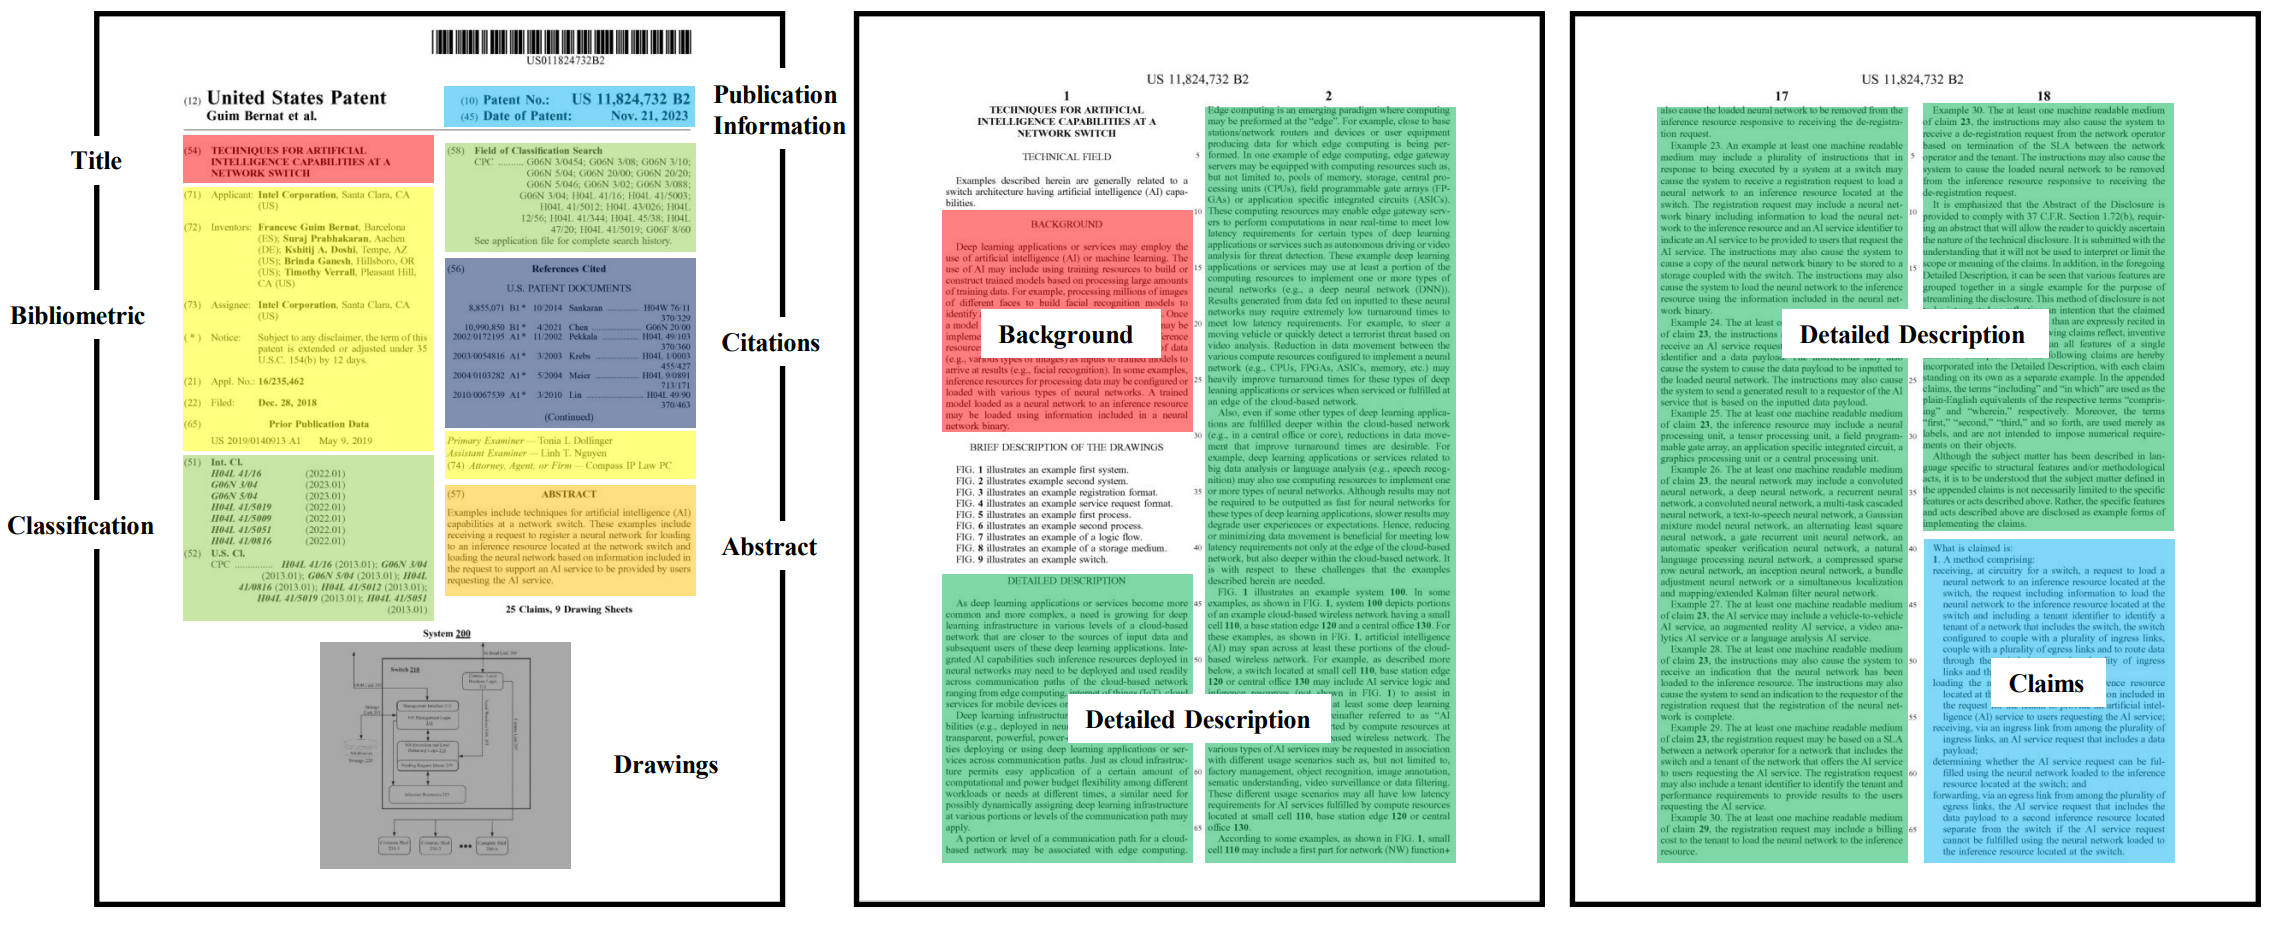
\includegraphics[width=\linewidth]{img/patent.png}
  \caption{Illustration of the structure of a patent from \citet{jiangArtificialIntelligenceExploring2024}. Note that multiple pages from the detailed description are omitted. The description includes all sections except the front matter and claims. In our experiments, we exclude sections containing only metadata, such as statements regarding funding.}
\end{minipage}
\end{figure*}


\FloatBarrier


\begin{table*}
\begin{minipage}{\textwidth}
  \section{Hyperparameters}\label{sec:hyperparameter_appendix}
  \centering
  \begin{tabular}{llcll}
    \toprule
    \multicolumn{2}{c}{Generation} &       & \multicolumn{2}{c}{Training}                                    \\
    \cmidrule{1-2}\cmidrule{4-5}
    Parameter                      & Value &                              & Parameter           & Value      \\
    \midrule
    max sequence length            & 8192  &                              & max sequence length & 8192       \\
    temperature                    & 0.6   &                              & learning rate       & 0.00031622 \\
                                   &       &                              & scheduler           & cosine     \\
                                   &       &                              & warmup ratio        & 0.1        \\
                                   &       &                              & epochs              & 3          \\
                                   &       &                              & batch size          & 32         \\
                                   &       &                              & lora alpha          & 60         \\
                                   &       &                              & lora dropout        & 0.05       \\
                                   &       &                              & lora r              & 128        \\
    \bottomrule
  \end{tabular}
  \caption{Hyperparameters during generation and training. Training parameters are adopted from \citet{tribesHyperparameterOptimizationLarge2024}. We run the experiments on Nvidia H100 80GB GPUs. We use a single H100 for inference and training of the 8B model and 4xH100 for the inference of the larger models using tensor parallel. We estimate the total number of GPU-hours to be 720.}
\end{minipage}
\end{table*}


\FloatBarrier


\renewcommand{\sparqlbasicstyle}{\tiny\tt}
\begin{figure*}
  \section{SPARQL Query}\label{sec:sparql_appendix}
  \begin{minipage}{\textwidth}
  \centering
  \lstinputlisting[language=SPARQL, style=sparqlstyle, caption={SPARQL query template used to retrieve papers for a given patent from SemOpenAlex. Template variables \texttt{<var>} are filled based on the query patent.}]{sections/sparql_query.txt}
\end{minipage}
\end{figure*}
\renewcommand{\sparqlbasicstyle}{\small\tt}


\FloatBarrier


\renewcommand{\sparqlbasicstyle}{\tiny\tt}
\begin{figure*}
  \section{Summary Generation Prompt}\label{sec:summary_prompt_appendix}
  \begin{minipage}{\textwidth}
  \centering
  \lstinputlisting[language=SPARQL, style=sparqlstyle, caption={Prompt used to generate bullet point summaries with Llama-3 70B}]{sections/summary_prompt.txt}
\end{minipage}
\end{figure*}
\renewcommand{\sparqlbasicstyle}{\small\tt}

\FloatBarrier


\renewcommand{\sparqlbasicstyle}{\tiny\tt}
\begin{figure*}
  \section{Patent Generation Prompt}\label{sec:generation_prompt_appendix}
  \begin{minipage}{\textwidth}
  \centering
  \lstinputlisting[language=SPARQL, style=sparqlstyle, caption={System prompt used for outline-guided paper-to-patent generation}]{sections/generation_prompt_system.txt}
\end{minipage}
\end{figure*}

\FloatBarrier


\begin{figure*}
\begin{minipage}{\textwidth}
  \centering
  \lstinputlisting[language=SPARQL, style=sparqlstyle, caption={User prompt used for outline-guided paper-to-patent generation (Part 1)}]{sections/generation_prompt_user_0.txt}
\end{minipage}
\end{figure*}

\begin{figure*}
\begin{minipage}{\textwidth}
  \centering
  \lstinputlisting[language=SPARQL, style=sparqlstyle, caption={User prompt used for outline-guided paper-to-patent generation (Part 2)}]{sections/generation_prompt_user_1.txt}
\end{minipage}
\end{figure*}

\begin{figure*}
\begin{minipage}{\textwidth}
  \centering
  \lstinputlisting[language=SPARQL, style=sparqlstyle, caption={User prompt used for outline-guided paper-to-patent generation (Part 3)}]{sections/generation_prompt_user_2.txt}
\end{minipage}
\end{figure*}

\begin{figure*}
\begin{minipage}{\textwidth}
  \centering
  \lstinputlisting[language=SPARQL, style=sparqlstyle, caption={User prompt used for outline-guided paper-to-patent generation (Part 4)}]{sections/generation_prompt_user_3.txt}
\end{minipage}
\end{figure*}

\renewcommand{\sparqlbasicstyle}{\small\tt}


\FloatBarrier

\begin{figure*}[!ht]
  \section{Dataset Statistics}\label{sec:dataset_stats_appendix}
  \begin{minipage}{\textwidth}
  \centering
  %% Creator: Matplotlib, PGF backend
%%
%% To include the figure in your LaTeX document, write
%%   \input{<filename>.pgf}
%%
%% Make sure the required packages are loaded in your preamble
%%   \usepackage{pgf}
%%
%% Also ensure that all the required font packages are loaded; for instance,
%% the lmodern package is sometimes necessary when using math font.
%%   \usepackage{lmodern}
%%
%% Figures using additional raster images can only be included by \input if
%% they are in the same directory as the main LaTeX file. For loading figures
%% from other directories you can use the `import` package
%%   \usepackage{import}
%%
%% and then include the figures with
%%   \import{<path to file>}{<filename>.pgf}
%%
%% Matplotlib used the following preamble
%%   \def\mathdefault#1{#1}
%%   \everymath=\expandafter{\the\everymath\displaystyle}
%%   
%%   \makeatletter\@ifpackageloaded{underscore}{}{\usepackage[strings]{underscore}}\makeatother
%%
\begingroup%
\makeatletter%
\begin{pgfpicture}%
\pgfpathrectangle{\pgfpointorigin}{\pgfqpoint{5.599828in}{2.000965in}}%
\pgfusepath{use as bounding box, clip}%
\begin{pgfscope}%
\pgfsetbuttcap%
\pgfsetmiterjoin%
\definecolor{currentfill}{rgb}{1.000000,1.000000,1.000000}%
\pgfsetfillcolor{currentfill}%
\pgfsetlinewidth{0.000000pt}%
\definecolor{currentstroke}{rgb}{0.500000,0.500000,0.500000}%
\pgfsetstrokecolor{currentstroke}%
\pgfsetdash{}{0pt}%
\pgfpathmoveto{\pgfqpoint{0.000000in}{0.000000in}}%
\pgfpathlineto{\pgfqpoint{5.599828in}{0.000000in}}%
\pgfpathlineto{\pgfqpoint{5.599828in}{2.000965in}}%
\pgfpathlineto{\pgfqpoint{0.000000in}{2.000965in}}%
\pgfpathlineto{\pgfqpoint{0.000000in}{0.000000in}}%
\pgfpathclose%
\pgfusepath{fill}%
\end{pgfscope}%
\begin{pgfscope}%
\pgfsetbuttcap%
\pgfsetmiterjoin%
\definecolor{currentfill}{rgb}{0.898039,0.898039,0.898039}%
\pgfsetfillcolor{currentfill}%
\pgfsetlinewidth{0.000000pt}%
\definecolor{currentstroke}{rgb}{0.000000,0.000000,0.000000}%
\pgfsetstrokecolor{currentstroke}%
\pgfsetstrokeopacity{0.000000}%
\pgfsetdash{}{0pt}%
\pgfpathmoveto{\pgfqpoint{0.340934in}{0.805783in}}%
\pgfpathlineto{\pgfqpoint{1.349110in}{0.805783in}}%
\pgfpathlineto{\pgfqpoint{1.349110in}{1.730826in}}%
\pgfpathlineto{\pgfqpoint{0.340934in}{1.730826in}}%
\pgfpathlineto{\pgfqpoint{0.340934in}{0.805783in}}%
\pgfpathclose%
\pgfusepath{fill}%
\end{pgfscope}%
\begin{pgfscope}%
\pgfpathrectangle{\pgfqpoint{0.340934in}{0.805783in}}{\pgfqpoint{1.008176in}{0.925043in}}%
\pgfusepath{clip}%
\pgfsetrectcap%
\pgfsetroundjoin%
\pgfsetlinewidth{0.803000pt}%
\definecolor{currentstroke}{rgb}{1.000000,1.000000,1.000000}%
\pgfsetstrokecolor{currentstroke}%
\pgfsetdash{}{0pt}%
\pgfpathmoveto{\pgfqpoint{0.340934in}{0.805783in}}%
\pgfpathlineto{\pgfqpoint{1.349110in}{0.805783in}}%
\pgfusepath{stroke}%
\end{pgfscope}%
\begin{pgfscope}%
\pgfsetbuttcap%
\pgfsetroundjoin%
\definecolor{currentfill}{rgb}{0.333333,0.333333,0.333333}%
\pgfsetfillcolor{currentfill}%
\pgfsetlinewidth{0.803000pt}%
\definecolor{currentstroke}{rgb}{0.333333,0.333333,0.333333}%
\pgfsetstrokecolor{currentstroke}%
\pgfsetdash{}{0pt}%
\pgfsys@defobject{currentmarker}{\pgfqpoint{-0.048611in}{0.000000in}}{\pgfqpoint{-0.000000in}{0.000000in}}{%
\pgfpathmoveto{\pgfqpoint{-0.000000in}{0.000000in}}%
\pgfpathlineto{\pgfqpoint{-0.048611in}{0.000000in}}%
\pgfusepath{stroke,fill}%
}%
\begin{pgfscope}%
\pgfsys@transformshift{0.340934in}{0.805783in}%
\pgfsys@useobject{currentmarker}{}%
\end{pgfscope}%
\end{pgfscope}%
\begin{pgfscope}%
\definecolor{textcolor}{rgb}{0.333333,0.333333,0.333333}%
\pgfsetstrokecolor{textcolor}%
\pgfsetfillcolor{textcolor}%
\pgftext[x=0.100000in, y=0.772025in, left, base]{\color{textcolor}{\rmfamily\fontsize{7.000000}{8.400000}\selectfont\catcode`\^=\active\def^{\ifmmode\sp\else\^{}\fi}\catcode`\%=\active\def%{\%}$\mathdefault{0.0}$}}%
\end{pgfscope}%
\begin{pgfscope}%
\pgfpathrectangle{\pgfqpoint{0.340934in}{0.805783in}}{\pgfqpoint{1.008176in}{0.925043in}}%
\pgfusepath{clip}%
\pgfsetrectcap%
\pgfsetroundjoin%
\pgfsetlinewidth{0.803000pt}%
\definecolor{currentstroke}{rgb}{1.000000,1.000000,1.000000}%
\pgfsetstrokecolor{currentstroke}%
\pgfsetdash{}{0pt}%
\pgfpathmoveto{\pgfqpoint{0.340934in}{1.125151in}}%
\pgfpathlineto{\pgfqpoint{1.349110in}{1.125151in}}%
\pgfusepath{stroke}%
\end{pgfscope}%
\begin{pgfscope}%
\pgfsetbuttcap%
\pgfsetroundjoin%
\definecolor{currentfill}{rgb}{0.333333,0.333333,0.333333}%
\pgfsetfillcolor{currentfill}%
\pgfsetlinewidth{0.803000pt}%
\definecolor{currentstroke}{rgb}{0.333333,0.333333,0.333333}%
\pgfsetstrokecolor{currentstroke}%
\pgfsetdash{}{0pt}%
\pgfsys@defobject{currentmarker}{\pgfqpoint{-0.048611in}{0.000000in}}{\pgfqpoint{-0.000000in}{0.000000in}}{%
\pgfpathmoveto{\pgfqpoint{-0.000000in}{0.000000in}}%
\pgfpathlineto{\pgfqpoint{-0.048611in}{0.000000in}}%
\pgfusepath{stroke,fill}%
}%
\begin{pgfscope}%
\pgfsys@transformshift{0.340934in}{1.125151in}%
\pgfsys@useobject{currentmarker}{}%
\end{pgfscope}%
\end{pgfscope}%
\begin{pgfscope}%
\definecolor{textcolor}{rgb}{0.333333,0.333333,0.333333}%
\pgfsetstrokecolor{textcolor}%
\pgfsetfillcolor{textcolor}%
\pgftext[x=0.100000in, y=1.091394in, left, base]{\color{textcolor}{\rmfamily\fontsize{7.000000}{8.400000}\selectfont\catcode`\^=\active\def^{\ifmmode\sp\else\^{}\fi}\catcode`\%=\active\def%{\%}$\mathdefault{0.2}$}}%
\end{pgfscope}%
\begin{pgfscope}%
\pgfpathrectangle{\pgfqpoint{0.340934in}{0.805783in}}{\pgfqpoint{1.008176in}{0.925043in}}%
\pgfusepath{clip}%
\pgfsetrectcap%
\pgfsetroundjoin%
\pgfsetlinewidth{0.803000pt}%
\definecolor{currentstroke}{rgb}{1.000000,1.000000,1.000000}%
\pgfsetstrokecolor{currentstroke}%
\pgfsetdash{}{0pt}%
\pgfpathmoveto{\pgfqpoint{0.340934in}{1.444519in}}%
\pgfpathlineto{\pgfqpoint{1.349110in}{1.444519in}}%
\pgfusepath{stroke}%
\end{pgfscope}%
\begin{pgfscope}%
\pgfsetbuttcap%
\pgfsetroundjoin%
\definecolor{currentfill}{rgb}{0.333333,0.333333,0.333333}%
\pgfsetfillcolor{currentfill}%
\pgfsetlinewidth{0.803000pt}%
\definecolor{currentstroke}{rgb}{0.333333,0.333333,0.333333}%
\pgfsetstrokecolor{currentstroke}%
\pgfsetdash{}{0pt}%
\pgfsys@defobject{currentmarker}{\pgfqpoint{-0.048611in}{0.000000in}}{\pgfqpoint{-0.000000in}{0.000000in}}{%
\pgfpathmoveto{\pgfqpoint{-0.000000in}{0.000000in}}%
\pgfpathlineto{\pgfqpoint{-0.048611in}{0.000000in}}%
\pgfusepath{stroke,fill}%
}%
\begin{pgfscope}%
\pgfsys@transformshift{0.340934in}{1.444519in}%
\pgfsys@useobject{currentmarker}{}%
\end{pgfscope}%
\end{pgfscope}%
\begin{pgfscope}%
\definecolor{textcolor}{rgb}{0.333333,0.333333,0.333333}%
\pgfsetstrokecolor{textcolor}%
\pgfsetfillcolor{textcolor}%
\pgftext[x=0.100000in, y=1.410762in, left, base]{\color{textcolor}{\rmfamily\fontsize{7.000000}{8.400000}\selectfont\catcode`\^=\active\def^{\ifmmode\sp\else\^{}\fi}\catcode`\%=\active\def%{\%}$\mathdefault{0.4}$}}%
\end{pgfscope}%
\begin{pgfscope}%
\pgfpathrectangle{\pgfqpoint{0.340934in}{0.805783in}}{\pgfqpoint{1.008176in}{0.925043in}}%
\pgfusepath{clip}%
\pgfsetbuttcap%
\pgfsetmiterjoin%
\definecolor{currentfill}{rgb}{0.121569,0.466667,0.705882}%
\pgfsetfillcolor{currentfill}%
\pgfsetlinewidth{0.000000pt}%
\definecolor{currentstroke}{rgb}{0.000000,0.000000,0.000000}%
\pgfsetstrokecolor{currentstroke}%
\pgfsetstrokeopacity{0.000000}%
\pgfsetdash{}{0pt}%
\pgfpathmoveto{\pgfqpoint{0.386760in}{0.805783in}}%
\pgfpathlineto{\pgfqpoint{0.470081in}{0.805783in}}%
\pgfpathlineto{\pgfqpoint{0.470081in}{1.284835in}}%
\pgfpathlineto{\pgfqpoint{0.386760in}{1.284835in}}%
\pgfpathlineto{\pgfqpoint{0.386760in}{0.805783in}}%
\pgfpathclose%
\pgfusepath{fill}%
\end{pgfscope}%
\begin{pgfscope}%
\pgfpathrectangle{\pgfqpoint{0.340934in}{0.805783in}}{\pgfqpoint{1.008176in}{0.925043in}}%
\pgfusepath{clip}%
\pgfsetbuttcap%
\pgfsetmiterjoin%
\definecolor{currentfill}{rgb}{0.682353,0.780392,0.909804}%
\pgfsetfillcolor{currentfill}%
\pgfsetlinewidth{0.000000pt}%
\definecolor{currentstroke}{rgb}{0.000000,0.000000,0.000000}%
\pgfsetstrokecolor{currentstroke}%
\pgfsetstrokeopacity{0.000000}%
\pgfsetdash{}{0pt}%
\pgfpathmoveto{\pgfqpoint{0.490911in}{0.805783in}}%
\pgfpathlineto{\pgfqpoint{0.574231in}{0.805783in}}%
\pgfpathlineto{\pgfqpoint{0.574231in}{1.204993in}}%
\pgfpathlineto{\pgfqpoint{0.490911in}{1.204993in}}%
\pgfpathlineto{\pgfqpoint{0.490911in}{0.805783in}}%
\pgfpathclose%
\pgfusepath{fill}%
\end{pgfscope}%
\begin{pgfscope}%
\pgfpathrectangle{\pgfqpoint{0.340934in}{0.805783in}}{\pgfqpoint{1.008176in}{0.925043in}}%
\pgfusepath{clip}%
\pgfsetbuttcap%
\pgfsetmiterjoin%
\definecolor{currentfill}{rgb}{1.000000,0.498039,0.054902}%
\pgfsetfillcolor{currentfill}%
\pgfsetlinewidth{0.000000pt}%
\definecolor{currentstroke}{rgb}{0.000000,0.000000,0.000000}%
\pgfsetstrokecolor{currentstroke}%
\pgfsetstrokeopacity{0.000000}%
\pgfsetdash{}{0pt}%
\pgfpathmoveto{\pgfqpoint{0.595061in}{0.805783in}}%
\pgfpathlineto{\pgfqpoint{0.678381in}{0.805783in}}%
\pgfpathlineto{\pgfqpoint{0.678381in}{1.022953in}}%
\pgfpathlineto{\pgfqpoint{0.595061in}{1.022953in}}%
\pgfpathlineto{\pgfqpoint{0.595061in}{0.805783in}}%
\pgfpathclose%
\pgfusepath{fill}%
\end{pgfscope}%
\begin{pgfscope}%
\pgfpathrectangle{\pgfqpoint{0.340934in}{0.805783in}}{\pgfqpoint{1.008176in}{0.925043in}}%
\pgfusepath{clip}%
\pgfsetbuttcap%
\pgfsetmiterjoin%
\definecolor{currentfill}{rgb}{1.000000,0.733333,0.470588}%
\pgfsetfillcolor{currentfill}%
\pgfsetlinewidth{0.000000pt}%
\definecolor{currentstroke}{rgb}{0.000000,0.000000,0.000000}%
\pgfsetstrokecolor{currentstroke}%
\pgfsetstrokeopacity{0.000000}%
\pgfsetdash{}{0pt}%
\pgfpathmoveto{\pgfqpoint{0.699211in}{0.805783in}}%
\pgfpathlineto{\pgfqpoint{0.782532in}{0.805783in}}%
\pgfpathlineto{\pgfqpoint{0.782532in}{1.018163in}}%
\pgfpathlineto{\pgfqpoint{0.699211in}{1.018163in}}%
\pgfpathlineto{\pgfqpoint{0.699211in}{0.805783in}}%
\pgfpathclose%
\pgfusepath{fill}%
\end{pgfscope}%
\begin{pgfscope}%
\pgfpathrectangle{\pgfqpoint{0.340934in}{0.805783in}}{\pgfqpoint{1.008176in}{0.925043in}}%
\pgfusepath{clip}%
\pgfsetbuttcap%
\pgfsetmiterjoin%
\definecolor{currentfill}{rgb}{0.172549,0.627451,0.172549}%
\pgfsetfillcolor{currentfill}%
\pgfsetlinewidth{0.000000pt}%
\definecolor{currentstroke}{rgb}{0.000000,0.000000,0.000000}%
\pgfsetstrokecolor{currentstroke}%
\pgfsetstrokeopacity{0.000000}%
\pgfsetdash{}{0pt}%
\pgfpathmoveto{\pgfqpoint{0.803362in}{0.805783in}}%
\pgfpathlineto{\pgfqpoint{0.886682in}{0.805783in}}%
\pgfpathlineto{\pgfqpoint{0.886682in}{1.013372in}}%
\pgfpathlineto{\pgfqpoint{0.803362in}{1.013372in}}%
\pgfpathlineto{\pgfqpoint{0.803362in}{0.805783in}}%
\pgfpathclose%
\pgfusepath{fill}%
\end{pgfscope}%
\begin{pgfscope}%
\pgfpathrectangle{\pgfqpoint{0.340934in}{0.805783in}}{\pgfqpoint{1.008176in}{0.925043in}}%
\pgfusepath{clip}%
\pgfsetbuttcap%
\pgfsetmiterjoin%
\definecolor{currentfill}{rgb}{0.596078,0.874510,0.541176}%
\pgfsetfillcolor{currentfill}%
\pgfsetlinewidth{0.000000pt}%
\definecolor{currentstroke}{rgb}{0.000000,0.000000,0.000000}%
\pgfsetstrokecolor{currentstroke}%
\pgfsetstrokeopacity{0.000000}%
\pgfsetdash{}{0pt}%
\pgfpathmoveto{\pgfqpoint{0.907512in}{0.805783in}}%
\pgfpathlineto{\pgfqpoint{0.990833in}{0.805783in}}%
\pgfpathlineto{\pgfqpoint{0.990833in}{0.848898in}}%
\pgfpathlineto{\pgfqpoint{0.907512in}{0.848898in}}%
\pgfpathlineto{\pgfqpoint{0.907512in}{0.805783in}}%
\pgfpathclose%
\pgfusepath{fill}%
\end{pgfscope}%
\begin{pgfscope}%
\pgfpathrectangle{\pgfqpoint{0.340934in}{0.805783in}}{\pgfqpoint{1.008176in}{0.925043in}}%
\pgfusepath{clip}%
\pgfsetbuttcap%
\pgfsetmiterjoin%
\definecolor{currentfill}{rgb}{0.839216,0.152941,0.156863}%
\pgfsetfillcolor{currentfill}%
\pgfsetlinewidth{0.000000pt}%
\definecolor{currentstroke}{rgb}{0.000000,0.000000,0.000000}%
\pgfsetstrokecolor{currentstroke}%
\pgfsetstrokeopacity{0.000000}%
\pgfsetdash{}{0pt}%
\pgfpathmoveto{\pgfqpoint{1.011663in}{0.805783in}}%
\pgfpathlineto{\pgfqpoint{1.094983in}{0.805783in}}%
\pgfpathlineto{\pgfqpoint{1.094983in}{0.824945in}}%
\pgfpathlineto{\pgfqpoint{1.011663in}{0.824945in}}%
\pgfpathlineto{\pgfqpoint{1.011663in}{0.805783in}}%
\pgfpathclose%
\pgfusepath{fill}%
\end{pgfscope}%
\begin{pgfscope}%
\pgfpathrectangle{\pgfqpoint{0.340934in}{0.805783in}}{\pgfqpoint{1.008176in}{0.925043in}}%
\pgfusepath{clip}%
\pgfsetbuttcap%
\pgfsetmiterjoin%
\definecolor{currentfill}{rgb}{1.000000,0.596078,0.588235}%
\pgfsetfillcolor{currentfill}%
\pgfsetlinewidth{0.000000pt}%
\definecolor{currentstroke}{rgb}{0.000000,0.000000,0.000000}%
\pgfsetstrokecolor{currentstroke}%
\pgfsetstrokeopacity{0.000000}%
\pgfsetdash{}{0pt}%
\pgfpathmoveto{\pgfqpoint{1.115813in}{0.805783in}}%
\pgfpathlineto{\pgfqpoint{1.199133in}{0.805783in}}%
\pgfpathlineto{\pgfqpoint{1.199133in}{0.813767in}}%
\pgfpathlineto{\pgfqpoint{1.115813in}{0.813767in}}%
\pgfpathlineto{\pgfqpoint{1.115813in}{0.805783in}}%
\pgfpathclose%
\pgfusepath{fill}%
\end{pgfscope}%
\begin{pgfscope}%
\pgfpathrectangle{\pgfqpoint{0.340934in}{0.805783in}}{\pgfqpoint{1.008176in}{0.925043in}}%
\pgfusepath{clip}%
\pgfsetbuttcap%
\pgfsetmiterjoin%
\definecolor{currentfill}{rgb}{0.580392,0.403922,0.741176}%
\pgfsetfillcolor{currentfill}%
\pgfsetlinewidth{0.000000pt}%
\definecolor{currentstroke}{rgb}{0.000000,0.000000,0.000000}%
\pgfsetstrokecolor{currentstroke}%
\pgfsetstrokeopacity{0.000000}%
\pgfsetdash{}{0pt}%
\pgfpathmoveto{\pgfqpoint{1.219963in}{0.805783in}}%
\pgfpathlineto{\pgfqpoint{1.303284in}{0.805783in}}%
\pgfpathlineto{\pgfqpoint{1.303284in}{0.816961in}}%
\pgfpathlineto{\pgfqpoint{1.219963in}{0.816961in}}%
\pgfpathlineto{\pgfqpoint{1.219963in}{0.805783in}}%
\pgfpathclose%
\pgfusepath{fill}%
\end{pgfscope}%
\begin{pgfscope}%
\pgfsetrectcap%
\pgfsetmiterjoin%
\pgfsetlinewidth{1.003750pt}%
\definecolor{currentstroke}{rgb}{1.000000,1.000000,1.000000}%
\pgfsetstrokecolor{currentstroke}%
\pgfsetdash{}{0pt}%
\pgfpathmoveto{\pgfqpoint{0.340934in}{0.805783in}}%
\pgfpathlineto{\pgfqpoint{0.340934in}{1.730826in}}%
\pgfusepath{stroke}%
\end{pgfscope}%
\begin{pgfscope}%
\pgfsetrectcap%
\pgfsetmiterjoin%
\pgfsetlinewidth{1.003750pt}%
\definecolor{currentstroke}{rgb}{1.000000,1.000000,1.000000}%
\pgfsetstrokecolor{currentstroke}%
\pgfsetdash{}{0pt}%
\pgfpathmoveto{\pgfqpoint{1.349110in}{0.805783in}}%
\pgfpathlineto{\pgfqpoint{1.349110in}{1.730826in}}%
\pgfusepath{stroke}%
\end{pgfscope}%
\begin{pgfscope}%
\pgfsetrectcap%
\pgfsetmiterjoin%
\pgfsetlinewidth{1.003750pt}%
\definecolor{currentstroke}{rgb}{1.000000,1.000000,1.000000}%
\pgfsetstrokecolor{currentstroke}%
\pgfsetdash{}{0pt}%
\pgfpathmoveto{\pgfqpoint{0.340934in}{0.805783in}}%
\pgfpathlineto{\pgfqpoint{1.349110in}{0.805783in}}%
\pgfusepath{stroke}%
\end{pgfscope}%
\begin{pgfscope}%
\pgfsetrectcap%
\pgfsetmiterjoin%
\pgfsetlinewidth{1.003750pt}%
\definecolor{currentstroke}{rgb}{1.000000,1.000000,1.000000}%
\pgfsetstrokecolor{currentstroke}%
\pgfsetdash{}{0pt}%
\pgfpathmoveto{\pgfqpoint{0.340934in}{1.730826in}}%
\pgfpathlineto{\pgfqpoint{1.349110in}{1.730826in}}%
\pgfusepath{stroke}%
\end{pgfscope}%
\begin{pgfscope}%
\definecolor{textcolor}{rgb}{0.000000,0.000000,0.000000}%
\pgfsetstrokecolor{textcolor}%
\pgfsetfillcolor{textcolor}%
\pgftext[x=0.845022in,y=1.814160in,,base]{\color{textcolor}{\rmfamily\fontsize{9.000000}{10.800000}\selectfont\catcode`\^=\active\def^{\ifmmode\sp\else\^{}\fi}\catcode`\%=\active\def%{\%}train}}%
\end{pgfscope}%
\begin{pgfscope}%
\pgfsetbuttcap%
\pgfsetmiterjoin%
\definecolor{currentfill}{rgb}{0.898039,0.898039,0.898039}%
\pgfsetfillcolor{currentfill}%
\pgfsetlinewidth{0.000000pt}%
\definecolor{currentstroke}{rgb}{0.000000,0.000000,0.000000}%
\pgfsetstrokecolor{currentstroke}%
\pgfsetstrokeopacity{0.000000}%
\pgfsetdash{}{0pt}%
\pgfpathmoveto{\pgfqpoint{1.724507in}{0.805783in}}%
\pgfpathlineto{\pgfqpoint{2.732683in}{0.805783in}}%
\pgfpathlineto{\pgfqpoint{2.732683in}{1.730826in}}%
\pgfpathlineto{\pgfqpoint{1.724507in}{1.730826in}}%
\pgfpathlineto{\pgfqpoint{1.724507in}{0.805783in}}%
\pgfpathclose%
\pgfusepath{fill}%
\end{pgfscope}%
\begin{pgfscope}%
\pgfpathrectangle{\pgfqpoint{1.724507in}{0.805783in}}{\pgfqpoint{1.008176in}{0.925043in}}%
\pgfusepath{clip}%
\pgfsetrectcap%
\pgfsetroundjoin%
\pgfsetlinewidth{0.803000pt}%
\definecolor{currentstroke}{rgb}{1.000000,1.000000,1.000000}%
\pgfsetstrokecolor{currentstroke}%
\pgfsetdash{}{0pt}%
\pgfpathmoveto{\pgfqpoint{1.724507in}{0.805783in}}%
\pgfpathlineto{\pgfqpoint{2.732683in}{0.805783in}}%
\pgfusepath{stroke}%
\end{pgfscope}%
\begin{pgfscope}%
\pgfsetbuttcap%
\pgfsetroundjoin%
\definecolor{currentfill}{rgb}{0.333333,0.333333,0.333333}%
\pgfsetfillcolor{currentfill}%
\pgfsetlinewidth{0.803000pt}%
\definecolor{currentstroke}{rgb}{0.333333,0.333333,0.333333}%
\pgfsetstrokecolor{currentstroke}%
\pgfsetdash{}{0pt}%
\pgfsys@defobject{currentmarker}{\pgfqpoint{-0.048611in}{0.000000in}}{\pgfqpoint{-0.000000in}{0.000000in}}{%
\pgfpathmoveto{\pgfqpoint{-0.000000in}{0.000000in}}%
\pgfpathlineto{\pgfqpoint{-0.048611in}{0.000000in}}%
\pgfusepath{stroke,fill}%
}%
\begin{pgfscope}%
\pgfsys@transformshift{1.724507in}{0.805783in}%
\pgfsys@useobject{currentmarker}{}%
\end{pgfscope}%
\end{pgfscope}%
\begin{pgfscope}%
\definecolor{textcolor}{rgb}{0.333333,0.333333,0.333333}%
\pgfsetstrokecolor{textcolor}%
\pgfsetfillcolor{textcolor}%
\pgftext[x=1.483573in, y=0.772025in, left, base]{\color{textcolor}{\rmfamily\fontsize{7.000000}{8.400000}\selectfont\catcode`\^=\active\def^{\ifmmode\sp\else\^{}\fi}\catcode`\%=\active\def%{\%}$\mathdefault{0.0}$}}%
\end{pgfscope}%
\begin{pgfscope}%
\pgfpathrectangle{\pgfqpoint{1.724507in}{0.805783in}}{\pgfqpoint{1.008176in}{0.925043in}}%
\pgfusepath{clip}%
\pgfsetrectcap%
\pgfsetroundjoin%
\pgfsetlinewidth{0.803000pt}%
\definecolor{currentstroke}{rgb}{1.000000,1.000000,1.000000}%
\pgfsetstrokecolor{currentstroke}%
\pgfsetdash{}{0pt}%
\pgfpathmoveto{\pgfqpoint{1.724507in}{1.125151in}}%
\pgfpathlineto{\pgfqpoint{2.732683in}{1.125151in}}%
\pgfusepath{stroke}%
\end{pgfscope}%
\begin{pgfscope}%
\pgfsetbuttcap%
\pgfsetroundjoin%
\definecolor{currentfill}{rgb}{0.333333,0.333333,0.333333}%
\pgfsetfillcolor{currentfill}%
\pgfsetlinewidth{0.803000pt}%
\definecolor{currentstroke}{rgb}{0.333333,0.333333,0.333333}%
\pgfsetstrokecolor{currentstroke}%
\pgfsetdash{}{0pt}%
\pgfsys@defobject{currentmarker}{\pgfqpoint{-0.048611in}{0.000000in}}{\pgfqpoint{-0.000000in}{0.000000in}}{%
\pgfpathmoveto{\pgfqpoint{-0.000000in}{0.000000in}}%
\pgfpathlineto{\pgfqpoint{-0.048611in}{0.000000in}}%
\pgfusepath{stroke,fill}%
}%
\begin{pgfscope}%
\pgfsys@transformshift{1.724507in}{1.125151in}%
\pgfsys@useobject{currentmarker}{}%
\end{pgfscope}%
\end{pgfscope}%
\begin{pgfscope}%
\definecolor{textcolor}{rgb}{0.333333,0.333333,0.333333}%
\pgfsetstrokecolor{textcolor}%
\pgfsetfillcolor{textcolor}%
\pgftext[x=1.483573in, y=1.091394in, left, base]{\color{textcolor}{\rmfamily\fontsize{7.000000}{8.400000}\selectfont\catcode`\^=\active\def^{\ifmmode\sp\else\^{}\fi}\catcode`\%=\active\def%{\%}$\mathdefault{0.2}$}}%
\end{pgfscope}%
\begin{pgfscope}%
\pgfpathrectangle{\pgfqpoint{1.724507in}{0.805783in}}{\pgfqpoint{1.008176in}{0.925043in}}%
\pgfusepath{clip}%
\pgfsetrectcap%
\pgfsetroundjoin%
\pgfsetlinewidth{0.803000pt}%
\definecolor{currentstroke}{rgb}{1.000000,1.000000,1.000000}%
\pgfsetstrokecolor{currentstroke}%
\pgfsetdash{}{0pt}%
\pgfpathmoveto{\pgfqpoint{1.724507in}{1.444519in}}%
\pgfpathlineto{\pgfqpoint{2.732683in}{1.444519in}}%
\pgfusepath{stroke}%
\end{pgfscope}%
\begin{pgfscope}%
\pgfsetbuttcap%
\pgfsetroundjoin%
\definecolor{currentfill}{rgb}{0.333333,0.333333,0.333333}%
\pgfsetfillcolor{currentfill}%
\pgfsetlinewidth{0.803000pt}%
\definecolor{currentstroke}{rgb}{0.333333,0.333333,0.333333}%
\pgfsetstrokecolor{currentstroke}%
\pgfsetdash{}{0pt}%
\pgfsys@defobject{currentmarker}{\pgfqpoint{-0.048611in}{0.000000in}}{\pgfqpoint{-0.000000in}{0.000000in}}{%
\pgfpathmoveto{\pgfqpoint{-0.000000in}{0.000000in}}%
\pgfpathlineto{\pgfqpoint{-0.048611in}{0.000000in}}%
\pgfusepath{stroke,fill}%
}%
\begin{pgfscope}%
\pgfsys@transformshift{1.724507in}{1.444519in}%
\pgfsys@useobject{currentmarker}{}%
\end{pgfscope}%
\end{pgfscope}%
\begin{pgfscope}%
\definecolor{textcolor}{rgb}{0.333333,0.333333,0.333333}%
\pgfsetstrokecolor{textcolor}%
\pgfsetfillcolor{textcolor}%
\pgftext[x=1.483573in, y=1.410762in, left, base]{\color{textcolor}{\rmfamily\fontsize{7.000000}{8.400000}\selectfont\catcode`\^=\active\def^{\ifmmode\sp\else\^{}\fi}\catcode`\%=\active\def%{\%}$\mathdefault{0.4}$}}%
\end{pgfscope}%
\begin{pgfscope}%
\pgfpathrectangle{\pgfqpoint{1.724507in}{0.805783in}}{\pgfqpoint{1.008176in}{0.925043in}}%
\pgfusepath{clip}%
\pgfsetbuttcap%
\pgfsetmiterjoin%
\definecolor{currentfill}{rgb}{0.121569,0.466667,0.705882}%
\pgfsetfillcolor{currentfill}%
\pgfsetlinewidth{0.000000pt}%
\definecolor{currentstroke}{rgb}{0.000000,0.000000,0.000000}%
\pgfsetstrokecolor{currentstroke}%
\pgfsetstrokeopacity{0.000000}%
\pgfsetdash{}{0pt}%
\pgfpathmoveto{\pgfqpoint{1.770333in}{0.805783in}}%
\pgfpathlineto{\pgfqpoint{1.853654in}{0.805783in}}%
\pgfpathlineto{\pgfqpoint{1.853654in}{1.221490in}}%
\pgfpathlineto{\pgfqpoint{1.770333in}{1.221490in}}%
\pgfpathlineto{\pgfqpoint{1.770333in}{0.805783in}}%
\pgfpathclose%
\pgfusepath{fill}%
\end{pgfscope}%
\begin{pgfscope}%
\pgfpathrectangle{\pgfqpoint{1.724507in}{0.805783in}}{\pgfqpoint{1.008176in}{0.925043in}}%
\pgfusepath{clip}%
\pgfsetbuttcap%
\pgfsetmiterjoin%
\definecolor{currentfill}{rgb}{0.682353,0.780392,0.909804}%
\pgfsetfillcolor{currentfill}%
\pgfsetlinewidth{0.000000pt}%
\definecolor{currentstroke}{rgb}{0.000000,0.000000,0.000000}%
\pgfsetstrokecolor{currentstroke}%
\pgfsetstrokeopacity{0.000000}%
\pgfsetdash{}{0pt}%
\pgfpathmoveto{\pgfqpoint{1.874484in}{0.805783in}}%
\pgfpathlineto{\pgfqpoint{1.957804in}{0.805783in}}%
\pgfpathlineto{\pgfqpoint{1.957804in}{1.175300in}}%
\pgfpathlineto{\pgfqpoint{1.874484in}{1.175300in}}%
\pgfpathlineto{\pgfqpoint{1.874484in}{0.805783in}}%
\pgfpathclose%
\pgfusepath{fill}%
\end{pgfscope}%
\begin{pgfscope}%
\pgfpathrectangle{\pgfqpoint{1.724507in}{0.805783in}}{\pgfqpoint{1.008176in}{0.925043in}}%
\pgfusepath{clip}%
\pgfsetbuttcap%
\pgfsetmiterjoin%
\definecolor{currentfill}{rgb}{1.000000,0.498039,0.054902}%
\pgfsetfillcolor{currentfill}%
\pgfsetlinewidth{0.000000pt}%
\definecolor{currentstroke}{rgb}{0.000000,0.000000,0.000000}%
\pgfsetstrokecolor{currentstroke}%
\pgfsetstrokeopacity{0.000000}%
\pgfsetdash{}{0pt}%
\pgfpathmoveto{\pgfqpoint{1.978634in}{0.805783in}}%
\pgfpathlineto{\pgfqpoint{2.061954in}{0.805783in}}%
\pgfpathlineto{\pgfqpoint{2.061954in}{1.069724in}}%
\pgfpathlineto{\pgfqpoint{1.978634in}{1.069724in}}%
\pgfpathlineto{\pgfqpoint{1.978634in}{0.805783in}}%
\pgfpathclose%
\pgfusepath{fill}%
\end{pgfscope}%
\begin{pgfscope}%
\pgfpathrectangle{\pgfqpoint{1.724507in}{0.805783in}}{\pgfqpoint{1.008176in}{0.925043in}}%
\pgfusepath{clip}%
\pgfsetbuttcap%
\pgfsetmiterjoin%
\definecolor{currentfill}{rgb}{1.000000,0.733333,0.470588}%
\pgfsetfillcolor{currentfill}%
\pgfsetlinewidth{0.000000pt}%
\definecolor{currentstroke}{rgb}{0.000000,0.000000,0.000000}%
\pgfsetstrokecolor{currentstroke}%
\pgfsetstrokeopacity{0.000000}%
\pgfsetdash{}{0pt}%
\pgfpathmoveto{\pgfqpoint{2.082784in}{0.805783in}}%
\pgfpathlineto{\pgfqpoint{2.166105in}{0.805783in}}%
\pgfpathlineto{\pgfqpoint{2.166105in}{1.023534in}}%
\pgfpathlineto{\pgfqpoint{2.082784in}{1.023534in}}%
\pgfpathlineto{\pgfqpoint{2.082784in}{0.805783in}}%
\pgfpathclose%
\pgfusepath{fill}%
\end{pgfscope}%
\begin{pgfscope}%
\pgfpathrectangle{\pgfqpoint{1.724507in}{0.805783in}}{\pgfqpoint{1.008176in}{0.925043in}}%
\pgfusepath{clip}%
\pgfsetbuttcap%
\pgfsetmiterjoin%
\definecolor{currentfill}{rgb}{0.172549,0.627451,0.172549}%
\pgfsetfillcolor{currentfill}%
\pgfsetlinewidth{0.000000pt}%
\definecolor{currentstroke}{rgb}{0.000000,0.000000,0.000000}%
\pgfsetstrokecolor{currentstroke}%
\pgfsetstrokeopacity{0.000000}%
\pgfsetdash{}{0pt}%
\pgfpathmoveto{\pgfqpoint{2.186935in}{0.805783in}}%
\pgfpathlineto{\pgfqpoint{2.270255in}{0.805783in}}%
\pgfpathlineto{\pgfqpoint{2.270255in}{1.069724in}}%
\pgfpathlineto{\pgfqpoint{2.186935in}{1.069724in}}%
\pgfpathlineto{\pgfqpoint{2.186935in}{0.805783in}}%
\pgfpathclose%
\pgfusepath{fill}%
\end{pgfscope}%
\begin{pgfscope}%
\pgfpathrectangle{\pgfqpoint{1.724507in}{0.805783in}}{\pgfqpoint{1.008176in}{0.925043in}}%
\pgfusepath{clip}%
\pgfsetbuttcap%
\pgfsetmiterjoin%
\definecolor{currentfill}{rgb}{0.596078,0.874510,0.541176}%
\pgfsetfillcolor{currentfill}%
\pgfsetlinewidth{0.000000pt}%
\definecolor{currentstroke}{rgb}{0.000000,0.000000,0.000000}%
\pgfsetstrokecolor{currentstroke}%
\pgfsetstrokeopacity{0.000000}%
\pgfsetdash{}{0pt}%
\pgfpathmoveto{\pgfqpoint{2.291085in}{0.805783in}}%
\pgfpathlineto{\pgfqpoint{2.374405in}{0.805783in}}%
\pgfpathlineto{\pgfqpoint{2.374405in}{0.825579in}}%
\pgfpathlineto{\pgfqpoint{2.291085in}{0.825579in}}%
\pgfpathlineto{\pgfqpoint{2.291085in}{0.805783in}}%
\pgfpathclose%
\pgfusepath{fill}%
\end{pgfscope}%
\begin{pgfscope}%
\pgfpathrectangle{\pgfqpoint{1.724507in}{0.805783in}}{\pgfqpoint{1.008176in}{0.925043in}}%
\pgfusepath{clip}%
\pgfsetbuttcap%
\pgfsetmiterjoin%
\definecolor{currentfill}{rgb}{0.839216,0.152941,0.156863}%
\pgfsetfillcolor{currentfill}%
\pgfsetlinewidth{0.000000pt}%
\definecolor{currentstroke}{rgb}{0.000000,0.000000,0.000000}%
\pgfsetstrokecolor{currentstroke}%
\pgfsetstrokeopacity{0.000000}%
\pgfsetdash{}{0pt}%
\pgfpathmoveto{\pgfqpoint{2.395235in}{0.805783in}}%
\pgfpathlineto{\pgfqpoint{2.478556in}{0.805783in}}%
\pgfpathlineto{\pgfqpoint{2.478556in}{0.818980in}}%
\pgfpathlineto{\pgfqpoint{2.395235in}{0.818980in}}%
\pgfpathlineto{\pgfqpoint{2.395235in}{0.805783in}}%
\pgfpathclose%
\pgfusepath{fill}%
\end{pgfscope}%
\begin{pgfscope}%
\pgfpathrectangle{\pgfqpoint{1.724507in}{0.805783in}}{\pgfqpoint{1.008176in}{0.925043in}}%
\pgfusepath{clip}%
\pgfsetbuttcap%
\pgfsetmiterjoin%
\definecolor{currentfill}{rgb}{1.000000,0.596078,0.588235}%
\pgfsetfillcolor{currentfill}%
\pgfsetlinewidth{0.000000pt}%
\definecolor{currentstroke}{rgb}{0.000000,0.000000,0.000000}%
\pgfsetstrokecolor{currentstroke}%
\pgfsetstrokeopacity{0.000000}%
\pgfsetdash{}{0pt}%
\pgfpathmoveto{\pgfqpoint{2.499386in}{0.805783in}}%
\pgfpathlineto{\pgfqpoint{2.582706in}{0.805783in}}%
\pgfpathlineto{\pgfqpoint{2.582706in}{0.818980in}}%
\pgfpathlineto{\pgfqpoint{2.499386in}{0.818980in}}%
\pgfpathlineto{\pgfqpoint{2.499386in}{0.805783in}}%
\pgfpathclose%
\pgfusepath{fill}%
\end{pgfscope}%
\begin{pgfscope}%
\pgfpathrectangle{\pgfqpoint{1.724507in}{0.805783in}}{\pgfqpoint{1.008176in}{0.925043in}}%
\pgfusepath{clip}%
\pgfsetbuttcap%
\pgfsetmiterjoin%
\definecolor{currentfill}{rgb}{0.580392,0.403922,0.741176}%
\pgfsetfillcolor{currentfill}%
\pgfsetlinewidth{0.000000pt}%
\definecolor{currentstroke}{rgb}{0.000000,0.000000,0.000000}%
\pgfsetstrokecolor{currentstroke}%
\pgfsetstrokeopacity{0.000000}%
\pgfsetdash{}{0pt}%
\pgfpathmoveto{\pgfqpoint{2.603536in}{0.805783in}}%
\pgfpathlineto{\pgfqpoint{2.686857in}{0.805783in}}%
\pgfpathlineto{\pgfqpoint{2.686857in}{0.825579in}}%
\pgfpathlineto{\pgfqpoint{2.603536in}{0.825579in}}%
\pgfpathlineto{\pgfqpoint{2.603536in}{0.805783in}}%
\pgfpathclose%
\pgfusepath{fill}%
\end{pgfscope}%
\begin{pgfscope}%
\pgfsetrectcap%
\pgfsetmiterjoin%
\pgfsetlinewidth{1.003750pt}%
\definecolor{currentstroke}{rgb}{1.000000,1.000000,1.000000}%
\pgfsetstrokecolor{currentstroke}%
\pgfsetdash{}{0pt}%
\pgfpathmoveto{\pgfqpoint{1.724507in}{0.805783in}}%
\pgfpathlineto{\pgfqpoint{1.724507in}{1.730826in}}%
\pgfusepath{stroke}%
\end{pgfscope}%
\begin{pgfscope}%
\pgfsetrectcap%
\pgfsetmiterjoin%
\pgfsetlinewidth{1.003750pt}%
\definecolor{currentstroke}{rgb}{1.000000,1.000000,1.000000}%
\pgfsetstrokecolor{currentstroke}%
\pgfsetdash{}{0pt}%
\pgfpathmoveto{\pgfqpoint{2.732683in}{0.805783in}}%
\pgfpathlineto{\pgfqpoint{2.732683in}{1.730826in}}%
\pgfusepath{stroke}%
\end{pgfscope}%
\begin{pgfscope}%
\pgfsetrectcap%
\pgfsetmiterjoin%
\pgfsetlinewidth{1.003750pt}%
\definecolor{currentstroke}{rgb}{1.000000,1.000000,1.000000}%
\pgfsetstrokecolor{currentstroke}%
\pgfsetdash{}{0pt}%
\pgfpathmoveto{\pgfqpoint{1.724507in}{0.805783in}}%
\pgfpathlineto{\pgfqpoint{2.732683in}{0.805783in}}%
\pgfusepath{stroke}%
\end{pgfscope}%
\begin{pgfscope}%
\pgfsetrectcap%
\pgfsetmiterjoin%
\pgfsetlinewidth{1.003750pt}%
\definecolor{currentstroke}{rgb}{1.000000,1.000000,1.000000}%
\pgfsetstrokecolor{currentstroke}%
\pgfsetdash{}{0pt}%
\pgfpathmoveto{\pgfqpoint{1.724507in}{1.730826in}}%
\pgfpathlineto{\pgfqpoint{2.732683in}{1.730826in}}%
\pgfusepath{stroke}%
\end{pgfscope}%
\begin{pgfscope}%
\definecolor{textcolor}{rgb}{0.000000,0.000000,0.000000}%
\pgfsetstrokecolor{textcolor}%
\pgfsetfillcolor{textcolor}%
\pgftext[x=2.228595in,y=1.814160in,,base]{\color{textcolor}{\rmfamily\fontsize{9.000000}{10.800000}\selectfont\catcode`\^=\active\def^{\ifmmode\sp\else\^{}\fi}\catcode`\%=\active\def%{\%}val}}%
\end{pgfscope}%
\begin{pgfscope}%
\pgfsetbuttcap%
\pgfsetmiterjoin%
\definecolor{currentfill}{rgb}{0.898039,0.898039,0.898039}%
\pgfsetfillcolor{currentfill}%
\pgfsetlinewidth{0.000000pt}%
\definecolor{currentstroke}{rgb}{0.000000,0.000000,0.000000}%
\pgfsetstrokecolor{currentstroke}%
\pgfsetstrokeopacity{0.000000}%
\pgfsetdash{}{0pt}%
\pgfpathmoveto{\pgfqpoint{3.108080in}{0.805783in}}%
\pgfpathlineto{\pgfqpoint{4.116256in}{0.805783in}}%
\pgfpathlineto{\pgfqpoint{4.116256in}{1.730826in}}%
\pgfpathlineto{\pgfqpoint{3.108080in}{1.730826in}}%
\pgfpathlineto{\pgfqpoint{3.108080in}{0.805783in}}%
\pgfpathclose%
\pgfusepath{fill}%
\end{pgfscope}%
\begin{pgfscope}%
\pgfpathrectangle{\pgfqpoint{3.108080in}{0.805783in}}{\pgfqpoint{1.008176in}{0.925043in}}%
\pgfusepath{clip}%
\pgfsetrectcap%
\pgfsetroundjoin%
\pgfsetlinewidth{0.803000pt}%
\definecolor{currentstroke}{rgb}{1.000000,1.000000,1.000000}%
\pgfsetstrokecolor{currentstroke}%
\pgfsetdash{}{0pt}%
\pgfpathmoveto{\pgfqpoint{3.108080in}{0.805783in}}%
\pgfpathlineto{\pgfqpoint{4.116256in}{0.805783in}}%
\pgfusepath{stroke}%
\end{pgfscope}%
\begin{pgfscope}%
\pgfsetbuttcap%
\pgfsetroundjoin%
\definecolor{currentfill}{rgb}{0.333333,0.333333,0.333333}%
\pgfsetfillcolor{currentfill}%
\pgfsetlinewidth{0.803000pt}%
\definecolor{currentstroke}{rgb}{0.333333,0.333333,0.333333}%
\pgfsetstrokecolor{currentstroke}%
\pgfsetdash{}{0pt}%
\pgfsys@defobject{currentmarker}{\pgfqpoint{-0.048611in}{0.000000in}}{\pgfqpoint{-0.000000in}{0.000000in}}{%
\pgfpathmoveto{\pgfqpoint{-0.000000in}{0.000000in}}%
\pgfpathlineto{\pgfqpoint{-0.048611in}{0.000000in}}%
\pgfusepath{stroke,fill}%
}%
\begin{pgfscope}%
\pgfsys@transformshift{3.108080in}{0.805783in}%
\pgfsys@useobject{currentmarker}{}%
\end{pgfscope}%
\end{pgfscope}%
\begin{pgfscope}%
\definecolor{textcolor}{rgb}{0.333333,0.333333,0.333333}%
\pgfsetstrokecolor{textcolor}%
\pgfsetfillcolor{textcolor}%
\pgftext[x=2.867146in, y=0.772025in, left, base]{\color{textcolor}{\rmfamily\fontsize{7.000000}{8.400000}\selectfont\catcode`\^=\active\def^{\ifmmode\sp\else\^{}\fi}\catcode`\%=\active\def%{\%}$\mathdefault{0.0}$}}%
\end{pgfscope}%
\begin{pgfscope}%
\pgfpathrectangle{\pgfqpoint{3.108080in}{0.805783in}}{\pgfqpoint{1.008176in}{0.925043in}}%
\pgfusepath{clip}%
\pgfsetrectcap%
\pgfsetroundjoin%
\pgfsetlinewidth{0.803000pt}%
\definecolor{currentstroke}{rgb}{1.000000,1.000000,1.000000}%
\pgfsetstrokecolor{currentstroke}%
\pgfsetdash{}{0pt}%
\pgfpathmoveto{\pgfqpoint{3.108080in}{1.125151in}}%
\pgfpathlineto{\pgfqpoint{4.116256in}{1.125151in}}%
\pgfusepath{stroke}%
\end{pgfscope}%
\begin{pgfscope}%
\pgfsetbuttcap%
\pgfsetroundjoin%
\definecolor{currentfill}{rgb}{0.333333,0.333333,0.333333}%
\pgfsetfillcolor{currentfill}%
\pgfsetlinewidth{0.803000pt}%
\definecolor{currentstroke}{rgb}{0.333333,0.333333,0.333333}%
\pgfsetstrokecolor{currentstroke}%
\pgfsetdash{}{0pt}%
\pgfsys@defobject{currentmarker}{\pgfqpoint{-0.048611in}{0.000000in}}{\pgfqpoint{-0.000000in}{0.000000in}}{%
\pgfpathmoveto{\pgfqpoint{-0.000000in}{0.000000in}}%
\pgfpathlineto{\pgfqpoint{-0.048611in}{0.000000in}}%
\pgfusepath{stroke,fill}%
}%
\begin{pgfscope}%
\pgfsys@transformshift{3.108080in}{1.125151in}%
\pgfsys@useobject{currentmarker}{}%
\end{pgfscope}%
\end{pgfscope}%
\begin{pgfscope}%
\definecolor{textcolor}{rgb}{0.333333,0.333333,0.333333}%
\pgfsetstrokecolor{textcolor}%
\pgfsetfillcolor{textcolor}%
\pgftext[x=2.867146in, y=1.091394in, left, base]{\color{textcolor}{\rmfamily\fontsize{7.000000}{8.400000}\selectfont\catcode`\^=\active\def^{\ifmmode\sp\else\^{}\fi}\catcode`\%=\active\def%{\%}$\mathdefault{0.2}$}}%
\end{pgfscope}%
\begin{pgfscope}%
\pgfpathrectangle{\pgfqpoint{3.108080in}{0.805783in}}{\pgfqpoint{1.008176in}{0.925043in}}%
\pgfusepath{clip}%
\pgfsetrectcap%
\pgfsetroundjoin%
\pgfsetlinewidth{0.803000pt}%
\definecolor{currentstroke}{rgb}{1.000000,1.000000,1.000000}%
\pgfsetstrokecolor{currentstroke}%
\pgfsetdash{}{0pt}%
\pgfpathmoveto{\pgfqpoint{3.108080in}{1.444519in}}%
\pgfpathlineto{\pgfqpoint{4.116256in}{1.444519in}}%
\pgfusepath{stroke}%
\end{pgfscope}%
\begin{pgfscope}%
\pgfsetbuttcap%
\pgfsetroundjoin%
\definecolor{currentfill}{rgb}{0.333333,0.333333,0.333333}%
\pgfsetfillcolor{currentfill}%
\pgfsetlinewidth{0.803000pt}%
\definecolor{currentstroke}{rgb}{0.333333,0.333333,0.333333}%
\pgfsetstrokecolor{currentstroke}%
\pgfsetdash{}{0pt}%
\pgfsys@defobject{currentmarker}{\pgfqpoint{-0.048611in}{0.000000in}}{\pgfqpoint{-0.000000in}{0.000000in}}{%
\pgfpathmoveto{\pgfqpoint{-0.000000in}{0.000000in}}%
\pgfpathlineto{\pgfqpoint{-0.048611in}{0.000000in}}%
\pgfusepath{stroke,fill}%
}%
\begin{pgfscope}%
\pgfsys@transformshift{3.108080in}{1.444519in}%
\pgfsys@useobject{currentmarker}{}%
\end{pgfscope}%
\end{pgfscope}%
\begin{pgfscope}%
\definecolor{textcolor}{rgb}{0.333333,0.333333,0.333333}%
\pgfsetstrokecolor{textcolor}%
\pgfsetfillcolor{textcolor}%
\pgftext[x=2.867146in, y=1.410762in, left, base]{\color{textcolor}{\rmfamily\fontsize{7.000000}{8.400000}\selectfont\catcode`\^=\active\def^{\ifmmode\sp\else\^{}\fi}\catcode`\%=\active\def%{\%}$\mathdefault{0.4}$}}%
\end{pgfscope}%
\begin{pgfscope}%
\pgfpathrectangle{\pgfqpoint{3.108080in}{0.805783in}}{\pgfqpoint{1.008176in}{0.925043in}}%
\pgfusepath{clip}%
\pgfsetbuttcap%
\pgfsetmiterjoin%
\definecolor{currentfill}{rgb}{0.121569,0.466667,0.705882}%
\pgfsetfillcolor{currentfill}%
\pgfsetlinewidth{0.000000pt}%
\definecolor{currentstroke}{rgb}{0.000000,0.000000,0.000000}%
\pgfsetstrokecolor{currentstroke}%
\pgfsetstrokeopacity{0.000000}%
\pgfsetdash{}{0pt}%
\pgfpathmoveto{\pgfqpoint{3.153906in}{0.805783in}}%
\pgfpathlineto{\pgfqpoint{3.237226in}{0.805783in}}%
\pgfpathlineto{\pgfqpoint{3.237226in}{1.291223in}}%
\pgfpathlineto{\pgfqpoint{3.153906in}{1.291223in}}%
\pgfpathlineto{\pgfqpoint{3.153906in}{0.805783in}}%
\pgfpathclose%
\pgfusepath{fill}%
\end{pgfscope}%
\begin{pgfscope}%
\pgfpathrectangle{\pgfqpoint{3.108080in}{0.805783in}}{\pgfqpoint{1.008176in}{0.925043in}}%
\pgfusepath{clip}%
\pgfsetbuttcap%
\pgfsetmiterjoin%
\definecolor{currentfill}{rgb}{0.682353,0.780392,0.909804}%
\pgfsetfillcolor{currentfill}%
\pgfsetlinewidth{0.000000pt}%
\definecolor{currentstroke}{rgb}{0.000000,0.000000,0.000000}%
\pgfsetstrokecolor{currentstroke}%
\pgfsetstrokeopacity{0.000000}%
\pgfsetdash{}{0pt}%
\pgfpathmoveto{\pgfqpoint{3.258056in}{0.805783in}}%
\pgfpathlineto{\pgfqpoint{3.341377in}{0.805783in}}%
\pgfpathlineto{\pgfqpoint{3.341377in}{1.220962in}}%
\pgfpathlineto{\pgfqpoint{3.258056in}{1.220962in}}%
\pgfpathlineto{\pgfqpoint{3.258056in}{0.805783in}}%
\pgfpathclose%
\pgfusepath{fill}%
\end{pgfscope}%
\begin{pgfscope}%
\pgfpathrectangle{\pgfqpoint{3.108080in}{0.805783in}}{\pgfqpoint{1.008176in}{0.925043in}}%
\pgfusepath{clip}%
\pgfsetbuttcap%
\pgfsetmiterjoin%
\definecolor{currentfill}{rgb}{1.000000,0.498039,0.054902}%
\pgfsetfillcolor{currentfill}%
\pgfsetlinewidth{0.000000pt}%
\definecolor{currentstroke}{rgb}{0.000000,0.000000,0.000000}%
\pgfsetstrokecolor{currentstroke}%
\pgfsetstrokeopacity{0.000000}%
\pgfsetdash{}{0pt}%
\pgfpathmoveto{\pgfqpoint{3.362207in}{0.805783in}}%
\pgfpathlineto{\pgfqpoint{3.445527in}{0.805783in}}%
\pgfpathlineto{\pgfqpoint{3.445527in}{0.991017in}}%
\pgfpathlineto{\pgfqpoint{3.362207in}{0.991017in}}%
\pgfpathlineto{\pgfqpoint{3.362207in}{0.805783in}}%
\pgfpathclose%
\pgfusepath{fill}%
\end{pgfscope}%
\begin{pgfscope}%
\pgfpathrectangle{\pgfqpoint{3.108080in}{0.805783in}}{\pgfqpoint{1.008176in}{0.925043in}}%
\pgfusepath{clip}%
\pgfsetbuttcap%
\pgfsetmiterjoin%
\definecolor{currentfill}{rgb}{1.000000,0.733333,0.470588}%
\pgfsetfillcolor{currentfill}%
\pgfsetlinewidth{0.000000pt}%
\definecolor{currentstroke}{rgb}{0.000000,0.000000,0.000000}%
\pgfsetstrokecolor{currentstroke}%
\pgfsetstrokeopacity{0.000000}%
\pgfsetdash{}{0pt}%
\pgfpathmoveto{\pgfqpoint{3.466357in}{0.805783in}}%
\pgfpathlineto{\pgfqpoint{3.549678in}{0.805783in}}%
\pgfpathlineto{\pgfqpoint{3.549678in}{1.035728in}}%
\pgfpathlineto{\pgfqpoint{3.466357in}{1.035728in}}%
\pgfpathlineto{\pgfqpoint{3.466357in}{0.805783in}}%
\pgfpathclose%
\pgfusepath{fill}%
\end{pgfscope}%
\begin{pgfscope}%
\pgfpathrectangle{\pgfqpoint{3.108080in}{0.805783in}}{\pgfqpoint{1.008176in}{0.925043in}}%
\pgfusepath{clip}%
\pgfsetbuttcap%
\pgfsetmiterjoin%
\definecolor{currentfill}{rgb}{0.172549,0.627451,0.172549}%
\pgfsetfillcolor{currentfill}%
\pgfsetlinewidth{0.000000pt}%
\definecolor{currentstroke}{rgb}{0.000000,0.000000,0.000000}%
\pgfsetstrokecolor{currentstroke}%
\pgfsetstrokeopacity{0.000000}%
\pgfsetdash{}{0pt}%
\pgfpathmoveto{\pgfqpoint{3.570508in}{0.805783in}}%
\pgfpathlineto{\pgfqpoint{3.653828in}{0.805783in}}%
\pgfpathlineto{\pgfqpoint{3.653828in}{1.019760in}}%
\pgfpathlineto{\pgfqpoint{3.570508in}{1.019760in}}%
\pgfpathlineto{\pgfqpoint{3.570508in}{0.805783in}}%
\pgfpathclose%
\pgfusepath{fill}%
\end{pgfscope}%
\begin{pgfscope}%
\pgfpathrectangle{\pgfqpoint{3.108080in}{0.805783in}}{\pgfqpoint{1.008176in}{0.925043in}}%
\pgfusepath{clip}%
\pgfsetbuttcap%
\pgfsetmiterjoin%
\definecolor{currentfill}{rgb}{0.596078,0.874510,0.541176}%
\pgfsetfillcolor{currentfill}%
\pgfsetlinewidth{0.000000pt}%
\definecolor{currentstroke}{rgb}{0.000000,0.000000,0.000000}%
\pgfsetstrokecolor{currentstroke}%
\pgfsetstrokeopacity{0.000000}%
\pgfsetdash{}{0pt}%
\pgfpathmoveto{\pgfqpoint{3.674658in}{0.805783in}}%
\pgfpathlineto{\pgfqpoint{3.757978in}{0.805783in}}%
\pgfpathlineto{\pgfqpoint{3.757978in}{0.837720in}}%
\pgfpathlineto{\pgfqpoint{3.674658in}{0.837720in}}%
\pgfpathlineto{\pgfqpoint{3.674658in}{0.805783in}}%
\pgfpathclose%
\pgfusepath{fill}%
\end{pgfscope}%
\begin{pgfscope}%
\pgfpathrectangle{\pgfqpoint{3.108080in}{0.805783in}}{\pgfqpoint{1.008176in}{0.925043in}}%
\pgfusepath{clip}%
\pgfsetbuttcap%
\pgfsetmiterjoin%
\definecolor{currentfill}{rgb}{0.839216,0.152941,0.156863}%
\pgfsetfillcolor{currentfill}%
\pgfsetlinewidth{0.000000pt}%
\definecolor{currentstroke}{rgb}{0.000000,0.000000,0.000000}%
\pgfsetstrokecolor{currentstroke}%
\pgfsetstrokeopacity{0.000000}%
\pgfsetdash{}{0pt}%
\pgfpathmoveto{\pgfqpoint{3.778808in}{0.805783in}}%
\pgfpathlineto{\pgfqpoint{3.862129in}{0.805783in}}%
\pgfpathlineto{\pgfqpoint{3.862129in}{0.818558in}}%
\pgfpathlineto{\pgfqpoint{3.778808in}{0.818558in}}%
\pgfpathlineto{\pgfqpoint{3.778808in}{0.805783in}}%
\pgfpathclose%
\pgfusepath{fill}%
\end{pgfscope}%
\begin{pgfscope}%
\pgfpathrectangle{\pgfqpoint{3.108080in}{0.805783in}}{\pgfqpoint{1.008176in}{0.925043in}}%
\pgfusepath{clip}%
\pgfsetbuttcap%
\pgfsetmiterjoin%
\definecolor{currentfill}{rgb}{1.000000,0.596078,0.588235}%
\pgfsetfillcolor{currentfill}%
\pgfsetlinewidth{0.000000pt}%
\definecolor{currentstroke}{rgb}{0.000000,0.000000,0.000000}%
\pgfsetstrokecolor{currentstroke}%
\pgfsetstrokeopacity{0.000000}%
\pgfsetdash{}{0pt}%
\pgfpathmoveto{\pgfqpoint{3.882959in}{0.805783in}}%
\pgfpathlineto{\pgfqpoint{3.966279in}{0.805783in}}%
\pgfpathlineto{\pgfqpoint{3.966279in}{0.808977in}}%
\pgfpathlineto{\pgfqpoint{3.882959in}{0.808977in}}%
\pgfpathlineto{\pgfqpoint{3.882959in}{0.805783in}}%
\pgfpathclose%
\pgfusepath{fill}%
\end{pgfscope}%
\begin{pgfscope}%
\pgfpathrectangle{\pgfqpoint{3.108080in}{0.805783in}}{\pgfqpoint{1.008176in}{0.925043in}}%
\pgfusepath{clip}%
\pgfsetbuttcap%
\pgfsetmiterjoin%
\definecolor{currentfill}{rgb}{0.580392,0.403922,0.741176}%
\pgfsetfillcolor{currentfill}%
\pgfsetlinewidth{0.000000pt}%
\definecolor{currentstroke}{rgb}{0.000000,0.000000,0.000000}%
\pgfsetstrokecolor{currentstroke}%
\pgfsetstrokeopacity{0.000000}%
\pgfsetdash{}{0pt}%
\pgfpathmoveto{\pgfqpoint{3.987109in}{0.805783in}}%
\pgfpathlineto{\pgfqpoint{4.070429in}{0.805783in}}%
\pgfpathlineto{\pgfqpoint{4.070429in}{0.824945in}}%
\pgfpathlineto{\pgfqpoint{3.987109in}{0.824945in}}%
\pgfpathlineto{\pgfqpoint{3.987109in}{0.805783in}}%
\pgfpathclose%
\pgfusepath{fill}%
\end{pgfscope}%
\begin{pgfscope}%
\pgfsetrectcap%
\pgfsetmiterjoin%
\pgfsetlinewidth{1.003750pt}%
\definecolor{currentstroke}{rgb}{1.000000,1.000000,1.000000}%
\pgfsetstrokecolor{currentstroke}%
\pgfsetdash{}{0pt}%
\pgfpathmoveto{\pgfqpoint{3.108080in}{0.805783in}}%
\pgfpathlineto{\pgfqpoint{3.108080in}{1.730826in}}%
\pgfusepath{stroke}%
\end{pgfscope}%
\begin{pgfscope}%
\pgfsetrectcap%
\pgfsetmiterjoin%
\pgfsetlinewidth{1.003750pt}%
\definecolor{currentstroke}{rgb}{1.000000,1.000000,1.000000}%
\pgfsetstrokecolor{currentstroke}%
\pgfsetdash{}{0pt}%
\pgfpathmoveto{\pgfqpoint{4.116256in}{0.805783in}}%
\pgfpathlineto{\pgfqpoint{4.116256in}{1.730826in}}%
\pgfusepath{stroke}%
\end{pgfscope}%
\begin{pgfscope}%
\pgfsetrectcap%
\pgfsetmiterjoin%
\pgfsetlinewidth{1.003750pt}%
\definecolor{currentstroke}{rgb}{1.000000,1.000000,1.000000}%
\pgfsetstrokecolor{currentstroke}%
\pgfsetdash{}{0pt}%
\pgfpathmoveto{\pgfqpoint{3.108080in}{0.805783in}}%
\pgfpathlineto{\pgfqpoint{4.116256in}{0.805783in}}%
\pgfusepath{stroke}%
\end{pgfscope}%
\begin{pgfscope}%
\pgfsetrectcap%
\pgfsetmiterjoin%
\pgfsetlinewidth{1.003750pt}%
\definecolor{currentstroke}{rgb}{1.000000,1.000000,1.000000}%
\pgfsetstrokecolor{currentstroke}%
\pgfsetdash{}{0pt}%
\pgfpathmoveto{\pgfqpoint{3.108080in}{1.730826in}}%
\pgfpathlineto{\pgfqpoint{4.116256in}{1.730826in}}%
\pgfusepath{stroke}%
\end{pgfscope}%
\begin{pgfscope}%
\definecolor{textcolor}{rgb}{0.000000,0.000000,0.000000}%
\pgfsetstrokecolor{textcolor}%
\pgfsetfillcolor{textcolor}%
\pgftext[x=3.612168in,y=1.814160in,,base]{\color{textcolor}{\rmfamily\fontsize{9.000000}{10.800000}\selectfont\catcode`\^=\active\def^{\ifmmode\sp\else\^{}\fi}\catcode`\%=\active\def%{\%}test}}%
\end{pgfscope}%
\begin{pgfscope}%
\pgfsetbuttcap%
\pgfsetmiterjoin%
\definecolor{currentfill}{rgb}{0.898039,0.898039,0.898039}%
\pgfsetfillcolor{currentfill}%
\pgfsetlinewidth{0.000000pt}%
\definecolor{currentstroke}{rgb}{0.000000,0.000000,0.000000}%
\pgfsetstrokecolor{currentstroke}%
\pgfsetstrokeopacity{0.000000}%
\pgfsetdash{}{0pt}%
\pgfpathmoveto{\pgfqpoint{4.491653in}{0.805783in}}%
\pgfpathlineto{\pgfqpoint{5.499828in}{0.805783in}}%
\pgfpathlineto{\pgfqpoint{5.499828in}{1.730826in}}%
\pgfpathlineto{\pgfqpoint{4.491653in}{1.730826in}}%
\pgfpathlineto{\pgfqpoint{4.491653in}{0.805783in}}%
\pgfpathclose%
\pgfusepath{fill}%
\end{pgfscope}%
\begin{pgfscope}%
\pgfpathrectangle{\pgfqpoint{4.491653in}{0.805783in}}{\pgfqpoint{1.008176in}{0.925043in}}%
\pgfusepath{clip}%
\pgfsetrectcap%
\pgfsetroundjoin%
\pgfsetlinewidth{0.803000pt}%
\definecolor{currentstroke}{rgb}{1.000000,1.000000,1.000000}%
\pgfsetstrokecolor{currentstroke}%
\pgfsetdash{}{0pt}%
\pgfpathmoveto{\pgfqpoint{4.491653in}{0.805783in}}%
\pgfpathlineto{\pgfqpoint{5.499828in}{0.805783in}}%
\pgfusepath{stroke}%
\end{pgfscope}%
\begin{pgfscope}%
\pgfsetbuttcap%
\pgfsetroundjoin%
\definecolor{currentfill}{rgb}{0.333333,0.333333,0.333333}%
\pgfsetfillcolor{currentfill}%
\pgfsetlinewidth{0.803000pt}%
\definecolor{currentstroke}{rgb}{0.333333,0.333333,0.333333}%
\pgfsetstrokecolor{currentstroke}%
\pgfsetdash{}{0pt}%
\pgfsys@defobject{currentmarker}{\pgfqpoint{-0.048611in}{0.000000in}}{\pgfqpoint{-0.000000in}{0.000000in}}{%
\pgfpathmoveto{\pgfqpoint{-0.000000in}{0.000000in}}%
\pgfpathlineto{\pgfqpoint{-0.048611in}{0.000000in}}%
\pgfusepath{stroke,fill}%
}%
\begin{pgfscope}%
\pgfsys@transformshift{4.491653in}{0.805783in}%
\pgfsys@useobject{currentmarker}{}%
\end{pgfscope}%
\end{pgfscope}%
\begin{pgfscope}%
\definecolor{textcolor}{rgb}{0.333333,0.333333,0.333333}%
\pgfsetstrokecolor{textcolor}%
\pgfsetfillcolor{textcolor}%
\pgftext[x=4.250719in, y=0.772025in, left, base]{\color{textcolor}{\rmfamily\fontsize{7.000000}{8.400000}\selectfont\catcode`\^=\active\def^{\ifmmode\sp\else\^{}\fi}\catcode`\%=\active\def%{\%}$\mathdefault{0.0}$}}%
\end{pgfscope}%
\begin{pgfscope}%
\pgfpathrectangle{\pgfqpoint{4.491653in}{0.805783in}}{\pgfqpoint{1.008176in}{0.925043in}}%
\pgfusepath{clip}%
\pgfsetrectcap%
\pgfsetroundjoin%
\pgfsetlinewidth{0.803000pt}%
\definecolor{currentstroke}{rgb}{1.000000,1.000000,1.000000}%
\pgfsetstrokecolor{currentstroke}%
\pgfsetdash{}{0pt}%
\pgfpathmoveto{\pgfqpoint{4.491653in}{1.125151in}}%
\pgfpathlineto{\pgfqpoint{5.499828in}{1.125151in}}%
\pgfusepath{stroke}%
\end{pgfscope}%
\begin{pgfscope}%
\pgfsetbuttcap%
\pgfsetroundjoin%
\definecolor{currentfill}{rgb}{0.333333,0.333333,0.333333}%
\pgfsetfillcolor{currentfill}%
\pgfsetlinewidth{0.803000pt}%
\definecolor{currentstroke}{rgb}{0.333333,0.333333,0.333333}%
\pgfsetstrokecolor{currentstroke}%
\pgfsetdash{}{0pt}%
\pgfsys@defobject{currentmarker}{\pgfqpoint{-0.048611in}{0.000000in}}{\pgfqpoint{-0.000000in}{0.000000in}}{%
\pgfpathmoveto{\pgfqpoint{-0.000000in}{0.000000in}}%
\pgfpathlineto{\pgfqpoint{-0.048611in}{0.000000in}}%
\pgfusepath{stroke,fill}%
}%
\begin{pgfscope}%
\pgfsys@transformshift{4.491653in}{1.125151in}%
\pgfsys@useobject{currentmarker}{}%
\end{pgfscope}%
\end{pgfscope}%
\begin{pgfscope}%
\definecolor{textcolor}{rgb}{0.333333,0.333333,0.333333}%
\pgfsetstrokecolor{textcolor}%
\pgfsetfillcolor{textcolor}%
\pgftext[x=4.250719in, y=1.091394in, left, base]{\color{textcolor}{\rmfamily\fontsize{7.000000}{8.400000}\selectfont\catcode`\^=\active\def^{\ifmmode\sp\else\^{}\fi}\catcode`\%=\active\def%{\%}$\mathdefault{0.2}$}}%
\end{pgfscope}%
\begin{pgfscope}%
\pgfpathrectangle{\pgfqpoint{4.491653in}{0.805783in}}{\pgfqpoint{1.008176in}{0.925043in}}%
\pgfusepath{clip}%
\pgfsetrectcap%
\pgfsetroundjoin%
\pgfsetlinewidth{0.803000pt}%
\definecolor{currentstroke}{rgb}{1.000000,1.000000,1.000000}%
\pgfsetstrokecolor{currentstroke}%
\pgfsetdash{}{0pt}%
\pgfpathmoveto{\pgfqpoint{4.491653in}{1.444519in}}%
\pgfpathlineto{\pgfqpoint{5.499828in}{1.444519in}}%
\pgfusepath{stroke}%
\end{pgfscope}%
\begin{pgfscope}%
\pgfsetbuttcap%
\pgfsetroundjoin%
\definecolor{currentfill}{rgb}{0.333333,0.333333,0.333333}%
\pgfsetfillcolor{currentfill}%
\pgfsetlinewidth{0.803000pt}%
\definecolor{currentstroke}{rgb}{0.333333,0.333333,0.333333}%
\pgfsetstrokecolor{currentstroke}%
\pgfsetdash{}{0pt}%
\pgfsys@defobject{currentmarker}{\pgfqpoint{-0.048611in}{0.000000in}}{\pgfqpoint{-0.000000in}{0.000000in}}{%
\pgfpathmoveto{\pgfqpoint{-0.000000in}{0.000000in}}%
\pgfpathlineto{\pgfqpoint{-0.048611in}{0.000000in}}%
\pgfusepath{stroke,fill}%
}%
\begin{pgfscope}%
\pgfsys@transformshift{4.491653in}{1.444519in}%
\pgfsys@useobject{currentmarker}{}%
\end{pgfscope}%
\end{pgfscope}%
\begin{pgfscope}%
\definecolor{textcolor}{rgb}{0.333333,0.333333,0.333333}%
\pgfsetstrokecolor{textcolor}%
\pgfsetfillcolor{textcolor}%
\pgftext[x=4.250719in, y=1.410762in, left, base]{\color{textcolor}{\rmfamily\fontsize{7.000000}{8.400000}\selectfont\catcode`\^=\active\def^{\ifmmode\sp\else\^{}\fi}\catcode`\%=\active\def%{\%}$\mathdefault{0.4}$}}%
\end{pgfscope}%
\begin{pgfscope}%
\pgfpathrectangle{\pgfqpoint{4.491653in}{0.805783in}}{\pgfqpoint{1.008176in}{0.925043in}}%
\pgfusepath{clip}%
\pgfsetbuttcap%
\pgfsetmiterjoin%
\definecolor{currentfill}{rgb}{0.121569,0.466667,0.705882}%
\pgfsetfillcolor{currentfill}%
\pgfsetlinewidth{0.000000pt}%
\definecolor{currentstroke}{rgb}{0.000000,0.000000,0.000000}%
\pgfsetstrokecolor{currentstroke}%
\pgfsetstrokeopacity{0.000000}%
\pgfsetdash{}{0pt}%
\pgfpathmoveto{\pgfqpoint{4.537479in}{0.805783in}}%
\pgfpathlineto{\pgfqpoint{4.620799in}{0.805783in}}%
\pgfpathlineto{\pgfqpoint{4.620799in}{1.008200in}}%
\pgfpathlineto{\pgfqpoint{4.537479in}{1.008200in}}%
\pgfpathlineto{\pgfqpoint{4.537479in}{0.805783in}}%
\pgfpathclose%
\pgfusepath{fill}%
\end{pgfscope}%
\begin{pgfscope}%
\pgfpathrectangle{\pgfqpoint{4.491653in}{0.805783in}}{\pgfqpoint{1.008176in}{0.925043in}}%
\pgfusepath{clip}%
\pgfsetbuttcap%
\pgfsetmiterjoin%
\definecolor{currentfill}{rgb}{0.682353,0.780392,0.909804}%
\pgfsetfillcolor{currentfill}%
\pgfsetlinewidth{0.000000pt}%
\definecolor{currentstroke}{rgb}{0.000000,0.000000,0.000000}%
\pgfsetstrokecolor{currentstroke}%
\pgfsetstrokeopacity{0.000000}%
\pgfsetdash{}{0pt}%
\pgfpathmoveto{\pgfqpoint{4.641629in}{0.805783in}}%
\pgfpathlineto{\pgfqpoint{4.724950in}{0.805783in}}%
\pgfpathlineto{\pgfqpoint{4.724950in}{1.682921in}}%
\pgfpathlineto{\pgfqpoint{4.641629in}{1.682921in}}%
\pgfpathlineto{\pgfqpoint{4.641629in}{0.805783in}}%
\pgfpathclose%
\pgfusepath{fill}%
\end{pgfscope}%
\begin{pgfscope}%
\pgfpathrectangle{\pgfqpoint{4.491653in}{0.805783in}}{\pgfqpoint{1.008176in}{0.925043in}}%
\pgfusepath{clip}%
\pgfsetbuttcap%
\pgfsetmiterjoin%
\definecolor{currentfill}{rgb}{1.000000,0.498039,0.054902}%
\pgfsetfillcolor{currentfill}%
\pgfsetlinewidth{0.000000pt}%
\definecolor{currentstroke}{rgb}{0.000000,0.000000,0.000000}%
\pgfsetstrokecolor{currentstroke}%
\pgfsetstrokeopacity{0.000000}%
\pgfsetdash{}{0pt}%
\pgfpathmoveto{\pgfqpoint{4.745780in}{0.805783in}}%
\pgfpathlineto{\pgfqpoint{4.829100in}{0.805783in}}%
\pgfpathlineto{\pgfqpoint{4.829100in}{0.963218in}}%
\pgfpathlineto{\pgfqpoint{4.745780in}{0.963218in}}%
\pgfpathlineto{\pgfqpoint{4.745780in}{0.805783in}}%
\pgfpathclose%
\pgfusepath{fill}%
\end{pgfscope}%
\begin{pgfscope}%
\pgfpathrectangle{\pgfqpoint{4.491653in}{0.805783in}}{\pgfqpoint{1.008176in}{0.925043in}}%
\pgfusepath{clip}%
\pgfsetbuttcap%
\pgfsetmiterjoin%
\definecolor{currentfill}{rgb}{1.000000,0.733333,0.470588}%
\pgfsetfillcolor{currentfill}%
\pgfsetlinewidth{0.000000pt}%
\definecolor{currentstroke}{rgb}{0.000000,0.000000,0.000000}%
\pgfsetstrokecolor{currentstroke}%
\pgfsetstrokeopacity{0.000000}%
\pgfsetdash{}{0pt}%
\pgfpathmoveto{\pgfqpoint{4.849930in}{0.805783in}}%
\pgfpathlineto{\pgfqpoint{4.933250in}{0.805783in}}%
\pgfpathlineto{\pgfqpoint{4.933250in}{0.895746in}}%
\pgfpathlineto{\pgfqpoint{4.849930in}{0.895746in}}%
\pgfpathlineto{\pgfqpoint{4.849930in}{0.805783in}}%
\pgfpathclose%
\pgfusepath{fill}%
\end{pgfscope}%
\begin{pgfscope}%
\pgfpathrectangle{\pgfqpoint{4.491653in}{0.805783in}}{\pgfqpoint{1.008176in}{0.925043in}}%
\pgfusepath{clip}%
\pgfsetbuttcap%
\pgfsetmiterjoin%
\definecolor{currentfill}{rgb}{0.172549,0.627451,0.172549}%
\pgfsetfillcolor{currentfill}%
\pgfsetlinewidth{0.000000pt}%
\definecolor{currentstroke}{rgb}{0.000000,0.000000,0.000000}%
\pgfsetstrokecolor{currentstroke}%
\pgfsetstrokeopacity{0.000000}%
\pgfsetdash{}{0pt}%
\pgfpathmoveto{\pgfqpoint{4.954080in}{0.805783in}}%
\pgfpathlineto{\pgfqpoint{5.037401in}{0.805783in}}%
\pgfpathlineto{\pgfqpoint{5.037401in}{0.985709in}}%
\pgfpathlineto{\pgfqpoint{4.954080in}{0.985709in}}%
\pgfpathlineto{\pgfqpoint{4.954080in}{0.805783in}}%
\pgfpathclose%
\pgfusepath{fill}%
\end{pgfscope}%
\begin{pgfscope}%
\pgfpathrectangle{\pgfqpoint{4.491653in}{0.805783in}}{\pgfqpoint{1.008176in}{0.925043in}}%
\pgfusepath{clip}%
\pgfsetbuttcap%
\pgfsetmiterjoin%
\definecolor{currentfill}{rgb}{0.596078,0.874510,0.541176}%
\pgfsetfillcolor{currentfill}%
\pgfsetlinewidth{0.000000pt}%
\definecolor{currentstroke}{rgb}{0.000000,0.000000,0.000000}%
\pgfsetstrokecolor{currentstroke}%
\pgfsetstrokeopacity{0.000000}%
\pgfsetdash{}{0pt}%
\pgfpathmoveto{\pgfqpoint{5.058231in}{0.805783in}}%
\pgfpathlineto{\pgfqpoint{5.141551in}{0.805783in}}%
\pgfpathlineto{\pgfqpoint{5.141551in}{0.873255in}}%
\pgfpathlineto{\pgfqpoint{5.058231in}{0.873255in}}%
\pgfpathlineto{\pgfqpoint{5.058231in}{0.805783in}}%
\pgfpathclose%
\pgfusepath{fill}%
\end{pgfscope}%
\begin{pgfscope}%
\pgfpathrectangle{\pgfqpoint{4.491653in}{0.805783in}}{\pgfqpoint{1.008176in}{0.925043in}}%
\pgfusepath{clip}%
\pgfsetbuttcap%
\pgfsetmiterjoin%
\definecolor{currentfill}{rgb}{0.839216,0.152941,0.156863}%
\pgfsetfillcolor{currentfill}%
\pgfsetlinewidth{0.000000pt}%
\definecolor{currentstroke}{rgb}{0.000000,0.000000,0.000000}%
\pgfsetstrokecolor{currentstroke}%
\pgfsetstrokeopacity{0.000000}%
\pgfsetdash{}{0pt}%
\pgfpathmoveto{\pgfqpoint{5.162381in}{0.805783in}}%
\pgfpathlineto{\pgfqpoint{5.245702in}{0.805783in}}%
\pgfpathlineto{\pgfqpoint{5.245702in}{0.805783in}}%
\pgfpathlineto{\pgfqpoint{5.162381in}{0.805783in}}%
\pgfpathlineto{\pgfqpoint{5.162381in}{0.805783in}}%
\pgfpathclose%
\pgfusepath{fill}%
\end{pgfscope}%
\begin{pgfscope}%
\pgfpathrectangle{\pgfqpoint{4.491653in}{0.805783in}}{\pgfqpoint{1.008176in}{0.925043in}}%
\pgfusepath{clip}%
\pgfsetbuttcap%
\pgfsetmiterjoin%
\definecolor{currentfill}{rgb}{1.000000,0.596078,0.588235}%
\pgfsetfillcolor{currentfill}%
\pgfsetlinewidth{0.000000pt}%
\definecolor{currentstroke}{rgb}{0.000000,0.000000,0.000000}%
\pgfsetstrokecolor{currentstroke}%
\pgfsetstrokeopacity{0.000000}%
\pgfsetdash{}{0pt}%
\pgfpathmoveto{\pgfqpoint{5.266532in}{0.805783in}}%
\pgfpathlineto{\pgfqpoint{5.349852in}{0.805783in}}%
\pgfpathlineto{\pgfqpoint{5.349852in}{0.828274in}}%
\pgfpathlineto{\pgfqpoint{5.266532in}{0.828274in}}%
\pgfpathlineto{\pgfqpoint{5.266532in}{0.805783in}}%
\pgfpathclose%
\pgfusepath{fill}%
\end{pgfscope}%
\begin{pgfscope}%
\pgfpathrectangle{\pgfqpoint{4.491653in}{0.805783in}}{\pgfqpoint{1.008176in}{0.925043in}}%
\pgfusepath{clip}%
\pgfsetbuttcap%
\pgfsetmiterjoin%
\definecolor{currentfill}{rgb}{0.580392,0.403922,0.741176}%
\pgfsetfillcolor{currentfill}%
\pgfsetlinewidth{0.000000pt}%
\definecolor{currentstroke}{rgb}{0.000000,0.000000,0.000000}%
\pgfsetstrokecolor{currentstroke}%
\pgfsetstrokeopacity{0.000000}%
\pgfsetdash{}{0pt}%
\pgfpathmoveto{\pgfqpoint{5.370682in}{0.805783in}}%
\pgfpathlineto{\pgfqpoint{5.454002in}{0.805783in}}%
\pgfpathlineto{\pgfqpoint{5.454002in}{0.805783in}}%
\pgfpathlineto{\pgfqpoint{5.370682in}{0.805783in}}%
\pgfpathlineto{\pgfqpoint{5.370682in}{0.805783in}}%
\pgfpathclose%
\pgfusepath{fill}%
\end{pgfscope}%
\begin{pgfscope}%
\pgfsetrectcap%
\pgfsetmiterjoin%
\pgfsetlinewidth{1.003750pt}%
\definecolor{currentstroke}{rgb}{1.000000,1.000000,1.000000}%
\pgfsetstrokecolor{currentstroke}%
\pgfsetdash{}{0pt}%
\pgfpathmoveto{\pgfqpoint{4.491653in}{0.805783in}}%
\pgfpathlineto{\pgfqpoint{4.491653in}{1.730826in}}%
\pgfusepath{stroke}%
\end{pgfscope}%
\begin{pgfscope}%
\pgfsetrectcap%
\pgfsetmiterjoin%
\pgfsetlinewidth{1.003750pt}%
\definecolor{currentstroke}{rgb}{1.000000,1.000000,1.000000}%
\pgfsetstrokecolor{currentstroke}%
\pgfsetdash{}{0pt}%
\pgfpathmoveto{\pgfqpoint{5.499828in}{0.805783in}}%
\pgfpathlineto{\pgfqpoint{5.499828in}{1.730826in}}%
\pgfusepath{stroke}%
\end{pgfscope}%
\begin{pgfscope}%
\pgfsetrectcap%
\pgfsetmiterjoin%
\pgfsetlinewidth{1.003750pt}%
\definecolor{currentstroke}{rgb}{1.000000,1.000000,1.000000}%
\pgfsetstrokecolor{currentstroke}%
\pgfsetdash{}{0pt}%
\pgfpathmoveto{\pgfqpoint{4.491653in}{0.805783in}}%
\pgfpathlineto{\pgfqpoint{5.499828in}{0.805783in}}%
\pgfusepath{stroke}%
\end{pgfscope}%
\begin{pgfscope}%
\pgfsetrectcap%
\pgfsetmiterjoin%
\pgfsetlinewidth{1.003750pt}%
\definecolor{currentstroke}{rgb}{1.000000,1.000000,1.000000}%
\pgfsetstrokecolor{currentstroke}%
\pgfsetdash{}{0pt}%
\pgfpathmoveto{\pgfqpoint{4.491653in}{1.730826in}}%
\pgfpathlineto{\pgfqpoint{5.499828in}{1.730826in}}%
\pgfusepath{stroke}%
\end{pgfscope}%
\begin{pgfscope}%
\definecolor{textcolor}{rgb}{0.000000,0.000000,0.000000}%
\pgfsetstrokecolor{textcolor}%
\pgfsetfillcolor{textcolor}%
\pgftext[x=4.995741in,y=1.814160in,,base]{\color{textcolor}{\rmfamily\fontsize{9.000000}{10.800000}\selectfont\catcode`\^=\active\def^{\ifmmode\sp\else\^{}\fi}\catcode`\%=\active\def%{\%}nc-test}}%
\end{pgfscope}%
\begin{pgfscope}%
\pgfsetbuttcap%
\pgfsetmiterjoin%
\definecolor{currentfill}{rgb}{0.898039,0.898039,0.898039}%
\pgfsetfillcolor{currentfill}%
\pgfsetfillopacity{0.800000}%
\pgfsetlinewidth{0.501875pt}%
\definecolor{currentstroke}{rgb}{0.800000,0.800000,0.800000}%
\pgfsetstrokecolor{currentstroke}%
\pgfsetstrokeopacity{0.800000}%
\pgfsetdash{}{0pt}%
\pgfpathmoveto{\pgfqpoint{0.956861in}{0.100000in}}%
\pgfpathlineto{\pgfqpoint{4.643504in}{0.100000in}}%
\pgfpathquadraticcurveto{\pgfqpoint{4.662949in}{0.100000in}}{\pgfqpoint{4.662949in}{0.119444in}}%
\pgfpathlineto{\pgfqpoint{4.662949in}{0.516435in}}%
\pgfpathquadraticcurveto{\pgfqpoint{4.662949in}{0.535879in}}{\pgfqpoint{4.643504in}{0.535879in}}%
\pgfpathlineto{\pgfqpoint{0.956861in}{0.535879in}}%
\pgfpathquadraticcurveto{\pgfqpoint{0.937416in}{0.535879in}}{\pgfqpoint{0.937416in}{0.516435in}}%
\pgfpathlineto{\pgfqpoint{0.937416in}{0.119444in}}%
\pgfpathquadraticcurveto{\pgfqpoint{0.937416in}{0.100000in}}{\pgfqpoint{0.956861in}{0.100000in}}%
\pgfpathlineto{\pgfqpoint{0.956861in}{0.100000in}}%
\pgfpathclose%
\pgfusepath{stroke,fill}%
\end{pgfscope}%
\begin{pgfscope}%
\pgfsetbuttcap%
\pgfsetmiterjoin%
\definecolor{currentfill}{rgb}{0.121569,0.466667,0.705882}%
\pgfsetfillcolor{currentfill}%
\pgfsetlinewidth{0.501875pt}%
\definecolor{currentstroke}{rgb}{0.121569,0.466667,0.705882}%
\pgfsetstrokecolor{currentstroke}%
\pgfsetdash{}{0pt}%
\pgfpathmoveto{\pgfqpoint{0.976305in}{0.428935in}}%
\pgfpathlineto{\pgfqpoint{1.170750in}{0.428935in}}%
\pgfpathlineto{\pgfqpoint{1.170750in}{0.496990in}}%
\pgfpathlineto{\pgfqpoint{0.976305in}{0.496990in}}%
\pgfpathlineto{\pgfqpoint{0.976305in}{0.428935in}}%
\pgfpathclose%
\pgfusepath{stroke,fill}%
\end{pgfscope}%
\begin{pgfscope}%
\definecolor{textcolor}{rgb}{0.000000,0.000000,0.000000}%
\pgfsetstrokecolor{textcolor}%
\pgfsetfillcolor{textcolor}%
\pgftext[x=1.248528in,y=0.428935in,left,base]{\color{textcolor}{\rmfamily\fontsize{7.000000}{8.400000}\selectfont\catcode`\^=\active\def^{\ifmmode\sp\else\^{}\fi}\catcode`\%=\active\def%{\%}Biology}}%
\end{pgfscope}%
\begin{pgfscope}%
\pgfsetbuttcap%
\pgfsetmiterjoin%
\definecolor{currentfill}{rgb}{0.682353,0.780392,0.909804}%
\pgfsetfillcolor{currentfill}%
\pgfsetlinewidth{0.501875pt}%
\definecolor{currentstroke}{rgb}{0.682353,0.780392,0.909804}%
\pgfsetstrokecolor{currentstroke}%
\pgfsetdash{}{0pt}%
\pgfpathmoveto{\pgfqpoint{0.976305in}{0.293364in}}%
\pgfpathlineto{\pgfqpoint{1.170750in}{0.293364in}}%
\pgfpathlineto{\pgfqpoint{1.170750in}{0.361419in}}%
\pgfpathlineto{\pgfqpoint{0.976305in}{0.361419in}}%
\pgfpathlineto{\pgfqpoint{0.976305in}{0.293364in}}%
\pgfpathclose%
\pgfusepath{stroke,fill}%
\end{pgfscope}%
\begin{pgfscope}%
\definecolor{textcolor}{rgb}{0.000000,0.000000,0.000000}%
\pgfsetstrokecolor{textcolor}%
\pgfsetfillcolor{textcolor}%
\pgftext[x=1.248528in,y=0.293364in,left,base]{\color{textcolor}{\rmfamily\fontsize{7.000000}{8.400000}\selectfont\catcode`\^=\active\def^{\ifmmode\sp\else\^{}\fi}\catcode`\%=\active\def%{\%}Computer science}}%
\end{pgfscope}%
\begin{pgfscope}%
\pgfsetbuttcap%
\pgfsetmiterjoin%
\definecolor{currentfill}{rgb}{1.000000,0.498039,0.054902}%
\pgfsetfillcolor{currentfill}%
\pgfsetlinewidth{0.501875pt}%
\definecolor{currentstroke}{rgb}{1.000000,0.498039,0.054902}%
\pgfsetstrokecolor{currentstroke}%
\pgfsetdash{}{0pt}%
\pgfpathmoveto{\pgfqpoint{0.976305in}{0.157793in}}%
\pgfpathlineto{\pgfqpoint{1.170750in}{0.157793in}}%
\pgfpathlineto{\pgfqpoint{1.170750in}{0.225849in}}%
\pgfpathlineto{\pgfqpoint{0.976305in}{0.225849in}}%
\pgfpathlineto{\pgfqpoint{0.976305in}{0.157793in}}%
\pgfpathclose%
\pgfusepath{stroke,fill}%
\end{pgfscope}%
\begin{pgfscope}%
\definecolor{textcolor}{rgb}{0.000000,0.000000,0.000000}%
\pgfsetstrokecolor{textcolor}%
\pgfsetfillcolor{textcolor}%
\pgftext[x=1.248528in,y=0.157793in,left,base]{\color{textcolor}{\rmfamily\fontsize{7.000000}{8.400000}\selectfont\catcode`\^=\active\def^{\ifmmode\sp\else\^{}\fi}\catcode`\%=\active\def%{\%}Materials science}}%
\end{pgfscope}%
\begin{pgfscope}%
\pgfsetbuttcap%
\pgfsetmiterjoin%
\definecolor{currentfill}{rgb}{1.000000,0.733333,0.470588}%
\pgfsetfillcolor{currentfill}%
\pgfsetlinewidth{0.501875pt}%
\definecolor{currentstroke}{rgb}{1.000000,0.733333,0.470588}%
\pgfsetstrokecolor{currentstroke}%
\pgfsetdash{}{0pt}%
\pgfpathmoveto{\pgfqpoint{2.299477in}{0.428935in}}%
\pgfpathlineto{\pgfqpoint{2.493921in}{0.428935in}}%
\pgfpathlineto{\pgfqpoint{2.493921in}{0.496990in}}%
\pgfpathlineto{\pgfqpoint{2.299477in}{0.496990in}}%
\pgfpathlineto{\pgfqpoint{2.299477in}{0.428935in}}%
\pgfpathclose%
\pgfusepath{stroke,fill}%
\end{pgfscope}%
\begin{pgfscope}%
\definecolor{textcolor}{rgb}{0.000000,0.000000,0.000000}%
\pgfsetstrokecolor{textcolor}%
\pgfsetfillcolor{textcolor}%
\pgftext[x=2.571699in,y=0.428935in,left,base]{\color{textcolor}{\rmfamily\fontsize{7.000000}{8.400000}\selectfont\catcode`\^=\active\def^{\ifmmode\sp\else\^{}\fi}\catcode`\%=\active\def%{\%}Chemistry}}%
\end{pgfscope}%
\begin{pgfscope}%
\pgfsetbuttcap%
\pgfsetmiterjoin%
\definecolor{currentfill}{rgb}{0.172549,0.627451,0.172549}%
\pgfsetfillcolor{currentfill}%
\pgfsetlinewidth{0.501875pt}%
\definecolor{currentstroke}{rgb}{0.172549,0.627451,0.172549}%
\pgfsetstrokecolor{currentstroke}%
\pgfsetdash{}{0pt}%
\pgfpathmoveto{\pgfqpoint{2.299477in}{0.293364in}}%
\pgfpathlineto{\pgfqpoint{2.493921in}{0.293364in}}%
\pgfpathlineto{\pgfqpoint{2.493921in}{0.361419in}}%
\pgfpathlineto{\pgfqpoint{2.299477in}{0.361419in}}%
\pgfpathlineto{\pgfqpoint{2.299477in}{0.293364in}}%
\pgfpathclose%
\pgfusepath{stroke,fill}%
\end{pgfscope}%
\begin{pgfscope}%
\definecolor{textcolor}{rgb}{0.000000,0.000000,0.000000}%
\pgfsetstrokecolor{textcolor}%
\pgfsetfillcolor{textcolor}%
\pgftext[x=2.571699in,y=0.293364in,left,base]{\color{textcolor}{\rmfamily\fontsize{7.000000}{8.400000}\selectfont\catcode`\^=\active\def^{\ifmmode\sp\else\^{}\fi}\catcode`\%=\active\def%{\%}Medicine}}%
\end{pgfscope}%
\begin{pgfscope}%
\pgfsetbuttcap%
\pgfsetmiterjoin%
\definecolor{currentfill}{rgb}{0.596078,0.874510,0.541176}%
\pgfsetfillcolor{currentfill}%
\pgfsetlinewidth{0.501875pt}%
\definecolor{currentstroke}{rgb}{0.596078,0.874510,0.541176}%
\pgfsetstrokecolor{currentstroke}%
\pgfsetdash{}{0pt}%
\pgfpathmoveto{\pgfqpoint{2.299477in}{0.157793in}}%
\pgfpathlineto{\pgfqpoint{2.493921in}{0.157793in}}%
\pgfpathlineto{\pgfqpoint{2.493921in}{0.225849in}}%
\pgfpathlineto{\pgfqpoint{2.299477in}{0.225849in}}%
\pgfpathlineto{\pgfqpoint{2.299477in}{0.157793in}}%
\pgfpathclose%
\pgfusepath{stroke,fill}%
\end{pgfscope}%
\begin{pgfscope}%
\definecolor{textcolor}{rgb}{0.000000,0.000000,0.000000}%
\pgfsetstrokecolor{textcolor}%
\pgfsetfillcolor{textcolor}%
\pgftext[x=2.571699in,y=0.157793in,left,base]{\color{textcolor}{\rmfamily\fontsize{7.000000}{8.400000}\selectfont\catcode`\^=\active\def^{\ifmmode\sp\else\^{}\fi}\catcode`\%=\active\def%{\%}Physics}}%
\end{pgfscope}%
\begin{pgfscope}%
\pgfsetbuttcap%
\pgfsetmiterjoin%
\definecolor{currentfill}{rgb}{0.839216,0.152941,0.156863}%
\pgfsetfillcolor{currentfill}%
\pgfsetlinewidth{0.501875pt}%
\definecolor{currentstroke}{rgb}{0.839216,0.152941,0.156863}%
\pgfsetstrokecolor{currentstroke}%
\pgfsetdash{}{0pt}%
\pgfpathmoveto{\pgfqpoint{3.267998in}{0.428935in}}%
\pgfpathlineto{\pgfqpoint{3.462442in}{0.428935in}}%
\pgfpathlineto{\pgfqpoint{3.462442in}{0.496990in}}%
\pgfpathlineto{\pgfqpoint{3.267998in}{0.496990in}}%
\pgfpathlineto{\pgfqpoint{3.267998in}{0.428935in}}%
\pgfpathclose%
\pgfusepath{stroke,fill}%
\end{pgfscope}%
\begin{pgfscope}%
\definecolor{textcolor}{rgb}{0.000000,0.000000,0.000000}%
\pgfsetstrokecolor{textcolor}%
\pgfsetfillcolor{textcolor}%
\pgftext[x=3.540220in,y=0.428935in,left,base]{\color{textcolor}{\rmfamily\fontsize{7.000000}{8.400000}\selectfont\catcode`\^=\active\def^{\ifmmode\sp\else\^{}\fi}\catcode`\%=\active\def%{\%}Environmental science}}%
\end{pgfscope}%
\begin{pgfscope}%
\pgfsetbuttcap%
\pgfsetmiterjoin%
\definecolor{currentfill}{rgb}{1.000000,0.596078,0.588235}%
\pgfsetfillcolor{currentfill}%
\pgfsetlinewidth{0.501875pt}%
\definecolor{currentstroke}{rgb}{1.000000,0.596078,0.588235}%
\pgfsetstrokecolor{currentstroke}%
\pgfsetdash{}{0pt}%
\pgfpathmoveto{\pgfqpoint{3.267998in}{0.293364in}}%
\pgfpathlineto{\pgfqpoint{3.462442in}{0.293364in}}%
\pgfpathlineto{\pgfqpoint{3.462442in}{0.361419in}}%
\pgfpathlineto{\pgfqpoint{3.267998in}{0.361419in}}%
\pgfpathlineto{\pgfqpoint{3.267998in}{0.293364in}}%
\pgfpathclose%
\pgfusepath{stroke,fill}%
\end{pgfscope}%
\begin{pgfscope}%
\definecolor{textcolor}{rgb}{0.000000,0.000000,0.000000}%
\pgfsetstrokecolor{textcolor}%
\pgfsetfillcolor{textcolor}%
\pgftext[x=3.540220in,y=0.293364in,left,base]{\color{textcolor}{\rmfamily\fontsize{7.000000}{8.400000}\selectfont\catcode`\^=\active\def^{\ifmmode\sp\else\^{}\fi}\catcode`\%=\active\def%{\%}Engineering}}%
\end{pgfscope}%
\begin{pgfscope}%
\pgfsetbuttcap%
\pgfsetmiterjoin%
\definecolor{currentfill}{rgb}{0.580392,0.403922,0.741176}%
\pgfsetfillcolor{currentfill}%
\pgfsetlinewidth{0.501875pt}%
\definecolor{currentstroke}{rgb}{0.580392,0.403922,0.741176}%
\pgfsetstrokecolor{currentstroke}%
\pgfsetdash{}{0pt}%
\pgfpathmoveto{\pgfqpoint{3.267998in}{0.157793in}}%
\pgfpathlineto{\pgfqpoint{3.462442in}{0.157793in}}%
\pgfpathlineto{\pgfqpoint{3.462442in}{0.225849in}}%
\pgfpathlineto{\pgfqpoint{3.267998in}{0.225849in}}%
\pgfpathlineto{\pgfqpoint{3.267998in}{0.157793in}}%
\pgfpathclose%
\pgfusepath{stroke,fill}%
\end{pgfscope}%
\begin{pgfscope}%
\definecolor{textcolor}{rgb}{0.000000,0.000000,0.000000}%
\pgfsetstrokecolor{textcolor}%
\pgfsetfillcolor{textcolor}%
\pgftext[x=3.540220in,y=0.157793in,left,base]{\color{textcolor}{\rmfamily\fontsize{7.000000}{8.400000}\selectfont\catcode`\^=\active\def^{\ifmmode\sp\else\^{}\fi}\catcode`\%=\active\def%{\%}others}}%
\end{pgfscope}%
\end{pgfpicture}%
\makeatother%
\endgroup%

  \caption{Distribution of domains across dataset splits. Domains are extracted from OpenAlex.}
\end{minipage}
\end{figure*}

\FloatBarrier

\begin{figure*}[!ht]
\begin{minipage}{\textwidth}
  \centering
  %% Creator: Matplotlib, PGF backend
%%
%% To include the figure in your LaTeX document, write
%%   \input{<filename>.pgf}
%%
%% Make sure the required packages are loaded in your preamble
%%   \usepackage{pgf}
%%
%% Also ensure that all the required font packages are loaded; for instance,
%% the lmodern package is sometimes necessary when using math font.
%%   \usepackage{lmodern}
%%
%% Figures using additional raster images can only be included by \input if
%% they are in the same directory as the main LaTeX file. For loading figures
%% from other directories you can use the `import` package
%%   \usepackage{import}
%%
%% and then include the figures with
%%   \import{<path to file>}{<filename>.pgf}
%%
%% Matplotlib used the following preamble
%%   \def\mathdefault#1{#1}
%%   \everymath=\expandafter{\the\everymath\displaystyle}
%%   
%%   \ifdefined\pdftexversion\else  % non-pdftex case.
%%     \usepackage{fontspec}
%%   \fi
%%   \makeatletter\@ifpackageloaded{underscore}{}{\usepackage[strings]{underscore}}\makeatother
%%
\begingroup%
\makeatletter%
\begin{pgfpicture}%
\pgfpathrectangle{\pgfpointorigin}{\pgfqpoint{5.511868in}{3.106784in}}%
\pgfusepath{use as bounding box, clip}%
\begin{pgfscope}%
\pgfsetbuttcap%
\pgfsetmiterjoin%
\definecolor{currentfill}{rgb}{1.000000,1.000000,1.000000}%
\pgfsetfillcolor{currentfill}%
\pgfsetlinewidth{0.000000pt}%
\definecolor{currentstroke}{rgb}{0.500000,0.500000,0.500000}%
\pgfsetstrokecolor{currentstroke}%
\pgfsetdash{}{0pt}%
\pgfpathmoveto{\pgfqpoint{0.000000in}{0.000000in}}%
\pgfpathlineto{\pgfqpoint{5.511868in}{0.000000in}}%
\pgfpathlineto{\pgfqpoint{5.511868in}{3.106784in}}%
\pgfpathlineto{\pgfqpoint{0.000000in}{3.106784in}}%
\pgfpathlineto{\pgfqpoint{0.000000in}{0.000000in}}%
\pgfpathclose%
\pgfusepath{fill}%
\end{pgfscope}%
\begin{pgfscope}%
\pgfsetbuttcap%
\pgfsetmiterjoin%
\definecolor{currentfill}{rgb}{0.898039,0.898039,0.898039}%
\pgfsetfillcolor{currentfill}%
\pgfsetlinewidth{0.000000pt}%
\definecolor{currentstroke}{rgb}{0.000000,0.000000,0.000000}%
\pgfsetstrokecolor{currentstroke}%
\pgfsetstrokeopacity{0.000000}%
\pgfsetdash{}{0pt}%
\pgfpathmoveto{\pgfqpoint{0.529978in}{0.581587in}}%
\pgfpathlineto{\pgfqpoint{5.411868in}{0.581587in}}%
\pgfpathlineto{\pgfqpoint{5.411868in}{3.006784in}}%
\pgfpathlineto{\pgfqpoint{0.529978in}{3.006784in}}%
\pgfpathlineto{\pgfqpoint{0.529978in}{0.581587in}}%
\pgfpathclose%
\pgfusepath{fill}%
\end{pgfscope}%
\begin{pgfscope}%
\pgfpathrectangle{\pgfqpoint{0.529978in}{0.581587in}}{\pgfqpoint{4.881890in}{2.425197in}}%
\pgfusepath{clip}%
\pgfsetrectcap%
\pgfsetroundjoin%
\pgfsetlinewidth{0.803000pt}%
\definecolor{currentstroke}{rgb}{1.000000,1.000000,1.000000}%
\pgfsetstrokecolor{currentstroke}%
\pgfsetdash{}{0pt}%
\pgfpathmoveto{\pgfqpoint{0.751882in}{0.581587in}}%
\pgfpathlineto{\pgfqpoint{0.751882in}{3.006784in}}%
\pgfusepath{stroke}%
\end{pgfscope}%
\begin{pgfscope}%
\pgfsetbuttcap%
\pgfsetroundjoin%
\definecolor{currentfill}{rgb}{0.333333,0.333333,0.333333}%
\pgfsetfillcolor{currentfill}%
\pgfsetlinewidth{0.803000pt}%
\definecolor{currentstroke}{rgb}{0.333333,0.333333,0.333333}%
\pgfsetstrokecolor{currentstroke}%
\pgfsetdash{}{0pt}%
\pgfsys@defobject{currentmarker}{\pgfqpoint{0.000000in}{-0.048611in}}{\pgfqpoint{0.000000in}{0.000000in}}{%
\pgfpathmoveto{\pgfqpoint{0.000000in}{0.000000in}}%
\pgfpathlineto{\pgfqpoint{0.000000in}{-0.048611in}}%
\pgfusepath{stroke,fill}%
}%
\begin{pgfscope}%
\pgfsys@transformshift{0.751882in}{0.581587in}%
\pgfsys@useobject{currentmarker}{}%
\end{pgfscope}%
\end{pgfscope}%
\begin{pgfscope}%
\definecolor{textcolor}{rgb}{0.333333,0.333333,0.333333}%
\pgfsetstrokecolor{textcolor}%
\pgfsetfillcolor{textcolor}%
\pgftext[x=0.581924in, y=0.280034in, left, base,rotate=45.000000]{\color{textcolor}{\rmfamily\fontsize{7.000000}{8.400000}\selectfont\catcode`\^=\active\def^{\ifmmode\sp\else\^{}\fi}\catcode`\%=\active\def%{\%}$\mathdefault{2001}$}}%
\end{pgfscope}%
\begin{pgfscope}%
\pgfpathrectangle{\pgfqpoint{0.529978in}{0.581587in}}{\pgfqpoint{4.881890in}{2.425197in}}%
\pgfusepath{clip}%
\pgfsetrectcap%
\pgfsetroundjoin%
\pgfsetlinewidth{0.803000pt}%
\definecolor{currentstroke}{rgb}{1.000000,1.000000,1.000000}%
\pgfsetstrokecolor{currentstroke}%
\pgfsetdash{}{0pt}%
\pgfpathmoveto{\pgfqpoint{0.953613in}{0.581587in}}%
\pgfpathlineto{\pgfqpoint{0.953613in}{3.006784in}}%
\pgfusepath{stroke}%
\end{pgfscope}%
\begin{pgfscope}%
\pgfsetbuttcap%
\pgfsetroundjoin%
\definecolor{currentfill}{rgb}{0.333333,0.333333,0.333333}%
\pgfsetfillcolor{currentfill}%
\pgfsetlinewidth{0.803000pt}%
\definecolor{currentstroke}{rgb}{0.333333,0.333333,0.333333}%
\pgfsetstrokecolor{currentstroke}%
\pgfsetdash{}{0pt}%
\pgfsys@defobject{currentmarker}{\pgfqpoint{0.000000in}{-0.048611in}}{\pgfqpoint{0.000000in}{0.000000in}}{%
\pgfpathmoveto{\pgfqpoint{0.000000in}{0.000000in}}%
\pgfpathlineto{\pgfqpoint{0.000000in}{-0.048611in}}%
\pgfusepath{stroke,fill}%
}%
\begin{pgfscope}%
\pgfsys@transformshift{0.953613in}{0.581587in}%
\pgfsys@useobject{currentmarker}{}%
\end{pgfscope}%
\end{pgfscope}%
\begin{pgfscope}%
\definecolor{textcolor}{rgb}{0.333333,0.333333,0.333333}%
\pgfsetstrokecolor{textcolor}%
\pgfsetfillcolor{textcolor}%
\pgftext[x=0.783655in, y=0.280034in, left, base,rotate=45.000000]{\color{textcolor}{\rmfamily\fontsize{7.000000}{8.400000}\selectfont\catcode`\^=\active\def^{\ifmmode\sp\else\^{}\fi}\catcode`\%=\active\def%{\%}$\mathdefault{2002}$}}%
\end{pgfscope}%
\begin{pgfscope}%
\pgfpathrectangle{\pgfqpoint{0.529978in}{0.581587in}}{\pgfqpoint{4.881890in}{2.425197in}}%
\pgfusepath{clip}%
\pgfsetrectcap%
\pgfsetroundjoin%
\pgfsetlinewidth{0.803000pt}%
\definecolor{currentstroke}{rgb}{1.000000,1.000000,1.000000}%
\pgfsetstrokecolor{currentstroke}%
\pgfsetdash{}{0pt}%
\pgfpathmoveto{\pgfqpoint{1.155344in}{0.581587in}}%
\pgfpathlineto{\pgfqpoint{1.155344in}{3.006784in}}%
\pgfusepath{stroke}%
\end{pgfscope}%
\begin{pgfscope}%
\pgfsetbuttcap%
\pgfsetroundjoin%
\definecolor{currentfill}{rgb}{0.333333,0.333333,0.333333}%
\pgfsetfillcolor{currentfill}%
\pgfsetlinewidth{0.803000pt}%
\definecolor{currentstroke}{rgb}{0.333333,0.333333,0.333333}%
\pgfsetstrokecolor{currentstroke}%
\pgfsetdash{}{0pt}%
\pgfsys@defobject{currentmarker}{\pgfqpoint{0.000000in}{-0.048611in}}{\pgfqpoint{0.000000in}{0.000000in}}{%
\pgfpathmoveto{\pgfqpoint{0.000000in}{0.000000in}}%
\pgfpathlineto{\pgfqpoint{0.000000in}{-0.048611in}}%
\pgfusepath{stroke,fill}%
}%
\begin{pgfscope}%
\pgfsys@transformshift{1.155344in}{0.581587in}%
\pgfsys@useobject{currentmarker}{}%
\end{pgfscope}%
\end{pgfscope}%
\begin{pgfscope}%
\definecolor{textcolor}{rgb}{0.333333,0.333333,0.333333}%
\pgfsetstrokecolor{textcolor}%
\pgfsetfillcolor{textcolor}%
\pgftext[x=0.985386in, y=0.280034in, left, base,rotate=45.000000]{\color{textcolor}{\rmfamily\fontsize{7.000000}{8.400000}\selectfont\catcode`\^=\active\def^{\ifmmode\sp\else\^{}\fi}\catcode`\%=\active\def%{\%}$\mathdefault{2003}$}}%
\end{pgfscope}%
\begin{pgfscope}%
\pgfpathrectangle{\pgfqpoint{0.529978in}{0.581587in}}{\pgfqpoint{4.881890in}{2.425197in}}%
\pgfusepath{clip}%
\pgfsetrectcap%
\pgfsetroundjoin%
\pgfsetlinewidth{0.803000pt}%
\definecolor{currentstroke}{rgb}{1.000000,1.000000,1.000000}%
\pgfsetstrokecolor{currentstroke}%
\pgfsetdash{}{0pt}%
\pgfpathmoveto{\pgfqpoint{1.357075in}{0.581587in}}%
\pgfpathlineto{\pgfqpoint{1.357075in}{3.006784in}}%
\pgfusepath{stroke}%
\end{pgfscope}%
\begin{pgfscope}%
\pgfsetbuttcap%
\pgfsetroundjoin%
\definecolor{currentfill}{rgb}{0.333333,0.333333,0.333333}%
\pgfsetfillcolor{currentfill}%
\pgfsetlinewidth{0.803000pt}%
\definecolor{currentstroke}{rgb}{0.333333,0.333333,0.333333}%
\pgfsetstrokecolor{currentstroke}%
\pgfsetdash{}{0pt}%
\pgfsys@defobject{currentmarker}{\pgfqpoint{0.000000in}{-0.048611in}}{\pgfqpoint{0.000000in}{0.000000in}}{%
\pgfpathmoveto{\pgfqpoint{0.000000in}{0.000000in}}%
\pgfpathlineto{\pgfqpoint{0.000000in}{-0.048611in}}%
\pgfusepath{stroke,fill}%
}%
\begin{pgfscope}%
\pgfsys@transformshift{1.357075in}{0.581587in}%
\pgfsys@useobject{currentmarker}{}%
\end{pgfscope}%
\end{pgfscope}%
\begin{pgfscope}%
\definecolor{textcolor}{rgb}{0.333333,0.333333,0.333333}%
\pgfsetstrokecolor{textcolor}%
\pgfsetfillcolor{textcolor}%
\pgftext[x=1.187117in, y=0.280034in, left, base,rotate=45.000000]{\color{textcolor}{\rmfamily\fontsize{7.000000}{8.400000}\selectfont\catcode`\^=\active\def^{\ifmmode\sp\else\^{}\fi}\catcode`\%=\active\def%{\%}$\mathdefault{2004}$}}%
\end{pgfscope}%
\begin{pgfscope}%
\pgfpathrectangle{\pgfqpoint{0.529978in}{0.581587in}}{\pgfqpoint{4.881890in}{2.425197in}}%
\pgfusepath{clip}%
\pgfsetrectcap%
\pgfsetroundjoin%
\pgfsetlinewidth{0.803000pt}%
\definecolor{currentstroke}{rgb}{1.000000,1.000000,1.000000}%
\pgfsetstrokecolor{currentstroke}%
\pgfsetdash{}{0pt}%
\pgfpathmoveto{\pgfqpoint{1.558806in}{0.581587in}}%
\pgfpathlineto{\pgfqpoint{1.558806in}{3.006784in}}%
\pgfusepath{stroke}%
\end{pgfscope}%
\begin{pgfscope}%
\pgfsetbuttcap%
\pgfsetroundjoin%
\definecolor{currentfill}{rgb}{0.333333,0.333333,0.333333}%
\pgfsetfillcolor{currentfill}%
\pgfsetlinewidth{0.803000pt}%
\definecolor{currentstroke}{rgb}{0.333333,0.333333,0.333333}%
\pgfsetstrokecolor{currentstroke}%
\pgfsetdash{}{0pt}%
\pgfsys@defobject{currentmarker}{\pgfqpoint{0.000000in}{-0.048611in}}{\pgfqpoint{0.000000in}{0.000000in}}{%
\pgfpathmoveto{\pgfqpoint{0.000000in}{0.000000in}}%
\pgfpathlineto{\pgfqpoint{0.000000in}{-0.048611in}}%
\pgfusepath{stroke,fill}%
}%
\begin{pgfscope}%
\pgfsys@transformshift{1.558806in}{0.581587in}%
\pgfsys@useobject{currentmarker}{}%
\end{pgfscope}%
\end{pgfscope}%
\begin{pgfscope}%
\definecolor{textcolor}{rgb}{0.333333,0.333333,0.333333}%
\pgfsetstrokecolor{textcolor}%
\pgfsetfillcolor{textcolor}%
\pgftext[x=1.388848in, y=0.280034in, left, base,rotate=45.000000]{\color{textcolor}{\rmfamily\fontsize{7.000000}{8.400000}\selectfont\catcode`\^=\active\def^{\ifmmode\sp\else\^{}\fi}\catcode`\%=\active\def%{\%}$\mathdefault{2005}$}}%
\end{pgfscope}%
\begin{pgfscope}%
\pgfpathrectangle{\pgfqpoint{0.529978in}{0.581587in}}{\pgfqpoint{4.881890in}{2.425197in}}%
\pgfusepath{clip}%
\pgfsetrectcap%
\pgfsetroundjoin%
\pgfsetlinewidth{0.803000pt}%
\definecolor{currentstroke}{rgb}{1.000000,1.000000,1.000000}%
\pgfsetstrokecolor{currentstroke}%
\pgfsetdash{}{0pt}%
\pgfpathmoveto{\pgfqpoint{1.760537in}{0.581587in}}%
\pgfpathlineto{\pgfqpoint{1.760537in}{3.006784in}}%
\pgfusepath{stroke}%
\end{pgfscope}%
\begin{pgfscope}%
\pgfsetbuttcap%
\pgfsetroundjoin%
\definecolor{currentfill}{rgb}{0.333333,0.333333,0.333333}%
\pgfsetfillcolor{currentfill}%
\pgfsetlinewidth{0.803000pt}%
\definecolor{currentstroke}{rgb}{0.333333,0.333333,0.333333}%
\pgfsetstrokecolor{currentstroke}%
\pgfsetdash{}{0pt}%
\pgfsys@defobject{currentmarker}{\pgfqpoint{0.000000in}{-0.048611in}}{\pgfqpoint{0.000000in}{0.000000in}}{%
\pgfpathmoveto{\pgfqpoint{0.000000in}{0.000000in}}%
\pgfpathlineto{\pgfqpoint{0.000000in}{-0.048611in}}%
\pgfusepath{stroke,fill}%
}%
\begin{pgfscope}%
\pgfsys@transformshift{1.760537in}{0.581587in}%
\pgfsys@useobject{currentmarker}{}%
\end{pgfscope}%
\end{pgfscope}%
\begin{pgfscope}%
\definecolor{textcolor}{rgb}{0.333333,0.333333,0.333333}%
\pgfsetstrokecolor{textcolor}%
\pgfsetfillcolor{textcolor}%
\pgftext[x=1.590579in, y=0.280034in, left, base,rotate=45.000000]{\color{textcolor}{\rmfamily\fontsize{7.000000}{8.400000}\selectfont\catcode`\^=\active\def^{\ifmmode\sp\else\^{}\fi}\catcode`\%=\active\def%{\%}$\mathdefault{2006}$}}%
\end{pgfscope}%
\begin{pgfscope}%
\pgfpathrectangle{\pgfqpoint{0.529978in}{0.581587in}}{\pgfqpoint{4.881890in}{2.425197in}}%
\pgfusepath{clip}%
\pgfsetrectcap%
\pgfsetroundjoin%
\pgfsetlinewidth{0.803000pt}%
\definecolor{currentstroke}{rgb}{1.000000,1.000000,1.000000}%
\pgfsetstrokecolor{currentstroke}%
\pgfsetdash{}{0pt}%
\pgfpathmoveto{\pgfqpoint{1.962268in}{0.581587in}}%
\pgfpathlineto{\pgfqpoint{1.962268in}{3.006784in}}%
\pgfusepath{stroke}%
\end{pgfscope}%
\begin{pgfscope}%
\pgfsetbuttcap%
\pgfsetroundjoin%
\definecolor{currentfill}{rgb}{0.333333,0.333333,0.333333}%
\pgfsetfillcolor{currentfill}%
\pgfsetlinewidth{0.803000pt}%
\definecolor{currentstroke}{rgb}{0.333333,0.333333,0.333333}%
\pgfsetstrokecolor{currentstroke}%
\pgfsetdash{}{0pt}%
\pgfsys@defobject{currentmarker}{\pgfqpoint{0.000000in}{-0.048611in}}{\pgfqpoint{0.000000in}{0.000000in}}{%
\pgfpathmoveto{\pgfqpoint{0.000000in}{0.000000in}}%
\pgfpathlineto{\pgfqpoint{0.000000in}{-0.048611in}}%
\pgfusepath{stroke,fill}%
}%
\begin{pgfscope}%
\pgfsys@transformshift{1.962268in}{0.581587in}%
\pgfsys@useobject{currentmarker}{}%
\end{pgfscope}%
\end{pgfscope}%
\begin{pgfscope}%
\definecolor{textcolor}{rgb}{0.333333,0.333333,0.333333}%
\pgfsetstrokecolor{textcolor}%
\pgfsetfillcolor{textcolor}%
\pgftext[x=1.792310in, y=0.280034in, left, base,rotate=45.000000]{\color{textcolor}{\rmfamily\fontsize{7.000000}{8.400000}\selectfont\catcode`\^=\active\def^{\ifmmode\sp\else\^{}\fi}\catcode`\%=\active\def%{\%}$\mathdefault{2007}$}}%
\end{pgfscope}%
\begin{pgfscope}%
\pgfpathrectangle{\pgfqpoint{0.529978in}{0.581587in}}{\pgfqpoint{4.881890in}{2.425197in}}%
\pgfusepath{clip}%
\pgfsetrectcap%
\pgfsetroundjoin%
\pgfsetlinewidth{0.803000pt}%
\definecolor{currentstroke}{rgb}{1.000000,1.000000,1.000000}%
\pgfsetstrokecolor{currentstroke}%
\pgfsetdash{}{0pt}%
\pgfpathmoveto{\pgfqpoint{2.163999in}{0.581587in}}%
\pgfpathlineto{\pgfqpoint{2.163999in}{3.006784in}}%
\pgfusepath{stroke}%
\end{pgfscope}%
\begin{pgfscope}%
\pgfsetbuttcap%
\pgfsetroundjoin%
\definecolor{currentfill}{rgb}{0.333333,0.333333,0.333333}%
\pgfsetfillcolor{currentfill}%
\pgfsetlinewidth{0.803000pt}%
\definecolor{currentstroke}{rgb}{0.333333,0.333333,0.333333}%
\pgfsetstrokecolor{currentstroke}%
\pgfsetdash{}{0pt}%
\pgfsys@defobject{currentmarker}{\pgfqpoint{0.000000in}{-0.048611in}}{\pgfqpoint{0.000000in}{0.000000in}}{%
\pgfpathmoveto{\pgfqpoint{0.000000in}{0.000000in}}%
\pgfpathlineto{\pgfqpoint{0.000000in}{-0.048611in}}%
\pgfusepath{stroke,fill}%
}%
\begin{pgfscope}%
\pgfsys@transformshift{2.163999in}{0.581587in}%
\pgfsys@useobject{currentmarker}{}%
\end{pgfscope}%
\end{pgfscope}%
\begin{pgfscope}%
\definecolor{textcolor}{rgb}{0.333333,0.333333,0.333333}%
\pgfsetstrokecolor{textcolor}%
\pgfsetfillcolor{textcolor}%
\pgftext[x=1.994041in, y=0.280034in, left, base,rotate=45.000000]{\color{textcolor}{\rmfamily\fontsize{7.000000}{8.400000}\selectfont\catcode`\^=\active\def^{\ifmmode\sp\else\^{}\fi}\catcode`\%=\active\def%{\%}$\mathdefault{2008}$}}%
\end{pgfscope}%
\begin{pgfscope}%
\pgfpathrectangle{\pgfqpoint{0.529978in}{0.581587in}}{\pgfqpoint{4.881890in}{2.425197in}}%
\pgfusepath{clip}%
\pgfsetrectcap%
\pgfsetroundjoin%
\pgfsetlinewidth{0.803000pt}%
\definecolor{currentstroke}{rgb}{1.000000,1.000000,1.000000}%
\pgfsetstrokecolor{currentstroke}%
\pgfsetdash{}{0pt}%
\pgfpathmoveto{\pgfqpoint{2.365730in}{0.581587in}}%
\pgfpathlineto{\pgfqpoint{2.365730in}{3.006784in}}%
\pgfusepath{stroke}%
\end{pgfscope}%
\begin{pgfscope}%
\pgfsetbuttcap%
\pgfsetroundjoin%
\definecolor{currentfill}{rgb}{0.333333,0.333333,0.333333}%
\pgfsetfillcolor{currentfill}%
\pgfsetlinewidth{0.803000pt}%
\definecolor{currentstroke}{rgb}{0.333333,0.333333,0.333333}%
\pgfsetstrokecolor{currentstroke}%
\pgfsetdash{}{0pt}%
\pgfsys@defobject{currentmarker}{\pgfqpoint{0.000000in}{-0.048611in}}{\pgfqpoint{0.000000in}{0.000000in}}{%
\pgfpathmoveto{\pgfqpoint{0.000000in}{0.000000in}}%
\pgfpathlineto{\pgfqpoint{0.000000in}{-0.048611in}}%
\pgfusepath{stroke,fill}%
}%
\begin{pgfscope}%
\pgfsys@transformshift{2.365730in}{0.581587in}%
\pgfsys@useobject{currentmarker}{}%
\end{pgfscope}%
\end{pgfscope}%
\begin{pgfscope}%
\definecolor{textcolor}{rgb}{0.333333,0.333333,0.333333}%
\pgfsetstrokecolor{textcolor}%
\pgfsetfillcolor{textcolor}%
\pgftext[x=2.195772in, y=0.280034in, left, base,rotate=45.000000]{\color{textcolor}{\rmfamily\fontsize{7.000000}{8.400000}\selectfont\catcode`\^=\active\def^{\ifmmode\sp\else\^{}\fi}\catcode`\%=\active\def%{\%}$\mathdefault{2009}$}}%
\end{pgfscope}%
\begin{pgfscope}%
\pgfpathrectangle{\pgfqpoint{0.529978in}{0.581587in}}{\pgfqpoint{4.881890in}{2.425197in}}%
\pgfusepath{clip}%
\pgfsetrectcap%
\pgfsetroundjoin%
\pgfsetlinewidth{0.803000pt}%
\definecolor{currentstroke}{rgb}{1.000000,1.000000,1.000000}%
\pgfsetstrokecolor{currentstroke}%
\pgfsetdash{}{0pt}%
\pgfpathmoveto{\pgfqpoint{2.567461in}{0.581587in}}%
\pgfpathlineto{\pgfqpoint{2.567461in}{3.006784in}}%
\pgfusepath{stroke}%
\end{pgfscope}%
\begin{pgfscope}%
\pgfsetbuttcap%
\pgfsetroundjoin%
\definecolor{currentfill}{rgb}{0.333333,0.333333,0.333333}%
\pgfsetfillcolor{currentfill}%
\pgfsetlinewidth{0.803000pt}%
\definecolor{currentstroke}{rgb}{0.333333,0.333333,0.333333}%
\pgfsetstrokecolor{currentstroke}%
\pgfsetdash{}{0pt}%
\pgfsys@defobject{currentmarker}{\pgfqpoint{0.000000in}{-0.048611in}}{\pgfqpoint{0.000000in}{0.000000in}}{%
\pgfpathmoveto{\pgfqpoint{0.000000in}{0.000000in}}%
\pgfpathlineto{\pgfqpoint{0.000000in}{-0.048611in}}%
\pgfusepath{stroke,fill}%
}%
\begin{pgfscope}%
\pgfsys@transformshift{2.567461in}{0.581587in}%
\pgfsys@useobject{currentmarker}{}%
\end{pgfscope}%
\end{pgfscope}%
\begin{pgfscope}%
\definecolor{textcolor}{rgb}{0.333333,0.333333,0.333333}%
\pgfsetstrokecolor{textcolor}%
\pgfsetfillcolor{textcolor}%
\pgftext[x=2.397503in, y=0.280034in, left, base,rotate=45.000000]{\color{textcolor}{\rmfamily\fontsize{7.000000}{8.400000}\selectfont\catcode`\^=\active\def^{\ifmmode\sp\else\^{}\fi}\catcode`\%=\active\def%{\%}$\mathdefault{2010}$}}%
\end{pgfscope}%
\begin{pgfscope}%
\pgfpathrectangle{\pgfqpoint{0.529978in}{0.581587in}}{\pgfqpoint{4.881890in}{2.425197in}}%
\pgfusepath{clip}%
\pgfsetrectcap%
\pgfsetroundjoin%
\pgfsetlinewidth{0.803000pt}%
\definecolor{currentstroke}{rgb}{1.000000,1.000000,1.000000}%
\pgfsetstrokecolor{currentstroke}%
\pgfsetdash{}{0pt}%
\pgfpathmoveto{\pgfqpoint{2.769192in}{0.581587in}}%
\pgfpathlineto{\pgfqpoint{2.769192in}{3.006784in}}%
\pgfusepath{stroke}%
\end{pgfscope}%
\begin{pgfscope}%
\pgfsetbuttcap%
\pgfsetroundjoin%
\definecolor{currentfill}{rgb}{0.333333,0.333333,0.333333}%
\pgfsetfillcolor{currentfill}%
\pgfsetlinewidth{0.803000pt}%
\definecolor{currentstroke}{rgb}{0.333333,0.333333,0.333333}%
\pgfsetstrokecolor{currentstroke}%
\pgfsetdash{}{0pt}%
\pgfsys@defobject{currentmarker}{\pgfqpoint{0.000000in}{-0.048611in}}{\pgfqpoint{0.000000in}{0.000000in}}{%
\pgfpathmoveto{\pgfqpoint{0.000000in}{0.000000in}}%
\pgfpathlineto{\pgfqpoint{0.000000in}{-0.048611in}}%
\pgfusepath{stroke,fill}%
}%
\begin{pgfscope}%
\pgfsys@transformshift{2.769192in}{0.581587in}%
\pgfsys@useobject{currentmarker}{}%
\end{pgfscope}%
\end{pgfscope}%
\begin{pgfscope}%
\definecolor{textcolor}{rgb}{0.333333,0.333333,0.333333}%
\pgfsetstrokecolor{textcolor}%
\pgfsetfillcolor{textcolor}%
\pgftext[x=2.599234in, y=0.280034in, left, base,rotate=45.000000]{\color{textcolor}{\rmfamily\fontsize{7.000000}{8.400000}\selectfont\catcode`\^=\active\def^{\ifmmode\sp\else\^{}\fi}\catcode`\%=\active\def%{\%}$\mathdefault{2011}$}}%
\end{pgfscope}%
\begin{pgfscope}%
\pgfpathrectangle{\pgfqpoint{0.529978in}{0.581587in}}{\pgfqpoint{4.881890in}{2.425197in}}%
\pgfusepath{clip}%
\pgfsetrectcap%
\pgfsetroundjoin%
\pgfsetlinewidth{0.803000pt}%
\definecolor{currentstroke}{rgb}{1.000000,1.000000,1.000000}%
\pgfsetstrokecolor{currentstroke}%
\pgfsetdash{}{0pt}%
\pgfpathmoveto{\pgfqpoint{2.970923in}{0.581587in}}%
\pgfpathlineto{\pgfqpoint{2.970923in}{3.006784in}}%
\pgfusepath{stroke}%
\end{pgfscope}%
\begin{pgfscope}%
\pgfsetbuttcap%
\pgfsetroundjoin%
\definecolor{currentfill}{rgb}{0.333333,0.333333,0.333333}%
\pgfsetfillcolor{currentfill}%
\pgfsetlinewidth{0.803000pt}%
\definecolor{currentstroke}{rgb}{0.333333,0.333333,0.333333}%
\pgfsetstrokecolor{currentstroke}%
\pgfsetdash{}{0pt}%
\pgfsys@defobject{currentmarker}{\pgfqpoint{0.000000in}{-0.048611in}}{\pgfqpoint{0.000000in}{0.000000in}}{%
\pgfpathmoveto{\pgfqpoint{0.000000in}{0.000000in}}%
\pgfpathlineto{\pgfqpoint{0.000000in}{-0.048611in}}%
\pgfusepath{stroke,fill}%
}%
\begin{pgfscope}%
\pgfsys@transformshift{2.970923in}{0.581587in}%
\pgfsys@useobject{currentmarker}{}%
\end{pgfscope}%
\end{pgfscope}%
\begin{pgfscope}%
\definecolor{textcolor}{rgb}{0.333333,0.333333,0.333333}%
\pgfsetstrokecolor{textcolor}%
\pgfsetfillcolor{textcolor}%
\pgftext[x=2.800965in, y=0.280034in, left, base,rotate=45.000000]{\color{textcolor}{\rmfamily\fontsize{7.000000}{8.400000}\selectfont\catcode`\^=\active\def^{\ifmmode\sp\else\^{}\fi}\catcode`\%=\active\def%{\%}$\mathdefault{2012}$}}%
\end{pgfscope}%
\begin{pgfscope}%
\pgfpathrectangle{\pgfqpoint{0.529978in}{0.581587in}}{\pgfqpoint{4.881890in}{2.425197in}}%
\pgfusepath{clip}%
\pgfsetrectcap%
\pgfsetroundjoin%
\pgfsetlinewidth{0.803000pt}%
\definecolor{currentstroke}{rgb}{1.000000,1.000000,1.000000}%
\pgfsetstrokecolor{currentstroke}%
\pgfsetdash{}{0pt}%
\pgfpathmoveto{\pgfqpoint{3.172654in}{0.581587in}}%
\pgfpathlineto{\pgfqpoint{3.172654in}{3.006784in}}%
\pgfusepath{stroke}%
\end{pgfscope}%
\begin{pgfscope}%
\pgfsetbuttcap%
\pgfsetroundjoin%
\definecolor{currentfill}{rgb}{0.333333,0.333333,0.333333}%
\pgfsetfillcolor{currentfill}%
\pgfsetlinewidth{0.803000pt}%
\definecolor{currentstroke}{rgb}{0.333333,0.333333,0.333333}%
\pgfsetstrokecolor{currentstroke}%
\pgfsetdash{}{0pt}%
\pgfsys@defobject{currentmarker}{\pgfqpoint{0.000000in}{-0.048611in}}{\pgfqpoint{0.000000in}{0.000000in}}{%
\pgfpathmoveto{\pgfqpoint{0.000000in}{0.000000in}}%
\pgfpathlineto{\pgfqpoint{0.000000in}{-0.048611in}}%
\pgfusepath{stroke,fill}%
}%
\begin{pgfscope}%
\pgfsys@transformshift{3.172654in}{0.581587in}%
\pgfsys@useobject{currentmarker}{}%
\end{pgfscope}%
\end{pgfscope}%
\begin{pgfscope}%
\definecolor{textcolor}{rgb}{0.333333,0.333333,0.333333}%
\pgfsetstrokecolor{textcolor}%
\pgfsetfillcolor{textcolor}%
\pgftext[x=3.002696in, y=0.280034in, left, base,rotate=45.000000]{\color{textcolor}{\rmfamily\fontsize{7.000000}{8.400000}\selectfont\catcode`\^=\active\def^{\ifmmode\sp\else\^{}\fi}\catcode`\%=\active\def%{\%}$\mathdefault{2013}$}}%
\end{pgfscope}%
\begin{pgfscope}%
\pgfpathrectangle{\pgfqpoint{0.529978in}{0.581587in}}{\pgfqpoint{4.881890in}{2.425197in}}%
\pgfusepath{clip}%
\pgfsetrectcap%
\pgfsetroundjoin%
\pgfsetlinewidth{0.803000pt}%
\definecolor{currentstroke}{rgb}{1.000000,1.000000,1.000000}%
\pgfsetstrokecolor{currentstroke}%
\pgfsetdash{}{0pt}%
\pgfpathmoveto{\pgfqpoint{3.374385in}{0.581587in}}%
\pgfpathlineto{\pgfqpoint{3.374385in}{3.006784in}}%
\pgfusepath{stroke}%
\end{pgfscope}%
\begin{pgfscope}%
\pgfsetbuttcap%
\pgfsetroundjoin%
\definecolor{currentfill}{rgb}{0.333333,0.333333,0.333333}%
\pgfsetfillcolor{currentfill}%
\pgfsetlinewidth{0.803000pt}%
\definecolor{currentstroke}{rgb}{0.333333,0.333333,0.333333}%
\pgfsetstrokecolor{currentstroke}%
\pgfsetdash{}{0pt}%
\pgfsys@defobject{currentmarker}{\pgfqpoint{0.000000in}{-0.048611in}}{\pgfqpoint{0.000000in}{0.000000in}}{%
\pgfpathmoveto{\pgfqpoint{0.000000in}{0.000000in}}%
\pgfpathlineto{\pgfqpoint{0.000000in}{-0.048611in}}%
\pgfusepath{stroke,fill}%
}%
\begin{pgfscope}%
\pgfsys@transformshift{3.374385in}{0.581587in}%
\pgfsys@useobject{currentmarker}{}%
\end{pgfscope}%
\end{pgfscope}%
\begin{pgfscope}%
\definecolor{textcolor}{rgb}{0.333333,0.333333,0.333333}%
\pgfsetstrokecolor{textcolor}%
\pgfsetfillcolor{textcolor}%
\pgftext[x=3.204427in, y=0.280034in, left, base,rotate=45.000000]{\color{textcolor}{\rmfamily\fontsize{7.000000}{8.400000}\selectfont\catcode`\^=\active\def^{\ifmmode\sp\else\^{}\fi}\catcode`\%=\active\def%{\%}$\mathdefault{2014}$}}%
\end{pgfscope}%
\begin{pgfscope}%
\pgfpathrectangle{\pgfqpoint{0.529978in}{0.581587in}}{\pgfqpoint{4.881890in}{2.425197in}}%
\pgfusepath{clip}%
\pgfsetrectcap%
\pgfsetroundjoin%
\pgfsetlinewidth{0.803000pt}%
\definecolor{currentstroke}{rgb}{1.000000,1.000000,1.000000}%
\pgfsetstrokecolor{currentstroke}%
\pgfsetdash{}{0pt}%
\pgfpathmoveto{\pgfqpoint{3.576116in}{0.581587in}}%
\pgfpathlineto{\pgfqpoint{3.576116in}{3.006784in}}%
\pgfusepath{stroke}%
\end{pgfscope}%
\begin{pgfscope}%
\pgfsetbuttcap%
\pgfsetroundjoin%
\definecolor{currentfill}{rgb}{0.333333,0.333333,0.333333}%
\pgfsetfillcolor{currentfill}%
\pgfsetlinewidth{0.803000pt}%
\definecolor{currentstroke}{rgb}{0.333333,0.333333,0.333333}%
\pgfsetstrokecolor{currentstroke}%
\pgfsetdash{}{0pt}%
\pgfsys@defobject{currentmarker}{\pgfqpoint{0.000000in}{-0.048611in}}{\pgfqpoint{0.000000in}{0.000000in}}{%
\pgfpathmoveto{\pgfqpoint{0.000000in}{0.000000in}}%
\pgfpathlineto{\pgfqpoint{0.000000in}{-0.048611in}}%
\pgfusepath{stroke,fill}%
}%
\begin{pgfscope}%
\pgfsys@transformshift{3.576116in}{0.581587in}%
\pgfsys@useobject{currentmarker}{}%
\end{pgfscope}%
\end{pgfscope}%
\begin{pgfscope}%
\definecolor{textcolor}{rgb}{0.333333,0.333333,0.333333}%
\pgfsetstrokecolor{textcolor}%
\pgfsetfillcolor{textcolor}%
\pgftext[x=3.406158in, y=0.280034in, left, base,rotate=45.000000]{\color{textcolor}{\rmfamily\fontsize{7.000000}{8.400000}\selectfont\catcode`\^=\active\def^{\ifmmode\sp\else\^{}\fi}\catcode`\%=\active\def%{\%}$\mathdefault{2015}$}}%
\end{pgfscope}%
\begin{pgfscope}%
\pgfpathrectangle{\pgfqpoint{0.529978in}{0.581587in}}{\pgfqpoint{4.881890in}{2.425197in}}%
\pgfusepath{clip}%
\pgfsetrectcap%
\pgfsetroundjoin%
\pgfsetlinewidth{0.803000pt}%
\definecolor{currentstroke}{rgb}{1.000000,1.000000,1.000000}%
\pgfsetstrokecolor{currentstroke}%
\pgfsetdash{}{0pt}%
\pgfpathmoveto{\pgfqpoint{3.777847in}{0.581587in}}%
\pgfpathlineto{\pgfqpoint{3.777847in}{3.006784in}}%
\pgfusepath{stroke}%
\end{pgfscope}%
\begin{pgfscope}%
\pgfsetbuttcap%
\pgfsetroundjoin%
\definecolor{currentfill}{rgb}{0.333333,0.333333,0.333333}%
\pgfsetfillcolor{currentfill}%
\pgfsetlinewidth{0.803000pt}%
\definecolor{currentstroke}{rgb}{0.333333,0.333333,0.333333}%
\pgfsetstrokecolor{currentstroke}%
\pgfsetdash{}{0pt}%
\pgfsys@defobject{currentmarker}{\pgfqpoint{0.000000in}{-0.048611in}}{\pgfqpoint{0.000000in}{0.000000in}}{%
\pgfpathmoveto{\pgfqpoint{0.000000in}{0.000000in}}%
\pgfpathlineto{\pgfqpoint{0.000000in}{-0.048611in}}%
\pgfusepath{stroke,fill}%
}%
\begin{pgfscope}%
\pgfsys@transformshift{3.777847in}{0.581587in}%
\pgfsys@useobject{currentmarker}{}%
\end{pgfscope}%
\end{pgfscope}%
\begin{pgfscope}%
\definecolor{textcolor}{rgb}{0.333333,0.333333,0.333333}%
\pgfsetstrokecolor{textcolor}%
\pgfsetfillcolor{textcolor}%
\pgftext[x=3.607889in, y=0.280034in, left, base,rotate=45.000000]{\color{textcolor}{\rmfamily\fontsize{7.000000}{8.400000}\selectfont\catcode`\^=\active\def^{\ifmmode\sp\else\^{}\fi}\catcode`\%=\active\def%{\%}$\mathdefault{2016}$}}%
\end{pgfscope}%
\begin{pgfscope}%
\pgfpathrectangle{\pgfqpoint{0.529978in}{0.581587in}}{\pgfqpoint{4.881890in}{2.425197in}}%
\pgfusepath{clip}%
\pgfsetrectcap%
\pgfsetroundjoin%
\pgfsetlinewidth{0.803000pt}%
\definecolor{currentstroke}{rgb}{1.000000,1.000000,1.000000}%
\pgfsetstrokecolor{currentstroke}%
\pgfsetdash{}{0pt}%
\pgfpathmoveto{\pgfqpoint{3.979578in}{0.581587in}}%
\pgfpathlineto{\pgfqpoint{3.979578in}{3.006784in}}%
\pgfusepath{stroke}%
\end{pgfscope}%
\begin{pgfscope}%
\pgfsetbuttcap%
\pgfsetroundjoin%
\definecolor{currentfill}{rgb}{0.333333,0.333333,0.333333}%
\pgfsetfillcolor{currentfill}%
\pgfsetlinewidth{0.803000pt}%
\definecolor{currentstroke}{rgb}{0.333333,0.333333,0.333333}%
\pgfsetstrokecolor{currentstroke}%
\pgfsetdash{}{0pt}%
\pgfsys@defobject{currentmarker}{\pgfqpoint{0.000000in}{-0.048611in}}{\pgfqpoint{0.000000in}{0.000000in}}{%
\pgfpathmoveto{\pgfqpoint{0.000000in}{0.000000in}}%
\pgfpathlineto{\pgfqpoint{0.000000in}{-0.048611in}}%
\pgfusepath{stroke,fill}%
}%
\begin{pgfscope}%
\pgfsys@transformshift{3.979578in}{0.581587in}%
\pgfsys@useobject{currentmarker}{}%
\end{pgfscope}%
\end{pgfscope}%
\begin{pgfscope}%
\definecolor{textcolor}{rgb}{0.333333,0.333333,0.333333}%
\pgfsetstrokecolor{textcolor}%
\pgfsetfillcolor{textcolor}%
\pgftext[x=3.809620in, y=0.280034in, left, base,rotate=45.000000]{\color{textcolor}{\rmfamily\fontsize{7.000000}{8.400000}\selectfont\catcode`\^=\active\def^{\ifmmode\sp\else\^{}\fi}\catcode`\%=\active\def%{\%}$\mathdefault{2017}$}}%
\end{pgfscope}%
\begin{pgfscope}%
\pgfpathrectangle{\pgfqpoint{0.529978in}{0.581587in}}{\pgfqpoint{4.881890in}{2.425197in}}%
\pgfusepath{clip}%
\pgfsetrectcap%
\pgfsetroundjoin%
\pgfsetlinewidth{0.803000pt}%
\definecolor{currentstroke}{rgb}{1.000000,1.000000,1.000000}%
\pgfsetstrokecolor{currentstroke}%
\pgfsetdash{}{0pt}%
\pgfpathmoveto{\pgfqpoint{4.181309in}{0.581587in}}%
\pgfpathlineto{\pgfqpoint{4.181309in}{3.006784in}}%
\pgfusepath{stroke}%
\end{pgfscope}%
\begin{pgfscope}%
\pgfsetbuttcap%
\pgfsetroundjoin%
\definecolor{currentfill}{rgb}{0.333333,0.333333,0.333333}%
\pgfsetfillcolor{currentfill}%
\pgfsetlinewidth{0.803000pt}%
\definecolor{currentstroke}{rgb}{0.333333,0.333333,0.333333}%
\pgfsetstrokecolor{currentstroke}%
\pgfsetdash{}{0pt}%
\pgfsys@defobject{currentmarker}{\pgfqpoint{0.000000in}{-0.048611in}}{\pgfqpoint{0.000000in}{0.000000in}}{%
\pgfpathmoveto{\pgfqpoint{0.000000in}{0.000000in}}%
\pgfpathlineto{\pgfqpoint{0.000000in}{-0.048611in}}%
\pgfusepath{stroke,fill}%
}%
\begin{pgfscope}%
\pgfsys@transformshift{4.181309in}{0.581587in}%
\pgfsys@useobject{currentmarker}{}%
\end{pgfscope}%
\end{pgfscope}%
\begin{pgfscope}%
\definecolor{textcolor}{rgb}{0.333333,0.333333,0.333333}%
\pgfsetstrokecolor{textcolor}%
\pgfsetfillcolor{textcolor}%
\pgftext[x=4.011351in, y=0.280034in, left, base,rotate=45.000000]{\color{textcolor}{\rmfamily\fontsize{7.000000}{8.400000}\selectfont\catcode`\^=\active\def^{\ifmmode\sp\else\^{}\fi}\catcode`\%=\active\def%{\%}$\mathdefault{2018}$}}%
\end{pgfscope}%
\begin{pgfscope}%
\pgfpathrectangle{\pgfqpoint{0.529978in}{0.581587in}}{\pgfqpoint{4.881890in}{2.425197in}}%
\pgfusepath{clip}%
\pgfsetrectcap%
\pgfsetroundjoin%
\pgfsetlinewidth{0.803000pt}%
\definecolor{currentstroke}{rgb}{1.000000,1.000000,1.000000}%
\pgfsetstrokecolor{currentstroke}%
\pgfsetdash{}{0pt}%
\pgfpathmoveto{\pgfqpoint{4.383040in}{0.581587in}}%
\pgfpathlineto{\pgfqpoint{4.383040in}{3.006784in}}%
\pgfusepath{stroke}%
\end{pgfscope}%
\begin{pgfscope}%
\pgfsetbuttcap%
\pgfsetroundjoin%
\definecolor{currentfill}{rgb}{0.333333,0.333333,0.333333}%
\pgfsetfillcolor{currentfill}%
\pgfsetlinewidth{0.803000pt}%
\definecolor{currentstroke}{rgb}{0.333333,0.333333,0.333333}%
\pgfsetstrokecolor{currentstroke}%
\pgfsetdash{}{0pt}%
\pgfsys@defobject{currentmarker}{\pgfqpoint{0.000000in}{-0.048611in}}{\pgfqpoint{0.000000in}{0.000000in}}{%
\pgfpathmoveto{\pgfqpoint{0.000000in}{0.000000in}}%
\pgfpathlineto{\pgfqpoint{0.000000in}{-0.048611in}}%
\pgfusepath{stroke,fill}%
}%
\begin{pgfscope}%
\pgfsys@transformshift{4.383040in}{0.581587in}%
\pgfsys@useobject{currentmarker}{}%
\end{pgfscope}%
\end{pgfscope}%
\begin{pgfscope}%
\definecolor{textcolor}{rgb}{0.333333,0.333333,0.333333}%
\pgfsetstrokecolor{textcolor}%
\pgfsetfillcolor{textcolor}%
\pgftext[x=4.213082in, y=0.280034in, left, base,rotate=45.000000]{\color{textcolor}{\rmfamily\fontsize{7.000000}{8.400000}\selectfont\catcode`\^=\active\def^{\ifmmode\sp\else\^{}\fi}\catcode`\%=\active\def%{\%}$\mathdefault{2019}$}}%
\end{pgfscope}%
\begin{pgfscope}%
\pgfpathrectangle{\pgfqpoint{0.529978in}{0.581587in}}{\pgfqpoint{4.881890in}{2.425197in}}%
\pgfusepath{clip}%
\pgfsetrectcap%
\pgfsetroundjoin%
\pgfsetlinewidth{0.803000pt}%
\definecolor{currentstroke}{rgb}{1.000000,1.000000,1.000000}%
\pgfsetstrokecolor{currentstroke}%
\pgfsetdash{}{0pt}%
\pgfpathmoveto{\pgfqpoint{4.584771in}{0.581587in}}%
\pgfpathlineto{\pgfqpoint{4.584771in}{3.006784in}}%
\pgfusepath{stroke}%
\end{pgfscope}%
\begin{pgfscope}%
\pgfsetbuttcap%
\pgfsetroundjoin%
\definecolor{currentfill}{rgb}{0.333333,0.333333,0.333333}%
\pgfsetfillcolor{currentfill}%
\pgfsetlinewidth{0.803000pt}%
\definecolor{currentstroke}{rgb}{0.333333,0.333333,0.333333}%
\pgfsetstrokecolor{currentstroke}%
\pgfsetdash{}{0pt}%
\pgfsys@defobject{currentmarker}{\pgfqpoint{0.000000in}{-0.048611in}}{\pgfqpoint{0.000000in}{0.000000in}}{%
\pgfpathmoveto{\pgfqpoint{0.000000in}{0.000000in}}%
\pgfpathlineto{\pgfqpoint{0.000000in}{-0.048611in}}%
\pgfusepath{stroke,fill}%
}%
\begin{pgfscope}%
\pgfsys@transformshift{4.584771in}{0.581587in}%
\pgfsys@useobject{currentmarker}{}%
\end{pgfscope}%
\end{pgfscope}%
\begin{pgfscope}%
\definecolor{textcolor}{rgb}{0.333333,0.333333,0.333333}%
\pgfsetstrokecolor{textcolor}%
\pgfsetfillcolor{textcolor}%
\pgftext[x=4.414813in, y=0.280034in, left, base,rotate=45.000000]{\color{textcolor}{\rmfamily\fontsize{7.000000}{8.400000}\selectfont\catcode`\^=\active\def^{\ifmmode\sp\else\^{}\fi}\catcode`\%=\active\def%{\%}$\mathdefault{2020}$}}%
\end{pgfscope}%
\begin{pgfscope}%
\pgfpathrectangle{\pgfqpoint{0.529978in}{0.581587in}}{\pgfqpoint{4.881890in}{2.425197in}}%
\pgfusepath{clip}%
\pgfsetrectcap%
\pgfsetroundjoin%
\pgfsetlinewidth{0.803000pt}%
\definecolor{currentstroke}{rgb}{1.000000,1.000000,1.000000}%
\pgfsetstrokecolor{currentstroke}%
\pgfsetdash{}{0pt}%
\pgfpathmoveto{\pgfqpoint{4.786502in}{0.581587in}}%
\pgfpathlineto{\pgfqpoint{4.786502in}{3.006784in}}%
\pgfusepath{stroke}%
\end{pgfscope}%
\begin{pgfscope}%
\pgfsetbuttcap%
\pgfsetroundjoin%
\definecolor{currentfill}{rgb}{0.333333,0.333333,0.333333}%
\pgfsetfillcolor{currentfill}%
\pgfsetlinewidth{0.803000pt}%
\definecolor{currentstroke}{rgb}{0.333333,0.333333,0.333333}%
\pgfsetstrokecolor{currentstroke}%
\pgfsetdash{}{0pt}%
\pgfsys@defobject{currentmarker}{\pgfqpoint{0.000000in}{-0.048611in}}{\pgfqpoint{0.000000in}{0.000000in}}{%
\pgfpathmoveto{\pgfqpoint{0.000000in}{0.000000in}}%
\pgfpathlineto{\pgfqpoint{0.000000in}{-0.048611in}}%
\pgfusepath{stroke,fill}%
}%
\begin{pgfscope}%
\pgfsys@transformshift{4.786502in}{0.581587in}%
\pgfsys@useobject{currentmarker}{}%
\end{pgfscope}%
\end{pgfscope}%
\begin{pgfscope}%
\definecolor{textcolor}{rgb}{0.333333,0.333333,0.333333}%
\pgfsetstrokecolor{textcolor}%
\pgfsetfillcolor{textcolor}%
\pgftext[x=4.616544in, y=0.280034in, left, base,rotate=45.000000]{\color{textcolor}{\rmfamily\fontsize{7.000000}{8.400000}\selectfont\catcode`\^=\active\def^{\ifmmode\sp\else\^{}\fi}\catcode`\%=\active\def%{\%}$\mathdefault{2021}$}}%
\end{pgfscope}%
\begin{pgfscope}%
\pgfpathrectangle{\pgfqpoint{0.529978in}{0.581587in}}{\pgfqpoint{4.881890in}{2.425197in}}%
\pgfusepath{clip}%
\pgfsetrectcap%
\pgfsetroundjoin%
\pgfsetlinewidth{0.803000pt}%
\definecolor{currentstroke}{rgb}{1.000000,1.000000,1.000000}%
\pgfsetstrokecolor{currentstroke}%
\pgfsetdash{}{0pt}%
\pgfpathmoveto{\pgfqpoint{4.988232in}{0.581587in}}%
\pgfpathlineto{\pgfqpoint{4.988232in}{3.006784in}}%
\pgfusepath{stroke}%
\end{pgfscope}%
\begin{pgfscope}%
\pgfsetbuttcap%
\pgfsetroundjoin%
\definecolor{currentfill}{rgb}{0.333333,0.333333,0.333333}%
\pgfsetfillcolor{currentfill}%
\pgfsetlinewidth{0.803000pt}%
\definecolor{currentstroke}{rgb}{0.333333,0.333333,0.333333}%
\pgfsetstrokecolor{currentstroke}%
\pgfsetdash{}{0pt}%
\pgfsys@defobject{currentmarker}{\pgfqpoint{0.000000in}{-0.048611in}}{\pgfqpoint{0.000000in}{0.000000in}}{%
\pgfpathmoveto{\pgfqpoint{0.000000in}{0.000000in}}%
\pgfpathlineto{\pgfqpoint{0.000000in}{-0.048611in}}%
\pgfusepath{stroke,fill}%
}%
\begin{pgfscope}%
\pgfsys@transformshift{4.988232in}{0.581587in}%
\pgfsys@useobject{currentmarker}{}%
\end{pgfscope}%
\end{pgfscope}%
\begin{pgfscope}%
\definecolor{textcolor}{rgb}{0.333333,0.333333,0.333333}%
\pgfsetstrokecolor{textcolor}%
\pgfsetfillcolor{textcolor}%
\pgftext[x=4.818275in, y=0.280034in, left, base,rotate=45.000000]{\color{textcolor}{\rmfamily\fontsize{7.000000}{8.400000}\selectfont\catcode`\^=\active\def^{\ifmmode\sp\else\^{}\fi}\catcode`\%=\active\def%{\%}$\mathdefault{2022}$}}%
\end{pgfscope}%
\begin{pgfscope}%
\pgfpathrectangle{\pgfqpoint{0.529978in}{0.581587in}}{\pgfqpoint{4.881890in}{2.425197in}}%
\pgfusepath{clip}%
\pgfsetrectcap%
\pgfsetroundjoin%
\pgfsetlinewidth{0.803000pt}%
\definecolor{currentstroke}{rgb}{1.000000,1.000000,1.000000}%
\pgfsetstrokecolor{currentstroke}%
\pgfsetdash{}{0pt}%
\pgfpathmoveto{\pgfqpoint{5.189963in}{0.581587in}}%
\pgfpathlineto{\pgfqpoint{5.189963in}{3.006784in}}%
\pgfusepath{stroke}%
\end{pgfscope}%
\begin{pgfscope}%
\pgfsetbuttcap%
\pgfsetroundjoin%
\definecolor{currentfill}{rgb}{0.333333,0.333333,0.333333}%
\pgfsetfillcolor{currentfill}%
\pgfsetlinewidth{0.803000pt}%
\definecolor{currentstroke}{rgb}{0.333333,0.333333,0.333333}%
\pgfsetstrokecolor{currentstroke}%
\pgfsetdash{}{0pt}%
\pgfsys@defobject{currentmarker}{\pgfqpoint{0.000000in}{-0.048611in}}{\pgfqpoint{0.000000in}{0.000000in}}{%
\pgfpathmoveto{\pgfqpoint{0.000000in}{0.000000in}}%
\pgfpathlineto{\pgfqpoint{0.000000in}{-0.048611in}}%
\pgfusepath{stroke,fill}%
}%
\begin{pgfscope}%
\pgfsys@transformshift{5.189963in}{0.581587in}%
\pgfsys@useobject{currentmarker}{}%
\end{pgfscope}%
\end{pgfscope}%
\begin{pgfscope}%
\definecolor{textcolor}{rgb}{0.333333,0.333333,0.333333}%
\pgfsetstrokecolor{textcolor}%
\pgfsetfillcolor{textcolor}%
\pgftext[x=5.020006in, y=0.280034in, left, base,rotate=45.000000]{\color{textcolor}{\rmfamily\fontsize{7.000000}{8.400000}\selectfont\catcode`\^=\active\def^{\ifmmode\sp\else\^{}\fi}\catcode`\%=\active\def%{\%}$\mathdefault{2023}$}}%
\end{pgfscope}%
\begin{pgfscope}%
\definecolor{textcolor}{rgb}{0.333333,0.333333,0.333333}%
\pgfsetstrokecolor{textcolor}%
\pgfsetfillcolor{textcolor}%
\pgftext[x=2.970923in,y=0.211111in,,top]{\color{textcolor}{\rmfamily\fontsize{9.000000}{10.800000}\selectfont\catcode`\^=\active\def^{\ifmmode\sp\else\^{}\fi}\catcode`\%=\active\def%{\%}Year}}%
\end{pgfscope}%
\begin{pgfscope}%
\pgfpathrectangle{\pgfqpoint{0.529978in}{0.581587in}}{\pgfqpoint{4.881890in}{2.425197in}}%
\pgfusepath{clip}%
\pgfsetrectcap%
\pgfsetroundjoin%
\pgfsetlinewidth{0.803000pt}%
\definecolor{currentstroke}{rgb}{1.000000,1.000000,1.000000}%
\pgfsetstrokecolor{currentstroke}%
\pgfsetdash{}{0pt}%
\pgfpathmoveto{\pgfqpoint{0.529978in}{0.581587in}}%
\pgfpathlineto{\pgfqpoint{5.411868in}{0.581587in}}%
\pgfusepath{stroke}%
\end{pgfscope}%
\begin{pgfscope}%
\pgfsetbuttcap%
\pgfsetroundjoin%
\definecolor{currentfill}{rgb}{0.333333,0.333333,0.333333}%
\pgfsetfillcolor{currentfill}%
\pgfsetlinewidth{0.803000pt}%
\definecolor{currentstroke}{rgb}{0.333333,0.333333,0.333333}%
\pgfsetstrokecolor{currentstroke}%
\pgfsetdash{}{0pt}%
\pgfsys@defobject{currentmarker}{\pgfqpoint{-0.048611in}{0.000000in}}{\pgfqpoint{-0.000000in}{0.000000in}}{%
\pgfpathmoveto{\pgfqpoint{-0.000000in}{0.000000in}}%
\pgfpathlineto{\pgfqpoint{-0.048611in}{0.000000in}}%
\pgfusepath{stroke,fill}%
}%
\begin{pgfscope}%
\pgfsys@transformshift{0.529978in}{0.581587in}%
\pgfsys@useobject{currentmarker}{}%
\end{pgfscope}%
\end{pgfscope}%
\begin{pgfscope}%
\definecolor{textcolor}{rgb}{0.333333,0.333333,0.333333}%
\pgfsetstrokecolor{textcolor}%
\pgfsetfillcolor{textcolor}%
\pgftext[x=0.377393in, y=0.547829in, left, base]{\color{textcolor}{\rmfamily\fontsize{7.000000}{8.400000}\selectfont\catcode`\^=\active\def^{\ifmmode\sp\else\^{}\fi}\catcode`\%=\active\def%{\%}$\mathdefault{0}$}}%
\end{pgfscope}%
\begin{pgfscope}%
\pgfpathrectangle{\pgfqpoint{0.529978in}{0.581587in}}{\pgfqpoint{4.881890in}{2.425197in}}%
\pgfusepath{clip}%
\pgfsetrectcap%
\pgfsetroundjoin%
\pgfsetlinewidth{0.803000pt}%
\definecolor{currentstroke}{rgb}{1.000000,1.000000,1.000000}%
\pgfsetstrokecolor{currentstroke}%
\pgfsetdash{}{0pt}%
\pgfpathmoveto{\pgfqpoint{0.529978in}{1.099459in}}%
\pgfpathlineto{\pgfqpoint{5.411868in}{1.099459in}}%
\pgfusepath{stroke}%
\end{pgfscope}%
\begin{pgfscope}%
\pgfsetbuttcap%
\pgfsetroundjoin%
\definecolor{currentfill}{rgb}{0.333333,0.333333,0.333333}%
\pgfsetfillcolor{currentfill}%
\pgfsetlinewidth{0.803000pt}%
\definecolor{currentstroke}{rgb}{0.333333,0.333333,0.333333}%
\pgfsetstrokecolor{currentstroke}%
\pgfsetdash{}{0pt}%
\pgfsys@defobject{currentmarker}{\pgfqpoint{-0.048611in}{0.000000in}}{\pgfqpoint{-0.000000in}{0.000000in}}{%
\pgfpathmoveto{\pgfqpoint{-0.000000in}{0.000000in}}%
\pgfpathlineto{\pgfqpoint{-0.048611in}{0.000000in}}%
\pgfusepath{stroke,fill}%
}%
\begin{pgfscope}%
\pgfsys@transformshift{0.529978in}{1.099459in}%
\pgfsys@useobject{currentmarker}{}%
\end{pgfscope}%
\end{pgfscope}%
\begin{pgfscope}%
\definecolor{textcolor}{rgb}{0.333333,0.333333,0.333333}%
\pgfsetstrokecolor{textcolor}%
\pgfsetfillcolor{textcolor}%
\pgftext[x=0.322030in, y=1.065702in, left, base]{\color{textcolor}{\rmfamily\fontsize{7.000000}{8.400000}\selectfont\catcode`\^=\active\def^{\ifmmode\sp\else\^{}\fi}\catcode`\%=\active\def%{\%}$\mathdefault{50}$}}%
\end{pgfscope}%
\begin{pgfscope}%
\pgfpathrectangle{\pgfqpoint{0.529978in}{0.581587in}}{\pgfqpoint{4.881890in}{2.425197in}}%
\pgfusepath{clip}%
\pgfsetrectcap%
\pgfsetroundjoin%
\pgfsetlinewidth{0.803000pt}%
\definecolor{currentstroke}{rgb}{1.000000,1.000000,1.000000}%
\pgfsetstrokecolor{currentstroke}%
\pgfsetdash{}{0pt}%
\pgfpathmoveto{\pgfqpoint{0.529978in}{1.617332in}}%
\pgfpathlineto{\pgfqpoint{5.411868in}{1.617332in}}%
\pgfusepath{stroke}%
\end{pgfscope}%
\begin{pgfscope}%
\pgfsetbuttcap%
\pgfsetroundjoin%
\definecolor{currentfill}{rgb}{0.333333,0.333333,0.333333}%
\pgfsetfillcolor{currentfill}%
\pgfsetlinewidth{0.803000pt}%
\definecolor{currentstroke}{rgb}{0.333333,0.333333,0.333333}%
\pgfsetstrokecolor{currentstroke}%
\pgfsetdash{}{0pt}%
\pgfsys@defobject{currentmarker}{\pgfqpoint{-0.048611in}{0.000000in}}{\pgfqpoint{-0.000000in}{0.000000in}}{%
\pgfpathmoveto{\pgfqpoint{-0.000000in}{0.000000in}}%
\pgfpathlineto{\pgfqpoint{-0.048611in}{0.000000in}}%
\pgfusepath{stroke,fill}%
}%
\begin{pgfscope}%
\pgfsys@transformshift{0.529978in}{1.617332in}%
\pgfsys@useobject{currentmarker}{}%
\end{pgfscope}%
\end{pgfscope}%
\begin{pgfscope}%
\definecolor{textcolor}{rgb}{0.333333,0.333333,0.333333}%
\pgfsetstrokecolor{textcolor}%
\pgfsetfillcolor{textcolor}%
\pgftext[x=0.266667in, y=1.583574in, left, base]{\color{textcolor}{\rmfamily\fontsize{7.000000}{8.400000}\selectfont\catcode`\^=\active\def^{\ifmmode\sp\else\^{}\fi}\catcode`\%=\active\def%{\%}$\mathdefault{100}$}}%
\end{pgfscope}%
\begin{pgfscope}%
\pgfpathrectangle{\pgfqpoint{0.529978in}{0.581587in}}{\pgfqpoint{4.881890in}{2.425197in}}%
\pgfusepath{clip}%
\pgfsetrectcap%
\pgfsetroundjoin%
\pgfsetlinewidth{0.803000pt}%
\definecolor{currentstroke}{rgb}{1.000000,1.000000,1.000000}%
\pgfsetstrokecolor{currentstroke}%
\pgfsetdash{}{0pt}%
\pgfpathmoveto{\pgfqpoint{0.529978in}{2.135204in}}%
\pgfpathlineto{\pgfqpoint{5.411868in}{2.135204in}}%
\pgfusepath{stroke}%
\end{pgfscope}%
\begin{pgfscope}%
\pgfsetbuttcap%
\pgfsetroundjoin%
\definecolor{currentfill}{rgb}{0.333333,0.333333,0.333333}%
\pgfsetfillcolor{currentfill}%
\pgfsetlinewidth{0.803000pt}%
\definecolor{currentstroke}{rgb}{0.333333,0.333333,0.333333}%
\pgfsetstrokecolor{currentstroke}%
\pgfsetdash{}{0pt}%
\pgfsys@defobject{currentmarker}{\pgfqpoint{-0.048611in}{0.000000in}}{\pgfqpoint{-0.000000in}{0.000000in}}{%
\pgfpathmoveto{\pgfqpoint{-0.000000in}{0.000000in}}%
\pgfpathlineto{\pgfqpoint{-0.048611in}{0.000000in}}%
\pgfusepath{stroke,fill}%
}%
\begin{pgfscope}%
\pgfsys@transformshift{0.529978in}{2.135204in}%
\pgfsys@useobject{currentmarker}{}%
\end{pgfscope}%
\end{pgfscope}%
\begin{pgfscope}%
\definecolor{textcolor}{rgb}{0.333333,0.333333,0.333333}%
\pgfsetstrokecolor{textcolor}%
\pgfsetfillcolor{textcolor}%
\pgftext[x=0.266667in, y=2.101447in, left, base]{\color{textcolor}{\rmfamily\fontsize{7.000000}{8.400000}\selectfont\catcode`\^=\active\def^{\ifmmode\sp\else\^{}\fi}\catcode`\%=\active\def%{\%}$\mathdefault{150}$}}%
\end{pgfscope}%
\begin{pgfscope}%
\pgfpathrectangle{\pgfqpoint{0.529978in}{0.581587in}}{\pgfqpoint{4.881890in}{2.425197in}}%
\pgfusepath{clip}%
\pgfsetrectcap%
\pgfsetroundjoin%
\pgfsetlinewidth{0.803000pt}%
\definecolor{currentstroke}{rgb}{1.000000,1.000000,1.000000}%
\pgfsetstrokecolor{currentstroke}%
\pgfsetdash{}{0pt}%
\pgfpathmoveto{\pgfqpoint{0.529978in}{2.653077in}}%
\pgfpathlineto{\pgfqpoint{5.411868in}{2.653077in}}%
\pgfusepath{stroke}%
\end{pgfscope}%
\begin{pgfscope}%
\pgfsetbuttcap%
\pgfsetroundjoin%
\definecolor{currentfill}{rgb}{0.333333,0.333333,0.333333}%
\pgfsetfillcolor{currentfill}%
\pgfsetlinewidth{0.803000pt}%
\definecolor{currentstroke}{rgb}{0.333333,0.333333,0.333333}%
\pgfsetstrokecolor{currentstroke}%
\pgfsetdash{}{0pt}%
\pgfsys@defobject{currentmarker}{\pgfqpoint{-0.048611in}{0.000000in}}{\pgfqpoint{-0.000000in}{0.000000in}}{%
\pgfpathmoveto{\pgfqpoint{-0.000000in}{0.000000in}}%
\pgfpathlineto{\pgfqpoint{-0.048611in}{0.000000in}}%
\pgfusepath{stroke,fill}%
}%
\begin{pgfscope}%
\pgfsys@transformshift{0.529978in}{2.653077in}%
\pgfsys@useobject{currentmarker}{}%
\end{pgfscope}%
\end{pgfscope}%
\begin{pgfscope}%
\definecolor{textcolor}{rgb}{0.333333,0.333333,0.333333}%
\pgfsetstrokecolor{textcolor}%
\pgfsetfillcolor{textcolor}%
\pgftext[x=0.266667in, y=2.619319in, left, base]{\color{textcolor}{\rmfamily\fontsize{7.000000}{8.400000}\selectfont\catcode`\^=\active\def^{\ifmmode\sp\else\^{}\fi}\catcode`\%=\active\def%{\%}$\mathdefault{200}$}}%
\end{pgfscope}%
\begin{pgfscope}%
\definecolor{textcolor}{rgb}{0.333333,0.333333,0.333333}%
\pgfsetstrokecolor{textcolor}%
\pgfsetfillcolor{textcolor}%
\pgftext[x=0.211111in,y=1.794185in,,bottom,rotate=90.000000]{\color{textcolor}{\rmfamily\fontsize{9.000000}{10.800000}\selectfont\catcode`\^=\active\def^{\ifmmode\sp\else\^{}\fi}\catcode`\%=\active\def%{\%}Frequency}}%
\end{pgfscope}%
\begin{pgfscope}%
\pgfpathrectangle{\pgfqpoint{0.529978in}{0.581587in}}{\pgfqpoint{4.881890in}{2.425197in}}%
\pgfusepath{clip}%
\pgfsetbuttcap%
\pgfsetroundjoin%
\definecolor{currentfill}{rgb}{0.121569,0.466667,0.705882}%
\pgfsetfillcolor{currentfill}%
\pgfsetlinewidth{0.000000pt}%
\definecolor{currentstroke}{rgb}{0.000000,0.000000,0.000000}%
\pgfsetstrokecolor{currentstroke}%
\pgfsetdash{}{0pt}%
\pgfpathmoveto{\pgfqpoint{0.751882in}{0.591944in}}%
\pgfpathlineto{\pgfqpoint{0.751882in}{0.581587in}}%
\pgfpathlineto{\pgfqpoint{0.953613in}{0.581587in}}%
\pgfpathlineto{\pgfqpoint{1.155344in}{0.581587in}}%
\pgfpathlineto{\pgfqpoint{1.357075in}{0.581587in}}%
\pgfpathlineto{\pgfqpoint{1.558806in}{0.581587in}}%
\pgfpathlineto{\pgfqpoint{1.760537in}{0.581587in}}%
\pgfpathlineto{\pgfqpoint{1.962268in}{0.581587in}}%
\pgfpathlineto{\pgfqpoint{2.163999in}{0.581587in}}%
\pgfpathlineto{\pgfqpoint{2.365730in}{0.581587in}}%
\pgfpathlineto{\pgfqpoint{2.567461in}{0.581587in}}%
\pgfpathlineto{\pgfqpoint{2.769192in}{0.581587in}}%
\pgfpathlineto{\pgfqpoint{2.970923in}{0.581587in}}%
\pgfpathlineto{\pgfqpoint{3.172654in}{0.581587in}}%
\pgfpathlineto{\pgfqpoint{3.374385in}{0.581587in}}%
\pgfpathlineto{\pgfqpoint{3.576116in}{0.581587in}}%
\pgfpathlineto{\pgfqpoint{3.777847in}{0.581587in}}%
\pgfpathlineto{\pgfqpoint{3.979578in}{0.581587in}}%
\pgfpathlineto{\pgfqpoint{4.181309in}{0.581587in}}%
\pgfpathlineto{\pgfqpoint{4.383040in}{0.581587in}}%
\pgfpathlineto{\pgfqpoint{4.584771in}{0.581587in}}%
\pgfpathlineto{\pgfqpoint{4.786502in}{0.581587in}}%
\pgfpathlineto{\pgfqpoint{4.988232in}{0.581587in}}%
\pgfpathlineto{\pgfqpoint{5.189963in}{0.581587in}}%
\pgfpathlineto{\pgfqpoint{5.189963in}{0.747306in}}%
\pgfpathlineto{\pgfqpoint{5.189963in}{0.747306in}}%
\pgfpathlineto{\pgfqpoint{4.988232in}{0.850880in}}%
\pgfpathlineto{\pgfqpoint{4.786502in}{0.923382in}}%
\pgfpathlineto{\pgfqpoint{4.584771in}{0.975170in}}%
\pgfpathlineto{\pgfqpoint{4.383040in}{1.047672in}}%
\pgfpathlineto{\pgfqpoint{4.181309in}{1.089102in}}%
\pgfpathlineto{\pgfqpoint{3.979578in}{0.944097in}}%
\pgfpathlineto{\pgfqpoint{3.777847in}{0.923382in}}%
\pgfpathlineto{\pgfqpoint{3.576116in}{0.985527in}}%
\pgfpathlineto{\pgfqpoint{3.374385in}{0.881953in}}%
\pgfpathlineto{\pgfqpoint{3.172654in}{1.047672in}}%
\pgfpathlineto{\pgfqpoint{2.970923in}{1.006242in}}%
\pgfpathlineto{\pgfqpoint{2.769192in}{0.819808in}}%
\pgfpathlineto{\pgfqpoint{2.567461in}{0.881953in}}%
\pgfpathlineto{\pgfqpoint{2.365730in}{0.778378in}}%
\pgfpathlineto{\pgfqpoint{2.163999in}{0.778378in}}%
\pgfpathlineto{\pgfqpoint{1.962268in}{0.705876in}}%
\pgfpathlineto{\pgfqpoint{1.760537in}{0.757663in}}%
\pgfpathlineto{\pgfqpoint{1.558806in}{0.612659in}}%
\pgfpathlineto{\pgfqpoint{1.357075in}{0.623016in}}%
\pgfpathlineto{\pgfqpoint{1.155344in}{0.591944in}}%
\pgfpathlineto{\pgfqpoint{0.953613in}{0.591944in}}%
\pgfpathlineto{\pgfqpoint{0.751882in}{0.591944in}}%
\pgfpathlineto{\pgfqpoint{0.751882in}{0.591944in}}%
\pgfpathclose%
\pgfusepath{fill}%
\end{pgfscope}%
\begin{pgfscope}%
\pgfpathrectangle{\pgfqpoint{0.529978in}{0.581587in}}{\pgfqpoint{4.881890in}{2.425197in}}%
\pgfusepath{clip}%
\pgfsetbuttcap%
\pgfsetroundjoin%
\definecolor{currentfill}{rgb}{0.682353,0.780392,0.909804}%
\pgfsetfillcolor{currentfill}%
\pgfsetlinewidth{0.000000pt}%
\definecolor{currentstroke}{rgb}{0.000000,0.000000,0.000000}%
\pgfsetstrokecolor{currentstroke}%
\pgfsetdash{}{0pt}%
\pgfpathmoveto{\pgfqpoint{0.751882in}{0.591944in}}%
\pgfpathlineto{\pgfqpoint{0.751882in}{0.591944in}}%
\pgfpathlineto{\pgfqpoint{0.953613in}{0.591944in}}%
\pgfpathlineto{\pgfqpoint{1.155344in}{0.591944in}}%
\pgfpathlineto{\pgfqpoint{1.357075in}{0.623016in}}%
\pgfpathlineto{\pgfqpoint{1.558806in}{0.612659in}}%
\pgfpathlineto{\pgfqpoint{1.760537in}{0.757663in}}%
\pgfpathlineto{\pgfqpoint{1.962268in}{0.705876in}}%
\pgfpathlineto{\pgfqpoint{2.163999in}{0.778378in}}%
\pgfpathlineto{\pgfqpoint{2.365730in}{0.778378in}}%
\pgfpathlineto{\pgfqpoint{2.567461in}{0.881953in}}%
\pgfpathlineto{\pgfqpoint{2.769192in}{0.819808in}}%
\pgfpathlineto{\pgfqpoint{2.970923in}{1.006242in}}%
\pgfpathlineto{\pgfqpoint{3.172654in}{1.047672in}}%
\pgfpathlineto{\pgfqpoint{3.374385in}{0.881953in}}%
\pgfpathlineto{\pgfqpoint{3.576116in}{0.985527in}}%
\pgfpathlineto{\pgfqpoint{3.777847in}{0.923382in}}%
\pgfpathlineto{\pgfqpoint{3.979578in}{0.944097in}}%
\pgfpathlineto{\pgfqpoint{4.181309in}{1.089102in}}%
\pgfpathlineto{\pgfqpoint{4.383040in}{1.047672in}}%
\pgfpathlineto{\pgfqpoint{4.584771in}{0.975170in}}%
\pgfpathlineto{\pgfqpoint{4.786502in}{0.923382in}}%
\pgfpathlineto{\pgfqpoint{4.988232in}{0.850880in}}%
\pgfpathlineto{\pgfqpoint{5.189963in}{0.747306in}}%
\pgfpathlineto{\pgfqpoint{5.189963in}{1.099459in}}%
\pgfpathlineto{\pgfqpoint{5.189963in}{1.099459in}}%
\pgfpathlineto{\pgfqpoint{4.988232in}{2.021272in}}%
\pgfpathlineto{\pgfqpoint{4.786502in}{1.886625in}}%
\pgfpathlineto{\pgfqpoint{4.584771in}{1.513757in}}%
\pgfpathlineto{\pgfqpoint{4.383040in}{1.430898in}}%
\pgfpathlineto{\pgfqpoint{4.181309in}{1.368753in}}%
\pgfpathlineto{\pgfqpoint{3.979578in}{1.109817in}}%
\pgfpathlineto{\pgfqpoint{3.777847in}{1.130531in}}%
\pgfpathlineto{\pgfqpoint{3.576116in}{1.234106in}}%
\pgfpathlineto{\pgfqpoint{3.374385in}{0.975170in}}%
\pgfpathlineto{\pgfqpoint{3.172654in}{1.234106in}}%
\pgfpathlineto{\pgfqpoint{2.970923in}{1.120174in}}%
\pgfpathlineto{\pgfqpoint{2.769192in}{0.861238in}}%
\pgfpathlineto{\pgfqpoint{2.567461in}{0.933740in}}%
\pgfpathlineto{\pgfqpoint{2.365730in}{0.830165in}}%
\pgfpathlineto{\pgfqpoint{2.163999in}{0.902668in}}%
\pgfpathlineto{\pgfqpoint{1.962268in}{0.757663in}}%
\pgfpathlineto{\pgfqpoint{1.760537in}{0.819808in}}%
\pgfpathlineto{\pgfqpoint{1.558806in}{0.633374in}}%
\pgfpathlineto{\pgfqpoint{1.357075in}{0.633374in}}%
\pgfpathlineto{\pgfqpoint{1.155344in}{0.591944in}}%
\pgfpathlineto{\pgfqpoint{0.953613in}{0.591944in}}%
\pgfpathlineto{\pgfqpoint{0.751882in}{0.591944in}}%
\pgfpathlineto{\pgfqpoint{0.751882in}{0.591944in}}%
\pgfpathclose%
\pgfusepath{fill}%
\end{pgfscope}%
\begin{pgfscope}%
\pgfpathrectangle{\pgfqpoint{0.529978in}{0.581587in}}{\pgfqpoint{4.881890in}{2.425197in}}%
\pgfusepath{clip}%
\pgfsetbuttcap%
\pgfsetroundjoin%
\definecolor{currentfill}{rgb}{1.000000,0.498039,0.054902}%
\pgfsetfillcolor{currentfill}%
\pgfsetlinewidth{0.000000pt}%
\definecolor{currentstroke}{rgb}{0.000000,0.000000,0.000000}%
\pgfsetstrokecolor{currentstroke}%
\pgfsetdash{}{0pt}%
\pgfpathmoveto{\pgfqpoint{0.751882in}{0.602302in}}%
\pgfpathlineto{\pgfqpoint{0.751882in}{0.591944in}}%
\pgfpathlineto{\pgfqpoint{0.953613in}{0.591944in}}%
\pgfpathlineto{\pgfqpoint{1.155344in}{0.591944in}}%
\pgfpathlineto{\pgfqpoint{1.357075in}{0.633374in}}%
\pgfpathlineto{\pgfqpoint{1.558806in}{0.633374in}}%
\pgfpathlineto{\pgfqpoint{1.760537in}{0.819808in}}%
\pgfpathlineto{\pgfqpoint{1.962268in}{0.757663in}}%
\pgfpathlineto{\pgfqpoint{2.163999in}{0.902668in}}%
\pgfpathlineto{\pgfqpoint{2.365730in}{0.830165in}}%
\pgfpathlineto{\pgfqpoint{2.567461in}{0.933740in}}%
\pgfpathlineto{\pgfqpoint{2.769192in}{0.861238in}}%
\pgfpathlineto{\pgfqpoint{2.970923in}{1.120174in}}%
\pgfpathlineto{\pgfqpoint{3.172654in}{1.234106in}}%
\pgfpathlineto{\pgfqpoint{3.374385in}{0.975170in}}%
\pgfpathlineto{\pgfqpoint{3.576116in}{1.234106in}}%
\pgfpathlineto{\pgfqpoint{3.777847in}{1.130531in}}%
\pgfpathlineto{\pgfqpoint{3.979578in}{1.109817in}}%
\pgfpathlineto{\pgfqpoint{4.181309in}{1.368753in}}%
\pgfpathlineto{\pgfqpoint{4.383040in}{1.430898in}}%
\pgfpathlineto{\pgfqpoint{4.584771in}{1.513757in}}%
\pgfpathlineto{\pgfqpoint{4.786502in}{1.886625in}}%
\pgfpathlineto{\pgfqpoint{4.988232in}{2.021272in}}%
\pgfpathlineto{\pgfqpoint{5.189963in}{1.099459in}}%
\pgfpathlineto{\pgfqpoint{5.189963in}{1.223749in}}%
\pgfpathlineto{\pgfqpoint{5.189963in}{1.223749in}}%
\pgfpathlineto{\pgfqpoint{4.988232in}{2.228421in}}%
\pgfpathlineto{\pgfqpoint{4.786502in}{2.010915in}}%
\pgfpathlineto{\pgfqpoint{4.584771in}{1.741621in}}%
\pgfpathlineto{\pgfqpoint{4.383040in}{1.658761in}}%
\pgfpathlineto{\pgfqpoint{4.181309in}{1.575902in}}%
\pgfpathlineto{\pgfqpoint{3.979578in}{1.358395in}}%
\pgfpathlineto{\pgfqpoint{3.777847in}{1.316966in}}%
\pgfpathlineto{\pgfqpoint{3.576116in}{1.472327in}}%
\pgfpathlineto{\pgfqpoint{3.374385in}{1.161604in}}%
\pgfpathlineto{\pgfqpoint{3.172654in}{1.430898in}}%
\pgfpathlineto{\pgfqpoint{2.970923in}{1.296251in}}%
\pgfpathlineto{\pgfqpoint{2.769192in}{0.923382in}}%
\pgfpathlineto{\pgfqpoint{2.567461in}{1.058029in}}%
\pgfpathlineto{\pgfqpoint{2.365730in}{0.902668in}}%
\pgfpathlineto{\pgfqpoint{2.163999in}{0.964812in}}%
\pgfpathlineto{\pgfqpoint{1.962268in}{0.778378in}}%
\pgfpathlineto{\pgfqpoint{1.760537in}{0.819808in}}%
\pgfpathlineto{\pgfqpoint{1.558806in}{0.654089in}}%
\pgfpathlineto{\pgfqpoint{1.357075in}{0.633374in}}%
\pgfpathlineto{\pgfqpoint{1.155344in}{0.602302in}}%
\pgfpathlineto{\pgfqpoint{0.953613in}{0.591944in}}%
\pgfpathlineto{\pgfqpoint{0.751882in}{0.602302in}}%
\pgfpathlineto{\pgfqpoint{0.751882in}{0.602302in}}%
\pgfpathclose%
\pgfusepath{fill}%
\end{pgfscope}%
\begin{pgfscope}%
\pgfpathrectangle{\pgfqpoint{0.529978in}{0.581587in}}{\pgfqpoint{4.881890in}{2.425197in}}%
\pgfusepath{clip}%
\pgfsetbuttcap%
\pgfsetroundjoin%
\definecolor{currentfill}{rgb}{1.000000,0.733333,0.470588}%
\pgfsetfillcolor{currentfill}%
\pgfsetlinewidth{0.000000pt}%
\definecolor{currentstroke}{rgb}{0.000000,0.000000,0.000000}%
\pgfsetstrokecolor{currentstroke}%
\pgfsetdash{}{0pt}%
\pgfpathmoveto{\pgfqpoint{0.751882in}{0.602302in}}%
\pgfpathlineto{\pgfqpoint{0.751882in}{0.602302in}}%
\pgfpathlineto{\pgfqpoint{0.953613in}{0.591944in}}%
\pgfpathlineto{\pgfqpoint{1.155344in}{0.602302in}}%
\pgfpathlineto{\pgfqpoint{1.357075in}{0.633374in}}%
\pgfpathlineto{\pgfqpoint{1.558806in}{0.654089in}}%
\pgfpathlineto{\pgfqpoint{1.760537in}{0.819808in}}%
\pgfpathlineto{\pgfqpoint{1.962268in}{0.778378in}}%
\pgfpathlineto{\pgfqpoint{2.163999in}{0.964812in}}%
\pgfpathlineto{\pgfqpoint{2.365730in}{0.902668in}}%
\pgfpathlineto{\pgfqpoint{2.567461in}{1.058029in}}%
\pgfpathlineto{\pgfqpoint{2.769192in}{0.923382in}}%
\pgfpathlineto{\pgfqpoint{2.970923in}{1.296251in}}%
\pgfpathlineto{\pgfqpoint{3.172654in}{1.430898in}}%
\pgfpathlineto{\pgfqpoint{3.374385in}{1.161604in}}%
\pgfpathlineto{\pgfqpoint{3.576116in}{1.472327in}}%
\pgfpathlineto{\pgfqpoint{3.777847in}{1.316966in}}%
\pgfpathlineto{\pgfqpoint{3.979578in}{1.358395in}}%
\pgfpathlineto{\pgfqpoint{4.181309in}{1.575902in}}%
\pgfpathlineto{\pgfqpoint{4.383040in}{1.658761in}}%
\pgfpathlineto{\pgfqpoint{4.584771in}{1.741621in}}%
\pgfpathlineto{\pgfqpoint{4.786502in}{2.010915in}}%
\pgfpathlineto{\pgfqpoint{4.988232in}{2.228421in}}%
\pgfpathlineto{\pgfqpoint{5.189963in}{1.223749in}}%
\pgfpathlineto{\pgfqpoint{5.189963in}{1.275536in}}%
\pgfpathlineto{\pgfqpoint{5.189963in}{1.275536in}}%
\pgfpathlineto{\pgfqpoint{4.988232in}{2.477000in}}%
\pgfpathlineto{\pgfqpoint{4.786502in}{2.414855in}}%
\pgfpathlineto{\pgfqpoint{4.584771in}{1.917698in}}%
\pgfpathlineto{\pgfqpoint{4.383040in}{1.865910in}}%
\pgfpathlineto{\pgfqpoint{4.181309in}{1.710549in}}%
\pgfpathlineto{\pgfqpoint{3.979578in}{1.524115in}}%
\pgfpathlineto{\pgfqpoint{3.777847in}{1.493042in}}%
\pgfpathlineto{\pgfqpoint{3.576116in}{1.617332in}}%
\pgfpathlineto{\pgfqpoint{3.374385in}{1.327323in}}%
\pgfpathlineto{\pgfqpoint{3.172654in}{1.617332in}}%
\pgfpathlineto{\pgfqpoint{2.970923in}{1.513757in}}%
\pgfpathlineto{\pgfqpoint{2.769192in}{1.006242in}}%
\pgfpathlineto{\pgfqpoint{2.567461in}{1.161604in}}%
\pgfpathlineto{\pgfqpoint{2.365730in}{0.985527in}}%
\pgfpathlineto{\pgfqpoint{2.163999in}{1.026957in}}%
\pgfpathlineto{\pgfqpoint{1.962268in}{0.830165in}}%
\pgfpathlineto{\pgfqpoint{1.760537in}{0.830165in}}%
\pgfpathlineto{\pgfqpoint{1.558806in}{0.674804in}}%
\pgfpathlineto{\pgfqpoint{1.357075in}{0.643731in}}%
\pgfpathlineto{\pgfqpoint{1.155344in}{0.602302in}}%
\pgfpathlineto{\pgfqpoint{0.953613in}{0.591944in}}%
\pgfpathlineto{\pgfqpoint{0.751882in}{0.602302in}}%
\pgfpathlineto{\pgfqpoint{0.751882in}{0.602302in}}%
\pgfpathclose%
\pgfusepath{fill}%
\end{pgfscope}%
\begin{pgfscope}%
\pgfpathrectangle{\pgfqpoint{0.529978in}{0.581587in}}{\pgfqpoint{4.881890in}{2.425197in}}%
\pgfusepath{clip}%
\pgfsetbuttcap%
\pgfsetroundjoin%
\definecolor{currentfill}{rgb}{0.172549,0.627451,0.172549}%
\pgfsetfillcolor{currentfill}%
\pgfsetlinewidth{0.000000pt}%
\definecolor{currentstroke}{rgb}{0.000000,0.000000,0.000000}%
\pgfsetstrokecolor{currentstroke}%
\pgfsetdash{}{0pt}%
\pgfpathmoveto{\pgfqpoint{0.751882in}{0.602302in}}%
\pgfpathlineto{\pgfqpoint{0.751882in}{0.602302in}}%
\pgfpathlineto{\pgfqpoint{0.953613in}{0.591944in}}%
\pgfpathlineto{\pgfqpoint{1.155344in}{0.602302in}}%
\pgfpathlineto{\pgfqpoint{1.357075in}{0.643731in}}%
\pgfpathlineto{\pgfqpoint{1.558806in}{0.674804in}}%
\pgfpathlineto{\pgfqpoint{1.760537in}{0.830165in}}%
\pgfpathlineto{\pgfqpoint{1.962268in}{0.830165in}}%
\pgfpathlineto{\pgfqpoint{2.163999in}{1.026957in}}%
\pgfpathlineto{\pgfqpoint{2.365730in}{0.985527in}}%
\pgfpathlineto{\pgfqpoint{2.567461in}{1.161604in}}%
\pgfpathlineto{\pgfqpoint{2.769192in}{1.006242in}}%
\pgfpathlineto{\pgfqpoint{2.970923in}{1.513757in}}%
\pgfpathlineto{\pgfqpoint{3.172654in}{1.617332in}}%
\pgfpathlineto{\pgfqpoint{3.374385in}{1.327323in}}%
\pgfpathlineto{\pgfqpoint{3.576116in}{1.617332in}}%
\pgfpathlineto{\pgfqpoint{3.777847in}{1.493042in}}%
\pgfpathlineto{\pgfqpoint{3.979578in}{1.524115in}}%
\pgfpathlineto{\pgfqpoint{4.181309in}{1.710549in}}%
\pgfpathlineto{\pgfqpoint{4.383040in}{1.865910in}}%
\pgfpathlineto{\pgfqpoint{4.584771in}{1.917698in}}%
\pgfpathlineto{\pgfqpoint{4.786502in}{2.414855in}}%
\pgfpathlineto{\pgfqpoint{4.988232in}{2.477000in}}%
\pgfpathlineto{\pgfqpoint{5.189963in}{1.275536in}}%
\pgfpathlineto{\pgfqpoint{5.189963in}{1.461970in}}%
\pgfpathlineto{\pgfqpoint{5.189963in}{1.461970in}}%
\pgfpathlineto{\pgfqpoint{4.988232in}{2.735936in}}%
\pgfpathlineto{\pgfqpoint{4.786502in}{2.704864in}}%
\pgfpathlineto{\pgfqpoint{4.584771in}{2.228421in}}%
\pgfpathlineto{\pgfqpoint{4.383040in}{2.114489in}}%
\pgfpathlineto{\pgfqpoint{4.181309in}{2.052345in}}%
\pgfpathlineto{\pgfqpoint{3.979578in}{1.772693in}}%
\pgfpathlineto{\pgfqpoint{3.777847in}{1.700191in}}%
\pgfpathlineto{\pgfqpoint{3.576116in}{1.865910in}}%
\pgfpathlineto{\pgfqpoint{3.374385in}{1.451612in}}%
\pgfpathlineto{\pgfqpoint{3.172654in}{1.710549in}}%
\pgfpathlineto{\pgfqpoint{2.970923in}{1.627689in}}%
\pgfpathlineto{\pgfqpoint{2.769192in}{1.109817in}}%
\pgfpathlineto{\pgfqpoint{2.567461in}{1.182319in}}%
\pgfpathlineto{\pgfqpoint{2.365730in}{1.006242in}}%
\pgfpathlineto{\pgfqpoint{2.163999in}{1.037314in}}%
\pgfpathlineto{\pgfqpoint{1.962268in}{0.830165in}}%
\pgfpathlineto{\pgfqpoint{1.760537in}{0.840523in}}%
\pgfpathlineto{\pgfqpoint{1.558806in}{0.685161in}}%
\pgfpathlineto{\pgfqpoint{1.357075in}{0.643731in}}%
\pgfpathlineto{\pgfqpoint{1.155344in}{0.602302in}}%
\pgfpathlineto{\pgfqpoint{0.953613in}{0.591944in}}%
\pgfpathlineto{\pgfqpoint{0.751882in}{0.602302in}}%
\pgfpathlineto{\pgfqpoint{0.751882in}{0.602302in}}%
\pgfpathclose%
\pgfusepath{fill}%
\end{pgfscope}%
\begin{pgfscope}%
\pgfpathrectangle{\pgfqpoint{0.529978in}{0.581587in}}{\pgfqpoint{4.881890in}{2.425197in}}%
\pgfusepath{clip}%
\pgfsetbuttcap%
\pgfsetroundjoin%
\definecolor{currentfill}{rgb}{0.596078,0.874510,0.541176}%
\pgfsetfillcolor{currentfill}%
\pgfsetlinewidth{0.000000pt}%
\definecolor{currentstroke}{rgb}{0.000000,0.000000,0.000000}%
\pgfsetstrokecolor{currentstroke}%
\pgfsetdash{}{0pt}%
\pgfpathmoveto{\pgfqpoint{0.751882in}{0.602302in}}%
\pgfpathlineto{\pgfqpoint{0.751882in}{0.602302in}}%
\pgfpathlineto{\pgfqpoint{0.953613in}{0.591944in}}%
\pgfpathlineto{\pgfqpoint{1.155344in}{0.602302in}}%
\pgfpathlineto{\pgfqpoint{1.357075in}{0.643731in}}%
\pgfpathlineto{\pgfqpoint{1.558806in}{0.685161in}}%
\pgfpathlineto{\pgfqpoint{1.760537in}{0.840523in}}%
\pgfpathlineto{\pgfqpoint{1.962268in}{0.830165in}}%
\pgfpathlineto{\pgfqpoint{2.163999in}{1.037314in}}%
\pgfpathlineto{\pgfqpoint{2.365730in}{1.006242in}}%
\pgfpathlineto{\pgfqpoint{2.567461in}{1.182319in}}%
\pgfpathlineto{\pgfqpoint{2.769192in}{1.109817in}}%
\pgfpathlineto{\pgfqpoint{2.970923in}{1.627689in}}%
\pgfpathlineto{\pgfqpoint{3.172654in}{1.710549in}}%
\pgfpathlineto{\pgfqpoint{3.374385in}{1.451612in}}%
\pgfpathlineto{\pgfqpoint{3.576116in}{1.865910in}}%
\pgfpathlineto{\pgfqpoint{3.777847in}{1.700191in}}%
\pgfpathlineto{\pgfqpoint{3.979578in}{1.772693in}}%
\pgfpathlineto{\pgfqpoint{4.181309in}{2.052345in}}%
\pgfpathlineto{\pgfqpoint{4.383040in}{2.114489in}}%
\pgfpathlineto{\pgfqpoint{4.584771in}{2.228421in}}%
\pgfpathlineto{\pgfqpoint{4.786502in}{2.704864in}}%
\pgfpathlineto{\pgfqpoint{4.988232in}{2.735936in}}%
\pgfpathlineto{\pgfqpoint{5.189963in}{1.461970in}}%
\pgfpathlineto{\pgfqpoint{5.189963in}{1.493042in}}%
\pgfpathlineto{\pgfqpoint{5.189963in}{1.493042in}}%
\pgfpathlineto{\pgfqpoint{4.988232in}{2.787724in}}%
\pgfpathlineto{\pgfqpoint{4.786502in}{2.798081in}}%
\pgfpathlineto{\pgfqpoint{4.584771in}{2.290566in}}%
\pgfpathlineto{\pgfqpoint{4.383040in}{2.155919in}}%
\pgfpathlineto{\pgfqpoint{4.181309in}{2.062702in}}%
\pgfpathlineto{\pgfqpoint{3.979578in}{1.814123in}}%
\pgfpathlineto{\pgfqpoint{3.777847in}{1.710549in}}%
\pgfpathlineto{\pgfqpoint{3.576116in}{1.886625in}}%
\pgfpathlineto{\pgfqpoint{3.374385in}{1.472327in}}%
\pgfpathlineto{\pgfqpoint{3.172654in}{1.741621in}}%
\pgfpathlineto{\pgfqpoint{2.970923in}{1.638047in}}%
\pgfpathlineto{\pgfqpoint{2.769192in}{1.130531in}}%
\pgfpathlineto{\pgfqpoint{2.567461in}{1.182319in}}%
\pgfpathlineto{\pgfqpoint{2.365730in}{1.026957in}}%
\pgfpathlineto{\pgfqpoint{2.163999in}{1.037314in}}%
\pgfpathlineto{\pgfqpoint{1.962268in}{0.830165in}}%
\pgfpathlineto{\pgfqpoint{1.760537in}{0.840523in}}%
\pgfpathlineto{\pgfqpoint{1.558806in}{0.685161in}}%
\pgfpathlineto{\pgfqpoint{1.357075in}{0.654089in}}%
\pgfpathlineto{\pgfqpoint{1.155344in}{0.602302in}}%
\pgfpathlineto{\pgfqpoint{0.953613in}{0.591944in}}%
\pgfpathlineto{\pgfqpoint{0.751882in}{0.602302in}}%
\pgfpathlineto{\pgfqpoint{0.751882in}{0.602302in}}%
\pgfpathclose%
\pgfusepath{fill}%
\end{pgfscope}%
\begin{pgfscope}%
\pgfpathrectangle{\pgfqpoint{0.529978in}{0.581587in}}{\pgfqpoint{4.881890in}{2.425197in}}%
\pgfusepath{clip}%
\pgfsetbuttcap%
\pgfsetroundjoin%
\definecolor{currentfill}{rgb}{0.839216,0.152941,0.156863}%
\pgfsetfillcolor{currentfill}%
\pgfsetlinewidth{0.000000pt}%
\definecolor{currentstroke}{rgb}{0.000000,0.000000,0.000000}%
\pgfsetstrokecolor{currentstroke}%
\pgfsetdash{}{0pt}%
\pgfpathmoveto{\pgfqpoint{0.751882in}{0.602302in}}%
\pgfpathlineto{\pgfqpoint{0.751882in}{0.602302in}}%
\pgfpathlineto{\pgfqpoint{0.953613in}{0.591944in}}%
\pgfpathlineto{\pgfqpoint{1.155344in}{0.602302in}}%
\pgfpathlineto{\pgfqpoint{1.357075in}{0.654089in}}%
\pgfpathlineto{\pgfqpoint{1.558806in}{0.685161in}}%
\pgfpathlineto{\pgfqpoint{1.760537in}{0.840523in}}%
\pgfpathlineto{\pgfqpoint{1.962268in}{0.830165in}}%
\pgfpathlineto{\pgfqpoint{2.163999in}{1.037314in}}%
\pgfpathlineto{\pgfqpoint{2.365730in}{1.026957in}}%
\pgfpathlineto{\pgfqpoint{2.567461in}{1.182319in}}%
\pgfpathlineto{\pgfqpoint{2.769192in}{1.130531in}}%
\pgfpathlineto{\pgfqpoint{2.970923in}{1.638047in}}%
\pgfpathlineto{\pgfqpoint{3.172654in}{1.741621in}}%
\pgfpathlineto{\pgfqpoint{3.374385in}{1.472327in}}%
\pgfpathlineto{\pgfqpoint{3.576116in}{1.886625in}}%
\pgfpathlineto{\pgfqpoint{3.777847in}{1.710549in}}%
\pgfpathlineto{\pgfqpoint{3.979578in}{1.814123in}}%
\pgfpathlineto{\pgfqpoint{4.181309in}{2.062702in}}%
\pgfpathlineto{\pgfqpoint{4.383040in}{2.155919in}}%
\pgfpathlineto{\pgfqpoint{4.584771in}{2.290566in}}%
\pgfpathlineto{\pgfqpoint{4.786502in}{2.798081in}}%
\pgfpathlineto{\pgfqpoint{4.988232in}{2.787724in}}%
\pgfpathlineto{\pgfqpoint{5.189963in}{1.493042in}}%
\pgfpathlineto{\pgfqpoint{5.189963in}{1.503400in}}%
\pgfpathlineto{\pgfqpoint{5.189963in}{1.503400in}}%
\pgfpathlineto{\pgfqpoint{4.988232in}{2.798081in}}%
\pgfpathlineto{\pgfqpoint{4.786502in}{2.808438in}}%
\pgfpathlineto{\pgfqpoint{4.584771in}{2.290566in}}%
\pgfpathlineto{\pgfqpoint{4.383040in}{2.166276in}}%
\pgfpathlineto{\pgfqpoint{4.181309in}{2.062702in}}%
\pgfpathlineto{\pgfqpoint{3.979578in}{1.814123in}}%
\pgfpathlineto{\pgfqpoint{3.777847in}{1.710549in}}%
\pgfpathlineto{\pgfqpoint{3.576116in}{1.896983in}}%
\pgfpathlineto{\pgfqpoint{3.374385in}{1.472327in}}%
\pgfpathlineto{\pgfqpoint{3.172654in}{1.741621in}}%
\pgfpathlineto{\pgfqpoint{2.970923in}{1.638047in}}%
\pgfpathlineto{\pgfqpoint{2.769192in}{1.130531in}}%
\pgfpathlineto{\pgfqpoint{2.567461in}{1.192676in}}%
\pgfpathlineto{\pgfqpoint{2.365730in}{1.026957in}}%
\pgfpathlineto{\pgfqpoint{2.163999in}{1.037314in}}%
\pgfpathlineto{\pgfqpoint{1.962268in}{0.830165in}}%
\pgfpathlineto{\pgfqpoint{1.760537in}{0.840523in}}%
\pgfpathlineto{\pgfqpoint{1.558806in}{0.685161in}}%
\pgfpathlineto{\pgfqpoint{1.357075in}{0.654089in}}%
\pgfpathlineto{\pgfqpoint{1.155344in}{0.602302in}}%
\pgfpathlineto{\pgfqpoint{0.953613in}{0.591944in}}%
\pgfpathlineto{\pgfqpoint{0.751882in}{0.602302in}}%
\pgfpathlineto{\pgfqpoint{0.751882in}{0.602302in}}%
\pgfpathclose%
\pgfusepath{fill}%
\end{pgfscope}%
\begin{pgfscope}%
\pgfpathrectangle{\pgfqpoint{0.529978in}{0.581587in}}{\pgfqpoint{4.881890in}{2.425197in}}%
\pgfusepath{clip}%
\pgfsetbuttcap%
\pgfsetroundjoin%
\definecolor{currentfill}{rgb}{1.000000,0.596078,0.588235}%
\pgfsetfillcolor{currentfill}%
\pgfsetlinewidth{0.000000pt}%
\definecolor{currentstroke}{rgb}{0.000000,0.000000,0.000000}%
\pgfsetstrokecolor{currentstroke}%
\pgfsetdash{}{0pt}%
\pgfpathmoveto{\pgfqpoint{0.751882in}{0.602302in}}%
\pgfpathlineto{\pgfqpoint{0.751882in}{0.602302in}}%
\pgfpathlineto{\pgfqpoint{0.953613in}{0.591944in}}%
\pgfpathlineto{\pgfqpoint{1.155344in}{0.602302in}}%
\pgfpathlineto{\pgfqpoint{1.357075in}{0.654089in}}%
\pgfpathlineto{\pgfqpoint{1.558806in}{0.685161in}}%
\pgfpathlineto{\pgfqpoint{1.760537in}{0.840523in}}%
\pgfpathlineto{\pgfqpoint{1.962268in}{0.830165in}}%
\pgfpathlineto{\pgfqpoint{2.163999in}{1.037314in}}%
\pgfpathlineto{\pgfqpoint{2.365730in}{1.026957in}}%
\pgfpathlineto{\pgfqpoint{2.567461in}{1.192676in}}%
\pgfpathlineto{\pgfqpoint{2.769192in}{1.130531in}}%
\pgfpathlineto{\pgfqpoint{2.970923in}{1.638047in}}%
\pgfpathlineto{\pgfqpoint{3.172654in}{1.741621in}}%
\pgfpathlineto{\pgfqpoint{3.374385in}{1.472327in}}%
\pgfpathlineto{\pgfqpoint{3.576116in}{1.896983in}}%
\pgfpathlineto{\pgfqpoint{3.777847in}{1.710549in}}%
\pgfpathlineto{\pgfqpoint{3.979578in}{1.814123in}}%
\pgfpathlineto{\pgfqpoint{4.181309in}{2.062702in}}%
\pgfpathlineto{\pgfqpoint{4.383040in}{2.166276in}}%
\pgfpathlineto{\pgfqpoint{4.584771in}{2.290566in}}%
\pgfpathlineto{\pgfqpoint{4.786502in}{2.808438in}}%
\pgfpathlineto{\pgfqpoint{4.988232in}{2.798081in}}%
\pgfpathlineto{\pgfqpoint{5.189963in}{1.503400in}}%
\pgfpathlineto{\pgfqpoint{5.189963in}{1.513757in}}%
\pgfpathlineto{\pgfqpoint{5.189963in}{1.513757in}}%
\pgfpathlineto{\pgfqpoint{4.988232in}{2.798081in}}%
\pgfpathlineto{\pgfqpoint{4.786502in}{2.829153in}}%
\pgfpathlineto{\pgfqpoint{4.584771in}{2.300923in}}%
\pgfpathlineto{\pgfqpoint{4.383040in}{2.166276in}}%
\pgfpathlineto{\pgfqpoint{4.181309in}{2.073059in}}%
\pgfpathlineto{\pgfqpoint{3.979578in}{1.824481in}}%
\pgfpathlineto{\pgfqpoint{3.777847in}{1.720906in}}%
\pgfpathlineto{\pgfqpoint{3.576116in}{1.896983in}}%
\pgfpathlineto{\pgfqpoint{3.374385in}{1.472327in}}%
\pgfpathlineto{\pgfqpoint{3.172654in}{1.741621in}}%
\pgfpathlineto{\pgfqpoint{2.970923in}{1.648404in}}%
\pgfpathlineto{\pgfqpoint{2.769192in}{1.130531in}}%
\pgfpathlineto{\pgfqpoint{2.567461in}{1.203034in}}%
\pgfpathlineto{\pgfqpoint{2.365730in}{1.026957in}}%
\pgfpathlineto{\pgfqpoint{2.163999in}{1.037314in}}%
\pgfpathlineto{\pgfqpoint{1.962268in}{0.830165in}}%
\pgfpathlineto{\pgfqpoint{1.760537in}{0.840523in}}%
\pgfpathlineto{\pgfqpoint{1.558806in}{0.685161in}}%
\pgfpathlineto{\pgfqpoint{1.357075in}{0.654089in}}%
\pgfpathlineto{\pgfqpoint{1.155344in}{0.602302in}}%
\pgfpathlineto{\pgfqpoint{0.953613in}{0.591944in}}%
\pgfpathlineto{\pgfqpoint{0.751882in}{0.602302in}}%
\pgfpathlineto{\pgfqpoint{0.751882in}{0.602302in}}%
\pgfpathclose%
\pgfusepath{fill}%
\end{pgfscope}%
\begin{pgfscope}%
\pgfpathrectangle{\pgfqpoint{0.529978in}{0.581587in}}{\pgfqpoint{4.881890in}{2.425197in}}%
\pgfusepath{clip}%
\pgfsetbuttcap%
\pgfsetroundjoin%
\definecolor{currentfill}{rgb}{0.580392,0.403922,0.741176}%
\pgfsetfillcolor{currentfill}%
\pgfsetlinewidth{0.000000pt}%
\definecolor{currentstroke}{rgb}{0.000000,0.000000,0.000000}%
\pgfsetstrokecolor{currentstroke}%
\pgfsetdash{}{0pt}%
\pgfpathmoveto{\pgfqpoint{0.751882in}{0.602302in}}%
\pgfpathlineto{\pgfqpoint{0.751882in}{0.602302in}}%
\pgfpathlineto{\pgfqpoint{0.953613in}{0.591944in}}%
\pgfpathlineto{\pgfqpoint{1.155344in}{0.602302in}}%
\pgfpathlineto{\pgfqpoint{1.357075in}{0.654089in}}%
\pgfpathlineto{\pgfqpoint{1.558806in}{0.685161in}}%
\pgfpathlineto{\pgfqpoint{1.760537in}{0.840523in}}%
\pgfpathlineto{\pgfqpoint{1.962268in}{0.830165in}}%
\pgfpathlineto{\pgfqpoint{2.163999in}{1.037314in}}%
\pgfpathlineto{\pgfqpoint{2.365730in}{1.026957in}}%
\pgfpathlineto{\pgfqpoint{2.567461in}{1.203034in}}%
\pgfpathlineto{\pgfqpoint{2.769192in}{1.130531in}}%
\pgfpathlineto{\pgfqpoint{2.970923in}{1.648404in}}%
\pgfpathlineto{\pgfqpoint{3.172654in}{1.741621in}}%
\pgfpathlineto{\pgfqpoint{3.374385in}{1.472327in}}%
\pgfpathlineto{\pgfqpoint{3.576116in}{1.896983in}}%
\pgfpathlineto{\pgfqpoint{3.777847in}{1.720906in}}%
\pgfpathlineto{\pgfqpoint{3.979578in}{1.824481in}}%
\pgfpathlineto{\pgfqpoint{4.181309in}{2.073059in}}%
\pgfpathlineto{\pgfqpoint{4.383040in}{2.166276in}}%
\pgfpathlineto{\pgfqpoint{4.584771in}{2.300923in}}%
\pgfpathlineto{\pgfqpoint{4.786502in}{2.829153in}}%
\pgfpathlineto{\pgfqpoint{4.988232in}{2.798081in}}%
\pgfpathlineto{\pgfqpoint{5.189963in}{1.513757in}}%
\pgfpathlineto{\pgfqpoint{5.189963in}{1.513757in}}%
\pgfpathlineto{\pgfqpoint{5.189963in}{1.513757in}}%
\pgfpathlineto{\pgfqpoint{4.988232in}{2.798081in}}%
\pgfpathlineto{\pgfqpoint{4.786502in}{2.849868in}}%
\pgfpathlineto{\pgfqpoint{4.584771in}{2.311281in}}%
\pgfpathlineto{\pgfqpoint{4.383040in}{2.166276in}}%
\pgfpathlineto{\pgfqpoint{4.181309in}{2.083417in}}%
\pgfpathlineto{\pgfqpoint{3.979578in}{1.834838in}}%
\pgfpathlineto{\pgfqpoint{3.777847in}{1.720906in}}%
\pgfpathlineto{\pgfqpoint{3.576116in}{1.896983in}}%
\pgfpathlineto{\pgfqpoint{3.374385in}{1.472327in}}%
\pgfpathlineto{\pgfqpoint{3.172654in}{1.741621in}}%
\pgfpathlineto{\pgfqpoint{2.970923in}{1.648404in}}%
\pgfpathlineto{\pgfqpoint{2.769192in}{1.130531in}}%
\pgfpathlineto{\pgfqpoint{2.567461in}{1.203034in}}%
\pgfpathlineto{\pgfqpoint{2.365730in}{1.026957in}}%
\pgfpathlineto{\pgfqpoint{2.163999in}{1.037314in}}%
\pgfpathlineto{\pgfqpoint{1.962268in}{0.830165in}}%
\pgfpathlineto{\pgfqpoint{1.760537in}{0.840523in}}%
\pgfpathlineto{\pgfqpoint{1.558806in}{0.685161in}}%
\pgfpathlineto{\pgfqpoint{1.357075in}{0.654089in}}%
\pgfpathlineto{\pgfqpoint{1.155344in}{0.602302in}}%
\pgfpathlineto{\pgfqpoint{0.953613in}{0.591944in}}%
\pgfpathlineto{\pgfqpoint{0.751882in}{0.602302in}}%
\pgfpathlineto{\pgfqpoint{0.751882in}{0.602302in}}%
\pgfpathclose%
\pgfusepath{fill}%
\end{pgfscope}%
\begin{pgfscope}%
\pgfpathrectangle{\pgfqpoint{0.529978in}{0.581587in}}{\pgfqpoint{4.881890in}{2.425197in}}%
\pgfusepath{clip}%
\pgfsetbuttcap%
\pgfsetroundjoin%
\definecolor{currentfill}{rgb}{0.772549,0.690196,0.835294}%
\pgfsetfillcolor{currentfill}%
\pgfsetlinewidth{0.000000pt}%
\definecolor{currentstroke}{rgb}{0.000000,0.000000,0.000000}%
\pgfsetstrokecolor{currentstroke}%
\pgfsetdash{}{0pt}%
\pgfpathmoveto{\pgfqpoint{0.751882in}{0.602302in}}%
\pgfpathlineto{\pgfqpoint{0.751882in}{0.602302in}}%
\pgfpathlineto{\pgfqpoint{0.953613in}{0.591944in}}%
\pgfpathlineto{\pgfqpoint{1.155344in}{0.602302in}}%
\pgfpathlineto{\pgfqpoint{1.357075in}{0.654089in}}%
\pgfpathlineto{\pgfqpoint{1.558806in}{0.685161in}}%
\pgfpathlineto{\pgfqpoint{1.760537in}{0.840523in}}%
\pgfpathlineto{\pgfqpoint{1.962268in}{0.830165in}}%
\pgfpathlineto{\pgfqpoint{2.163999in}{1.037314in}}%
\pgfpathlineto{\pgfqpoint{2.365730in}{1.026957in}}%
\pgfpathlineto{\pgfqpoint{2.567461in}{1.203034in}}%
\pgfpathlineto{\pgfqpoint{2.769192in}{1.130531in}}%
\pgfpathlineto{\pgfqpoint{2.970923in}{1.648404in}}%
\pgfpathlineto{\pgfqpoint{3.172654in}{1.741621in}}%
\pgfpathlineto{\pgfqpoint{3.374385in}{1.472327in}}%
\pgfpathlineto{\pgfqpoint{3.576116in}{1.896983in}}%
\pgfpathlineto{\pgfqpoint{3.777847in}{1.720906in}}%
\pgfpathlineto{\pgfqpoint{3.979578in}{1.834838in}}%
\pgfpathlineto{\pgfqpoint{4.181309in}{2.083417in}}%
\pgfpathlineto{\pgfqpoint{4.383040in}{2.166276in}}%
\pgfpathlineto{\pgfqpoint{4.584771in}{2.311281in}}%
\pgfpathlineto{\pgfqpoint{4.786502in}{2.849868in}}%
\pgfpathlineto{\pgfqpoint{4.988232in}{2.798081in}}%
\pgfpathlineto{\pgfqpoint{5.189963in}{1.513757in}}%
\pgfpathlineto{\pgfqpoint{5.189963in}{1.524115in}}%
\pgfpathlineto{\pgfqpoint{5.189963in}{1.524115in}}%
\pgfpathlineto{\pgfqpoint{4.988232in}{2.808438in}}%
\pgfpathlineto{\pgfqpoint{4.786502in}{2.880941in}}%
\pgfpathlineto{\pgfqpoint{4.584771in}{2.321638in}}%
\pgfpathlineto{\pgfqpoint{4.383040in}{2.186991in}}%
\pgfpathlineto{\pgfqpoint{4.181309in}{2.114489in}}%
\pgfpathlineto{\pgfqpoint{3.979578in}{1.845196in}}%
\pgfpathlineto{\pgfqpoint{3.777847in}{1.751978in}}%
\pgfpathlineto{\pgfqpoint{3.576116in}{1.907340in}}%
\pgfpathlineto{\pgfqpoint{3.374385in}{1.472327in}}%
\pgfpathlineto{\pgfqpoint{3.172654in}{1.751978in}}%
\pgfpathlineto{\pgfqpoint{2.970923in}{1.658761in}}%
\pgfpathlineto{\pgfqpoint{2.769192in}{1.130531in}}%
\pgfpathlineto{\pgfqpoint{2.567461in}{1.203034in}}%
\pgfpathlineto{\pgfqpoint{2.365730in}{1.037314in}}%
\pgfpathlineto{\pgfqpoint{2.163999in}{1.037314in}}%
\pgfpathlineto{\pgfqpoint{1.962268in}{0.830165in}}%
\pgfpathlineto{\pgfqpoint{1.760537in}{0.840523in}}%
\pgfpathlineto{\pgfqpoint{1.558806in}{0.685161in}}%
\pgfpathlineto{\pgfqpoint{1.357075in}{0.654089in}}%
\pgfpathlineto{\pgfqpoint{1.155344in}{0.602302in}}%
\pgfpathlineto{\pgfqpoint{0.953613in}{0.591944in}}%
\pgfpathlineto{\pgfqpoint{0.751882in}{0.602302in}}%
\pgfpathlineto{\pgfqpoint{0.751882in}{0.602302in}}%
\pgfpathclose%
\pgfusepath{fill}%
\end{pgfscope}%
\begin{pgfscope}%
\pgfpathrectangle{\pgfqpoint{0.529978in}{0.581587in}}{\pgfqpoint{4.881890in}{2.425197in}}%
\pgfusepath{clip}%
\pgfsetbuttcap%
\pgfsetroundjoin%
\definecolor{currentfill}{rgb}{0.549020,0.337255,0.294118}%
\pgfsetfillcolor{currentfill}%
\pgfsetlinewidth{0.000000pt}%
\definecolor{currentstroke}{rgb}{0.000000,0.000000,0.000000}%
\pgfsetstrokecolor{currentstroke}%
\pgfsetdash{}{0pt}%
\pgfpathmoveto{\pgfqpoint{0.751882in}{0.602302in}}%
\pgfpathlineto{\pgfqpoint{0.751882in}{0.602302in}}%
\pgfpathlineto{\pgfqpoint{0.953613in}{0.591944in}}%
\pgfpathlineto{\pgfqpoint{1.155344in}{0.602302in}}%
\pgfpathlineto{\pgfqpoint{1.357075in}{0.654089in}}%
\pgfpathlineto{\pgfqpoint{1.558806in}{0.685161in}}%
\pgfpathlineto{\pgfqpoint{1.760537in}{0.840523in}}%
\pgfpathlineto{\pgfqpoint{1.962268in}{0.830165in}}%
\pgfpathlineto{\pgfqpoint{2.163999in}{1.037314in}}%
\pgfpathlineto{\pgfqpoint{2.365730in}{1.037314in}}%
\pgfpathlineto{\pgfqpoint{2.567461in}{1.203034in}}%
\pgfpathlineto{\pgfqpoint{2.769192in}{1.130531in}}%
\pgfpathlineto{\pgfqpoint{2.970923in}{1.658761in}}%
\pgfpathlineto{\pgfqpoint{3.172654in}{1.751978in}}%
\pgfpathlineto{\pgfqpoint{3.374385in}{1.472327in}}%
\pgfpathlineto{\pgfqpoint{3.576116in}{1.907340in}}%
\pgfpathlineto{\pgfqpoint{3.777847in}{1.751978in}}%
\pgfpathlineto{\pgfqpoint{3.979578in}{1.845196in}}%
\pgfpathlineto{\pgfqpoint{4.181309in}{2.114489in}}%
\pgfpathlineto{\pgfqpoint{4.383040in}{2.186991in}}%
\pgfpathlineto{\pgfqpoint{4.584771in}{2.321638in}}%
\pgfpathlineto{\pgfqpoint{4.786502in}{2.880941in}}%
\pgfpathlineto{\pgfqpoint{4.988232in}{2.808438in}}%
\pgfpathlineto{\pgfqpoint{5.189963in}{1.524115in}}%
\pgfpathlineto{\pgfqpoint{5.189963in}{1.524115in}}%
\pgfpathlineto{\pgfqpoint{5.189963in}{1.524115in}}%
\pgfpathlineto{\pgfqpoint{4.988232in}{2.808438in}}%
\pgfpathlineto{\pgfqpoint{4.786502in}{2.891298in}}%
\pgfpathlineto{\pgfqpoint{4.584771in}{2.321638in}}%
\pgfpathlineto{\pgfqpoint{4.383040in}{2.186991in}}%
\pgfpathlineto{\pgfqpoint{4.181309in}{2.124847in}}%
\pgfpathlineto{\pgfqpoint{3.979578in}{1.845196in}}%
\pgfpathlineto{\pgfqpoint{3.777847in}{1.762336in}}%
\pgfpathlineto{\pgfqpoint{3.576116in}{1.907340in}}%
\pgfpathlineto{\pgfqpoint{3.374385in}{1.472327in}}%
\pgfpathlineto{\pgfqpoint{3.172654in}{1.751978in}}%
\pgfpathlineto{\pgfqpoint{2.970923in}{1.658761in}}%
\pgfpathlineto{\pgfqpoint{2.769192in}{1.130531in}}%
\pgfpathlineto{\pgfqpoint{2.567461in}{1.203034in}}%
\pgfpathlineto{\pgfqpoint{2.365730in}{1.037314in}}%
\pgfpathlineto{\pgfqpoint{2.163999in}{1.037314in}}%
\pgfpathlineto{\pgfqpoint{1.962268in}{0.830165in}}%
\pgfpathlineto{\pgfqpoint{1.760537in}{0.840523in}}%
\pgfpathlineto{\pgfqpoint{1.558806in}{0.685161in}}%
\pgfpathlineto{\pgfqpoint{1.357075in}{0.654089in}}%
\pgfpathlineto{\pgfqpoint{1.155344in}{0.602302in}}%
\pgfpathlineto{\pgfqpoint{0.953613in}{0.591944in}}%
\pgfpathlineto{\pgfqpoint{0.751882in}{0.602302in}}%
\pgfpathlineto{\pgfqpoint{0.751882in}{0.602302in}}%
\pgfpathclose%
\pgfusepath{fill}%
\end{pgfscope}%
\begin{pgfscope}%
\pgfpathrectangle{\pgfqpoint{0.529978in}{0.581587in}}{\pgfqpoint{4.881890in}{2.425197in}}%
\pgfusepath{clip}%
\pgfsetbuttcap%
\pgfsetroundjoin%
\definecolor{currentfill}{rgb}{0.768627,0.611765,0.580392}%
\pgfsetfillcolor{currentfill}%
\pgfsetlinewidth{0.000000pt}%
\definecolor{currentstroke}{rgb}{0.000000,0.000000,0.000000}%
\pgfsetstrokecolor{currentstroke}%
\pgfsetdash{}{0pt}%
\pgfpathmoveto{\pgfqpoint{0.751882in}{0.602302in}}%
\pgfpathlineto{\pgfqpoint{0.751882in}{0.602302in}}%
\pgfpathlineto{\pgfqpoint{0.953613in}{0.591944in}}%
\pgfpathlineto{\pgfqpoint{1.155344in}{0.602302in}}%
\pgfpathlineto{\pgfqpoint{1.357075in}{0.654089in}}%
\pgfpathlineto{\pgfqpoint{1.558806in}{0.685161in}}%
\pgfpathlineto{\pgfqpoint{1.760537in}{0.840523in}}%
\pgfpathlineto{\pgfqpoint{1.962268in}{0.830165in}}%
\pgfpathlineto{\pgfqpoint{2.163999in}{1.037314in}}%
\pgfpathlineto{\pgfqpoint{2.365730in}{1.037314in}}%
\pgfpathlineto{\pgfqpoint{2.567461in}{1.203034in}}%
\pgfpathlineto{\pgfqpoint{2.769192in}{1.130531in}}%
\pgfpathlineto{\pgfqpoint{2.970923in}{1.658761in}}%
\pgfpathlineto{\pgfqpoint{3.172654in}{1.751978in}}%
\pgfpathlineto{\pgfqpoint{3.374385in}{1.472327in}}%
\pgfpathlineto{\pgfqpoint{3.576116in}{1.907340in}}%
\pgfpathlineto{\pgfqpoint{3.777847in}{1.762336in}}%
\pgfpathlineto{\pgfqpoint{3.979578in}{1.845196in}}%
\pgfpathlineto{\pgfqpoint{4.181309in}{2.124847in}}%
\pgfpathlineto{\pgfqpoint{4.383040in}{2.186991in}}%
\pgfpathlineto{\pgfqpoint{4.584771in}{2.321638in}}%
\pgfpathlineto{\pgfqpoint{4.786502in}{2.891298in}}%
\pgfpathlineto{\pgfqpoint{4.988232in}{2.808438in}}%
\pgfpathlineto{\pgfqpoint{5.189963in}{1.524115in}}%
\pgfpathlineto{\pgfqpoint{5.189963in}{1.524115in}}%
\pgfpathlineto{\pgfqpoint{5.189963in}{1.524115in}}%
\pgfpathlineto{\pgfqpoint{4.988232in}{2.808438in}}%
\pgfpathlineto{\pgfqpoint{4.786502in}{2.891298in}}%
\pgfpathlineto{\pgfqpoint{4.584771in}{2.321638in}}%
\pgfpathlineto{\pgfqpoint{4.383040in}{2.186991in}}%
\pgfpathlineto{\pgfqpoint{4.181309in}{2.124847in}}%
\pgfpathlineto{\pgfqpoint{3.979578in}{1.845196in}}%
\pgfpathlineto{\pgfqpoint{3.777847in}{1.762336in}}%
\pgfpathlineto{\pgfqpoint{3.576116in}{1.907340in}}%
\pgfpathlineto{\pgfqpoint{3.374385in}{1.472327in}}%
\pgfpathlineto{\pgfqpoint{3.172654in}{1.751978in}}%
\pgfpathlineto{\pgfqpoint{2.970923in}{1.658761in}}%
\pgfpathlineto{\pgfqpoint{2.769192in}{1.130531in}}%
\pgfpathlineto{\pgfqpoint{2.567461in}{1.203034in}}%
\pgfpathlineto{\pgfqpoint{2.365730in}{1.037314in}}%
\pgfpathlineto{\pgfqpoint{2.163999in}{1.037314in}}%
\pgfpathlineto{\pgfqpoint{1.962268in}{0.830165in}}%
\pgfpathlineto{\pgfqpoint{1.760537in}{0.840523in}}%
\pgfpathlineto{\pgfqpoint{1.558806in}{0.685161in}}%
\pgfpathlineto{\pgfqpoint{1.357075in}{0.654089in}}%
\pgfpathlineto{\pgfqpoint{1.155344in}{0.602302in}}%
\pgfpathlineto{\pgfqpoint{0.953613in}{0.591944in}}%
\pgfpathlineto{\pgfqpoint{0.751882in}{0.602302in}}%
\pgfpathlineto{\pgfqpoint{0.751882in}{0.602302in}}%
\pgfpathclose%
\pgfusepath{fill}%
\end{pgfscope}%
\begin{pgfscope}%
\pgfpathrectangle{\pgfqpoint{0.529978in}{0.581587in}}{\pgfqpoint{4.881890in}{2.425197in}}%
\pgfusepath{clip}%
\pgfsetbuttcap%
\pgfsetroundjoin%
\definecolor{currentfill}{rgb}{0.890196,0.466667,0.760784}%
\pgfsetfillcolor{currentfill}%
\pgfsetlinewidth{0.000000pt}%
\definecolor{currentstroke}{rgb}{0.000000,0.000000,0.000000}%
\pgfsetstrokecolor{currentstroke}%
\pgfsetdash{}{0pt}%
\pgfpathmoveto{\pgfqpoint{0.751882in}{0.602302in}}%
\pgfpathlineto{\pgfqpoint{0.751882in}{0.602302in}}%
\pgfpathlineto{\pgfqpoint{0.953613in}{0.591944in}}%
\pgfpathlineto{\pgfqpoint{1.155344in}{0.602302in}}%
\pgfpathlineto{\pgfqpoint{1.357075in}{0.654089in}}%
\pgfpathlineto{\pgfqpoint{1.558806in}{0.685161in}}%
\pgfpathlineto{\pgfqpoint{1.760537in}{0.840523in}}%
\pgfpathlineto{\pgfqpoint{1.962268in}{0.830165in}}%
\pgfpathlineto{\pgfqpoint{2.163999in}{1.037314in}}%
\pgfpathlineto{\pgfqpoint{2.365730in}{1.037314in}}%
\pgfpathlineto{\pgfqpoint{2.567461in}{1.203034in}}%
\pgfpathlineto{\pgfqpoint{2.769192in}{1.130531in}}%
\pgfpathlineto{\pgfqpoint{2.970923in}{1.658761in}}%
\pgfpathlineto{\pgfqpoint{3.172654in}{1.751978in}}%
\pgfpathlineto{\pgfqpoint{3.374385in}{1.472327in}}%
\pgfpathlineto{\pgfqpoint{3.576116in}{1.907340in}}%
\pgfpathlineto{\pgfqpoint{3.777847in}{1.762336in}}%
\pgfpathlineto{\pgfqpoint{3.979578in}{1.845196in}}%
\pgfpathlineto{\pgfqpoint{4.181309in}{2.124847in}}%
\pgfpathlineto{\pgfqpoint{4.383040in}{2.186991in}}%
\pgfpathlineto{\pgfqpoint{4.584771in}{2.321638in}}%
\pgfpathlineto{\pgfqpoint{4.786502in}{2.891298in}}%
\pgfpathlineto{\pgfqpoint{4.988232in}{2.808438in}}%
\pgfpathlineto{\pgfqpoint{5.189963in}{1.524115in}}%
\pgfpathlineto{\pgfqpoint{5.189963in}{1.524115in}}%
\pgfpathlineto{\pgfqpoint{5.189963in}{1.524115in}}%
\pgfpathlineto{\pgfqpoint{4.988232in}{2.818796in}}%
\pgfpathlineto{\pgfqpoint{4.786502in}{2.891298in}}%
\pgfpathlineto{\pgfqpoint{4.584771in}{2.321638in}}%
\pgfpathlineto{\pgfqpoint{4.383040in}{2.186991in}}%
\pgfpathlineto{\pgfqpoint{4.181309in}{2.124847in}}%
\pgfpathlineto{\pgfqpoint{3.979578in}{1.845196in}}%
\pgfpathlineto{\pgfqpoint{3.777847in}{1.762336in}}%
\pgfpathlineto{\pgfqpoint{3.576116in}{1.907340in}}%
\pgfpathlineto{\pgfqpoint{3.374385in}{1.472327in}}%
\pgfpathlineto{\pgfqpoint{3.172654in}{1.751978in}}%
\pgfpathlineto{\pgfqpoint{2.970923in}{1.658761in}}%
\pgfpathlineto{\pgfqpoint{2.769192in}{1.130531in}}%
\pgfpathlineto{\pgfqpoint{2.567461in}{1.203034in}}%
\pgfpathlineto{\pgfqpoint{2.365730in}{1.037314in}}%
\pgfpathlineto{\pgfqpoint{2.163999in}{1.037314in}}%
\pgfpathlineto{\pgfqpoint{1.962268in}{0.830165in}}%
\pgfpathlineto{\pgfqpoint{1.760537in}{0.840523in}}%
\pgfpathlineto{\pgfqpoint{1.558806in}{0.685161in}}%
\pgfpathlineto{\pgfqpoint{1.357075in}{0.654089in}}%
\pgfpathlineto{\pgfqpoint{1.155344in}{0.602302in}}%
\pgfpathlineto{\pgfqpoint{0.953613in}{0.591944in}}%
\pgfpathlineto{\pgfqpoint{0.751882in}{0.602302in}}%
\pgfpathlineto{\pgfqpoint{0.751882in}{0.602302in}}%
\pgfpathclose%
\pgfusepath{fill}%
\end{pgfscope}%
\begin{pgfscope}%
\pgfpathrectangle{\pgfqpoint{0.529978in}{0.581587in}}{\pgfqpoint{4.881890in}{2.425197in}}%
\pgfusepath{clip}%
\pgfsetbuttcap%
\pgfsetroundjoin%
\definecolor{currentfill}{rgb}{0.968627,0.713725,0.823529}%
\pgfsetfillcolor{currentfill}%
\pgfsetlinewidth{0.000000pt}%
\definecolor{currentstroke}{rgb}{0.000000,0.000000,0.000000}%
\pgfsetstrokecolor{currentstroke}%
\pgfsetdash{}{0pt}%
\pgfpathmoveto{\pgfqpoint{0.751882in}{0.602302in}}%
\pgfpathlineto{\pgfqpoint{0.751882in}{0.602302in}}%
\pgfpathlineto{\pgfqpoint{0.953613in}{0.591944in}}%
\pgfpathlineto{\pgfqpoint{1.155344in}{0.602302in}}%
\pgfpathlineto{\pgfqpoint{1.357075in}{0.654089in}}%
\pgfpathlineto{\pgfqpoint{1.558806in}{0.685161in}}%
\pgfpathlineto{\pgfqpoint{1.760537in}{0.840523in}}%
\pgfpathlineto{\pgfqpoint{1.962268in}{0.830165in}}%
\pgfpathlineto{\pgfqpoint{2.163999in}{1.037314in}}%
\pgfpathlineto{\pgfqpoint{2.365730in}{1.037314in}}%
\pgfpathlineto{\pgfqpoint{2.567461in}{1.203034in}}%
\pgfpathlineto{\pgfqpoint{2.769192in}{1.130531in}}%
\pgfpathlineto{\pgfqpoint{2.970923in}{1.658761in}}%
\pgfpathlineto{\pgfqpoint{3.172654in}{1.751978in}}%
\pgfpathlineto{\pgfqpoint{3.374385in}{1.472327in}}%
\pgfpathlineto{\pgfqpoint{3.576116in}{1.907340in}}%
\pgfpathlineto{\pgfqpoint{3.777847in}{1.762336in}}%
\pgfpathlineto{\pgfqpoint{3.979578in}{1.845196in}}%
\pgfpathlineto{\pgfqpoint{4.181309in}{2.124847in}}%
\pgfpathlineto{\pgfqpoint{4.383040in}{2.186991in}}%
\pgfpathlineto{\pgfqpoint{4.584771in}{2.321638in}}%
\pgfpathlineto{\pgfqpoint{4.786502in}{2.891298in}}%
\pgfpathlineto{\pgfqpoint{4.988232in}{2.818796in}}%
\pgfpathlineto{\pgfqpoint{5.189963in}{1.524115in}}%
\pgfpathlineto{\pgfqpoint{5.189963in}{1.524115in}}%
\pgfpathlineto{\pgfqpoint{5.189963in}{1.524115in}}%
\pgfpathlineto{\pgfqpoint{4.988232in}{2.818796in}}%
\pgfpathlineto{\pgfqpoint{4.786502in}{2.891298in}}%
\pgfpathlineto{\pgfqpoint{4.584771in}{2.321638in}}%
\pgfpathlineto{\pgfqpoint{4.383040in}{2.186991in}}%
\pgfpathlineto{\pgfqpoint{4.181309in}{2.124847in}}%
\pgfpathlineto{\pgfqpoint{3.979578in}{1.845196in}}%
\pgfpathlineto{\pgfqpoint{3.777847in}{1.762336in}}%
\pgfpathlineto{\pgfqpoint{3.576116in}{1.907340in}}%
\pgfpathlineto{\pgfqpoint{3.374385in}{1.472327in}}%
\pgfpathlineto{\pgfqpoint{3.172654in}{1.751978in}}%
\pgfpathlineto{\pgfqpoint{2.970923in}{1.658761in}}%
\pgfpathlineto{\pgfqpoint{2.769192in}{1.140889in}}%
\pgfpathlineto{\pgfqpoint{2.567461in}{1.203034in}}%
\pgfpathlineto{\pgfqpoint{2.365730in}{1.037314in}}%
\pgfpathlineto{\pgfqpoint{2.163999in}{1.037314in}}%
\pgfpathlineto{\pgfqpoint{1.962268in}{0.830165in}}%
\pgfpathlineto{\pgfqpoint{1.760537in}{0.840523in}}%
\pgfpathlineto{\pgfqpoint{1.558806in}{0.685161in}}%
\pgfpathlineto{\pgfqpoint{1.357075in}{0.654089in}}%
\pgfpathlineto{\pgfqpoint{1.155344in}{0.602302in}}%
\pgfpathlineto{\pgfqpoint{0.953613in}{0.591944in}}%
\pgfpathlineto{\pgfqpoint{0.751882in}{0.602302in}}%
\pgfpathlineto{\pgfqpoint{0.751882in}{0.602302in}}%
\pgfpathclose%
\pgfusepath{fill}%
\end{pgfscope}%
\begin{pgfscope}%
\pgfpathrectangle{\pgfqpoint{0.529978in}{0.581587in}}{\pgfqpoint{4.881890in}{2.425197in}}%
\pgfusepath{clip}%
\pgfsetbuttcap%
\pgfsetroundjoin%
\definecolor{currentfill}{rgb}{0.498039,0.498039,0.498039}%
\pgfsetfillcolor{currentfill}%
\pgfsetlinewidth{0.000000pt}%
\definecolor{currentstroke}{rgb}{0.000000,0.000000,0.000000}%
\pgfsetstrokecolor{currentstroke}%
\pgfsetdash{}{0pt}%
\pgfpathmoveto{\pgfqpoint{0.751882in}{0.602302in}}%
\pgfpathlineto{\pgfqpoint{0.751882in}{0.602302in}}%
\pgfpathlineto{\pgfqpoint{0.953613in}{0.591944in}}%
\pgfpathlineto{\pgfqpoint{1.155344in}{0.602302in}}%
\pgfpathlineto{\pgfqpoint{1.357075in}{0.654089in}}%
\pgfpathlineto{\pgfqpoint{1.558806in}{0.685161in}}%
\pgfpathlineto{\pgfqpoint{1.760537in}{0.840523in}}%
\pgfpathlineto{\pgfqpoint{1.962268in}{0.830165in}}%
\pgfpathlineto{\pgfqpoint{2.163999in}{1.037314in}}%
\pgfpathlineto{\pgfqpoint{2.365730in}{1.037314in}}%
\pgfpathlineto{\pgfqpoint{2.567461in}{1.203034in}}%
\pgfpathlineto{\pgfqpoint{2.769192in}{1.140889in}}%
\pgfpathlineto{\pgfqpoint{2.970923in}{1.658761in}}%
\pgfpathlineto{\pgfqpoint{3.172654in}{1.751978in}}%
\pgfpathlineto{\pgfqpoint{3.374385in}{1.472327in}}%
\pgfpathlineto{\pgfqpoint{3.576116in}{1.907340in}}%
\pgfpathlineto{\pgfqpoint{3.777847in}{1.762336in}}%
\pgfpathlineto{\pgfqpoint{3.979578in}{1.845196in}}%
\pgfpathlineto{\pgfqpoint{4.181309in}{2.124847in}}%
\pgfpathlineto{\pgfqpoint{4.383040in}{2.186991in}}%
\pgfpathlineto{\pgfqpoint{4.584771in}{2.321638in}}%
\pgfpathlineto{\pgfqpoint{4.786502in}{2.891298in}}%
\pgfpathlineto{\pgfqpoint{4.988232in}{2.818796in}}%
\pgfpathlineto{\pgfqpoint{5.189963in}{1.524115in}}%
\pgfpathlineto{\pgfqpoint{5.189963in}{1.524115in}}%
\pgfpathlineto{\pgfqpoint{5.189963in}{1.524115in}}%
\pgfpathlineto{\pgfqpoint{4.988232in}{2.818796in}}%
\pgfpathlineto{\pgfqpoint{4.786502in}{2.891298in}}%
\pgfpathlineto{\pgfqpoint{4.584771in}{2.321638in}}%
\pgfpathlineto{\pgfqpoint{4.383040in}{2.186991in}}%
\pgfpathlineto{\pgfqpoint{4.181309in}{2.124847in}}%
\pgfpathlineto{\pgfqpoint{3.979578in}{1.845196in}}%
\pgfpathlineto{\pgfqpoint{3.777847in}{1.762336in}}%
\pgfpathlineto{\pgfqpoint{3.576116in}{1.907340in}}%
\pgfpathlineto{\pgfqpoint{3.374385in}{1.472327in}}%
\pgfpathlineto{\pgfqpoint{3.172654in}{1.751978in}}%
\pgfpathlineto{\pgfqpoint{2.970923in}{1.658761in}}%
\pgfpathlineto{\pgfqpoint{2.769192in}{1.140889in}}%
\pgfpathlineto{\pgfqpoint{2.567461in}{1.203034in}}%
\pgfpathlineto{\pgfqpoint{2.365730in}{1.037314in}}%
\pgfpathlineto{\pgfqpoint{2.163999in}{1.037314in}}%
\pgfpathlineto{\pgfqpoint{1.962268in}{0.830165in}}%
\pgfpathlineto{\pgfqpoint{1.760537in}{0.840523in}}%
\pgfpathlineto{\pgfqpoint{1.558806in}{0.685161in}}%
\pgfpathlineto{\pgfqpoint{1.357075in}{0.654089in}}%
\pgfpathlineto{\pgfqpoint{1.155344in}{0.602302in}}%
\pgfpathlineto{\pgfqpoint{0.953613in}{0.591944in}}%
\pgfpathlineto{\pgfqpoint{0.751882in}{0.602302in}}%
\pgfpathlineto{\pgfqpoint{0.751882in}{0.602302in}}%
\pgfpathclose%
\pgfusepath{fill}%
\end{pgfscope}%
\begin{pgfscope}%
\pgfpathrectangle{\pgfqpoint{0.529978in}{0.581587in}}{\pgfqpoint{4.881890in}{2.425197in}}%
\pgfusepath{clip}%
\pgfsetbuttcap%
\pgfsetroundjoin%
\definecolor{currentfill}{rgb}{0.780392,0.780392,0.780392}%
\pgfsetfillcolor{currentfill}%
\pgfsetlinewidth{0.000000pt}%
\definecolor{currentstroke}{rgb}{0.000000,0.000000,0.000000}%
\pgfsetstrokecolor{currentstroke}%
\pgfsetdash{}{0pt}%
\pgfpathmoveto{\pgfqpoint{0.751882in}{0.602302in}}%
\pgfpathlineto{\pgfqpoint{0.751882in}{0.602302in}}%
\pgfpathlineto{\pgfqpoint{0.953613in}{0.591944in}}%
\pgfpathlineto{\pgfqpoint{1.155344in}{0.602302in}}%
\pgfpathlineto{\pgfqpoint{1.357075in}{0.654089in}}%
\pgfpathlineto{\pgfqpoint{1.558806in}{0.685161in}}%
\pgfpathlineto{\pgfqpoint{1.760537in}{0.840523in}}%
\pgfpathlineto{\pgfqpoint{1.962268in}{0.830165in}}%
\pgfpathlineto{\pgfqpoint{2.163999in}{1.037314in}}%
\pgfpathlineto{\pgfqpoint{2.365730in}{1.037314in}}%
\pgfpathlineto{\pgfqpoint{2.567461in}{1.203034in}}%
\pgfpathlineto{\pgfqpoint{2.769192in}{1.140889in}}%
\pgfpathlineto{\pgfqpoint{2.970923in}{1.658761in}}%
\pgfpathlineto{\pgfqpoint{3.172654in}{1.751978in}}%
\pgfpathlineto{\pgfqpoint{3.374385in}{1.472327in}}%
\pgfpathlineto{\pgfqpoint{3.576116in}{1.907340in}}%
\pgfpathlineto{\pgfqpoint{3.777847in}{1.762336in}}%
\pgfpathlineto{\pgfqpoint{3.979578in}{1.845196in}}%
\pgfpathlineto{\pgfqpoint{4.181309in}{2.124847in}}%
\pgfpathlineto{\pgfqpoint{4.383040in}{2.186991in}}%
\pgfpathlineto{\pgfqpoint{4.584771in}{2.321638in}}%
\pgfpathlineto{\pgfqpoint{4.786502in}{2.891298in}}%
\pgfpathlineto{\pgfqpoint{4.988232in}{2.818796in}}%
\pgfpathlineto{\pgfqpoint{5.189963in}{1.524115in}}%
\pgfpathlineto{\pgfqpoint{5.189963in}{1.524115in}}%
\pgfpathlineto{\pgfqpoint{5.189963in}{1.524115in}}%
\pgfpathlineto{\pgfqpoint{4.988232in}{2.818796in}}%
\pgfpathlineto{\pgfqpoint{4.786502in}{2.891298in}}%
\pgfpathlineto{\pgfqpoint{4.584771in}{2.321638in}}%
\pgfpathlineto{\pgfqpoint{4.383040in}{2.186991in}}%
\pgfpathlineto{\pgfqpoint{4.181309in}{2.124847in}}%
\pgfpathlineto{\pgfqpoint{3.979578in}{1.845196in}}%
\pgfpathlineto{\pgfqpoint{3.777847in}{1.762336in}}%
\pgfpathlineto{\pgfqpoint{3.576116in}{1.907340in}}%
\pgfpathlineto{\pgfqpoint{3.374385in}{1.472327in}}%
\pgfpathlineto{\pgfqpoint{3.172654in}{1.751978in}}%
\pgfpathlineto{\pgfqpoint{2.970923in}{1.658761in}}%
\pgfpathlineto{\pgfqpoint{2.769192in}{1.140889in}}%
\pgfpathlineto{\pgfqpoint{2.567461in}{1.203034in}}%
\pgfpathlineto{\pgfqpoint{2.365730in}{1.037314in}}%
\pgfpathlineto{\pgfqpoint{2.163999in}{1.037314in}}%
\pgfpathlineto{\pgfqpoint{1.962268in}{0.830165in}}%
\pgfpathlineto{\pgfqpoint{1.760537in}{0.840523in}}%
\pgfpathlineto{\pgfqpoint{1.558806in}{0.685161in}}%
\pgfpathlineto{\pgfqpoint{1.357075in}{0.654089in}}%
\pgfpathlineto{\pgfqpoint{1.155344in}{0.602302in}}%
\pgfpathlineto{\pgfqpoint{0.953613in}{0.591944in}}%
\pgfpathlineto{\pgfqpoint{0.751882in}{0.602302in}}%
\pgfpathlineto{\pgfqpoint{0.751882in}{0.602302in}}%
\pgfpathclose%
\pgfusepath{fill}%
\end{pgfscope}%
\begin{pgfscope}%
\pgfpathrectangle{\pgfqpoint{0.529978in}{0.581587in}}{\pgfqpoint{4.881890in}{2.425197in}}%
\pgfusepath{clip}%
\pgfsetbuttcap%
\pgfsetroundjoin%
\definecolor{currentfill}{rgb}{0.737255,0.741176,0.133333}%
\pgfsetfillcolor{currentfill}%
\pgfsetlinewidth{0.000000pt}%
\definecolor{currentstroke}{rgb}{0.000000,0.000000,0.000000}%
\pgfsetstrokecolor{currentstroke}%
\pgfsetdash{}{0pt}%
\pgfpathmoveto{\pgfqpoint{0.751882in}{0.602302in}}%
\pgfpathlineto{\pgfqpoint{0.751882in}{0.602302in}}%
\pgfpathlineto{\pgfqpoint{0.953613in}{0.591944in}}%
\pgfpathlineto{\pgfqpoint{1.155344in}{0.602302in}}%
\pgfpathlineto{\pgfqpoint{1.357075in}{0.654089in}}%
\pgfpathlineto{\pgfqpoint{1.558806in}{0.685161in}}%
\pgfpathlineto{\pgfqpoint{1.760537in}{0.840523in}}%
\pgfpathlineto{\pgfqpoint{1.962268in}{0.830165in}}%
\pgfpathlineto{\pgfqpoint{2.163999in}{1.037314in}}%
\pgfpathlineto{\pgfqpoint{2.365730in}{1.037314in}}%
\pgfpathlineto{\pgfqpoint{2.567461in}{1.203034in}}%
\pgfpathlineto{\pgfqpoint{2.769192in}{1.140889in}}%
\pgfpathlineto{\pgfqpoint{2.970923in}{1.658761in}}%
\pgfpathlineto{\pgfqpoint{3.172654in}{1.751978in}}%
\pgfpathlineto{\pgfqpoint{3.374385in}{1.472327in}}%
\pgfpathlineto{\pgfqpoint{3.576116in}{1.907340in}}%
\pgfpathlineto{\pgfqpoint{3.777847in}{1.762336in}}%
\pgfpathlineto{\pgfqpoint{3.979578in}{1.845196in}}%
\pgfpathlineto{\pgfqpoint{4.181309in}{2.124847in}}%
\pgfpathlineto{\pgfqpoint{4.383040in}{2.186991in}}%
\pgfpathlineto{\pgfqpoint{4.584771in}{2.321638in}}%
\pgfpathlineto{\pgfqpoint{4.786502in}{2.891298in}}%
\pgfpathlineto{\pgfqpoint{4.988232in}{2.818796in}}%
\pgfpathlineto{\pgfqpoint{5.189963in}{1.524115in}}%
\pgfpathlineto{\pgfqpoint{5.189963in}{1.524115in}}%
\pgfpathlineto{\pgfqpoint{5.189963in}{1.524115in}}%
\pgfpathlineto{\pgfqpoint{4.988232in}{2.818796in}}%
\pgfpathlineto{\pgfqpoint{4.786502in}{2.891298in}}%
\pgfpathlineto{\pgfqpoint{4.584771in}{2.321638in}}%
\pgfpathlineto{\pgfqpoint{4.383040in}{2.186991in}}%
\pgfpathlineto{\pgfqpoint{4.181309in}{2.124847in}}%
\pgfpathlineto{\pgfqpoint{3.979578in}{1.845196in}}%
\pgfpathlineto{\pgfqpoint{3.777847in}{1.762336in}}%
\pgfpathlineto{\pgfqpoint{3.576116in}{1.907340in}}%
\pgfpathlineto{\pgfqpoint{3.374385in}{1.472327in}}%
\pgfpathlineto{\pgfqpoint{3.172654in}{1.751978in}}%
\pgfpathlineto{\pgfqpoint{2.970923in}{1.658761in}}%
\pgfpathlineto{\pgfqpoint{2.769192in}{1.140889in}}%
\pgfpathlineto{\pgfqpoint{2.567461in}{1.203034in}}%
\pgfpathlineto{\pgfqpoint{2.365730in}{1.037314in}}%
\pgfpathlineto{\pgfqpoint{2.163999in}{1.037314in}}%
\pgfpathlineto{\pgfqpoint{1.962268in}{0.830165in}}%
\pgfpathlineto{\pgfqpoint{1.760537in}{0.840523in}}%
\pgfpathlineto{\pgfqpoint{1.558806in}{0.685161in}}%
\pgfpathlineto{\pgfqpoint{1.357075in}{0.654089in}}%
\pgfpathlineto{\pgfqpoint{1.155344in}{0.602302in}}%
\pgfpathlineto{\pgfqpoint{0.953613in}{0.591944in}}%
\pgfpathlineto{\pgfqpoint{0.751882in}{0.602302in}}%
\pgfpathlineto{\pgfqpoint{0.751882in}{0.602302in}}%
\pgfpathclose%
\pgfusepath{fill}%
\end{pgfscope}%
\begin{pgfscope}%
\pgfpathrectangle{\pgfqpoint{0.529978in}{0.581587in}}{\pgfqpoint{4.881890in}{2.425197in}}%
\pgfusepath{clip}%
\pgfsetbuttcap%
\pgfsetroundjoin%
\definecolor{currentfill}{rgb}{0.858824,0.858824,0.552941}%
\pgfsetfillcolor{currentfill}%
\pgfsetlinewidth{0.000000pt}%
\definecolor{currentstroke}{rgb}{0.000000,0.000000,0.000000}%
\pgfsetstrokecolor{currentstroke}%
\pgfsetdash{}{0pt}%
\pgfpathmoveto{\pgfqpoint{0.751882in}{0.602302in}}%
\pgfpathlineto{\pgfqpoint{0.751882in}{0.602302in}}%
\pgfpathlineto{\pgfqpoint{0.953613in}{0.591944in}}%
\pgfpathlineto{\pgfqpoint{1.155344in}{0.602302in}}%
\pgfpathlineto{\pgfqpoint{1.357075in}{0.654089in}}%
\pgfpathlineto{\pgfqpoint{1.558806in}{0.685161in}}%
\pgfpathlineto{\pgfqpoint{1.760537in}{0.840523in}}%
\pgfpathlineto{\pgfqpoint{1.962268in}{0.830165in}}%
\pgfpathlineto{\pgfqpoint{2.163999in}{1.037314in}}%
\pgfpathlineto{\pgfqpoint{2.365730in}{1.037314in}}%
\pgfpathlineto{\pgfqpoint{2.567461in}{1.203034in}}%
\pgfpathlineto{\pgfqpoint{2.769192in}{1.140889in}}%
\pgfpathlineto{\pgfqpoint{2.970923in}{1.658761in}}%
\pgfpathlineto{\pgfqpoint{3.172654in}{1.751978in}}%
\pgfpathlineto{\pgfqpoint{3.374385in}{1.472327in}}%
\pgfpathlineto{\pgfqpoint{3.576116in}{1.907340in}}%
\pgfpathlineto{\pgfqpoint{3.777847in}{1.762336in}}%
\pgfpathlineto{\pgfqpoint{3.979578in}{1.845196in}}%
\pgfpathlineto{\pgfqpoint{4.181309in}{2.124847in}}%
\pgfpathlineto{\pgfqpoint{4.383040in}{2.186991in}}%
\pgfpathlineto{\pgfqpoint{4.584771in}{2.321638in}}%
\pgfpathlineto{\pgfqpoint{4.786502in}{2.891298in}}%
\pgfpathlineto{\pgfqpoint{4.988232in}{2.818796in}}%
\pgfpathlineto{\pgfqpoint{5.189963in}{1.524115in}}%
\pgfpathlineto{\pgfqpoint{5.189963in}{1.524115in}}%
\pgfpathlineto{\pgfqpoint{5.189963in}{1.524115in}}%
\pgfpathlineto{\pgfqpoint{4.988232in}{2.818796in}}%
\pgfpathlineto{\pgfqpoint{4.786502in}{2.891298in}}%
\pgfpathlineto{\pgfqpoint{4.584771in}{2.321638in}}%
\pgfpathlineto{\pgfqpoint{4.383040in}{2.186991in}}%
\pgfpathlineto{\pgfqpoint{4.181309in}{2.124847in}}%
\pgfpathlineto{\pgfqpoint{3.979578in}{1.845196in}}%
\pgfpathlineto{\pgfqpoint{3.777847in}{1.762336in}}%
\pgfpathlineto{\pgfqpoint{3.576116in}{1.907340in}}%
\pgfpathlineto{\pgfqpoint{3.374385in}{1.472327in}}%
\pgfpathlineto{\pgfqpoint{3.172654in}{1.751978in}}%
\pgfpathlineto{\pgfqpoint{2.970923in}{1.658761in}}%
\pgfpathlineto{\pgfqpoint{2.769192in}{1.140889in}}%
\pgfpathlineto{\pgfqpoint{2.567461in}{1.203034in}}%
\pgfpathlineto{\pgfqpoint{2.365730in}{1.037314in}}%
\pgfpathlineto{\pgfqpoint{2.163999in}{1.037314in}}%
\pgfpathlineto{\pgfqpoint{1.962268in}{0.830165in}}%
\pgfpathlineto{\pgfqpoint{1.760537in}{0.840523in}}%
\pgfpathlineto{\pgfqpoint{1.558806in}{0.685161in}}%
\pgfpathlineto{\pgfqpoint{1.357075in}{0.654089in}}%
\pgfpathlineto{\pgfqpoint{1.155344in}{0.602302in}}%
\pgfpathlineto{\pgfqpoint{0.953613in}{0.591944in}}%
\pgfpathlineto{\pgfqpoint{0.751882in}{0.602302in}}%
\pgfpathlineto{\pgfqpoint{0.751882in}{0.602302in}}%
\pgfpathclose%
\pgfusepath{fill}%
\end{pgfscope}%
\begin{pgfscope}%
\pgfsetrectcap%
\pgfsetmiterjoin%
\pgfsetlinewidth{1.003750pt}%
\definecolor{currentstroke}{rgb}{1.000000,1.000000,1.000000}%
\pgfsetstrokecolor{currentstroke}%
\pgfsetdash{}{0pt}%
\pgfpathmoveto{\pgfqpoint{0.529978in}{0.581587in}}%
\pgfpathlineto{\pgfqpoint{0.529978in}{3.006784in}}%
\pgfusepath{stroke}%
\end{pgfscope}%
\begin{pgfscope}%
\pgfsetrectcap%
\pgfsetmiterjoin%
\pgfsetlinewidth{1.003750pt}%
\definecolor{currentstroke}{rgb}{1.000000,1.000000,1.000000}%
\pgfsetstrokecolor{currentstroke}%
\pgfsetdash{}{0pt}%
\pgfpathmoveto{\pgfqpoint{5.411868in}{0.581587in}}%
\pgfpathlineto{\pgfqpoint{5.411868in}{3.006784in}}%
\pgfusepath{stroke}%
\end{pgfscope}%
\begin{pgfscope}%
\pgfsetrectcap%
\pgfsetmiterjoin%
\pgfsetlinewidth{1.003750pt}%
\definecolor{currentstroke}{rgb}{1.000000,1.000000,1.000000}%
\pgfsetstrokecolor{currentstroke}%
\pgfsetdash{}{0pt}%
\pgfpathmoveto{\pgfqpoint{0.529978in}{0.581587in}}%
\pgfpathlineto{\pgfqpoint{5.411868in}{0.581587in}}%
\pgfusepath{stroke}%
\end{pgfscope}%
\begin{pgfscope}%
\pgfsetrectcap%
\pgfsetmiterjoin%
\pgfsetlinewidth{1.003750pt}%
\definecolor{currentstroke}{rgb}{1.000000,1.000000,1.000000}%
\pgfsetstrokecolor{currentstroke}%
\pgfsetdash{}{0pt}%
\pgfpathmoveto{\pgfqpoint{0.529978in}{3.006784in}}%
\pgfpathlineto{\pgfqpoint{5.411868in}{3.006784in}}%
\pgfusepath{stroke}%
\end{pgfscope}%
\begin{pgfscope}%
\pgfsetbuttcap%
\pgfsetmiterjoin%
\definecolor{currentfill}{rgb}{0.898039,0.898039,0.898039}%
\pgfsetfillcolor{currentfill}%
\pgfsetfillopacity{0.800000}%
\pgfsetlinewidth{0.501875pt}%
\definecolor{currentstroke}{rgb}{0.800000,0.800000,0.800000}%
\pgfsetstrokecolor{currentstroke}%
\pgfsetstrokeopacity{0.800000}%
\pgfsetdash{}{0pt}%
\pgfpathmoveto{\pgfqpoint{0.598033in}{1.708868in}}%
\pgfpathlineto{\pgfqpoint{3.316156in}{1.708868in}}%
\pgfpathquadraticcurveto{\pgfqpoint{3.335600in}{1.708868in}}{\pgfqpoint{3.335600in}{1.728313in}}%
\pgfpathlineto{\pgfqpoint{3.335600in}{2.938728in}}%
\pgfpathquadraticcurveto{\pgfqpoint{3.335600in}{2.958172in}}{\pgfqpoint{3.316156in}{2.958172in}}%
\pgfpathlineto{\pgfqpoint{0.598033in}{2.958172in}}%
\pgfpathquadraticcurveto{\pgfqpoint{0.578589in}{2.958172in}}{\pgfqpoint{0.578589in}{2.938728in}}%
\pgfpathlineto{\pgfqpoint{0.578589in}{1.728313in}}%
\pgfpathquadraticcurveto{\pgfqpoint{0.578589in}{1.708868in}}{\pgfqpoint{0.598033in}{1.708868in}}%
\pgfpathlineto{\pgfqpoint{0.598033in}{1.708868in}}%
\pgfpathclose%
\pgfusepath{stroke,fill}%
\end{pgfscope}%
\begin{pgfscope}%
\pgfsetbuttcap%
\pgfsetmiterjoin%
\definecolor{currentfill}{rgb}{0.121569,0.466667,0.705882}%
\pgfsetfillcolor{currentfill}%
\pgfsetlinewidth{0.000000pt}%
\definecolor{currentstroke}{rgb}{0.000000,0.000000,0.000000}%
\pgfsetstrokecolor{currentstroke}%
\pgfsetstrokeopacity{0.000000}%
\pgfsetdash{}{0pt}%
\pgfpathmoveto{\pgfqpoint{0.617478in}{2.851228in}}%
\pgfpathlineto{\pgfqpoint{0.811922in}{2.851228in}}%
\pgfpathlineto{\pgfqpoint{0.811922in}{2.919284in}}%
\pgfpathlineto{\pgfqpoint{0.617478in}{2.919284in}}%
\pgfpathlineto{\pgfqpoint{0.617478in}{2.851228in}}%
\pgfpathclose%
\pgfusepath{fill}%
\end{pgfscope}%
\begin{pgfscope}%
\definecolor{textcolor}{rgb}{0.000000,0.000000,0.000000}%
\pgfsetstrokecolor{textcolor}%
\pgfsetfillcolor{textcolor}%
\pgftext[x=0.889700in,y=2.851228in,left,base]{\color{textcolor}{\rmfamily\fontsize{7.000000}{8.400000}\selectfont\catcode`\^=\active\def^{\ifmmode\sp\else\^{}\fi}\catcode`\%=\active\def%{\%}Biology}}%
\end{pgfscope}%
\begin{pgfscope}%
\pgfsetbuttcap%
\pgfsetmiterjoin%
\definecolor{currentfill}{rgb}{0.682353,0.780392,0.909804}%
\pgfsetfillcolor{currentfill}%
\pgfsetlinewidth{0.000000pt}%
\definecolor{currentstroke}{rgb}{0.000000,0.000000,0.000000}%
\pgfsetstrokecolor{currentstroke}%
\pgfsetstrokeopacity{0.000000}%
\pgfsetdash{}{0pt}%
\pgfpathmoveto{\pgfqpoint{0.617478in}{2.715657in}}%
\pgfpathlineto{\pgfqpoint{0.811922in}{2.715657in}}%
\pgfpathlineto{\pgfqpoint{0.811922in}{2.783713in}}%
\pgfpathlineto{\pgfqpoint{0.617478in}{2.783713in}}%
\pgfpathlineto{\pgfqpoint{0.617478in}{2.715657in}}%
\pgfpathclose%
\pgfusepath{fill}%
\end{pgfscope}%
\begin{pgfscope}%
\definecolor{textcolor}{rgb}{0.000000,0.000000,0.000000}%
\pgfsetstrokecolor{textcolor}%
\pgfsetfillcolor{textcolor}%
\pgftext[x=0.889700in,y=2.715657in,left,base]{\color{textcolor}{\rmfamily\fontsize{7.000000}{8.400000}\selectfont\catcode`\^=\active\def^{\ifmmode\sp\else\^{}\fi}\catcode`\%=\active\def%{\%}Computer science}}%
\end{pgfscope}%
\begin{pgfscope}%
\pgfsetbuttcap%
\pgfsetmiterjoin%
\definecolor{currentfill}{rgb}{1.000000,0.498039,0.054902}%
\pgfsetfillcolor{currentfill}%
\pgfsetlinewidth{0.000000pt}%
\definecolor{currentstroke}{rgb}{0.000000,0.000000,0.000000}%
\pgfsetstrokecolor{currentstroke}%
\pgfsetstrokeopacity{0.000000}%
\pgfsetdash{}{0pt}%
\pgfpathmoveto{\pgfqpoint{0.617478in}{2.580086in}}%
\pgfpathlineto{\pgfqpoint{0.811922in}{2.580086in}}%
\pgfpathlineto{\pgfqpoint{0.811922in}{2.648142in}}%
\pgfpathlineto{\pgfqpoint{0.617478in}{2.648142in}}%
\pgfpathlineto{\pgfqpoint{0.617478in}{2.580086in}}%
\pgfpathclose%
\pgfusepath{fill}%
\end{pgfscope}%
\begin{pgfscope}%
\definecolor{textcolor}{rgb}{0.000000,0.000000,0.000000}%
\pgfsetstrokecolor{textcolor}%
\pgfsetfillcolor{textcolor}%
\pgftext[x=0.889700in,y=2.580086in,left,base]{\color{textcolor}{\rmfamily\fontsize{7.000000}{8.400000}\selectfont\catcode`\^=\active\def^{\ifmmode\sp\else\^{}\fi}\catcode`\%=\active\def%{\%}Chemistry}}%
\end{pgfscope}%
\begin{pgfscope}%
\pgfsetbuttcap%
\pgfsetmiterjoin%
\definecolor{currentfill}{rgb}{1.000000,0.733333,0.470588}%
\pgfsetfillcolor{currentfill}%
\pgfsetlinewidth{0.000000pt}%
\definecolor{currentstroke}{rgb}{0.000000,0.000000,0.000000}%
\pgfsetstrokecolor{currentstroke}%
\pgfsetstrokeopacity{0.000000}%
\pgfsetdash{}{0pt}%
\pgfpathmoveto{\pgfqpoint{0.617478in}{2.444516in}}%
\pgfpathlineto{\pgfqpoint{0.811922in}{2.444516in}}%
\pgfpathlineto{\pgfqpoint{0.811922in}{2.512571in}}%
\pgfpathlineto{\pgfqpoint{0.617478in}{2.512571in}}%
\pgfpathlineto{\pgfqpoint{0.617478in}{2.444516in}}%
\pgfpathclose%
\pgfusepath{fill}%
\end{pgfscope}%
\begin{pgfscope}%
\definecolor{textcolor}{rgb}{0.000000,0.000000,0.000000}%
\pgfsetstrokecolor{textcolor}%
\pgfsetfillcolor{textcolor}%
\pgftext[x=0.889700in,y=2.444516in,left,base]{\color{textcolor}{\rmfamily\fontsize{7.000000}{8.400000}\selectfont\catcode`\^=\active\def^{\ifmmode\sp\else\^{}\fi}\catcode`\%=\active\def%{\%}Medicine}}%
\end{pgfscope}%
\begin{pgfscope}%
\pgfsetbuttcap%
\pgfsetmiterjoin%
\definecolor{currentfill}{rgb}{0.172549,0.627451,0.172549}%
\pgfsetfillcolor{currentfill}%
\pgfsetlinewidth{0.000000pt}%
\definecolor{currentstroke}{rgb}{0.000000,0.000000,0.000000}%
\pgfsetstrokecolor{currentstroke}%
\pgfsetstrokeopacity{0.000000}%
\pgfsetdash{}{0pt}%
\pgfpathmoveto{\pgfqpoint{0.617478in}{2.308945in}}%
\pgfpathlineto{\pgfqpoint{0.811922in}{2.308945in}}%
\pgfpathlineto{\pgfqpoint{0.811922in}{2.377000in}}%
\pgfpathlineto{\pgfqpoint{0.617478in}{2.377000in}}%
\pgfpathlineto{\pgfqpoint{0.617478in}{2.308945in}}%
\pgfpathclose%
\pgfusepath{fill}%
\end{pgfscope}%
\begin{pgfscope}%
\definecolor{textcolor}{rgb}{0.000000,0.000000,0.000000}%
\pgfsetstrokecolor{textcolor}%
\pgfsetfillcolor{textcolor}%
\pgftext[x=0.889700in,y=2.308945in,left,base]{\color{textcolor}{\rmfamily\fontsize{7.000000}{8.400000}\selectfont\catcode`\^=\active\def^{\ifmmode\sp\else\^{}\fi}\catcode`\%=\active\def%{\%}Materials science}}%
\end{pgfscope}%
\begin{pgfscope}%
\pgfsetbuttcap%
\pgfsetmiterjoin%
\definecolor{currentfill}{rgb}{0.596078,0.874510,0.541176}%
\pgfsetfillcolor{currentfill}%
\pgfsetlinewidth{0.000000pt}%
\definecolor{currentstroke}{rgb}{0.000000,0.000000,0.000000}%
\pgfsetstrokecolor{currentstroke}%
\pgfsetstrokeopacity{0.000000}%
\pgfsetdash{}{0pt}%
\pgfpathmoveto{\pgfqpoint{0.617478in}{2.173374in}}%
\pgfpathlineto{\pgfqpoint{0.811922in}{2.173374in}}%
\pgfpathlineto{\pgfqpoint{0.811922in}{2.241429in}}%
\pgfpathlineto{\pgfqpoint{0.617478in}{2.241429in}}%
\pgfpathlineto{\pgfqpoint{0.617478in}{2.173374in}}%
\pgfpathclose%
\pgfusepath{fill}%
\end{pgfscope}%
\begin{pgfscope}%
\definecolor{textcolor}{rgb}{0.000000,0.000000,0.000000}%
\pgfsetstrokecolor{textcolor}%
\pgfsetfillcolor{textcolor}%
\pgftext[x=0.889700in,y=2.173374in,left,base]{\color{textcolor}{\rmfamily\fontsize{7.000000}{8.400000}\selectfont\catcode`\^=\active\def^{\ifmmode\sp\else\^{}\fi}\catcode`\%=\active\def%{\%}Physics}}%
\end{pgfscope}%
\begin{pgfscope}%
\pgfsetbuttcap%
\pgfsetmiterjoin%
\definecolor{currentfill}{rgb}{0.839216,0.152941,0.156863}%
\pgfsetfillcolor{currentfill}%
\pgfsetlinewidth{0.000000pt}%
\definecolor{currentstroke}{rgb}{0.000000,0.000000,0.000000}%
\pgfsetstrokecolor{currentstroke}%
\pgfsetstrokeopacity{0.000000}%
\pgfsetdash{}{0pt}%
\pgfpathmoveto{\pgfqpoint{0.617478in}{2.037803in}}%
\pgfpathlineto{\pgfqpoint{0.811922in}{2.037803in}}%
\pgfpathlineto{\pgfqpoint{0.811922in}{2.105859in}}%
\pgfpathlineto{\pgfqpoint{0.617478in}{2.105859in}}%
\pgfpathlineto{\pgfqpoint{0.617478in}{2.037803in}}%
\pgfpathclose%
\pgfusepath{fill}%
\end{pgfscope}%
\begin{pgfscope}%
\definecolor{textcolor}{rgb}{0.000000,0.000000,0.000000}%
\pgfsetstrokecolor{textcolor}%
\pgfsetfillcolor{textcolor}%
\pgftext[x=0.889700in,y=2.037803in,left,base]{\color{textcolor}{\rmfamily\fontsize{7.000000}{8.400000}\selectfont\catcode`\^=\active\def^{\ifmmode\sp\else\^{}\fi}\catcode`\%=\active\def%{\%}Mathematics}}%
\end{pgfscope}%
\begin{pgfscope}%
\pgfsetbuttcap%
\pgfsetmiterjoin%
\definecolor{currentfill}{rgb}{1.000000,0.596078,0.588235}%
\pgfsetfillcolor{currentfill}%
\pgfsetlinewidth{0.000000pt}%
\definecolor{currentstroke}{rgb}{0.000000,0.000000,0.000000}%
\pgfsetstrokecolor{currentstroke}%
\pgfsetstrokeopacity{0.000000}%
\pgfsetdash{}{0pt}%
\pgfpathmoveto{\pgfqpoint{0.617478in}{1.902232in}}%
\pgfpathlineto{\pgfqpoint{0.811922in}{1.902232in}}%
\pgfpathlineto{\pgfqpoint{0.811922in}{1.970288in}}%
\pgfpathlineto{\pgfqpoint{0.617478in}{1.970288in}}%
\pgfpathlineto{\pgfqpoint{0.617478in}{1.902232in}}%
\pgfpathclose%
\pgfusepath{fill}%
\end{pgfscope}%
\begin{pgfscope}%
\definecolor{textcolor}{rgb}{0.000000,0.000000,0.000000}%
\pgfsetstrokecolor{textcolor}%
\pgfsetfillcolor{textcolor}%
\pgftext[x=0.889700in,y=1.902232in,left,base]{\color{textcolor}{\rmfamily\fontsize{7.000000}{8.400000}\selectfont\catcode`\^=\active\def^{\ifmmode\sp\else\^{}\fi}\catcode`\%=\active\def%{\%}Engineering}}%
\end{pgfscope}%
\begin{pgfscope}%
\pgfsetbuttcap%
\pgfsetmiterjoin%
\definecolor{currentfill}{rgb}{0.580392,0.403922,0.741176}%
\pgfsetfillcolor{currentfill}%
\pgfsetlinewidth{0.000000pt}%
\definecolor{currentstroke}{rgb}{0.000000,0.000000,0.000000}%
\pgfsetstrokecolor{currentstroke}%
\pgfsetstrokeopacity{0.000000}%
\pgfsetdash{}{0pt}%
\pgfpathmoveto{\pgfqpoint{0.617478in}{1.766661in}}%
\pgfpathlineto{\pgfqpoint{0.811922in}{1.766661in}}%
\pgfpathlineto{\pgfqpoint{0.811922in}{1.834717in}}%
\pgfpathlineto{\pgfqpoint{0.617478in}{1.834717in}}%
\pgfpathlineto{\pgfqpoint{0.617478in}{1.766661in}}%
\pgfpathclose%
\pgfusepath{fill}%
\end{pgfscope}%
\begin{pgfscope}%
\definecolor{textcolor}{rgb}{0.000000,0.000000,0.000000}%
\pgfsetstrokecolor{textcolor}%
\pgfsetfillcolor{textcolor}%
\pgftext[x=0.889700in,y=1.766661in,left,base]{\color{textcolor}{\rmfamily\fontsize{7.000000}{8.400000}\selectfont\catcode`\^=\active\def^{\ifmmode\sp\else\^{}\fi}\catcode`\%=\active\def%{\%}Psychology}}%
\end{pgfscope}%
\begin{pgfscope}%
\pgfsetbuttcap%
\pgfsetmiterjoin%
\definecolor{currentfill}{rgb}{0.772549,0.690196,0.835294}%
\pgfsetfillcolor{currentfill}%
\pgfsetlinewidth{0.000000pt}%
\definecolor{currentstroke}{rgb}{0.000000,0.000000,0.000000}%
\pgfsetstrokecolor{currentstroke}%
\pgfsetstrokeopacity{0.000000}%
\pgfsetdash{}{0pt}%
\pgfpathmoveto{\pgfqpoint{1.940649in}{2.851228in}}%
\pgfpathlineto{\pgfqpoint{2.135094in}{2.851228in}}%
\pgfpathlineto{\pgfqpoint{2.135094in}{2.919284in}}%
\pgfpathlineto{\pgfqpoint{1.940649in}{2.919284in}}%
\pgfpathlineto{\pgfqpoint{1.940649in}{2.851228in}}%
\pgfpathclose%
\pgfusepath{fill}%
\end{pgfscope}%
\begin{pgfscope}%
\definecolor{textcolor}{rgb}{0.000000,0.000000,0.000000}%
\pgfsetstrokecolor{textcolor}%
\pgfsetfillcolor{textcolor}%
\pgftext[x=2.212871in,y=2.851228in,left,base]{\color{textcolor}{\rmfamily\fontsize{7.000000}{8.400000}\selectfont\catcode`\^=\active\def^{\ifmmode\sp\else\^{}\fi}\catcode`\%=\active\def%{\%}Environmental science}}%
\end{pgfscope}%
\begin{pgfscope}%
\pgfsetbuttcap%
\pgfsetmiterjoin%
\definecolor{currentfill}{rgb}{0.549020,0.337255,0.294118}%
\pgfsetfillcolor{currentfill}%
\pgfsetlinewidth{0.000000pt}%
\definecolor{currentstroke}{rgb}{0.000000,0.000000,0.000000}%
\pgfsetstrokecolor{currentstroke}%
\pgfsetstrokeopacity{0.000000}%
\pgfsetdash{}{0pt}%
\pgfpathmoveto{\pgfqpoint{1.940649in}{2.715657in}}%
\pgfpathlineto{\pgfqpoint{2.135094in}{2.715657in}}%
\pgfpathlineto{\pgfqpoint{2.135094in}{2.783713in}}%
\pgfpathlineto{\pgfqpoint{1.940649in}{2.783713in}}%
\pgfpathlineto{\pgfqpoint{1.940649in}{2.715657in}}%
\pgfpathclose%
\pgfusepath{fill}%
\end{pgfscope}%
\begin{pgfscope}%
\definecolor{textcolor}{rgb}{0.000000,0.000000,0.000000}%
\pgfsetstrokecolor{textcolor}%
\pgfsetfillcolor{textcolor}%
\pgftext[x=2.212871in,y=2.715657in,left,base]{\color{textcolor}{\rmfamily\fontsize{7.000000}{8.400000}\selectfont\catcode`\^=\active\def^{\ifmmode\sp\else\^{}\fi}\catcode`\%=\active\def%{\%}Geology}}%
\end{pgfscope}%
\begin{pgfscope}%
\pgfsetbuttcap%
\pgfsetmiterjoin%
\definecolor{currentfill}{rgb}{0.768627,0.611765,0.580392}%
\pgfsetfillcolor{currentfill}%
\pgfsetlinewidth{0.000000pt}%
\definecolor{currentstroke}{rgb}{0.000000,0.000000,0.000000}%
\pgfsetstrokecolor{currentstroke}%
\pgfsetstrokeopacity{0.000000}%
\pgfsetdash{}{0pt}%
\pgfpathmoveto{\pgfqpoint{1.940649in}{2.580086in}}%
\pgfpathlineto{\pgfqpoint{2.135094in}{2.580086in}}%
\pgfpathlineto{\pgfqpoint{2.135094in}{2.648142in}}%
\pgfpathlineto{\pgfqpoint{1.940649in}{2.648142in}}%
\pgfpathlineto{\pgfqpoint{1.940649in}{2.580086in}}%
\pgfpathclose%
\pgfusepath{fill}%
\end{pgfscope}%
\begin{pgfscope}%
\definecolor{textcolor}{rgb}{0.000000,0.000000,0.000000}%
\pgfsetstrokecolor{textcolor}%
\pgfsetfillcolor{textcolor}%
\pgftext[x=2.212871in,y=2.580086in,left,base]{\color{textcolor}{\rmfamily\fontsize{7.000000}{8.400000}\selectfont\catcode`\^=\active\def^{\ifmmode\sp\else\^{}\fi}\catcode`\%=\active\def%{\%}Geography}}%
\end{pgfscope}%
\begin{pgfscope}%
\pgfsetbuttcap%
\pgfsetmiterjoin%
\definecolor{currentfill}{rgb}{0.890196,0.466667,0.760784}%
\pgfsetfillcolor{currentfill}%
\pgfsetlinewidth{0.000000pt}%
\definecolor{currentstroke}{rgb}{0.000000,0.000000,0.000000}%
\pgfsetstrokecolor{currentstroke}%
\pgfsetstrokeopacity{0.000000}%
\pgfsetdash{}{0pt}%
\pgfpathmoveto{\pgfqpoint{1.940649in}{2.444516in}}%
\pgfpathlineto{\pgfqpoint{2.135094in}{2.444516in}}%
\pgfpathlineto{\pgfqpoint{2.135094in}{2.512571in}}%
\pgfpathlineto{\pgfqpoint{1.940649in}{2.512571in}}%
\pgfpathlineto{\pgfqpoint{1.940649in}{2.444516in}}%
\pgfpathclose%
\pgfusepath{fill}%
\end{pgfscope}%
\begin{pgfscope}%
\definecolor{textcolor}{rgb}{0.000000,0.000000,0.000000}%
\pgfsetstrokecolor{textcolor}%
\pgfsetfillcolor{textcolor}%
\pgftext[x=2.212871in,y=2.444516in,left,base]{\color{textcolor}{\rmfamily\fontsize{7.000000}{8.400000}\selectfont\catcode`\^=\active\def^{\ifmmode\sp\else\^{}\fi}\catcode`\%=\active\def%{\%}Economics}}%
\end{pgfscope}%
\begin{pgfscope}%
\pgfsetbuttcap%
\pgfsetmiterjoin%
\definecolor{currentfill}{rgb}{0.968627,0.713725,0.823529}%
\pgfsetfillcolor{currentfill}%
\pgfsetlinewidth{0.000000pt}%
\definecolor{currentstroke}{rgb}{0.000000,0.000000,0.000000}%
\pgfsetstrokecolor{currentstroke}%
\pgfsetstrokeopacity{0.000000}%
\pgfsetdash{}{0pt}%
\pgfpathmoveto{\pgfqpoint{1.940649in}{2.308945in}}%
\pgfpathlineto{\pgfqpoint{2.135094in}{2.308945in}}%
\pgfpathlineto{\pgfqpoint{2.135094in}{2.377000in}}%
\pgfpathlineto{\pgfqpoint{1.940649in}{2.377000in}}%
\pgfpathlineto{\pgfqpoint{1.940649in}{2.308945in}}%
\pgfpathclose%
\pgfusepath{fill}%
\end{pgfscope}%
\begin{pgfscope}%
\definecolor{textcolor}{rgb}{0.000000,0.000000,0.000000}%
\pgfsetstrokecolor{textcolor}%
\pgfsetfillcolor{textcolor}%
\pgftext[x=2.212871in,y=2.308945in,left,base]{\color{textcolor}{\rmfamily\fontsize{7.000000}{8.400000}\selectfont\catcode`\^=\active\def^{\ifmmode\sp\else\^{}\fi}\catcode`\%=\active\def%{\%}Business}}%
\end{pgfscope}%
\begin{pgfscope}%
\pgfsetbuttcap%
\pgfsetmiterjoin%
\definecolor{currentfill}{rgb}{0.498039,0.498039,0.498039}%
\pgfsetfillcolor{currentfill}%
\pgfsetlinewidth{0.000000pt}%
\definecolor{currentstroke}{rgb}{0.000000,0.000000,0.000000}%
\pgfsetstrokecolor{currentstroke}%
\pgfsetstrokeopacity{0.000000}%
\pgfsetdash{}{0pt}%
\pgfpathmoveto{\pgfqpoint{1.940649in}{2.173374in}}%
\pgfpathlineto{\pgfqpoint{2.135094in}{2.173374in}}%
\pgfpathlineto{\pgfqpoint{2.135094in}{2.241429in}}%
\pgfpathlineto{\pgfqpoint{1.940649in}{2.241429in}}%
\pgfpathlineto{\pgfqpoint{1.940649in}{2.173374in}}%
\pgfpathclose%
\pgfusepath{fill}%
\end{pgfscope}%
\begin{pgfscope}%
\definecolor{textcolor}{rgb}{0.000000,0.000000,0.000000}%
\pgfsetstrokecolor{textcolor}%
\pgfsetfillcolor{textcolor}%
\pgftext[x=2.212871in,y=2.173374in,left,base]{\color{textcolor}{\rmfamily\fontsize{7.000000}{8.400000}\selectfont\catcode`\^=\active\def^{\ifmmode\sp\else\^{}\fi}\catcode`\%=\active\def%{\%}Philosophy}}%
\end{pgfscope}%
\begin{pgfscope}%
\pgfsetbuttcap%
\pgfsetmiterjoin%
\definecolor{currentfill}{rgb}{0.780392,0.780392,0.780392}%
\pgfsetfillcolor{currentfill}%
\pgfsetlinewidth{0.000000pt}%
\definecolor{currentstroke}{rgb}{0.000000,0.000000,0.000000}%
\pgfsetstrokecolor{currentstroke}%
\pgfsetstrokeopacity{0.000000}%
\pgfsetdash{}{0pt}%
\pgfpathmoveto{\pgfqpoint{1.940649in}{2.037803in}}%
\pgfpathlineto{\pgfqpoint{2.135094in}{2.037803in}}%
\pgfpathlineto{\pgfqpoint{2.135094in}{2.105859in}}%
\pgfpathlineto{\pgfqpoint{1.940649in}{2.105859in}}%
\pgfpathlineto{\pgfqpoint{1.940649in}{2.037803in}}%
\pgfpathclose%
\pgfusepath{fill}%
\end{pgfscope}%
\begin{pgfscope}%
\definecolor{textcolor}{rgb}{0.000000,0.000000,0.000000}%
\pgfsetstrokecolor{textcolor}%
\pgfsetfillcolor{textcolor}%
\pgftext[x=2.212871in,y=2.037803in,left,base]{\color{textcolor}{\rmfamily\fontsize{7.000000}{8.400000}\selectfont\catcode`\^=\active\def^{\ifmmode\sp\else\^{}\fi}\catcode`\%=\active\def%{\%}History}}%
\end{pgfscope}%
\begin{pgfscope}%
\pgfsetbuttcap%
\pgfsetmiterjoin%
\definecolor{currentfill}{rgb}{0.737255,0.741176,0.133333}%
\pgfsetfillcolor{currentfill}%
\pgfsetlinewidth{0.000000pt}%
\definecolor{currentstroke}{rgb}{0.000000,0.000000,0.000000}%
\pgfsetstrokecolor{currentstroke}%
\pgfsetstrokeopacity{0.000000}%
\pgfsetdash{}{0pt}%
\pgfpathmoveto{\pgfqpoint{1.940649in}{1.902232in}}%
\pgfpathlineto{\pgfqpoint{2.135094in}{1.902232in}}%
\pgfpathlineto{\pgfqpoint{2.135094in}{1.970288in}}%
\pgfpathlineto{\pgfqpoint{1.940649in}{1.970288in}}%
\pgfpathlineto{\pgfqpoint{1.940649in}{1.902232in}}%
\pgfpathclose%
\pgfusepath{fill}%
\end{pgfscope}%
\begin{pgfscope}%
\definecolor{textcolor}{rgb}{0.000000,0.000000,0.000000}%
\pgfsetstrokecolor{textcolor}%
\pgfsetfillcolor{textcolor}%
\pgftext[x=2.212871in,y=1.902232in,left,base]{\color{textcolor}{\rmfamily\fontsize{7.000000}{8.400000}\selectfont\catcode`\^=\active\def^{\ifmmode\sp\else\^{}\fi}\catcode`\%=\active\def%{\%}Art}}%
\end{pgfscope}%
\begin{pgfscope}%
\pgfsetbuttcap%
\pgfsetmiterjoin%
\definecolor{currentfill}{rgb}{0.858824,0.858824,0.552941}%
\pgfsetfillcolor{currentfill}%
\pgfsetlinewidth{0.000000pt}%
\definecolor{currentstroke}{rgb}{0.000000,0.000000,0.000000}%
\pgfsetstrokecolor{currentstroke}%
\pgfsetstrokeopacity{0.000000}%
\pgfsetdash{}{0pt}%
\pgfpathmoveto{\pgfqpoint{1.940649in}{1.766661in}}%
\pgfpathlineto{\pgfqpoint{2.135094in}{1.766661in}}%
\pgfpathlineto{\pgfqpoint{2.135094in}{1.834717in}}%
\pgfpathlineto{\pgfqpoint{1.940649in}{1.834717in}}%
\pgfpathlineto{\pgfqpoint{1.940649in}{1.766661in}}%
\pgfpathclose%
\pgfusepath{fill}%
\end{pgfscope}%
\begin{pgfscope}%
\definecolor{textcolor}{rgb}{0.000000,0.000000,0.000000}%
\pgfsetstrokecolor{textcolor}%
\pgfsetfillcolor{textcolor}%
\pgftext[x=2.212871in,y=1.766661in,left,base]{\color{textcolor}{\rmfamily\fontsize{7.000000}{8.400000}\selectfont\catcode`\^=\active\def^{\ifmmode\sp\else\^{}\fi}\catcode`\%=\active\def%{\%}Political science}}%
\end{pgfscope}%
\end{pgfpicture}%
\makeatother%
\endgroup%

  \caption{Distribution of domains over time. Domains are extracted from OpenAlex.}
\end{minipage}
\end{figure*}


\begin{figure*}[!ht]
\begin{minipage}{\textwidth}
  \centering
  %% Creator: Matplotlib, PGF backend
%%
%% To include the figure in your LaTeX document, write
%%   \input{<filename>.pgf}
%%
%% Make sure the required packages are loaded in your preamble
%%   \usepackage{pgf}
%%
%% Also ensure that all the required font packages are loaded; for instance,
%% the lmodern package is sometimes necessary when using math font.
%%   \usepackage{lmodern}
%%
%% Figures using additional raster images can only be included by \input if
%% they are in the same directory as the main LaTeX file. For loading figures
%% from other directories you can use the `import` package
%%   \usepackage{import}
%%
%% and then include the figures with
%%   \import{<path to file>}{<filename>.pgf}
%%
%% Matplotlib used the following preamble
%%   \def\mathdefault#1{#1}
%%   \everymath=\expandafter{\the\everymath\displaystyle}
%%   
%%   \ifdefined\pdftexversion\else  % non-pdftex case.
%%     \usepackage{fontspec}
%%   \fi
%%   \makeatletter\@ifpackageloaded{underscore}{}{\usepackage[strings]{underscore}}\makeatother
%%
\begingroup%
\makeatletter%
\begin{pgfpicture}%
\pgfpathrectangle{\pgfpointorigin}{\pgfqpoint{5.489491in}{2.064324in}}%
\pgfusepath{use as bounding box, clip}%
\begin{pgfscope}%
\pgfsetbuttcap%
\pgfsetmiterjoin%
\definecolor{currentfill}{rgb}{1.000000,1.000000,1.000000}%
\pgfsetfillcolor{currentfill}%
\pgfsetlinewidth{0.000000pt}%
\definecolor{currentstroke}{rgb}{0.500000,0.500000,0.500000}%
\pgfsetstrokecolor{currentstroke}%
\pgfsetdash{}{0pt}%
\pgfpathmoveto{\pgfqpoint{0.000000in}{0.000000in}}%
\pgfpathlineto{\pgfqpoint{5.489491in}{0.000000in}}%
\pgfpathlineto{\pgfqpoint{5.489491in}{2.064324in}}%
\pgfpathlineto{\pgfqpoint{0.000000in}{2.064324in}}%
\pgfpathlineto{\pgfqpoint{0.000000in}{0.000000in}}%
\pgfpathclose%
\pgfusepath{fill}%
\end{pgfscope}%
\begin{pgfscope}%
\pgfsetbuttcap%
\pgfsetmiterjoin%
\definecolor{currentfill}{rgb}{0.898039,0.898039,0.898039}%
\pgfsetfillcolor{currentfill}%
\pgfsetlinewidth{0.000000pt}%
\definecolor{currentstroke}{rgb}{0.000000,0.000000,0.000000}%
\pgfsetstrokecolor{currentstroke}%
\pgfsetstrokeopacity{0.000000}%
\pgfsetdash{}{0pt}%
\pgfpathmoveto{\pgfqpoint{0.507601in}{0.581587in}}%
\pgfpathlineto{\pgfqpoint{5.389491in}{0.581587in}}%
\pgfpathlineto{\pgfqpoint{5.389491in}{1.794185in}}%
\pgfpathlineto{\pgfqpoint{0.507601in}{1.794185in}}%
\pgfpathlineto{\pgfqpoint{0.507601in}{0.581587in}}%
\pgfpathclose%
\pgfusepath{fill}%
\end{pgfscope}%
\begin{pgfscope}%
\pgfpathrectangle{\pgfqpoint{0.507601in}{0.581587in}}{\pgfqpoint{4.881890in}{1.212598in}}%
\pgfusepath{clip}%
\pgfsetrectcap%
\pgfsetroundjoin%
\pgfsetlinewidth{0.803000pt}%
\definecolor{currentstroke}{rgb}{1.000000,1.000000,1.000000}%
\pgfsetstrokecolor{currentstroke}%
\pgfsetdash{}{0pt}%
\pgfpathmoveto{\pgfqpoint{0.729505in}{0.581587in}}%
\pgfpathlineto{\pgfqpoint{0.729505in}{1.794185in}}%
\pgfusepath{stroke}%
\end{pgfscope}%
\begin{pgfscope}%
\pgfsetbuttcap%
\pgfsetroundjoin%
\definecolor{currentfill}{rgb}{0.333333,0.333333,0.333333}%
\pgfsetfillcolor{currentfill}%
\pgfsetlinewidth{0.803000pt}%
\definecolor{currentstroke}{rgb}{0.333333,0.333333,0.333333}%
\pgfsetstrokecolor{currentstroke}%
\pgfsetdash{}{0pt}%
\pgfsys@defobject{currentmarker}{\pgfqpoint{0.000000in}{-0.048611in}}{\pgfqpoint{0.000000in}{0.000000in}}{%
\pgfpathmoveto{\pgfqpoint{0.000000in}{0.000000in}}%
\pgfpathlineto{\pgfqpoint{0.000000in}{-0.048611in}}%
\pgfusepath{stroke,fill}%
}%
\begin{pgfscope}%
\pgfsys@transformshift{0.729505in}{0.581587in}%
\pgfsys@useobject{currentmarker}{}%
\end{pgfscope}%
\end{pgfscope}%
\begin{pgfscope}%
\definecolor{textcolor}{rgb}{0.333333,0.333333,0.333333}%
\pgfsetstrokecolor{textcolor}%
\pgfsetfillcolor{textcolor}%
\pgftext[x=0.559548in, y=0.280034in, left, base,rotate=45.000000]{\color{textcolor}{\rmfamily\fontsize{7.000000}{8.400000}\selectfont\catcode`\^=\active\def^{\ifmmode\sp\else\^{}\fi}\catcode`\%=\active\def%{\%}1999}}%
\end{pgfscope}%
\begin{pgfscope}%
\pgfpathrectangle{\pgfqpoint{0.507601in}{0.581587in}}{\pgfqpoint{4.881890in}{1.212598in}}%
\pgfusepath{clip}%
\pgfsetrectcap%
\pgfsetroundjoin%
\pgfsetlinewidth{0.803000pt}%
\definecolor{currentstroke}{rgb}{1.000000,1.000000,1.000000}%
\pgfsetstrokecolor{currentstroke}%
\pgfsetdash{}{0pt}%
\pgfpathmoveto{\pgfqpoint{0.910651in}{0.581587in}}%
\pgfpathlineto{\pgfqpoint{0.910651in}{1.794185in}}%
\pgfusepath{stroke}%
\end{pgfscope}%
\begin{pgfscope}%
\pgfsetbuttcap%
\pgfsetroundjoin%
\definecolor{currentfill}{rgb}{0.333333,0.333333,0.333333}%
\pgfsetfillcolor{currentfill}%
\pgfsetlinewidth{0.803000pt}%
\definecolor{currentstroke}{rgb}{0.333333,0.333333,0.333333}%
\pgfsetstrokecolor{currentstroke}%
\pgfsetdash{}{0pt}%
\pgfsys@defobject{currentmarker}{\pgfqpoint{0.000000in}{-0.048611in}}{\pgfqpoint{0.000000in}{0.000000in}}{%
\pgfpathmoveto{\pgfqpoint{0.000000in}{0.000000in}}%
\pgfpathlineto{\pgfqpoint{0.000000in}{-0.048611in}}%
\pgfusepath{stroke,fill}%
}%
\begin{pgfscope}%
\pgfsys@transformshift{0.910651in}{0.581587in}%
\pgfsys@useobject{currentmarker}{}%
\end{pgfscope}%
\end{pgfscope}%
\begin{pgfscope}%
\definecolor{textcolor}{rgb}{0.333333,0.333333,0.333333}%
\pgfsetstrokecolor{textcolor}%
\pgfsetfillcolor{textcolor}%
\pgftext[x=0.740694in, y=0.280034in, left, base,rotate=45.000000]{\color{textcolor}{\rmfamily\fontsize{7.000000}{8.400000}\selectfont\catcode`\^=\active\def^{\ifmmode\sp\else\^{}\fi}\catcode`\%=\active\def%{\%}2000}}%
\end{pgfscope}%
\begin{pgfscope}%
\pgfpathrectangle{\pgfqpoint{0.507601in}{0.581587in}}{\pgfqpoint{4.881890in}{1.212598in}}%
\pgfusepath{clip}%
\pgfsetrectcap%
\pgfsetroundjoin%
\pgfsetlinewidth{0.803000pt}%
\definecolor{currentstroke}{rgb}{1.000000,1.000000,1.000000}%
\pgfsetstrokecolor{currentstroke}%
\pgfsetdash{}{0pt}%
\pgfpathmoveto{\pgfqpoint{1.091797in}{0.581587in}}%
\pgfpathlineto{\pgfqpoint{1.091797in}{1.794185in}}%
\pgfusepath{stroke}%
\end{pgfscope}%
\begin{pgfscope}%
\pgfsetbuttcap%
\pgfsetroundjoin%
\definecolor{currentfill}{rgb}{0.333333,0.333333,0.333333}%
\pgfsetfillcolor{currentfill}%
\pgfsetlinewidth{0.803000pt}%
\definecolor{currentstroke}{rgb}{0.333333,0.333333,0.333333}%
\pgfsetstrokecolor{currentstroke}%
\pgfsetdash{}{0pt}%
\pgfsys@defobject{currentmarker}{\pgfqpoint{0.000000in}{-0.048611in}}{\pgfqpoint{0.000000in}{0.000000in}}{%
\pgfpathmoveto{\pgfqpoint{0.000000in}{0.000000in}}%
\pgfpathlineto{\pgfqpoint{0.000000in}{-0.048611in}}%
\pgfusepath{stroke,fill}%
}%
\begin{pgfscope}%
\pgfsys@transformshift{1.091797in}{0.581587in}%
\pgfsys@useobject{currentmarker}{}%
\end{pgfscope}%
\end{pgfscope}%
\begin{pgfscope}%
\definecolor{textcolor}{rgb}{0.333333,0.333333,0.333333}%
\pgfsetstrokecolor{textcolor}%
\pgfsetfillcolor{textcolor}%
\pgftext[x=0.921840in, y=0.280034in, left, base,rotate=45.000000]{\color{textcolor}{\rmfamily\fontsize{7.000000}{8.400000}\selectfont\catcode`\^=\active\def^{\ifmmode\sp\else\^{}\fi}\catcode`\%=\active\def%{\%}2001}}%
\end{pgfscope}%
\begin{pgfscope}%
\pgfpathrectangle{\pgfqpoint{0.507601in}{0.581587in}}{\pgfqpoint{4.881890in}{1.212598in}}%
\pgfusepath{clip}%
\pgfsetrectcap%
\pgfsetroundjoin%
\pgfsetlinewidth{0.803000pt}%
\definecolor{currentstroke}{rgb}{1.000000,1.000000,1.000000}%
\pgfsetstrokecolor{currentstroke}%
\pgfsetdash{}{0pt}%
\pgfpathmoveto{\pgfqpoint{1.272944in}{0.581587in}}%
\pgfpathlineto{\pgfqpoint{1.272944in}{1.794185in}}%
\pgfusepath{stroke}%
\end{pgfscope}%
\begin{pgfscope}%
\pgfsetbuttcap%
\pgfsetroundjoin%
\definecolor{currentfill}{rgb}{0.333333,0.333333,0.333333}%
\pgfsetfillcolor{currentfill}%
\pgfsetlinewidth{0.803000pt}%
\definecolor{currentstroke}{rgb}{0.333333,0.333333,0.333333}%
\pgfsetstrokecolor{currentstroke}%
\pgfsetdash{}{0pt}%
\pgfsys@defobject{currentmarker}{\pgfqpoint{0.000000in}{-0.048611in}}{\pgfqpoint{0.000000in}{0.000000in}}{%
\pgfpathmoveto{\pgfqpoint{0.000000in}{0.000000in}}%
\pgfpathlineto{\pgfqpoint{0.000000in}{-0.048611in}}%
\pgfusepath{stroke,fill}%
}%
\begin{pgfscope}%
\pgfsys@transformshift{1.272944in}{0.581587in}%
\pgfsys@useobject{currentmarker}{}%
\end{pgfscope}%
\end{pgfscope}%
\begin{pgfscope}%
\definecolor{textcolor}{rgb}{0.333333,0.333333,0.333333}%
\pgfsetstrokecolor{textcolor}%
\pgfsetfillcolor{textcolor}%
\pgftext[x=1.102986in, y=0.280034in, left, base,rotate=45.000000]{\color{textcolor}{\rmfamily\fontsize{7.000000}{8.400000}\selectfont\catcode`\^=\active\def^{\ifmmode\sp\else\^{}\fi}\catcode`\%=\active\def%{\%}2002}}%
\end{pgfscope}%
\begin{pgfscope}%
\pgfpathrectangle{\pgfqpoint{0.507601in}{0.581587in}}{\pgfqpoint{4.881890in}{1.212598in}}%
\pgfusepath{clip}%
\pgfsetrectcap%
\pgfsetroundjoin%
\pgfsetlinewidth{0.803000pt}%
\definecolor{currentstroke}{rgb}{1.000000,1.000000,1.000000}%
\pgfsetstrokecolor{currentstroke}%
\pgfsetdash{}{0pt}%
\pgfpathmoveto{\pgfqpoint{1.454090in}{0.581587in}}%
\pgfpathlineto{\pgfqpoint{1.454090in}{1.794185in}}%
\pgfusepath{stroke}%
\end{pgfscope}%
\begin{pgfscope}%
\pgfsetbuttcap%
\pgfsetroundjoin%
\definecolor{currentfill}{rgb}{0.333333,0.333333,0.333333}%
\pgfsetfillcolor{currentfill}%
\pgfsetlinewidth{0.803000pt}%
\definecolor{currentstroke}{rgb}{0.333333,0.333333,0.333333}%
\pgfsetstrokecolor{currentstroke}%
\pgfsetdash{}{0pt}%
\pgfsys@defobject{currentmarker}{\pgfqpoint{0.000000in}{-0.048611in}}{\pgfqpoint{0.000000in}{0.000000in}}{%
\pgfpathmoveto{\pgfqpoint{0.000000in}{0.000000in}}%
\pgfpathlineto{\pgfqpoint{0.000000in}{-0.048611in}}%
\pgfusepath{stroke,fill}%
}%
\begin{pgfscope}%
\pgfsys@transformshift{1.454090in}{0.581587in}%
\pgfsys@useobject{currentmarker}{}%
\end{pgfscope}%
\end{pgfscope}%
\begin{pgfscope}%
\definecolor{textcolor}{rgb}{0.333333,0.333333,0.333333}%
\pgfsetstrokecolor{textcolor}%
\pgfsetfillcolor{textcolor}%
\pgftext[x=1.284132in, y=0.280034in, left, base,rotate=45.000000]{\color{textcolor}{\rmfamily\fontsize{7.000000}{8.400000}\selectfont\catcode`\^=\active\def^{\ifmmode\sp\else\^{}\fi}\catcode`\%=\active\def%{\%}2003}}%
\end{pgfscope}%
\begin{pgfscope}%
\pgfpathrectangle{\pgfqpoint{0.507601in}{0.581587in}}{\pgfqpoint{4.881890in}{1.212598in}}%
\pgfusepath{clip}%
\pgfsetrectcap%
\pgfsetroundjoin%
\pgfsetlinewidth{0.803000pt}%
\definecolor{currentstroke}{rgb}{1.000000,1.000000,1.000000}%
\pgfsetstrokecolor{currentstroke}%
\pgfsetdash{}{0pt}%
\pgfpathmoveto{\pgfqpoint{1.635236in}{0.581587in}}%
\pgfpathlineto{\pgfqpoint{1.635236in}{1.794185in}}%
\pgfusepath{stroke}%
\end{pgfscope}%
\begin{pgfscope}%
\pgfsetbuttcap%
\pgfsetroundjoin%
\definecolor{currentfill}{rgb}{0.333333,0.333333,0.333333}%
\pgfsetfillcolor{currentfill}%
\pgfsetlinewidth{0.803000pt}%
\definecolor{currentstroke}{rgb}{0.333333,0.333333,0.333333}%
\pgfsetstrokecolor{currentstroke}%
\pgfsetdash{}{0pt}%
\pgfsys@defobject{currentmarker}{\pgfqpoint{0.000000in}{-0.048611in}}{\pgfqpoint{0.000000in}{0.000000in}}{%
\pgfpathmoveto{\pgfqpoint{0.000000in}{0.000000in}}%
\pgfpathlineto{\pgfqpoint{0.000000in}{-0.048611in}}%
\pgfusepath{stroke,fill}%
}%
\begin{pgfscope}%
\pgfsys@transformshift{1.635236in}{0.581587in}%
\pgfsys@useobject{currentmarker}{}%
\end{pgfscope}%
\end{pgfscope}%
\begin{pgfscope}%
\definecolor{textcolor}{rgb}{0.333333,0.333333,0.333333}%
\pgfsetstrokecolor{textcolor}%
\pgfsetfillcolor{textcolor}%
\pgftext[x=1.465279in, y=0.280034in, left, base,rotate=45.000000]{\color{textcolor}{\rmfamily\fontsize{7.000000}{8.400000}\selectfont\catcode`\^=\active\def^{\ifmmode\sp\else\^{}\fi}\catcode`\%=\active\def%{\%}2004}}%
\end{pgfscope}%
\begin{pgfscope}%
\pgfpathrectangle{\pgfqpoint{0.507601in}{0.581587in}}{\pgfqpoint{4.881890in}{1.212598in}}%
\pgfusepath{clip}%
\pgfsetrectcap%
\pgfsetroundjoin%
\pgfsetlinewidth{0.803000pt}%
\definecolor{currentstroke}{rgb}{1.000000,1.000000,1.000000}%
\pgfsetstrokecolor{currentstroke}%
\pgfsetdash{}{0pt}%
\pgfpathmoveto{\pgfqpoint{1.816382in}{0.581587in}}%
\pgfpathlineto{\pgfqpoint{1.816382in}{1.794185in}}%
\pgfusepath{stroke}%
\end{pgfscope}%
\begin{pgfscope}%
\pgfsetbuttcap%
\pgfsetroundjoin%
\definecolor{currentfill}{rgb}{0.333333,0.333333,0.333333}%
\pgfsetfillcolor{currentfill}%
\pgfsetlinewidth{0.803000pt}%
\definecolor{currentstroke}{rgb}{0.333333,0.333333,0.333333}%
\pgfsetstrokecolor{currentstroke}%
\pgfsetdash{}{0pt}%
\pgfsys@defobject{currentmarker}{\pgfqpoint{0.000000in}{-0.048611in}}{\pgfqpoint{0.000000in}{0.000000in}}{%
\pgfpathmoveto{\pgfqpoint{0.000000in}{0.000000in}}%
\pgfpathlineto{\pgfqpoint{0.000000in}{-0.048611in}}%
\pgfusepath{stroke,fill}%
}%
\begin{pgfscope}%
\pgfsys@transformshift{1.816382in}{0.581587in}%
\pgfsys@useobject{currentmarker}{}%
\end{pgfscope}%
\end{pgfscope}%
\begin{pgfscope}%
\definecolor{textcolor}{rgb}{0.333333,0.333333,0.333333}%
\pgfsetstrokecolor{textcolor}%
\pgfsetfillcolor{textcolor}%
\pgftext[x=1.646425in, y=0.280034in, left, base,rotate=45.000000]{\color{textcolor}{\rmfamily\fontsize{7.000000}{8.400000}\selectfont\catcode`\^=\active\def^{\ifmmode\sp\else\^{}\fi}\catcode`\%=\active\def%{\%}2005}}%
\end{pgfscope}%
\begin{pgfscope}%
\pgfpathrectangle{\pgfqpoint{0.507601in}{0.581587in}}{\pgfqpoint{4.881890in}{1.212598in}}%
\pgfusepath{clip}%
\pgfsetrectcap%
\pgfsetroundjoin%
\pgfsetlinewidth{0.803000pt}%
\definecolor{currentstroke}{rgb}{1.000000,1.000000,1.000000}%
\pgfsetstrokecolor{currentstroke}%
\pgfsetdash{}{0pt}%
\pgfpathmoveto{\pgfqpoint{1.997528in}{0.581587in}}%
\pgfpathlineto{\pgfqpoint{1.997528in}{1.794185in}}%
\pgfusepath{stroke}%
\end{pgfscope}%
\begin{pgfscope}%
\pgfsetbuttcap%
\pgfsetroundjoin%
\definecolor{currentfill}{rgb}{0.333333,0.333333,0.333333}%
\pgfsetfillcolor{currentfill}%
\pgfsetlinewidth{0.803000pt}%
\definecolor{currentstroke}{rgb}{0.333333,0.333333,0.333333}%
\pgfsetstrokecolor{currentstroke}%
\pgfsetdash{}{0pt}%
\pgfsys@defobject{currentmarker}{\pgfqpoint{0.000000in}{-0.048611in}}{\pgfqpoint{0.000000in}{0.000000in}}{%
\pgfpathmoveto{\pgfqpoint{0.000000in}{0.000000in}}%
\pgfpathlineto{\pgfqpoint{0.000000in}{-0.048611in}}%
\pgfusepath{stroke,fill}%
}%
\begin{pgfscope}%
\pgfsys@transformshift{1.997528in}{0.581587in}%
\pgfsys@useobject{currentmarker}{}%
\end{pgfscope}%
\end{pgfscope}%
\begin{pgfscope}%
\definecolor{textcolor}{rgb}{0.333333,0.333333,0.333333}%
\pgfsetstrokecolor{textcolor}%
\pgfsetfillcolor{textcolor}%
\pgftext[x=1.827571in, y=0.280034in, left, base,rotate=45.000000]{\color{textcolor}{\rmfamily\fontsize{7.000000}{8.400000}\selectfont\catcode`\^=\active\def^{\ifmmode\sp\else\^{}\fi}\catcode`\%=\active\def%{\%}2006}}%
\end{pgfscope}%
\begin{pgfscope}%
\pgfpathrectangle{\pgfqpoint{0.507601in}{0.581587in}}{\pgfqpoint{4.881890in}{1.212598in}}%
\pgfusepath{clip}%
\pgfsetrectcap%
\pgfsetroundjoin%
\pgfsetlinewidth{0.803000pt}%
\definecolor{currentstroke}{rgb}{1.000000,1.000000,1.000000}%
\pgfsetstrokecolor{currentstroke}%
\pgfsetdash{}{0pt}%
\pgfpathmoveto{\pgfqpoint{2.178674in}{0.581587in}}%
\pgfpathlineto{\pgfqpoint{2.178674in}{1.794185in}}%
\pgfusepath{stroke}%
\end{pgfscope}%
\begin{pgfscope}%
\pgfsetbuttcap%
\pgfsetroundjoin%
\definecolor{currentfill}{rgb}{0.333333,0.333333,0.333333}%
\pgfsetfillcolor{currentfill}%
\pgfsetlinewidth{0.803000pt}%
\definecolor{currentstroke}{rgb}{0.333333,0.333333,0.333333}%
\pgfsetstrokecolor{currentstroke}%
\pgfsetdash{}{0pt}%
\pgfsys@defobject{currentmarker}{\pgfqpoint{0.000000in}{-0.048611in}}{\pgfqpoint{0.000000in}{0.000000in}}{%
\pgfpathmoveto{\pgfqpoint{0.000000in}{0.000000in}}%
\pgfpathlineto{\pgfqpoint{0.000000in}{-0.048611in}}%
\pgfusepath{stroke,fill}%
}%
\begin{pgfscope}%
\pgfsys@transformshift{2.178674in}{0.581587in}%
\pgfsys@useobject{currentmarker}{}%
\end{pgfscope}%
\end{pgfscope}%
\begin{pgfscope}%
\definecolor{textcolor}{rgb}{0.333333,0.333333,0.333333}%
\pgfsetstrokecolor{textcolor}%
\pgfsetfillcolor{textcolor}%
\pgftext[x=2.008717in, y=0.280034in, left, base,rotate=45.000000]{\color{textcolor}{\rmfamily\fontsize{7.000000}{8.400000}\selectfont\catcode`\^=\active\def^{\ifmmode\sp\else\^{}\fi}\catcode`\%=\active\def%{\%}2007}}%
\end{pgfscope}%
\begin{pgfscope}%
\pgfpathrectangle{\pgfqpoint{0.507601in}{0.581587in}}{\pgfqpoint{4.881890in}{1.212598in}}%
\pgfusepath{clip}%
\pgfsetrectcap%
\pgfsetroundjoin%
\pgfsetlinewidth{0.803000pt}%
\definecolor{currentstroke}{rgb}{1.000000,1.000000,1.000000}%
\pgfsetstrokecolor{currentstroke}%
\pgfsetdash{}{0pt}%
\pgfpathmoveto{\pgfqpoint{2.359821in}{0.581587in}}%
\pgfpathlineto{\pgfqpoint{2.359821in}{1.794185in}}%
\pgfusepath{stroke}%
\end{pgfscope}%
\begin{pgfscope}%
\pgfsetbuttcap%
\pgfsetroundjoin%
\definecolor{currentfill}{rgb}{0.333333,0.333333,0.333333}%
\pgfsetfillcolor{currentfill}%
\pgfsetlinewidth{0.803000pt}%
\definecolor{currentstroke}{rgb}{0.333333,0.333333,0.333333}%
\pgfsetstrokecolor{currentstroke}%
\pgfsetdash{}{0pt}%
\pgfsys@defobject{currentmarker}{\pgfqpoint{0.000000in}{-0.048611in}}{\pgfqpoint{0.000000in}{0.000000in}}{%
\pgfpathmoveto{\pgfqpoint{0.000000in}{0.000000in}}%
\pgfpathlineto{\pgfqpoint{0.000000in}{-0.048611in}}%
\pgfusepath{stroke,fill}%
}%
\begin{pgfscope}%
\pgfsys@transformshift{2.359821in}{0.581587in}%
\pgfsys@useobject{currentmarker}{}%
\end{pgfscope}%
\end{pgfscope}%
\begin{pgfscope}%
\definecolor{textcolor}{rgb}{0.333333,0.333333,0.333333}%
\pgfsetstrokecolor{textcolor}%
\pgfsetfillcolor{textcolor}%
\pgftext[x=2.189863in, y=0.280034in, left, base,rotate=45.000000]{\color{textcolor}{\rmfamily\fontsize{7.000000}{8.400000}\selectfont\catcode`\^=\active\def^{\ifmmode\sp\else\^{}\fi}\catcode`\%=\active\def%{\%}2008}}%
\end{pgfscope}%
\begin{pgfscope}%
\pgfpathrectangle{\pgfqpoint{0.507601in}{0.581587in}}{\pgfqpoint{4.881890in}{1.212598in}}%
\pgfusepath{clip}%
\pgfsetrectcap%
\pgfsetroundjoin%
\pgfsetlinewidth{0.803000pt}%
\definecolor{currentstroke}{rgb}{1.000000,1.000000,1.000000}%
\pgfsetstrokecolor{currentstroke}%
\pgfsetdash{}{0pt}%
\pgfpathmoveto{\pgfqpoint{2.540967in}{0.581587in}}%
\pgfpathlineto{\pgfqpoint{2.540967in}{1.794185in}}%
\pgfusepath{stroke}%
\end{pgfscope}%
\begin{pgfscope}%
\pgfsetbuttcap%
\pgfsetroundjoin%
\definecolor{currentfill}{rgb}{0.333333,0.333333,0.333333}%
\pgfsetfillcolor{currentfill}%
\pgfsetlinewidth{0.803000pt}%
\definecolor{currentstroke}{rgb}{0.333333,0.333333,0.333333}%
\pgfsetstrokecolor{currentstroke}%
\pgfsetdash{}{0pt}%
\pgfsys@defobject{currentmarker}{\pgfqpoint{0.000000in}{-0.048611in}}{\pgfqpoint{0.000000in}{0.000000in}}{%
\pgfpathmoveto{\pgfqpoint{0.000000in}{0.000000in}}%
\pgfpathlineto{\pgfqpoint{0.000000in}{-0.048611in}}%
\pgfusepath{stroke,fill}%
}%
\begin{pgfscope}%
\pgfsys@transformshift{2.540967in}{0.581587in}%
\pgfsys@useobject{currentmarker}{}%
\end{pgfscope}%
\end{pgfscope}%
\begin{pgfscope}%
\definecolor{textcolor}{rgb}{0.333333,0.333333,0.333333}%
\pgfsetstrokecolor{textcolor}%
\pgfsetfillcolor{textcolor}%
\pgftext[x=2.371010in, y=0.280034in, left, base,rotate=45.000000]{\color{textcolor}{\rmfamily\fontsize{7.000000}{8.400000}\selectfont\catcode`\^=\active\def^{\ifmmode\sp\else\^{}\fi}\catcode`\%=\active\def%{\%}2009}}%
\end{pgfscope}%
\begin{pgfscope}%
\pgfpathrectangle{\pgfqpoint{0.507601in}{0.581587in}}{\pgfqpoint{4.881890in}{1.212598in}}%
\pgfusepath{clip}%
\pgfsetrectcap%
\pgfsetroundjoin%
\pgfsetlinewidth{0.803000pt}%
\definecolor{currentstroke}{rgb}{1.000000,1.000000,1.000000}%
\pgfsetstrokecolor{currentstroke}%
\pgfsetdash{}{0pt}%
\pgfpathmoveto{\pgfqpoint{2.722113in}{0.581587in}}%
\pgfpathlineto{\pgfqpoint{2.722113in}{1.794185in}}%
\pgfusepath{stroke}%
\end{pgfscope}%
\begin{pgfscope}%
\pgfsetbuttcap%
\pgfsetroundjoin%
\definecolor{currentfill}{rgb}{0.333333,0.333333,0.333333}%
\pgfsetfillcolor{currentfill}%
\pgfsetlinewidth{0.803000pt}%
\definecolor{currentstroke}{rgb}{0.333333,0.333333,0.333333}%
\pgfsetstrokecolor{currentstroke}%
\pgfsetdash{}{0pt}%
\pgfsys@defobject{currentmarker}{\pgfqpoint{0.000000in}{-0.048611in}}{\pgfqpoint{0.000000in}{0.000000in}}{%
\pgfpathmoveto{\pgfqpoint{0.000000in}{0.000000in}}%
\pgfpathlineto{\pgfqpoint{0.000000in}{-0.048611in}}%
\pgfusepath{stroke,fill}%
}%
\begin{pgfscope}%
\pgfsys@transformshift{2.722113in}{0.581587in}%
\pgfsys@useobject{currentmarker}{}%
\end{pgfscope}%
\end{pgfscope}%
\begin{pgfscope}%
\definecolor{textcolor}{rgb}{0.333333,0.333333,0.333333}%
\pgfsetstrokecolor{textcolor}%
\pgfsetfillcolor{textcolor}%
\pgftext[x=2.552156in, y=0.280034in, left, base,rotate=45.000000]{\color{textcolor}{\rmfamily\fontsize{7.000000}{8.400000}\selectfont\catcode`\^=\active\def^{\ifmmode\sp\else\^{}\fi}\catcode`\%=\active\def%{\%}2010}}%
\end{pgfscope}%
\begin{pgfscope}%
\pgfpathrectangle{\pgfqpoint{0.507601in}{0.581587in}}{\pgfqpoint{4.881890in}{1.212598in}}%
\pgfusepath{clip}%
\pgfsetrectcap%
\pgfsetroundjoin%
\pgfsetlinewidth{0.803000pt}%
\definecolor{currentstroke}{rgb}{1.000000,1.000000,1.000000}%
\pgfsetstrokecolor{currentstroke}%
\pgfsetdash{}{0pt}%
\pgfpathmoveto{\pgfqpoint{2.903259in}{0.581587in}}%
\pgfpathlineto{\pgfqpoint{2.903259in}{1.794185in}}%
\pgfusepath{stroke}%
\end{pgfscope}%
\begin{pgfscope}%
\pgfsetbuttcap%
\pgfsetroundjoin%
\definecolor{currentfill}{rgb}{0.333333,0.333333,0.333333}%
\pgfsetfillcolor{currentfill}%
\pgfsetlinewidth{0.803000pt}%
\definecolor{currentstroke}{rgb}{0.333333,0.333333,0.333333}%
\pgfsetstrokecolor{currentstroke}%
\pgfsetdash{}{0pt}%
\pgfsys@defobject{currentmarker}{\pgfqpoint{0.000000in}{-0.048611in}}{\pgfqpoint{0.000000in}{0.000000in}}{%
\pgfpathmoveto{\pgfqpoint{0.000000in}{0.000000in}}%
\pgfpathlineto{\pgfqpoint{0.000000in}{-0.048611in}}%
\pgfusepath{stroke,fill}%
}%
\begin{pgfscope}%
\pgfsys@transformshift{2.903259in}{0.581587in}%
\pgfsys@useobject{currentmarker}{}%
\end{pgfscope}%
\end{pgfscope}%
\begin{pgfscope}%
\definecolor{textcolor}{rgb}{0.333333,0.333333,0.333333}%
\pgfsetstrokecolor{textcolor}%
\pgfsetfillcolor{textcolor}%
\pgftext[x=2.733302in, y=0.280034in, left, base,rotate=45.000000]{\color{textcolor}{\rmfamily\fontsize{7.000000}{8.400000}\selectfont\catcode`\^=\active\def^{\ifmmode\sp\else\^{}\fi}\catcode`\%=\active\def%{\%}2011}}%
\end{pgfscope}%
\begin{pgfscope}%
\pgfpathrectangle{\pgfqpoint{0.507601in}{0.581587in}}{\pgfqpoint{4.881890in}{1.212598in}}%
\pgfusepath{clip}%
\pgfsetrectcap%
\pgfsetroundjoin%
\pgfsetlinewidth{0.803000pt}%
\definecolor{currentstroke}{rgb}{1.000000,1.000000,1.000000}%
\pgfsetstrokecolor{currentstroke}%
\pgfsetdash{}{0pt}%
\pgfpathmoveto{\pgfqpoint{3.084405in}{0.581587in}}%
\pgfpathlineto{\pgfqpoint{3.084405in}{1.794185in}}%
\pgfusepath{stroke}%
\end{pgfscope}%
\begin{pgfscope}%
\pgfsetbuttcap%
\pgfsetroundjoin%
\definecolor{currentfill}{rgb}{0.333333,0.333333,0.333333}%
\pgfsetfillcolor{currentfill}%
\pgfsetlinewidth{0.803000pt}%
\definecolor{currentstroke}{rgb}{0.333333,0.333333,0.333333}%
\pgfsetstrokecolor{currentstroke}%
\pgfsetdash{}{0pt}%
\pgfsys@defobject{currentmarker}{\pgfqpoint{0.000000in}{-0.048611in}}{\pgfqpoint{0.000000in}{0.000000in}}{%
\pgfpathmoveto{\pgfqpoint{0.000000in}{0.000000in}}%
\pgfpathlineto{\pgfqpoint{0.000000in}{-0.048611in}}%
\pgfusepath{stroke,fill}%
}%
\begin{pgfscope}%
\pgfsys@transformshift{3.084405in}{0.581587in}%
\pgfsys@useobject{currentmarker}{}%
\end{pgfscope}%
\end{pgfscope}%
\begin{pgfscope}%
\definecolor{textcolor}{rgb}{0.333333,0.333333,0.333333}%
\pgfsetstrokecolor{textcolor}%
\pgfsetfillcolor{textcolor}%
\pgftext[x=2.914448in, y=0.280034in, left, base,rotate=45.000000]{\color{textcolor}{\rmfamily\fontsize{7.000000}{8.400000}\selectfont\catcode`\^=\active\def^{\ifmmode\sp\else\^{}\fi}\catcode`\%=\active\def%{\%}2012}}%
\end{pgfscope}%
\begin{pgfscope}%
\pgfpathrectangle{\pgfqpoint{0.507601in}{0.581587in}}{\pgfqpoint{4.881890in}{1.212598in}}%
\pgfusepath{clip}%
\pgfsetrectcap%
\pgfsetroundjoin%
\pgfsetlinewidth{0.803000pt}%
\definecolor{currentstroke}{rgb}{1.000000,1.000000,1.000000}%
\pgfsetstrokecolor{currentstroke}%
\pgfsetdash{}{0pt}%
\pgfpathmoveto{\pgfqpoint{3.265552in}{0.581587in}}%
\pgfpathlineto{\pgfqpoint{3.265552in}{1.794185in}}%
\pgfusepath{stroke}%
\end{pgfscope}%
\begin{pgfscope}%
\pgfsetbuttcap%
\pgfsetroundjoin%
\definecolor{currentfill}{rgb}{0.333333,0.333333,0.333333}%
\pgfsetfillcolor{currentfill}%
\pgfsetlinewidth{0.803000pt}%
\definecolor{currentstroke}{rgb}{0.333333,0.333333,0.333333}%
\pgfsetstrokecolor{currentstroke}%
\pgfsetdash{}{0pt}%
\pgfsys@defobject{currentmarker}{\pgfqpoint{0.000000in}{-0.048611in}}{\pgfqpoint{0.000000in}{0.000000in}}{%
\pgfpathmoveto{\pgfqpoint{0.000000in}{0.000000in}}%
\pgfpathlineto{\pgfqpoint{0.000000in}{-0.048611in}}%
\pgfusepath{stroke,fill}%
}%
\begin{pgfscope}%
\pgfsys@transformshift{3.265552in}{0.581587in}%
\pgfsys@useobject{currentmarker}{}%
\end{pgfscope}%
\end{pgfscope}%
\begin{pgfscope}%
\definecolor{textcolor}{rgb}{0.333333,0.333333,0.333333}%
\pgfsetstrokecolor{textcolor}%
\pgfsetfillcolor{textcolor}%
\pgftext[x=3.095594in, y=0.280034in, left, base,rotate=45.000000]{\color{textcolor}{\rmfamily\fontsize{7.000000}{8.400000}\selectfont\catcode`\^=\active\def^{\ifmmode\sp\else\^{}\fi}\catcode`\%=\active\def%{\%}2013}}%
\end{pgfscope}%
\begin{pgfscope}%
\pgfpathrectangle{\pgfqpoint{0.507601in}{0.581587in}}{\pgfqpoint{4.881890in}{1.212598in}}%
\pgfusepath{clip}%
\pgfsetrectcap%
\pgfsetroundjoin%
\pgfsetlinewidth{0.803000pt}%
\definecolor{currentstroke}{rgb}{1.000000,1.000000,1.000000}%
\pgfsetstrokecolor{currentstroke}%
\pgfsetdash{}{0pt}%
\pgfpathmoveto{\pgfqpoint{3.446698in}{0.581587in}}%
\pgfpathlineto{\pgfqpoint{3.446698in}{1.794185in}}%
\pgfusepath{stroke}%
\end{pgfscope}%
\begin{pgfscope}%
\pgfsetbuttcap%
\pgfsetroundjoin%
\definecolor{currentfill}{rgb}{0.333333,0.333333,0.333333}%
\pgfsetfillcolor{currentfill}%
\pgfsetlinewidth{0.803000pt}%
\definecolor{currentstroke}{rgb}{0.333333,0.333333,0.333333}%
\pgfsetstrokecolor{currentstroke}%
\pgfsetdash{}{0pt}%
\pgfsys@defobject{currentmarker}{\pgfqpoint{0.000000in}{-0.048611in}}{\pgfqpoint{0.000000in}{0.000000in}}{%
\pgfpathmoveto{\pgfqpoint{0.000000in}{0.000000in}}%
\pgfpathlineto{\pgfqpoint{0.000000in}{-0.048611in}}%
\pgfusepath{stroke,fill}%
}%
\begin{pgfscope}%
\pgfsys@transformshift{3.446698in}{0.581587in}%
\pgfsys@useobject{currentmarker}{}%
\end{pgfscope}%
\end{pgfscope}%
\begin{pgfscope}%
\definecolor{textcolor}{rgb}{0.333333,0.333333,0.333333}%
\pgfsetstrokecolor{textcolor}%
\pgfsetfillcolor{textcolor}%
\pgftext[x=3.276741in, y=0.280034in, left, base,rotate=45.000000]{\color{textcolor}{\rmfamily\fontsize{7.000000}{8.400000}\selectfont\catcode`\^=\active\def^{\ifmmode\sp\else\^{}\fi}\catcode`\%=\active\def%{\%}2014}}%
\end{pgfscope}%
\begin{pgfscope}%
\pgfpathrectangle{\pgfqpoint{0.507601in}{0.581587in}}{\pgfqpoint{4.881890in}{1.212598in}}%
\pgfusepath{clip}%
\pgfsetrectcap%
\pgfsetroundjoin%
\pgfsetlinewidth{0.803000pt}%
\definecolor{currentstroke}{rgb}{1.000000,1.000000,1.000000}%
\pgfsetstrokecolor{currentstroke}%
\pgfsetdash{}{0pt}%
\pgfpathmoveto{\pgfqpoint{3.627844in}{0.581587in}}%
\pgfpathlineto{\pgfqpoint{3.627844in}{1.794185in}}%
\pgfusepath{stroke}%
\end{pgfscope}%
\begin{pgfscope}%
\pgfsetbuttcap%
\pgfsetroundjoin%
\definecolor{currentfill}{rgb}{0.333333,0.333333,0.333333}%
\pgfsetfillcolor{currentfill}%
\pgfsetlinewidth{0.803000pt}%
\definecolor{currentstroke}{rgb}{0.333333,0.333333,0.333333}%
\pgfsetstrokecolor{currentstroke}%
\pgfsetdash{}{0pt}%
\pgfsys@defobject{currentmarker}{\pgfqpoint{0.000000in}{-0.048611in}}{\pgfqpoint{0.000000in}{0.000000in}}{%
\pgfpathmoveto{\pgfqpoint{0.000000in}{0.000000in}}%
\pgfpathlineto{\pgfqpoint{0.000000in}{-0.048611in}}%
\pgfusepath{stroke,fill}%
}%
\begin{pgfscope}%
\pgfsys@transformshift{3.627844in}{0.581587in}%
\pgfsys@useobject{currentmarker}{}%
\end{pgfscope}%
\end{pgfscope}%
\begin{pgfscope}%
\definecolor{textcolor}{rgb}{0.333333,0.333333,0.333333}%
\pgfsetstrokecolor{textcolor}%
\pgfsetfillcolor{textcolor}%
\pgftext[x=3.457887in, y=0.280034in, left, base,rotate=45.000000]{\color{textcolor}{\rmfamily\fontsize{7.000000}{8.400000}\selectfont\catcode`\^=\active\def^{\ifmmode\sp\else\^{}\fi}\catcode`\%=\active\def%{\%}2015}}%
\end{pgfscope}%
\begin{pgfscope}%
\pgfpathrectangle{\pgfqpoint{0.507601in}{0.581587in}}{\pgfqpoint{4.881890in}{1.212598in}}%
\pgfusepath{clip}%
\pgfsetrectcap%
\pgfsetroundjoin%
\pgfsetlinewidth{0.803000pt}%
\definecolor{currentstroke}{rgb}{1.000000,1.000000,1.000000}%
\pgfsetstrokecolor{currentstroke}%
\pgfsetdash{}{0pt}%
\pgfpathmoveto{\pgfqpoint{3.808990in}{0.581587in}}%
\pgfpathlineto{\pgfqpoint{3.808990in}{1.794185in}}%
\pgfusepath{stroke}%
\end{pgfscope}%
\begin{pgfscope}%
\pgfsetbuttcap%
\pgfsetroundjoin%
\definecolor{currentfill}{rgb}{0.333333,0.333333,0.333333}%
\pgfsetfillcolor{currentfill}%
\pgfsetlinewidth{0.803000pt}%
\definecolor{currentstroke}{rgb}{0.333333,0.333333,0.333333}%
\pgfsetstrokecolor{currentstroke}%
\pgfsetdash{}{0pt}%
\pgfsys@defobject{currentmarker}{\pgfqpoint{0.000000in}{-0.048611in}}{\pgfqpoint{0.000000in}{0.000000in}}{%
\pgfpathmoveto{\pgfqpoint{0.000000in}{0.000000in}}%
\pgfpathlineto{\pgfqpoint{0.000000in}{-0.048611in}}%
\pgfusepath{stroke,fill}%
}%
\begin{pgfscope}%
\pgfsys@transformshift{3.808990in}{0.581587in}%
\pgfsys@useobject{currentmarker}{}%
\end{pgfscope}%
\end{pgfscope}%
\begin{pgfscope}%
\definecolor{textcolor}{rgb}{0.333333,0.333333,0.333333}%
\pgfsetstrokecolor{textcolor}%
\pgfsetfillcolor{textcolor}%
\pgftext[x=3.639033in, y=0.280034in, left, base,rotate=45.000000]{\color{textcolor}{\rmfamily\fontsize{7.000000}{8.400000}\selectfont\catcode`\^=\active\def^{\ifmmode\sp\else\^{}\fi}\catcode`\%=\active\def%{\%}2016}}%
\end{pgfscope}%
\begin{pgfscope}%
\pgfpathrectangle{\pgfqpoint{0.507601in}{0.581587in}}{\pgfqpoint{4.881890in}{1.212598in}}%
\pgfusepath{clip}%
\pgfsetrectcap%
\pgfsetroundjoin%
\pgfsetlinewidth{0.803000pt}%
\definecolor{currentstroke}{rgb}{1.000000,1.000000,1.000000}%
\pgfsetstrokecolor{currentstroke}%
\pgfsetdash{}{0pt}%
\pgfpathmoveto{\pgfqpoint{3.990136in}{0.581587in}}%
\pgfpathlineto{\pgfqpoint{3.990136in}{1.794185in}}%
\pgfusepath{stroke}%
\end{pgfscope}%
\begin{pgfscope}%
\pgfsetbuttcap%
\pgfsetroundjoin%
\definecolor{currentfill}{rgb}{0.333333,0.333333,0.333333}%
\pgfsetfillcolor{currentfill}%
\pgfsetlinewidth{0.803000pt}%
\definecolor{currentstroke}{rgb}{0.333333,0.333333,0.333333}%
\pgfsetstrokecolor{currentstroke}%
\pgfsetdash{}{0pt}%
\pgfsys@defobject{currentmarker}{\pgfqpoint{0.000000in}{-0.048611in}}{\pgfqpoint{0.000000in}{0.000000in}}{%
\pgfpathmoveto{\pgfqpoint{0.000000in}{0.000000in}}%
\pgfpathlineto{\pgfqpoint{0.000000in}{-0.048611in}}%
\pgfusepath{stroke,fill}%
}%
\begin{pgfscope}%
\pgfsys@transformshift{3.990136in}{0.581587in}%
\pgfsys@useobject{currentmarker}{}%
\end{pgfscope}%
\end{pgfscope}%
\begin{pgfscope}%
\definecolor{textcolor}{rgb}{0.333333,0.333333,0.333333}%
\pgfsetstrokecolor{textcolor}%
\pgfsetfillcolor{textcolor}%
\pgftext[x=3.820179in, y=0.280034in, left, base,rotate=45.000000]{\color{textcolor}{\rmfamily\fontsize{7.000000}{8.400000}\selectfont\catcode`\^=\active\def^{\ifmmode\sp\else\^{}\fi}\catcode`\%=\active\def%{\%}2017}}%
\end{pgfscope}%
\begin{pgfscope}%
\pgfpathrectangle{\pgfqpoint{0.507601in}{0.581587in}}{\pgfqpoint{4.881890in}{1.212598in}}%
\pgfusepath{clip}%
\pgfsetrectcap%
\pgfsetroundjoin%
\pgfsetlinewidth{0.803000pt}%
\definecolor{currentstroke}{rgb}{1.000000,1.000000,1.000000}%
\pgfsetstrokecolor{currentstroke}%
\pgfsetdash{}{0pt}%
\pgfpathmoveto{\pgfqpoint{4.171283in}{0.581587in}}%
\pgfpathlineto{\pgfqpoint{4.171283in}{1.794185in}}%
\pgfusepath{stroke}%
\end{pgfscope}%
\begin{pgfscope}%
\pgfsetbuttcap%
\pgfsetroundjoin%
\definecolor{currentfill}{rgb}{0.333333,0.333333,0.333333}%
\pgfsetfillcolor{currentfill}%
\pgfsetlinewidth{0.803000pt}%
\definecolor{currentstroke}{rgb}{0.333333,0.333333,0.333333}%
\pgfsetstrokecolor{currentstroke}%
\pgfsetdash{}{0pt}%
\pgfsys@defobject{currentmarker}{\pgfqpoint{0.000000in}{-0.048611in}}{\pgfqpoint{0.000000in}{0.000000in}}{%
\pgfpathmoveto{\pgfqpoint{0.000000in}{0.000000in}}%
\pgfpathlineto{\pgfqpoint{0.000000in}{-0.048611in}}%
\pgfusepath{stroke,fill}%
}%
\begin{pgfscope}%
\pgfsys@transformshift{4.171283in}{0.581587in}%
\pgfsys@useobject{currentmarker}{}%
\end{pgfscope}%
\end{pgfscope}%
\begin{pgfscope}%
\definecolor{textcolor}{rgb}{0.333333,0.333333,0.333333}%
\pgfsetstrokecolor{textcolor}%
\pgfsetfillcolor{textcolor}%
\pgftext[x=4.001325in, y=0.280034in, left, base,rotate=45.000000]{\color{textcolor}{\rmfamily\fontsize{7.000000}{8.400000}\selectfont\catcode`\^=\active\def^{\ifmmode\sp\else\^{}\fi}\catcode`\%=\active\def%{\%}2018}}%
\end{pgfscope}%
\begin{pgfscope}%
\pgfpathrectangle{\pgfqpoint{0.507601in}{0.581587in}}{\pgfqpoint{4.881890in}{1.212598in}}%
\pgfusepath{clip}%
\pgfsetrectcap%
\pgfsetroundjoin%
\pgfsetlinewidth{0.803000pt}%
\definecolor{currentstroke}{rgb}{1.000000,1.000000,1.000000}%
\pgfsetstrokecolor{currentstroke}%
\pgfsetdash{}{0pt}%
\pgfpathmoveto{\pgfqpoint{4.352429in}{0.581587in}}%
\pgfpathlineto{\pgfqpoint{4.352429in}{1.794185in}}%
\pgfusepath{stroke}%
\end{pgfscope}%
\begin{pgfscope}%
\pgfsetbuttcap%
\pgfsetroundjoin%
\definecolor{currentfill}{rgb}{0.333333,0.333333,0.333333}%
\pgfsetfillcolor{currentfill}%
\pgfsetlinewidth{0.803000pt}%
\definecolor{currentstroke}{rgb}{0.333333,0.333333,0.333333}%
\pgfsetstrokecolor{currentstroke}%
\pgfsetdash{}{0pt}%
\pgfsys@defobject{currentmarker}{\pgfqpoint{0.000000in}{-0.048611in}}{\pgfqpoint{0.000000in}{0.000000in}}{%
\pgfpathmoveto{\pgfqpoint{0.000000in}{0.000000in}}%
\pgfpathlineto{\pgfqpoint{0.000000in}{-0.048611in}}%
\pgfusepath{stroke,fill}%
}%
\begin{pgfscope}%
\pgfsys@transformshift{4.352429in}{0.581587in}%
\pgfsys@useobject{currentmarker}{}%
\end{pgfscope}%
\end{pgfscope}%
\begin{pgfscope}%
\definecolor{textcolor}{rgb}{0.333333,0.333333,0.333333}%
\pgfsetstrokecolor{textcolor}%
\pgfsetfillcolor{textcolor}%
\pgftext[x=4.182472in, y=0.280034in, left, base,rotate=45.000000]{\color{textcolor}{\rmfamily\fontsize{7.000000}{8.400000}\selectfont\catcode`\^=\active\def^{\ifmmode\sp\else\^{}\fi}\catcode`\%=\active\def%{\%}2019}}%
\end{pgfscope}%
\begin{pgfscope}%
\pgfpathrectangle{\pgfqpoint{0.507601in}{0.581587in}}{\pgfqpoint{4.881890in}{1.212598in}}%
\pgfusepath{clip}%
\pgfsetrectcap%
\pgfsetroundjoin%
\pgfsetlinewidth{0.803000pt}%
\definecolor{currentstroke}{rgb}{1.000000,1.000000,1.000000}%
\pgfsetstrokecolor{currentstroke}%
\pgfsetdash{}{0pt}%
\pgfpathmoveto{\pgfqpoint{4.533575in}{0.581587in}}%
\pgfpathlineto{\pgfqpoint{4.533575in}{1.794185in}}%
\pgfusepath{stroke}%
\end{pgfscope}%
\begin{pgfscope}%
\pgfsetbuttcap%
\pgfsetroundjoin%
\definecolor{currentfill}{rgb}{0.333333,0.333333,0.333333}%
\pgfsetfillcolor{currentfill}%
\pgfsetlinewidth{0.803000pt}%
\definecolor{currentstroke}{rgb}{0.333333,0.333333,0.333333}%
\pgfsetstrokecolor{currentstroke}%
\pgfsetdash{}{0pt}%
\pgfsys@defobject{currentmarker}{\pgfqpoint{0.000000in}{-0.048611in}}{\pgfqpoint{0.000000in}{0.000000in}}{%
\pgfpathmoveto{\pgfqpoint{0.000000in}{0.000000in}}%
\pgfpathlineto{\pgfqpoint{0.000000in}{-0.048611in}}%
\pgfusepath{stroke,fill}%
}%
\begin{pgfscope}%
\pgfsys@transformshift{4.533575in}{0.581587in}%
\pgfsys@useobject{currentmarker}{}%
\end{pgfscope}%
\end{pgfscope}%
\begin{pgfscope}%
\definecolor{textcolor}{rgb}{0.333333,0.333333,0.333333}%
\pgfsetstrokecolor{textcolor}%
\pgfsetfillcolor{textcolor}%
\pgftext[x=4.363618in, y=0.280034in, left, base,rotate=45.000000]{\color{textcolor}{\rmfamily\fontsize{7.000000}{8.400000}\selectfont\catcode`\^=\active\def^{\ifmmode\sp\else\^{}\fi}\catcode`\%=\active\def%{\%}2020}}%
\end{pgfscope}%
\begin{pgfscope}%
\pgfpathrectangle{\pgfqpoint{0.507601in}{0.581587in}}{\pgfqpoint{4.881890in}{1.212598in}}%
\pgfusepath{clip}%
\pgfsetrectcap%
\pgfsetroundjoin%
\pgfsetlinewidth{0.803000pt}%
\definecolor{currentstroke}{rgb}{1.000000,1.000000,1.000000}%
\pgfsetstrokecolor{currentstroke}%
\pgfsetdash{}{0pt}%
\pgfpathmoveto{\pgfqpoint{4.714721in}{0.581587in}}%
\pgfpathlineto{\pgfqpoint{4.714721in}{1.794185in}}%
\pgfusepath{stroke}%
\end{pgfscope}%
\begin{pgfscope}%
\pgfsetbuttcap%
\pgfsetroundjoin%
\definecolor{currentfill}{rgb}{0.333333,0.333333,0.333333}%
\pgfsetfillcolor{currentfill}%
\pgfsetlinewidth{0.803000pt}%
\definecolor{currentstroke}{rgb}{0.333333,0.333333,0.333333}%
\pgfsetstrokecolor{currentstroke}%
\pgfsetdash{}{0pt}%
\pgfsys@defobject{currentmarker}{\pgfqpoint{0.000000in}{-0.048611in}}{\pgfqpoint{0.000000in}{0.000000in}}{%
\pgfpathmoveto{\pgfqpoint{0.000000in}{0.000000in}}%
\pgfpathlineto{\pgfqpoint{0.000000in}{-0.048611in}}%
\pgfusepath{stroke,fill}%
}%
\begin{pgfscope}%
\pgfsys@transformshift{4.714721in}{0.581587in}%
\pgfsys@useobject{currentmarker}{}%
\end{pgfscope}%
\end{pgfscope}%
\begin{pgfscope}%
\definecolor{textcolor}{rgb}{0.333333,0.333333,0.333333}%
\pgfsetstrokecolor{textcolor}%
\pgfsetfillcolor{textcolor}%
\pgftext[x=4.544764in, y=0.280034in, left, base,rotate=45.000000]{\color{textcolor}{\rmfamily\fontsize{7.000000}{8.400000}\selectfont\catcode`\^=\active\def^{\ifmmode\sp\else\^{}\fi}\catcode`\%=\active\def%{\%}2021}}%
\end{pgfscope}%
\begin{pgfscope}%
\pgfpathrectangle{\pgfqpoint{0.507601in}{0.581587in}}{\pgfqpoint{4.881890in}{1.212598in}}%
\pgfusepath{clip}%
\pgfsetrectcap%
\pgfsetroundjoin%
\pgfsetlinewidth{0.803000pt}%
\definecolor{currentstroke}{rgb}{1.000000,1.000000,1.000000}%
\pgfsetstrokecolor{currentstroke}%
\pgfsetdash{}{0pt}%
\pgfpathmoveto{\pgfqpoint{4.895867in}{0.581587in}}%
\pgfpathlineto{\pgfqpoint{4.895867in}{1.794185in}}%
\pgfusepath{stroke}%
\end{pgfscope}%
\begin{pgfscope}%
\pgfsetbuttcap%
\pgfsetroundjoin%
\definecolor{currentfill}{rgb}{0.333333,0.333333,0.333333}%
\pgfsetfillcolor{currentfill}%
\pgfsetlinewidth{0.803000pt}%
\definecolor{currentstroke}{rgb}{0.333333,0.333333,0.333333}%
\pgfsetstrokecolor{currentstroke}%
\pgfsetdash{}{0pt}%
\pgfsys@defobject{currentmarker}{\pgfqpoint{0.000000in}{-0.048611in}}{\pgfqpoint{0.000000in}{0.000000in}}{%
\pgfpathmoveto{\pgfqpoint{0.000000in}{0.000000in}}%
\pgfpathlineto{\pgfqpoint{0.000000in}{-0.048611in}}%
\pgfusepath{stroke,fill}%
}%
\begin{pgfscope}%
\pgfsys@transformshift{4.895867in}{0.581587in}%
\pgfsys@useobject{currentmarker}{}%
\end{pgfscope}%
\end{pgfscope}%
\begin{pgfscope}%
\definecolor{textcolor}{rgb}{0.333333,0.333333,0.333333}%
\pgfsetstrokecolor{textcolor}%
\pgfsetfillcolor{textcolor}%
\pgftext[x=4.725910in, y=0.280034in, left, base,rotate=45.000000]{\color{textcolor}{\rmfamily\fontsize{7.000000}{8.400000}\selectfont\catcode`\^=\active\def^{\ifmmode\sp\else\^{}\fi}\catcode`\%=\active\def%{\%}2022}}%
\end{pgfscope}%
\begin{pgfscope}%
\pgfpathrectangle{\pgfqpoint{0.507601in}{0.581587in}}{\pgfqpoint{4.881890in}{1.212598in}}%
\pgfusepath{clip}%
\pgfsetrectcap%
\pgfsetroundjoin%
\pgfsetlinewidth{0.803000pt}%
\definecolor{currentstroke}{rgb}{1.000000,1.000000,1.000000}%
\pgfsetstrokecolor{currentstroke}%
\pgfsetdash{}{0pt}%
\pgfpathmoveto{\pgfqpoint{5.077014in}{0.581587in}}%
\pgfpathlineto{\pgfqpoint{5.077014in}{1.794185in}}%
\pgfusepath{stroke}%
\end{pgfscope}%
\begin{pgfscope}%
\pgfsetbuttcap%
\pgfsetroundjoin%
\definecolor{currentfill}{rgb}{0.333333,0.333333,0.333333}%
\pgfsetfillcolor{currentfill}%
\pgfsetlinewidth{0.803000pt}%
\definecolor{currentstroke}{rgb}{0.333333,0.333333,0.333333}%
\pgfsetstrokecolor{currentstroke}%
\pgfsetdash{}{0pt}%
\pgfsys@defobject{currentmarker}{\pgfqpoint{0.000000in}{-0.048611in}}{\pgfqpoint{0.000000in}{0.000000in}}{%
\pgfpathmoveto{\pgfqpoint{0.000000in}{0.000000in}}%
\pgfpathlineto{\pgfqpoint{0.000000in}{-0.048611in}}%
\pgfusepath{stroke,fill}%
}%
\begin{pgfscope}%
\pgfsys@transformshift{5.077014in}{0.581587in}%
\pgfsys@useobject{currentmarker}{}%
\end{pgfscope}%
\end{pgfscope}%
\begin{pgfscope}%
\definecolor{textcolor}{rgb}{0.333333,0.333333,0.333333}%
\pgfsetstrokecolor{textcolor}%
\pgfsetfillcolor{textcolor}%
\pgftext[x=4.907056in, y=0.280034in, left, base,rotate=45.000000]{\color{textcolor}{\rmfamily\fontsize{7.000000}{8.400000}\selectfont\catcode`\^=\active\def^{\ifmmode\sp\else\^{}\fi}\catcode`\%=\active\def%{\%}2023}}%
\end{pgfscope}%
\begin{pgfscope}%
\definecolor{textcolor}{rgb}{0.333333,0.333333,0.333333}%
\pgfsetstrokecolor{textcolor}%
\pgfsetfillcolor{textcolor}%
\pgftext[x=2.948546in,y=0.211111in,,top]{\color{textcolor}{\rmfamily\fontsize{9.000000}{10.800000}\selectfont\catcode`\^=\active\def^{\ifmmode\sp\else\^{}\fi}\catcode`\%=\active\def%{\%}Date}}%
\end{pgfscope}%
\begin{pgfscope}%
\pgfpathrectangle{\pgfqpoint{0.507601in}{0.581587in}}{\pgfqpoint{4.881890in}{1.212598in}}%
\pgfusepath{clip}%
\pgfsetrectcap%
\pgfsetroundjoin%
\pgfsetlinewidth{0.803000pt}%
\definecolor{currentstroke}{rgb}{1.000000,1.000000,1.000000}%
\pgfsetstrokecolor{currentstroke}%
\pgfsetdash{}{0pt}%
\pgfpathmoveto{\pgfqpoint{0.507601in}{0.636705in}}%
\pgfpathlineto{\pgfqpoint{5.389491in}{0.636705in}}%
\pgfusepath{stroke}%
\end{pgfscope}%
\begin{pgfscope}%
\pgfsetbuttcap%
\pgfsetroundjoin%
\definecolor{currentfill}{rgb}{0.333333,0.333333,0.333333}%
\pgfsetfillcolor{currentfill}%
\pgfsetlinewidth{0.803000pt}%
\definecolor{currentstroke}{rgb}{0.333333,0.333333,0.333333}%
\pgfsetstrokecolor{currentstroke}%
\pgfsetdash{}{0pt}%
\pgfsys@defobject{currentmarker}{\pgfqpoint{-0.048611in}{0.000000in}}{\pgfqpoint{-0.000000in}{0.000000in}}{%
\pgfpathmoveto{\pgfqpoint{-0.000000in}{0.000000in}}%
\pgfpathlineto{\pgfqpoint{-0.048611in}{0.000000in}}%
\pgfusepath{stroke,fill}%
}%
\begin{pgfscope}%
\pgfsys@transformshift{0.507601in}{0.636705in}%
\pgfsys@useobject{currentmarker}{}%
\end{pgfscope}%
\end{pgfscope}%
\begin{pgfscope}%
\definecolor{textcolor}{rgb}{0.333333,0.333333,0.333333}%
\pgfsetstrokecolor{textcolor}%
\pgfsetfillcolor{textcolor}%
\pgftext[x=0.266667in, y=0.602947in, left, base]{\color{textcolor}{\rmfamily\fontsize{7.000000}{8.400000}\selectfont\catcode`\^=\active\def^{\ifmmode\sp\else\^{}\fi}\catcode`\%=\active\def%{\%}$\mathdefault{0.0}$}}%
\end{pgfscope}%
\begin{pgfscope}%
\pgfpathrectangle{\pgfqpoint{0.507601in}{0.581587in}}{\pgfqpoint{4.881890in}{1.212598in}}%
\pgfusepath{clip}%
\pgfsetrectcap%
\pgfsetroundjoin%
\pgfsetlinewidth{0.803000pt}%
\definecolor{currentstroke}{rgb}{1.000000,1.000000,1.000000}%
\pgfsetstrokecolor{currentstroke}%
\pgfsetdash{}{0pt}%
\pgfpathmoveto{\pgfqpoint{0.507601in}{0.922017in}}%
\pgfpathlineto{\pgfqpoint{5.389491in}{0.922017in}}%
\pgfusepath{stroke}%
\end{pgfscope}%
\begin{pgfscope}%
\pgfsetbuttcap%
\pgfsetroundjoin%
\definecolor{currentfill}{rgb}{0.333333,0.333333,0.333333}%
\pgfsetfillcolor{currentfill}%
\pgfsetlinewidth{0.803000pt}%
\definecolor{currentstroke}{rgb}{0.333333,0.333333,0.333333}%
\pgfsetstrokecolor{currentstroke}%
\pgfsetdash{}{0pt}%
\pgfsys@defobject{currentmarker}{\pgfqpoint{-0.048611in}{0.000000in}}{\pgfqpoint{-0.000000in}{0.000000in}}{%
\pgfpathmoveto{\pgfqpoint{-0.000000in}{0.000000in}}%
\pgfpathlineto{\pgfqpoint{-0.048611in}{0.000000in}}%
\pgfusepath{stroke,fill}%
}%
\begin{pgfscope}%
\pgfsys@transformshift{0.507601in}{0.922017in}%
\pgfsys@useobject{currentmarker}{}%
\end{pgfscope}%
\end{pgfscope}%
\begin{pgfscope}%
\definecolor{textcolor}{rgb}{0.333333,0.333333,0.333333}%
\pgfsetstrokecolor{textcolor}%
\pgfsetfillcolor{textcolor}%
\pgftext[x=0.266667in, y=0.888259in, left, base]{\color{textcolor}{\rmfamily\fontsize{7.000000}{8.400000}\selectfont\catcode`\^=\active\def^{\ifmmode\sp\else\^{}\fi}\catcode`\%=\active\def%{\%}$\mathdefault{0.1}$}}%
\end{pgfscope}%
\begin{pgfscope}%
\pgfpathrectangle{\pgfqpoint{0.507601in}{0.581587in}}{\pgfqpoint{4.881890in}{1.212598in}}%
\pgfusepath{clip}%
\pgfsetrectcap%
\pgfsetroundjoin%
\pgfsetlinewidth{0.803000pt}%
\definecolor{currentstroke}{rgb}{1.000000,1.000000,1.000000}%
\pgfsetstrokecolor{currentstroke}%
\pgfsetdash{}{0pt}%
\pgfpathmoveto{\pgfqpoint{0.507601in}{1.207329in}}%
\pgfpathlineto{\pgfqpoint{5.389491in}{1.207329in}}%
\pgfusepath{stroke}%
\end{pgfscope}%
\begin{pgfscope}%
\pgfsetbuttcap%
\pgfsetroundjoin%
\definecolor{currentfill}{rgb}{0.333333,0.333333,0.333333}%
\pgfsetfillcolor{currentfill}%
\pgfsetlinewidth{0.803000pt}%
\definecolor{currentstroke}{rgb}{0.333333,0.333333,0.333333}%
\pgfsetstrokecolor{currentstroke}%
\pgfsetdash{}{0pt}%
\pgfsys@defobject{currentmarker}{\pgfqpoint{-0.048611in}{0.000000in}}{\pgfqpoint{-0.000000in}{0.000000in}}{%
\pgfpathmoveto{\pgfqpoint{-0.000000in}{0.000000in}}%
\pgfpathlineto{\pgfqpoint{-0.048611in}{0.000000in}}%
\pgfusepath{stroke,fill}%
}%
\begin{pgfscope}%
\pgfsys@transformshift{0.507601in}{1.207329in}%
\pgfsys@useobject{currentmarker}{}%
\end{pgfscope}%
\end{pgfscope}%
\begin{pgfscope}%
\definecolor{textcolor}{rgb}{0.333333,0.333333,0.333333}%
\pgfsetstrokecolor{textcolor}%
\pgfsetfillcolor{textcolor}%
\pgftext[x=0.266667in, y=1.173571in, left, base]{\color{textcolor}{\rmfamily\fontsize{7.000000}{8.400000}\selectfont\catcode`\^=\active\def^{\ifmmode\sp\else\^{}\fi}\catcode`\%=\active\def%{\%}$\mathdefault{0.2}$}}%
\end{pgfscope}%
\begin{pgfscope}%
\pgfpathrectangle{\pgfqpoint{0.507601in}{0.581587in}}{\pgfqpoint{4.881890in}{1.212598in}}%
\pgfusepath{clip}%
\pgfsetrectcap%
\pgfsetroundjoin%
\pgfsetlinewidth{0.803000pt}%
\definecolor{currentstroke}{rgb}{1.000000,1.000000,1.000000}%
\pgfsetstrokecolor{currentstroke}%
\pgfsetdash{}{0pt}%
\pgfpathmoveto{\pgfqpoint{0.507601in}{1.492641in}}%
\pgfpathlineto{\pgfqpoint{5.389491in}{1.492641in}}%
\pgfusepath{stroke}%
\end{pgfscope}%
\begin{pgfscope}%
\pgfsetbuttcap%
\pgfsetroundjoin%
\definecolor{currentfill}{rgb}{0.333333,0.333333,0.333333}%
\pgfsetfillcolor{currentfill}%
\pgfsetlinewidth{0.803000pt}%
\definecolor{currentstroke}{rgb}{0.333333,0.333333,0.333333}%
\pgfsetstrokecolor{currentstroke}%
\pgfsetdash{}{0pt}%
\pgfsys@defobject{currentmarker}{\pgfqpoint{-0.048611in}{0.000000in}}{\pgfqpoint{-0.000000in}{0.000000in}}{%
\pgfpathmoveto{\pgfqpoint{-0.000000in}{0.000000in}}%
\pgfpathlineto{\pgfqpoint{-0.048611in}{0.000000in}}%
\pgfusepath{stroke,fill}%
}%
\begin{pgfscope}%
\pgfsys@transformshift{0.507601in}{1.492641in}%
\pgfsys@useobject{currentmarker}{}%
\end{pgfscope}%
\end{pgfscope}%
\begin{pgfscope}%
\definecolor{textcolor}{rgb}{0.333333,0.333333,0.333333}%
\pgfsetstrokecolor{textcolor}%
\pgfsetfillcolor{textcolor}%
\pgftext[x=0.266667in, y=1.458883in, left, base]{\color{textcolor}{\rmfamily\fontsize{7.000000}{8.400000}\selectfont\catcode`\^=\active\def^{\ifmmode\sp\else\^{}\fi}\catcode`\%=\active\def%{\%}$\mathdefault{0.3}$}}%
\end{pgfscope}%
\begin{pgfscope}%
\pgfpathrectangle{\pgfqpoint{0.507601in}{0.581587in}}{\pgfqpoint{4.881890in}{1.212598in}}%
\pgfusepath{clip}%
\pgfsetrectcap%
\pgfsetroundjoin%
\pgfsetlinewidth{0.803000pt}%
\definecolor{currentstroke}{rgb}{1.000000,1.000000,1.000000}%
\pgfsetstrokecolor{currentstroke}%
\pgfsetdash{}{0pt}%
\pgfpathmoveto{\pgfqpoint{0.507601in}{1.777953in}}%
\pgfpathlineto{\pgfqpoint{5.389491in}{1.777953in}}%
\pgfusepath{stroke}%
\end{pgfscope}%
\begin{pgfscope}%
\pgfsetbuttcap%
\pgfsetroundjoin%
\definecolor{currentfill}{rgb}{0.333333,0.333333,0.333333}%
\pgfsetfillcolor{currentfill}%
\pgfsetlinewidth{0.803000pt}%
\definecolor{currentstroke}{rgb}{0.333333,0.333333,0.333333}%
\pgfsetstrokecolor{currentstroke}%
\pgfsetdash{}{0pt}%
\pgfsys@defobject{currentmarker}{\pgfqpoint{-0.048611in}{0.000000in}}{\pgfqpoint{-0.000000in}{0.000000in}}{%
\pgfpathmoveto{\pgfqpoint{-0.000000in}{0.000000in}}%
\pgfpathlineto{\pgfqpoint{-0.048611in}{0.000000in}}%
\pgfusepath{stroke,fill}%
}%
\begin{pgfscope}%
\pgfsys@transformshift{0.507601in}{1.777953in}%
\pgfsys@useobject{currentmarker}{}%
\end{pgfscope}%
\end{pgfscope}%
\begin{pgfscope}%
\definecolor{textcolor}{rgb}{0.333333,0.333333,0.333333}%
\pgfsetstrokecolor{textcolor}%
\pgfsetfillcolor{textcolor}%
\pgftext[x=0.266667in, y=1.744196in, left, base]{\color{textcolor}{\rmfamily\fontsize{7.000000}{8.400000}\selectfont\catcode`\^=\active\def^{\ifmmode\sp\else\^{}\fi}\catcode`\%=\active\def%{\%}$\mathdefault{0.4}$}}%
\end{pgfscope}%
\begin{pgfscope}%
\definecolor{textcolor}{rgb}{0.333333,0.333333,0.333333}%
\pgfsetstrokecolor{textcolor}%
\pgfsetfillcolor{textcolor}%
\pgftext[x=0.211111in,y=1.187886in,,bottom,rotate=90.000000]{\color{textcolor}{\rmfamily\fontsize{9.000000}{10.800000}\selectfont\catcode`\^=\active\def^{\ifmmode\sp\else\^{}\fi}\catcode`\%=\active\def%{\%}Fraction of Documents}}%
\end{pgfscope}%
\begin{pgfscope}%
\pgfpathrectangle{\pgfqpoint{0.507601in}{0.581587in}}{\pgfqpoint{4.881890in}{1.212598in}}%
\pgfusepath{clip}%
\pgfsetrectcap%
\pgfsetroundjoin%
\pgfsetlinewidth{1.505625pt}%
\definecolor{currentstroke}{rgb}{0.886275,0.290196,0.200000}%
\pgfsetstrokecolor{currentstroke}%
\pgfsetdash{}{0pt}%
\pgfpathmoveto{\pgfqpoint{0.729505in}{0.636705in}}%
\pgfpathlineto{\pgfqpoint{0.820078in}{0.636705in}}%
\pgfpathlineto{\pgfqpoint{0.910651in}{0.636705in}}%
\pgfpathlineto{\pgfqpoint{1.001224in}{0.636705in}}%
\pgfpathlineto{\pgfqpoint{1.091797in}{0.840499in}}%
\pgfpathlineto{\pgfqpoint{1.182370in}{0.636705in}}%
\pgfpathlineto{\pgfqpoint{1.272944in}{0.677464in}}%
\pgfpathlineto{\pgfqpoint{1.363517in}{0.888451in}}%
\pgfpathlineto{\pgfqpoint{1.454090in}{0.670166in}}%
\pgfpathlineto{\pgfqpoint{1.544663in}{0.716624in}}%
\pgfpathlineto{\pgfqpoint{1.635236in}{0.666162in}}%
\pgfpathlineto{\pgfqpoint{1.725809in}{0.775178in}}%
\pgfpathlineto{\pgfqpoint{1.816382in}{0.661323in}}%
\pgfpathlineto{\pgfqpoint{1.906955in}{0.717995in}}%
\pgfpathlineto{\pgfqpoint{1.997528in}{0.675869in}}%
\pgfpathlineto{\pgfqpoint{2.088101in}{0.695500in}}%
\pgfpathlineto{\pgfqpoint{2.178674in}{0.700087in}}%
\pgfpathlineto{\pgfqpoint{2.269248in}{0.682754in}}%
\pgfpathlineto{\pgfqpoint{2.359821in}{0.713675in}}%
\pgfpathlineto{\pgfqpoint{2.450394in}{0.712189in}}%
\pgfpathlineto{\pgfqpoint{2.540967in}{0.718921in}}%
\pgfpathlineto{\pgfqpoint{2.631540in}{0.748741in}}%
\pgfpathlineto{\pgfqpoint{2.722113in}{0.764091in}}%
\pgfpathlineto{\pgfqpoint{2.812686in}{0.779265in}}%
\pgfpathlineto{\pgfqpoint{2.903259in}{0.761974in}}%
\pgfpathlineto{\pgfqpoint{2.993832in}{0.848149in}}%
\pgfpathlineto{\pgfqpoint{3.084405in}{0.847137in}}%
\pgfpathlineto{\pgfqpoint{3.174979in}{0.877887in}}%
\pgfpathlineto{\pgfqpoint{3.265552in}{0.915804in}}%
\pgfpathlineto{\pgfqpoint{3.356125in}{0.900282in}}%
\pgfpathlineto{\pgfqpoint{3.446698in}{1.034119in}}%
\pgfpathlineto{\pgfqpoint{3.537271in}{0.896718in}}%
\pgfpathlineto{\pgfqpoint{3.627844in}{0.934358in}}%
\pgfpathlineto{\pgfqpoint{3.718417in}{1.066406in}}%
\pgfpathlineto{\pgfqpoint{3.808990in}{0.993705in}}%
\pgfpathlineto{\pgfqpoint{3.899563in}{1.161930in}}%
\pgfpathlineto{\pgfqpoint{3.990136in}{1.010540in}}%
\pgfpathlineto{\pgfqpoint{4.080710in}{1.070333in}}%
\pgfpathlineto{\pgfqpoint{4.171283in}{1.027123in}}%
\pgfpathlineto{\pgfqpoint{4.261856in}{1.143986in}}%
\pgfpathlineto{\pgfqpoint{4.352429in}{1.169396in}}%
\pgfpathlineto{\pgfqpoint{4.443002in}{1.253719in}}%
\pgfpathlineto{\pgfqpoint{4.533575in}{1.136130in}}%
\pgfpathlineto{\pgfqpoint{4.624148in}{1.208709in}}%
\pgfpathlineto{\pgfqpoint{4.714721in}{1.254430in}}%
\pgfpathlineto{\pgfqpoint{4.805294in}{1.302987in}}%
\pgfpathlineto{\pgfqpoint{4.895867in}{1.234970in}}%
\pgfpathlineto{\pgfqpoint{4.986440in}{1.457381in}}%
\pgfpathlineto{\pgfqpoint{5.077014in}{1.206511in}}%
\pgfpathlineto{\pgfqpoint{5.167587in}{1.739067in}}%
\pgfusepath{stroke}%
\end{pgfscope}%
\begin{pgfscope}%
\pgfsetrectcap%
\pgfsetmiterjoin%
\pgfsetlinewidth{1.003750pt}%
\definecolor{currentstroke}{rgb}{1.000000,1.000000,1.000000}%
\pgfsetstrokecolor{currentstroke}%
\pgfsetdash{}{0pt}%
\pgfpathmoveto{\pgfqpoint{0.507601in}{0.581587in}}%
\pgfpathlineto{\pgfqpoint{0.507601in}{1.794185in}}%
\pgfusepath{stroke}%
\end{pgfscope}%
\begin{pgfscope}%
\pgfsetrectcap%
\pgfsetmiterjoin%
\pgfsetlinewidth{1.003750pt}%
\definecolor{currentstroke}{rgb}{1.000000,1.000000,1.000000}%
\pgfsetstrokecolor{currentstroke}%
\pgfsetdash{}{0pt}%
\pgfpathmoveto{\pgfqpoint{5.389491in}{0.581587in}}%
\pgfpathlineto{\pgfqpoint{5.389491in}{1.794185in}}%
\pgfusepath{stroke}%
\end{pgfscope}%
\begin{pgfscope}%
\pgfsetrectcap%
\pgfsetmiterjoin%
\pgfsetlinewidth{1.003750pt}%
\definecolor{currentstroke}{rgb}{1.000000,1.000000,1.000000}%
\pgfsetstrokecolor{currentstroke}%
\pgfsetdash{}{0pt}%
\pgfpathmoveto{\pgfqpoint{0.507601in}{0.581587in}}%
\pgfpathlineto{\pgfqpoint{5.389491in}{0.581587in}}%
\pgfusepath{stroke}%
\end{pgfscope}%
\begin{pgfscope}%
\pgfsetrectcap%
\pgfsetmiterjoin%
\pgfsetlinewidth{1.003750pt}%
\definecolor{currentstroke}{rgb}{1.000000,1.000000,1.000000}%
\pgfsetstrokecolor{currentstroke}%
\pgfsetdash{}{0pt}%
\pgfpathmoveto{\pgfqpoint{0.507601in}{1.794185in}}%
\pgfpathlineto{\pgfqpoint{5.389491in}{1.794185in}}%
\pgfusepath{stroke}%
\end{pgfscope}%
\begin{pgfscope}%
\definecolor{textcolor}{rgb}{0.000000,0.000000,0.000000}%
\pgfsetstrokecolor{textcolor}%
\pgfsetfillcolor{textcolor}%
\pgftext[x=2.948546in,y=1.877518in,,base]{\color{textcolor}{\rmfamily\fontsize{9.000000}{10.800000}\selectfont\catcode`\^=\active\def^{\ifmmode\sp\else\^{}\fi}\catcode`\%=\active\def%{\%}Fraction of Candidates with PDF URL and permissive license}}%
\end{pgfscope}%
\end{pgfpicture}%
\makeatother%
\endgroup%

  \caption{Fraction of permissive licenses over time.}
\end{minipage}
\end{figure*}


\begin{figure*}[!ht]
\begin{minipage}{\textwidth}
  \centering
  %% Creator: Matplotlib, PGF backend
%%
%% To include the figure in your LaTeX document, write
%%   \input{<filename>.pgf}
%%
%% Make sure the required packages are loaded in your preamble
%%   \usepackage{pgf}
%%
%% Also ensure that all the required font packages are loaded; for instance,
%% the lmodern package is sometimes necessary when using math font.
%%   \usepackage{lmodern}
%%
%% Figures using additional raster images can only be included by \input if
%% they are in the same directory as the main LaTeX file. For loading figures
%% from other directories you can use the `import` package
%%   \usepackage{import}
%%
%% and then include the figures with
%%   \import{<path to file>}{<filename>.pgf}
%%
%% Matplotlib used the following preamble
%%   \def\mathdefault#1{#1}
%%   \everymath=\expandafter{\the\everymath\displaystyle}
%%   
%%   \ifdefined\pdftexversion\else  % non-pdftex case.
%%     \usepackage{fontspec}
%%   \fi
%%   \makeatletter\@ifpackageloaded{underscore}{}{\usepackage[strings]{underscore}}\makeatother
%%
\begingroup%
\makeatletter%
\begin{pgfpicture}%
\pgfpathrectangle{\pgfpointorigin}{\pgfqpoint{5.511868in}{1.762907in}}%
\pgfusepath{use as bounding box, clip}%
\begin{pgfscope}%
\pgfsetbuttcap%
\pgfsetmiterjoin%
\definecolor{currentfill}{rgb}{1.000000,1.000000,1.000000}%
\pgfsetfillcolor{currentfill}%
\pgfsetlinewidth{0.000000pt}%
\definecolor{currentstroke}{rgb}{0.500000,0.500000,0.500000}%
\pgfsetstrokecolor{currentstroke}%
\pgfsetdash{}{0pt}%
\pgfpathmoveto{\pgfqpoint{0.000000in}{0.000000in}}%
\pgfpathlineto{\pgfqpoint{5.511868in}{0.000000in}}%
\pgfpathlineto{\pgfqpoint{5.511868in}{1.762907in}}%
\pgfpathlineto{\pgfqpoint{0.000000in}{1.762907in}}%
\pgfpathlineto{\pgfqpoint{0.000000in}{0.000000in}}%
\pgfpathclose%
\pgfusepath{fill}%
\end{pgfscope}%
\begin{pgfscope}%
\pgfsetbuttcap%
\pgfsetmiterjoin%
\definecolor{currentfill}{rgb}{0.898039,0.898039,0.898039}%
\pgfsetfillcolor{currentfill}%
\pgfsetlinewidth{0.000000pt}%
\definecolor{currentstroke}{rgb}{0.000000,0.000000,0.000000}%
\pgfsetstrokecolor{currentstroke}%
\pgfsetstrokeopacity{0.000000}%
\pgfsetdash{}{0pt}%
\pgfpathmoveto{\pgfqpoint{0.529978in}{0.450308in}}%
\pgfpathlineto{\pgfqpoint{5.411868in}{0.450308in}}%
\pgfpathlineto{\pgfqpoint{5.411868in}{1.662907in}}%
\pgfpathlineto{\pgfqpoint{0.529978in}{1.662907in}}%
\pgfpathlineto{\pgfqpoint{0.529978in}{0.450308in}}%
\pgfpathclose%
\pgfusepath{fill}%
\end{pgfscope}%
\begin{pgfscope}%
\pgfpathrectangle{\pgfqpoint{0.529978in}{0.450308in}}{\pgfqpoint{4.881890in}{1.212598in}}%
\pgfusepath{clip}%
\pgfsetrectcap%
\pgfsetroundjoin%
\pgfsetlinewidth{0.803000pt}%
\definecolor{currentstroke}{rgb}{1.000000,1.000000,1.000000}%
\pgfsetstrokecolor{currentstroke}%
\pgfsetdash{}{0pt}%
\pgfpathmoveto{\pgfqpoint{0.594855in}{0.450308in}}%
\pgfpathlineto{\pgfqpoint{0.594855in}{1.662907in}}%
\pgfusepath{stroke}%
\end{pgfscope}%
\begin{pgfscope}%
\pgfsetbuttcap%
\pgfsetroundjoin%
\definecolor{currentfill}{rgb}{0.333333,0.333333,0.333333}%
\pgfsetfillcolor{currentfill}%
\pgfsetlinewidth{0.803000pt}%
\definecolor{currentstroke}{rgb}{0.333333,0.333333,0.333333}%
\pgfsetstrokecolor{currentstroke}%
\pgfsetdash{}{0pt}%
\pgfsys@defobject{currentmarker}{\pgfqpoint{0.000000in}{-0.048611in}}{\pgfqpoint{0.000000in}{0.000000in}}{%
\pgfpathmoveto{\pgfqpoint{0.000000in}{0.000000in}}%
\pgfpathlineto{\pgfqpoint{0.000000in}{-0.048611in}}%
\pgfusepath{stroke,fill}%
}%
\begin{pgfscope}%
\pgfsys@transformshift{0.594855in}{0.450308in}%
\pgfsys@useobject{currentmarker}{}%
\end{pgfscope}%
\end{pgfscope}%
\begin{pgfscope}%
\definecolor{textcolor}{rgb}{0.333333,0.333333,0.333333}%
\pgfsetstrokecolor{textcolor}%
\pgfsetfillcolor{textcolor}%
\pgftext[x=0.594855in,y=0.353086in,,top]{\color{textcolor}{\rmfamily\fontsize{7.000000}{8.400000}\selectfont\catcode`\^=\active\def^{\ifmmode\sp\else\^{}\fi}\catcode`\%=\active\def%{\%}$\mathdefault{\ensuremath{-}400}$}}%
\end{pgfscope}%
\begin{pgfscope}%
\pgfpathrectangle{\pgfqpoint{0.529978in}{0.450308in}}{\pgfqpoint{4.881890in}{1.212598in}}%
\pgfusepath{clip}%
\pgfsetrectcap%
\pgfsetroundjoin%
\pgfsetlinewidth{0.803000pt}%
\definecolor{currentstroke}{rgb}{1.000000,1.000000,1.000000}%
\pgfsetstrokecolor{currentstroke}%
\pgfsetdash{}{0pt}%
\pgfpathmoveto{\pgfqpoint{1.421313in}{0.450308in}}%
\pgfpathlineto{\pgfqpoint{1.421313in}{1.662907in}}%
\pgfusepath{stroke}%
\end{pgfscope}%
\begin{pgfscope}%
\pgfsetbuttcap%
\pgfsetroundjoin%
\definecolor{currentfill}{rgb}{0.333333,0.333333,0.333333}%
\pgfsetfillcolor{currentfill}%
\pgfsetlinewidth{0.803000pt}%
\definecolor{currentstroke}{rgb}{0.333333,0.333333,0.333333}%
\pgfsetstrokecolor{currentstroke}%
\pgfsetdash{}{0pt}%
\pgfsys@defobject{currentmarker}{\pgfqpoint{0.000000in}{-0.048611in}}{\pgfqpoint{0.000000in}{0.000000in}}{%
\pgfpathmoveto{\pgfqpoint{0.000000in}{0.000000in}}%
\pgfpathlineto{\pgfqpoint{0.000000in}{-0.048611in}}%
\pgfusepath{stroke,fill}%
}%
\begin{pgfscope}%
\pgfsys@transformshift{1.421313in}{0.450308in}%
\pgfsys@useobject{currentmarker}{}%
\end{pgfscope}%
\end{pgfscope}%
\begin{pgfscope}%
\definecolor{textcolor}{rgb}{0.333333,0.333333,0.333333}%
\pgfsetstrokecolor{textcolor}%
\pgfsetfillcolor{textcolor}%
\pgftext[x=1.421313in,y=0.353086in,,top]{\color{textcolor}{\rmfamily\fontsize{7.000000}{8.400000}\selectfont\catcode`\^=\active\def^{\ifmmode\sp\else\^{}\fi}\catcode`\%=\active\def%{\%}$\mathdefault{\ensuremath{-}200}$}}%
\end{pgfscope}%
\begin{pgfscope}%
\pgfpathrectangle{\pgfqpoint{0.529978in}{0.450308in}}{\pgfqpoint{4.881890in}{1.212598in}}%
\pgfusepath{clip}%
\pgfsetrectcap%
\pgfsetroundjoin%
\pgfsetlinewidth{0.803000pt}%
\definecolor{currentstroke}{rgb}{1.000000,1.000000,1.000000}%
\pgfsetstrokecolor{currentstroke}%
\pgfsetdash{}{0pt}%
\pgfpathmoveto{\pgfqpoint{2.247771in}{0.450308in}}%
\pgfpathlineto{\pgfqpoint{2.247771in}{1.662907in}}%
\pgfusepath{stroke}%
\end{pgfscope}%
\begin{pgfscope}%
\pgfsetbuttcap%
\pgfsetroundjoin%
\definecolor{currentfill}{rgb}{0.333333,0.333333,0.333333}%
\pgfsetfillcolor{currentfill}%
\pgfsetlinewidth{0.803000pt}%
\definecolor{currentstroke}{rgb}{0.333333,0.333333,0.333333}%
\pgfsetstrokecolor{currentstroke}%
\pgfsetdash{}{0pt}%
\pgfsys@defobject{currentmarker}{\pgfqpoint{0.000000in}{-0.048611in}}{\pgfqpoint{0.000000in}{0.000000in}}{%
\pgfpathmoveto{\pgfqpoint{0.000000in}{0.000000in}}%
\pgfpathlineto{\pgfqpoint{0.000000in}{-0.048611in}}%
\pgfusepath{stroke,fill}%
}%
\begin{pgfscope}%
\pgfsys@transformshift{2.247771in}{0.450308in}%
\pgfsys@useobject{currentmarker}{}%
\end{pgfscope}%
\end{pgfscope}%
\begin{pgfscope}%
\definecolor{textcolor}{rgb}{0.333333,0.333333,0.333333}%
\pgfsetstrokecolor{textcolor}%
\pgfsetfillcolor{textcolor}%
\pgftext[x=2.247771in,y=0.353086in,,top]{\color{textcolor}{\rmfamily\fontsize{7.000000}{8.400000}\selectfont\catcode`\^=\active\def^{\ifmmode\sp\else\^{}\fi}\catcode`\%=\active\def%{\%}$\mathdefault{0}$}}%
\end{pgfscope}%
\begin{pgfscope}%
\pgfpathrectangle{\pgfqpoint{0.529978in}{0.450308in}}{\pgfqpoint{4.881890in}{1.212598in}}%
\pgfusepath{clip}%
\pgfsetrectcap%
\pgfsetroundjoin%
\pgfsetlinewidth{0.803000pt}%
\definecolor{currentstroke}{rgb}{1.000000,1.000000,1.000000}%
\pgfsetstrokecolor{currentstroke}%
\pgfsetdash{}{0pt}%
\pgfpathmoveto{\pgfqpoint{3.074230in}{0.450308in}}%
\pgfpathlineto{\pgfqpoint{3.074230in}{1.662907in}}%
\pgfusepath{stroke}%
\end{pgfscope}%
\begin{pgfscope}%
\pgfsetbuttcap%
\pgfsetroundjoin%
\definecolor{currentfill}{rgb}{0.333333,0.333333,0.333333}%
\pgfsetfillcolor{currentfill}%
\pgfsetlinewidth{0.803000pt}%
\definecolor{currentstroke}{rgb}{0.333333,0.333333,0.333333}%
\pgfsetstrokecolor{currentstroke}%
\pgfsetdash{}{0pt}%
\pgfsys@defobject{currentmarker}{\pgfqpoint{0.000000in}{-0.048611in}}{\pgfqpoint{0.000000in}{0.000000in}}{%
\pgfpathmoveto{\pgfqpoint{0.000000in}{0.000000in}}%
\pgfpathlineto{\pgfqpoint{0.000000in}{-0.048611in}}%
\pgfusepath{stroke,fill}%
}%
\begin{pgfscope}%
\pgfsys@transformshift{3.074230in}{0.450308in}%
\pgfsys@useobject{currentmarker}{}%
\end{pgfscope}%
\end{pgfscope}%
\begin{pgfscope}%
\definecolor{textcolor}{rgb}{0.333333,0.333333,0.333333}%
\pgfsetstrokecolor{textcolor}%
\pgfsetfillcolor{textcolor}%
\pgftext[x=3.074230in,y=0.353086in,,top]{\color{textcolor}{\rmfamily\fontsize{7.000000}{8.400000}\selectfont\catcode`\^=\active\def^{\ifmmode\sp\else\^{}\fi}\catcode`\%=\active\def%{\%}$\mathdefault{200}$}}%
\end{pgfscope}%
\begin{pgfscope}%
\pgfpathrectangle{\pgfqpoint{0.529978in}{0.450308in}}{\pgfqpoint{4.881890in}{1.212598in}}%
\pgfusepath{clip}%
\pgfsetrectcap%
\pgfsetroundjoin%
\pgfsetlinewidth{0.803000pt}%
\definecolor{currentstroke}{rgb}{1.000000,1.000000,1.000000}%
\pgfsetstrokecolor{currentstroke}%
\pgfsetdash{}{0pt}%
\pgfpathmoveto{\pgfqpoint{3.900688in}{0.450308in}}%
\pgfpathlineto{\pgfqpoint{3.900688in}{1.662907in}}%
\pgfusepath{stroke}%
\end{pgfscope}%
\begin{pgfscope}%
\pgfsetbuttcap%
\pgfsetroundjoin%
\definecolor{currentfill}{rgb}{0.333333,0.333333,0.333333}%
\pgfsetfillcolor{currentfill}%
\pgfsetlinewidth{0.803000pt}%
\definecolor{currentstroke}{rgb}{0.333333,0.333333,0.333333}%
\pgfsetstrokecolor{currentstroke}%
\pgfsetdash{}{0pt}%
\pgfsys@defobject{currentmarker}{\pgfqpoint{0.000000in}{-0.048611in}}{\pgfqpoint{0.000000in}{0.000000in}}{%
\pgfpathmoveto{\pgfqpoint{0.000000in}{0.000000in}}%
\pgfpathlineto{\pgfqpoint{0.000000in}{-0.048611in}}%
\pgfusepath{stroke,fill}%
}%
\begin{pgfscope}%
\pgfsys@transformshift{3.900688in}{0.450308in}%
\pgfsys@useobject{currentmarker}{}%
\end{pgfscope}%
\end{pgfscope}%
\begin{pgfscope}%
\definecolor{textcolor}{rgb}{0.333333,0.333333,0.333333}%
\pgfsetstrokecolor{textcolor}%
\pgfsetfillcolor{textcolor}%
\pgftext[x=3.900688in,y=0.353086in,,top]{\color{textcolor}{\rmfamily\fontsize{7.000000}{8.400000}\selectfont\catcode`\^=\active\def^{\ifmmode\sp\else\^{}\fi}\catcode`\%=\active\def%{\%}$\mathdefault{400}$}}%
\end{pgfscope}%
\begin{pgfscope}%
\pgfpathrectangle{\pgfqpoint{0.529978in}{0.450308in}}{\pgfqpoint{4.881890in}{1.212598in}}%
\pgfusepath{clip}%
\pgfsetrectcap%
\pgfsetroundjoin%
\pgfsetlinewidth{0.803000pt}%
\definecolor{currentstroke}{rgb}{1.000000,1.000000,1.000000}%
\pgfsetstrokecolor{currentstroke}%
\pgfsetdash{}{0pt}%
\pgfpathmoveto{\pgfqpoint{4.727147in}{0.450308in}}%
\pgfpathlineto{\pgfqpoint{4.727147in}{1.662907in}}%
\pgfusepath{stroke}%
\end{pgfscope}%
\begin{pgfscope}%
\pgfsetbuttcap%
\pgfsetroundjoin%
\definecolor{currentfill}{rgb}{0.333333,0.333333,0.333333}%
\pgfsetfillcolor{currentfill}%
\pgfsetlinewidth{0.803000pt}%
\definecolor{currentstroke}{rgb}{0.333333,0.333333,0.333333}%
\pgfsetstrokecolor{currentstroke}%
\pgfsetdash{}{0pt}%
\pgfsys@defobject{currentmarker}{\pgfqpoint{0.000000in}{-0.048611in}}{\pgfqpoint{0.000000in}{0.000000in}}{%
\pgfpathmoveto{\pgfqpoint{0.000000in}{0.000000in}}%
\pgfpathlineto{\pgfqpoint{0.000000in}{-0.048611in}}%
\pgfusepath{stroke,fill}%
}%
\begin{pgfscope}%
\pgfsys@transformshift{4.727147in}{0.450308in}%
\pgfsys@useobject{currentmarker}{}%
\end{pgfscope}%
\end{pgfscope}%
\begin{pgfscope}%
\definecolor{textcolor}{rgb}{0.333333,0.333333,0.333333}%
\pgfsetstrokecolor{textcolor}%
\pgfsetfillcolor{textcolor}%
\pgftext[x=4.727147in,y=0.353086in,,top]{\color{textcolor}{\rmfamily\fontsize{7.000000}{8.400000}\selectfont\catcode`\^=\active\def^{\ifmmode\sp\else\^{}\fi}\catcode`\%=\active\def%{\%}$\mathdefault{600}$}}%
\end{pgfscope}%
\begin{pgfscope}%
\definecolor{textcolor}{rgb}{0.333333,0.333333,0.333333}%
\pgfsetstrokecolor{textcolor}%
\pgfsetfillcolor{textcolor}%
\pgftext[x=2.970923in,y=0.211111in,,top]{\color{textcolor}{\rmfamily\fontsize{9.000000}{10.800000}\selectfont\catcode`\^=\active\def^{\ifmmode\sp\else\^{}\fi}\catcode`\%=\active\def%{\%}Days between Patent Application and Paper Publication}}%
\end{pgfscope}%
\begin{pgfscope}%
\pgfpathrectangle{\pgfqpoint{0.529978in}{0.450308in}}{\pgfqpoint{4.881890in}{1.212598in}}%
\pgfusepath{clip}%
\pgfsetrectcap%
\pgfsetroundjoin%
\pgfsetlinewidth{0.803000pt}%
\definecolor{currentstroke}{rgb}{1.000000,1.000000,1.000000}%
\pgfsetstrokecolor{currentstroke}%
\pgfsetdash{}{0pt}%
\pgfpathmoveto{\pgfqpoint{0.529978in}{0.450308in}}%
\pgfpathlineto{\pgfqpoint{5.411868in}{0.450308in}}%
\pgfusepath{stroke}%
\end{pgfscope}%
\begin{pgfscope}%
\pgfsetbuttcap%
\pgfsetroundjoin%
\definecolor{currentfill}{rgb}{0.333333,0.333333,0.333333}%
\pgfsetfillcolor{currentfill}%
\pgfsetlinewidth{0.803000pt}%
\definecolor{currentstroke}{rgb}{0.333333,0.333333,0.333333}%
\pgfsetstrokecolor{currentstroke}%
\pgfsetdash{}{0pt}%
\pgfsys@defobject{currentmarker}{\pgfqpoint{-0.048611in}{0.000000in}}{\pgfqpoint{-0.000000in}{0.000000in}}{%
\pgfpathmoveto{\pgfqpoint{-0.000000in}{0.000000in}}%
\pgfpathlineto{\pgfqpoint{-0.048611in}{0.000000in}}%
\pgfusepath{stroke,fill}%
}%
\begin{pgfscope}%
\pgfsys@transformshift{0.529978in}{0.450308in}%
\pgfsys@useobject{currentmarker}{}%
\end{pgfscope}%
\end{pgfscope}%
\begin{pgfscope}%
\definecolor{textcolor}{rgb}{0.333333,0.333333,0.333333}%
\pgfsetstrokecolor{textcolor}%
\pgfsetfillcolor{textcolor}%
\pgftext[x=0.377393in, y=0.416551in, left, base]{\color{textcolor}{\rmfamily\fontsize{7.000000}{8.400000}\selectfont\catcode`\^=\active\def^{\ifmmode\sp\else\^{}\fi}\catcode`\%=\active\def%{\%}$\mathdefault{0}$}}%
\end{pgfscope}%
\begin{pgfscope}%
\pgfpathrectangle{\pgfqpoint{0.529978in}{0.450308in}}{\pgfqpoint{4.881890in}{1.212598in}}%
\pgfusepath{clip}%
\pgfsetrectcap%
\pgfsetroundjoin%
\pgfsetlinewidth{0.803000pt}%
\definecolor{currentstroke}{rgb}{1.000000,1.000000,1.000000}%
\pgfsetstrokecolor{currentstroke}%
\pgfsetdash{}{0pt}%
\pgfpathmoveto{\pgfqpoint{0.529978in}{0.672396in}}%
\pgfpathlineto{\pgfqpoint{5.411868in}{0.672396in}}%
\pgfusepath{stroke}%
\end{pgfscope}%
\begin{pgfscope}%
\pgfsetbuttcap%
\pgfsetroundjoin%
\definecolor{currentfill}{rgb}{0.333333,0.333333,0.333333}%
\pgfsetfillcolor{currentfill}%
\pgfsetlinewidth{0.803000pt}%
\definecolor{currentstroke}{rgb}{0.333333,0.333333,0.333333}%
\pgfsetstrokecolor{currentstroke}%
\pgfsetdash{}{0pt}%
\pgfsys@defobject{currentmarker}{\pgfqpoint{-0.048611in}{0.000000in}}{\pgfqpoint{-0.000000in}{0.000000in}}{%
\pgfpathmoveto{\pgfqpoint{-0.000000in}{0.000000in}}%
\pgfpathlineto{\pgfqpoint{-0.048611in}{0.000000in}}%
\pgfusepath{stroke,fill}%
}%
\begin{pgfscope}%
\pgfsys@transformshift{0.529978in}{0.672396in}%
\pgfsys@useobject{currentmarker}{}%
\end{pgfscope}%
\end{pgfscope}%
\begin{pgfscope}%
\definecolor{textcolor}{rgb}{0.333333,0.333333,0.333333}%
\pgfsetstrokecolor{textcolor}%
\pgfsetfillcolor{textcolor}%
\pgftext[x=0.322030in, y=0.638638in, left, base]{\color{textcolor}{\rmfamily\fontsize{7.000000}{8.400000}\selectfont\catcode`\^=\active\def^{\ifmmode\sp\else\^{}\fi}\catcode`\%=\active\def%{\%}$\mathdefault{25}$}}%
\end{pgfscope}%
\begin{pgfscope}%
\pgfpathrectangle{\pgfqpoint{0.529978in}{0.450308in}}{\pgfqpoint{4.881890in}{1.212598in}}%
\pgfusepath{clip}%
\pgfsetrectcap%
\pgfsetroundjoin%
\pgfsetlinewidth{0.803000pt}%
\definecolor{currentstroke}{rgb}{1.000000,1.000000,1.000000}%
\pgfsetstrokecolor{currentstroke}%
\pgfsetdash{}{0pt}%
\pgfpathmoveto{\pgfqpoint{0.529978in}{0.894484in}}%
\pgfpathlineto{\pgfqpoint{5.411868in}{0.894484in}}%
\pgfusepath{stroke}%
\end{pgfscope}%
\begin{pgfscope}%
\pgfsetbuttcap%
\pgfsetroundjoin%
\definecolor{currentfill}{rgb}{0.333333,0.333333,0.333333}%
\pgfsetfillcolor{currentfill}%
\pgfsetlinewidth{0.803000pt}%
\definecolor{currentstroke}{rgb}{0.333333,0.333333,0.333333}%
\pgfsetstrokecolor{currentstroke}%
\pgfsetdash{}{0pt}%
\pgfsys@defobject{currentmarker}{\pgfqpoint{-0.048611in}{0.000000in}}{\pgfqpoint{-0.000000in}{0.000000in}}{%
\pgfpathmoveto{\pgfqpoint{-0.000000in}{0.000000in}}%
\pgfpathlineto{\pgfqpoint{-0.048611in}{0.000000in}}%
\pgfusepath{stroke,fill}%
}%
\begin{pgfscope}%
\pgfsys@transformshift{0.529978in}{0.894484in}%
\pgfsys@useobject{currentmarker}{}%
\end{pgfscope}%
\end{pgfscope}%
\begin{pgfscope}%
\definecolor{textcolor}{rgb}{0.333333,0.333333,0.333333}%
\pgfsetstrokecolor{textcolor}%
\pgfsetfillcolor{textcolor}%
\pgftext[x=0.322030in, y=0.860726in, left, base]{\color{textcolor}{\rmfamily\fontsize{7.000000}{8.400000}\selectfont\catcode`\^=\active\def^{\ifmmode\sp\else\^{}\fi}\catcode`\%=\active\def%{\%}$\mathdefault{50}$}}%
\end{pgfscope}%
\begin{pgfscope}%
\pgfpathrectangle{\pgfqpoint{0.529978in}{0.450308in}}{\pgfqpoint{4.881890in}{1.212598in}}%
\pgfusepath{clip}%
\pgfsetrectcap%
\pgfsetroundjoin%
\pgfsetlinewidth{0.803000pt}%
\definecolor{currentstroke}{rgb}{1.000000,1.000000,1.000000}%
\pgfsetstrokecolor{currentstroke}%
\pgfsetdash{}{0pt}%
\pgfpathmoveto{\pgfqpoint{0.529978in}{1.116571in}}%
\pgfpathlineto{\pgfqpoint{5.411868in}{1.116571in}}%
\pgfusepath{stroke}%
\end{pgfscope}%
\begin{pgfscope}%
\pgfsetbuttcap%
\pgfsetroundjoin%
\definecolor{currentfill}{rgb}{0.333333,0.333333,0.333333}%
\pgfsetfillcolor{currentfill}%
\pgfsetlinewidth{0.803000pt}%
\definecolor{currentstroke}{rgb}{0.333333,0.333333,0.333333}%
\pgfsetstrokecolor{currentstroke}%
\pgfsetdash{}{0pt}%
\pgfsys@defobject{currentmarker}{\pgfqpoint{-0.048611in}{0.000000in}}{\pgfqpoint{-0.000000in}{0.000000in}}{%
\pgfpathmoveto{\pgfqpoint{-0.000000in}{0.000000in}}%
\pgfpathlineto{\pgfqpoint{-0.048611in}{0.000000in}}%
\pgfusepath{stroke,fill}%
}%
\begin{pgfscope}%
\pgfsys@transformshift{0.529978in}{1.116571in}%
\pgfsys@useobject{currentmarker}{}%
\end{pgfscope}%
\end{pgfscope}%
\begin{pgfscope}%
\definecolor{textcolor}{rgb}{0.333333,0.333333,0.333333}%
\pgfsetstrokecolor{textcolor}%
\pgfsetfillcolor{textcolor}%
\pgftext[x=0.322030in, y=1.082814in, left, base]{\color{textcolor}{\rmfamily\fontsize{7.000000}{8.400000}\selectfont\catcode`\^=\active\def^{\ifmmode\sp\else\^{}\fi}\catcode`\%=\active\def%{\%}$\mathdefault{75}$}}%
\end{pgfscope}%
\begin{pgfscope}%
\pgfpathrectangle{\pgfqpoint{0.529978in}{0.450308in}}{\pgfqpoint{4.881890in}{1.212598in}}%
\pgfusepath{clip}%
\pgfsetrectcap%
\pgfsetroundjoin%
\pgfsetlinewidth{0.803000pt}%
\definecolor{currentstroke}{rgb}{1.000000,1.000000,1.000000}%
\pgfsetstrokecolor{currentstroke}%
\pgfsetdash{}{0pt}%
\pgfpathmoveto{\pgfqpoint{0.529978in}{1.338659in}}%
\pgfpathlineto{\pgfqpoint{5.411868in}{1.338659in}}%
\pgfusepath{stroke}%
\end{pgfscope}%
\begin{pgfscope}%
\pgfsetbuttcap%
\pgfsetroundjoin%
\definecolor{currentfill}{rgb}{0.333333,0.333333,0.333333}%
\pgfsetfillcolor{currentfill}%
\pgfsetlinewidth{0.803000pt}%
\definecolor{currentstroke}{rgb}{0.333333,0.333333,0.333333}%
\pgfsetstrokecolor{currentstroke}%
\pgfsetdash{}{0pt}%
\pgfsys@defobject{currentmarker}{\pgfqpoint{-0.048611in}{0.000000in}}{\pgfqpoint{-0.000000in}{0.000000in}}{%
\pgfpathmoveto{\pgfqpoint{-0.000000in}{0.000000in}}%
\pgfpathlineto{\pgfqpoint{-0.048611in}{0.000000in}}%
\pgfusepath{stroke,fill}%
}%
\begin{pgfscope}%
\pgfsys@transformshift{0.529978in}{1.338659in}%
\pgfsys@useobject{currentmarker}{}%
\end{pgfscope}%
\end{pgfscope}%
\begin{pgfscope}%
\definecolor{textcolor}{rgb}{0.333333,0.333333,0.333333}%
\pgfsetstrokecolor{textcolor}%
\pgfsetfillcolor{textcolor}%
\pgftext[x=0.266667in, y=1.304901in, left, base]{\color{textcolor}{\rmfamily\fontsize{7.000000}{8.400000}\selectfont\catcode`\^=\active\def^{\ifmmode\sp\else\^{}\fi}\catcode`\%=\active\def%{\%}$\mathdefault{100}$}}%
\end{pgfscope}%
\begin{pgfscope}%
\pgfpathrectangle{\pgfqpoint{0.529978in}{0.450308in}}{\pgfqpoint{4.881890in}{1.212598in}}%
\pgfusepath{clip}%
\pgfsetrectcap%
\pgfsetroundjoin%
\pgfsetlinewidth{0.803000pt}%
\definecolor{currentstroke}{rgb}{1.000000,1.000000,1.000000}%
\pgfsetstrokecolor{currentstroke}%
\pgfsetdash{}{0pt}%
\pgfpathmoveto{\pgfqpoint{0.529978in}{1.560746in}}%
\pgfpathlineto{\pgfqpoint{5.411868in}{1.560746in}}%
\pgfusepath{stroke}%
\end{pgfscope}%
\begin{pgfscope}%
\pgfsetbuttcap%
\pgfsetroundjoin%
\definecolor{currentfill}{rgb}{0.333333,0.333333,0.333333}%
\pgfsetfillcolor{currentfill}%
\pgfsetlinewidth{0.803000pt}%
\definecolor{currentstroke}{rgb}{0.333333,0.333333,0.333333}%
\pgfsetstrokecolor{currentstroke}%
\pgfsetdash{}{0pt}%
\pgfsys@defobject{currentmarker}{\pgfqpoint{-0.048611in}{0.000000in}}{\pgfqpoint{-0.000000in}{0.000000in}}{%
\pgfpathmoveto{\pgfqpoint{-0.000000in}{0.000000in}}%
\pgfpathlineto{\pgfqpoint{-0.048611in}{0.000000in}}%
\pgfusepath{stroke,fill}%
}%
\begin{pgfscope}%
\pgfsys@transformshift{0.529978in}{1.560746in}%
\pgfsys@useobject{currentmarker}{}%
\end{pgfscope}%
\end{pgfscope}%
\begin{pgfscope}%
\definecolor{textcolor}{rgb}{0.333333,0.333333,0.333333}%
\pgfsetstrokecolor{textcolor}%
\pgfsetfillcolor{textcolor}%
\pgftext[x=0.266667in, y=1.526989in, left, base]{\color{textcolor}{\rmfamily\fontsize{7.000000}{8.400000}\selectfont\catcode`\^=\active\def^{\ifmmode\sp\else\^{}\fi}\catcode`\%=\active\def%{\%}$\mathdefault{125}$}}%
\end{pgfscope}%
\begin{pgfscope}%
\definecolor{textcolor}{rgb}{0.333333,0.333333,0.333333}%
\pgfsetstrokecolor{textcolor}%
\pgfsetfillcolor{textcolor}%
\pgftext[x=0.211111in,y=1.056608in,,bottom,rotate=90.000000]{\color{textcolor}{\rmfamily\fontsize{9.000000}{10.800000}\selectfont\catcode`\^=\active\def^{\ifmmode\sp\else\^{}\fi}\catcode`\%=\active\def%{\%}Number of Matches}}%
\end{pgfscope}%
\begin{pgfscope}%
\pgfpathrectangle{\pgfqpoint{0.529978in}{0.450308in}}{\pgfqpoint{4.881890in}{1.212598in}}%
\pgfusepath{clip}%
\pgfsetbuttcap%
\pgfsetmiterjoin%
\definecolor{currentfill}{rgb}{0.886275,0.290196,0.200000}%
\pgfsetfillcolor{currentfill}%
\pgfsetlinewidth{0.000000pt}%
\definecolor{currentstroke}{rgb}{0.000000,0.000000,0.000000}%
\pgfsetstrokecolor{currentstroke}%
\pgfsetstrokeopacity{0.000000}%
\pgfsetdash{}{0pt}%
\pgfpathmoveto{\pgfqpoint{0.751882in}{0.450308in}}%
\pgfpathlineto{\pgfqpoint{0.851057in}{0.450308in}}%
\pgfpathlineto{\pgfqpoint{0.851057in}{1.605164in}}%
\pgfpathlineto{\pgfqpoint{0.751882in}{1.605164in}}%
\pgfpathlineto{\pgfqpoint{0.751882in}{0.450308in}}%
\pgfpathclose%
\pgfusepath{fill}%
\end{pgfscope}%
\begin{pgfscope}%
\pgfpathrectangle{\pgfqpoint{0.529978in}{0.450308in}}{\pgfqpoint{4.881890in}{1.212598in}}%
\pgfusepath{clip}%
\pgfsetbuttcap%
\pgfsetmiterjoin%
\definecolor{currentfill}{rgb}{0.886275,0.290196,0.200000}%
\pgfsetfillcolor{currentfill}%
\pgfsetlinewidth{0.000000pt}%
\definecolor{currentstroke}{rgb}{0.000000,0.000000,0.000000}%
\pgfsetstrokecolor{currentstroke}%
\pgfsetstrokeopacity{0.000000}%
\pgfsetdash{}{0pt}%
\pgfpathmoveto{\pgfqpoint{0.875850in}{0.450308in}}%
\pgfpathlineto{\pgfqpoint{0.975026in}{0.450308in}}%
\pgfpathlineto{\pgfqpoint{0.975026in}{1.205406in}}%
\pgfpathlineto{\pgfqpoint{0.875850in}{1.205406in}}%
\pgfpathlineto{\pgfqpoint{0.875850in}{0.450308in}}%
\pgfpathclose%
\pgfusepath{fill}%
\end{pgfscope}%
\begin{pgfscope}%
\pgfpathrectangle{\pgfqpoint{0.529978in}{0.450308in}}{\pgfqpoint{4.881890in}{1.212598in}}%
\pgfusepath{clip}%
\pgfsetbuttcap%
\pgfsetmiterjoin%
\definecolor{currentfill}{rgb}{0.886275,0.290196,0.200000}%
\pgfsetfillcolor{currentfill}%
\pgfsetlinewidth{0.000000pt}%
\definecolor{currentstroke}{rgb}{0.000000,0.000000,0.000000}%
\pgfsetstrokecolor{currentstroke}%
\pgfsetstrokeopacity{0.000000}%
\pgfsetdash{}{0pt}%
\pgfpathmoveto{\pgfqpoint{0.999819in}{0.450308in}}%
\pgfpathlineto{\pgfqpoint{1.098994in}{0.450308in}}%
\pgfpathlineto{\pgfqpoint{1.098994in}{1.160989in}}%
\pgfpathlineto{\pgfqpoint{0.999819in}{1.160989in}}%
\pgfpathlineto{\pgfqpoint{0.999819in}{0.450308in}}%
\pgfpathclose%
\pgfusepath{fill}%
\end{pgfscope}%
\begin{pgfscope}%
\pgfpathrectangle{\pgfqpoint{0.529978in}{0.450308in}}{\pgfqpoint{4.881890in}{1.212598in}}%
\pgfusepath{clip}%
\pgfsetbuttcap%
\pgfsetmiterjoin%
\definecolor{currentfill}{rgb}{0.886275,0.290196,0.200000}%
\pgfsetfillcolor{currentfill}%
\pgfsetlinewidth{0.000000pt}%
\definecolor{currentstroke}{rgb}{0.000000,0.000000,0.000000}%
\pgfsetstrokecolor{currentstroke}%
\pgfsetstrokeopacity{0.000000}%
\pgfsetdash{}{0pt}%
\pgfpathmoveto{\pgfqpoint{1.123788in}{0.450308in}}%
\pgfpathlineto{\pgfqpoint{1.222963in}{0.450308in}}%
\pgfpathlineto{\pgfqpoint{1.222963in}{1.027736in}}%
\pgfpathlineto{\pgfqpoint{1.123788in}{1.027736in}}%
\pgfpathlineto{\pgfqpoint{1.123788in}{0.450308in}}%
\pgfpathclose%
\pgfusepath{fill}%
\end{pgfscope}%
\begin{pgfscope}%
\pgfpathrectangle{\pgfqpoint{0.529978in}{0.450308in}}{\pgfqpoint{4.881890in}{1.212598in}}%
\pgfusepath{clip}%
\pgfsetbuttcap%
\pgfsetmiterjoin%
\definecolor{currentfill}{rgb}{0.886275,0.290196,0.200000}%
\pgfsetfillcolor{currentfill}%
\pgfsetlinewidth{0.000000pt}%
\definecolor{currentstroke}{rgb}{0.000000,0.000000,0.000000}%
\pgfsetstrokecolor{currentstroke}%
\pgfsetstrokeopacity{0.000000}%
\pgfsetdash{}{0pt}%
\pgfpathmoveto{\pgfqpoint{1.247757in}{0.450308in}}%
\pgfpathlineto{\pgfqpoint{1.346932in}{0.450308in}}%
\pgfpathlineto{\pgfqpoint{1.346932in}{1.196523in}}%
\pgfpathlineto{\pgfqpoint{1.247757in}{1.196523in}}%
\pgfpathlineto{\pgfqpoint{1.247757in}{0.450308in}}%
\pgfpathclose%
\pgfusepath{fill}%
\end{pgfscope}%
\begin{pgfscope}%
\pgfpathrectangle{\pgfqpoint{0.529978in}{0.450308in}}{\pgfqpoint{4.881890in}{1.212598in}}%
\pgfusepath{clip}%
\pgfsetbuttcap%
\pgfsetmiterjoin%
\definecolor{currentfill}{rgb}{0.886275,0.290196,0.200000}%
\pgfsetfillcolor{currentfill}%
\pgfsetlinewidth{0.000000pt}%
\definecolor{currentstroke}{rgb}{0.000000,0.000000,0.000000}%
\pgfsetstrokecolor{currentstroke}%
\pgfsetstrokeopacity{0.000000}%
\pgfsetdash{}{0pt}%
\pgfpathmoveto{\pgfqpoint{1.371726in}{0.450308in}}%
\pgfpathlineto{\pgfqpoint{1.470901in}{0.450308in}}%
\pgfpathlineto{\pgfqpoint{1.470901in}{1.196523in}}%
\pgfpathlineto{\pgfqpoint{1.371726in}{1.196523in}}%
\pgfpathlineto{\pgfqpoint{1.371726in}{0.450308in}}%
\pgfpathclose%
\pgfusepath{fill}%
\end{pgfscope}%
\begin{pgfscope}%
\pgfpathrectangle{\pgfqpoint{0.529978in}{0.450308in}}{\pgfqpoint{4.881890in}{1.212598in}}%
\pgfusepath{clip}%
\pgfsetbuttcap%
\pgfsetmiterjoin%
\definecolor{currentfill}{rgb}{0.886275,0.290196,0.200000}%
\pgfsetfillcolor{currentfill}%
\pgfsetlinewidth{0.000000pt}%
\definecolor{currentstroke}{rgb}{0.000000,0.000000,0.000000}%
\pgfsetstrokecolor{currentstroke}%
\pgfsetstrokeopacity{0.000000}%
\pgfsetdash{}{0pt}%
\pgfpathmoveto{\pgfqpoint{1.495694in}{0.450308in}}%
\pgfpathlineto{\pgfqpoint{1.594869in}{0.450308in}}%
\pgfpathlineto{\pgfqpoint{1.594869in}{1.285358in}}%
\pgfpathlineto{\pgfqpoint{1.495694in}{1.285358in}}%
\pgfpathlineto{\pgfqpoint{1.495694in}{0.450308in}}%
\pgfpathclose%
\pgfusepath{fill}%
\end{pgfscope}%
\begin{pgfscope}%
\pgfpathrectangle{\pgfqpoint{0.529978in}{0.450308in}}{\pgfqpoint{4.881890in}{1.212598in}}%
\pgfusepath{clip}%
\pgfsetbuttcap%
\pgfsetmiterjoin%
\definecolor{currentfill}{rgb}{0.886275,0.290196,0.200000}%
\pgfsetfillcolor{currentfill}%
\pgfsetlinewidth{0.000000pt}%
\definecolor{currentstroke}{rgb}{0.000000,0.000000,0.000000}%
\pgfsetstrokecolor{currentstroke}%
\pgfsetstrokeopacity{0.000000}%
\pgfsetdash{}{0pt}%
\pgfpathmoveto{\pgfqpoint{1.619663in}{0.450308in}}%
\pgfpathlineto{\pgfqpoint{1.718838in}{0.450308in}}%
\pgfpathlineto{\pgfqpoint{1.718838in}{1.178756in}}%
\pgfpathlineto{\pgfqpoint{1.619663in}{1.178756in}}%
\pgfpathlineto{\pgfqpoint{1.619663in}{0.450308in}}%
\pgfpathclose%
\pgfusepath{fill}%
\end{pgfscope}%
\begin{pgfscope}%
\pgfpathrectangle{\pgfqpoint{0.529978in}{0.450308in}}{\pgfqpoint{4.881890in}{1.212598in}}%
\pgfusepath{clip}%
\pgfsetbuttcap%
\pgfsetmiterjoin%
\definecolor{currentfill}{rgb}{0.886275,0.290196,0.200000}%
\pgfsetfillcolor{currentfill}%
\pgfsetlinewidth{0.000000pt}%
\definecolor{currentstroke}{rgb}{0.000000,0.000000,0.000000}%
\pgfsetstrokecolor{currentstroke}%
\pgfsetstrokeopacity{0.000000}%
\pgfsetdash{}{0pt}%
\pgfpathmoveto{\pgfqpoint{1.743632in}{0.450308in}}%
\pgfpathlineto{\pgfqpoint{1.842807in}{0.450308in}}%
\pgfpathlineto{\pgfqpoint{1.842807in}{1.107688in}}%
\pgfpathlineto{\pgfqpoint{1.743632in}{1.107688in}}%
\pgfpathlineto{\pgfqpoint{1.743632in}{0.450308in}}%
\pgfpathclose%
\pgfusepath{fill}%
\end{pgfscope}%
\begin{pgfscope}%
\pgfpathrectangle{\pgfqpoint{0.529978in}{0.450308in}}{\pgfqpoint{4.881890in}{1.212598in}}%
\pgfusepath{clip}%
\pgfsetbuttcap%
\pgfsetmiterjoin%
\definecolor{currentfill}{rgb}{0.886275,0.290196,0.200000}%
\pgfsetfillcolor{currentfill}%
\pgfsetlinewidth{0.000000pt}%
\definecolor{currentstroke}{rgb}{0.000000,0.000000,0.000000}%
\pgfsetstrokecolor{currentstroke}%
\pgfsetstrokeopacity{0.000000}%
\pgfsetdash{}{0pt}%
\pgfpathmoveto{\pgfqpoint{1.867601in}{0.450308in}}%
\pgfpathlineto{\pgfqpoint{1.966776in}{0.450308in}}%
\pgfpathlineto{\pgfqpoint{1.966776in}{1.143222in}}%
\pgfpathlineto{\pgfqpoint{1.867601in}{1.143222in}}%
\pgfpathlineto{\pgfqpoint{1.867601in}{0.450308in}}%
\pgfpathclose%
\pgfusepath{fill}%
\end{pgfscope}%
\begin{pgfscope}%
\pgfpathrectangle{\pgfqpoint{0.529978in}{0.450308in}}{\pgfqpoint{4.881890in}{1.212598in}}%
\pgfusepath{clip}%
\pgfsetbuttcap%
\pgfsetmiterjoin%
\definecolor{currentfill}{rgb}{0.886275,0.290196,0.200000}%
\pgfsetfillcolor{currentfill}%
\pgfsetlinewidth{0.000000pt}%
\definecolor{currentstroke}{rgb}{0.000000,0.000000,0.000000}%
\pgfsetstrokecolor{currentstroke}%
\pgfsetstrokeopacity{0.000000}%
\pgfsetdash{}{0pt}%
\pgfpathmoveto{\pgfqpoint{1.991569in}{0.450308in}}%
\pgfpathlineto{\pgfqpoint{2.090744in}{0.450308in}}%
\pgfpathlineto{\pgfqpoint{2.090744in}{1.054387in}}%
\pgfpathlineto{\pgfqpoint{1.991569in}{1.054387in}}%
\pgfpathlineto{\pgfqpoint{1.991569in}{0.450308in}}%
\pgfpathclose%
\pgfusepath{fill}%
\end{pgfscope}%
\begin{pgfscope}%
\pgfpathrectangle{\pgfqpoint{0.529978in}{0.450308in}}{\pgfqpoint{4.881890in}{1.212598in}}%
\pgfusepath{clip}%
\pgfsetbuttcap%
\pgfsetmiterjoin%
\definecolor{currentfill}{rgb}{0.886275,0.290196,0.200000}%
\pgfsetfillcolor{currentfill}%
\pgfsetlinewidth{0.000000pt}%
\definecolor{currentstroke}{rgb}{0.000000,0.000000,0.000000}%
\pgfsetstrokecolor{currentstroke}%
\pgfsetstrokeopacity{0.000000}%
\pgfsetdash{}{0pt}%
\pgfpathmoveto{\pgfqpoint{2.115538in}{0.450308in}}%
\pgfpathlineto{\pgfqpoint{2.214713in}{0.450308in}}%
\pgfpathlineto{\pgfqpoint{2.214713in}{0.992202in}}%
\pgfpathlineto{\pgfqpoint{2.115538in}{0.992202in}}%
\pgfpathlineto{\pgfqpoint{2.115538in}{0.450308in}}%
\pgfpathclose%
\pgfusepath{fill}%
\end{pgfscope}%
\begin{pgfscope}%
\pgfpathrectangle{\pgfqpoint{0.529978in}{0.450308in}}{\pgfqpoint{4.881890in}{1.212598in}}%
\pgfusepath{clip}%
\pgfsetbuttcap%
\pgfsetmiterjoin%
\definecolor{currentfill}{rgb}{0.886275,0.290196,0.200000}%
\pgfsetfillcolor{currentfill}%
\pgfsetlinewidth{0.000000pt}%
\definecolor{currentstroke}{rgb}{0.000000,0.000000,0.000000}%
\pgfsetstrokecolor{currentstroke}%
\pgfsetstrokeopacity{0.000000}%
\pgfsetdash{}{0pt}%
\pgfpathmoveto{\pgfqpoint{2.239507in}{0.450308in}}%
\pgfpathlineto{\pgfqpoint{2.338682in}{0.450308in}}%
\pgfpathlineto{\pgfqpoint{2.338682in}{1.036620in}}%
\pgfpathlineto{\pgfqpoint{2.239507in}{1.036620in}}%
\pgfpathlineto{\pgfqpoint{2.239507in}{0.450308in}}%
\pgfpathclose%
\pgfusepath{fill}%
\end{pgfscope}%
\begin{pgfscope}%
\pgfpathrectangle{\pgfqpoint{0.529978in}{0.450308in}}{\pgfqpoint{4.881890in}{1.212598in}}%
\pgfusepath{clip}%
\pgfsetbuttcap%
\pgfsetmiterjoin%
\definecolor{currentfill}{rgb}{0.886275,0.290196,0.200000}%
\pgfsetfillcolor{currentfill}%
\pgfsetlinewidth{0.000000pt}%
\definecolor{currentstroke}{rgb}{0.000000,0.000000,0.000000}%
\pgfsetstrokecolor{currentstroke}%
\pgfsetstrokeopacity{0.000000}%
\pgfsetdash{}{0pt}%
\pgfpathmoveto{\pgfqpoint{2.363476in}{0.450308in}}%
\pgfpathlineto{\pgfqpoint{2.462651in}{0.450308in}}%
\pgfpathlineto{\pgfqpoint{2.462651in}{0.992202in}}%
\pgfpathlineto{\pgfqpoint{2.363476in}{0.992202in}}%
\pgfpathlineto{\pgfqpoint{2.363476in}{0.450308in}}%
\pgfpathclose%
\pgfusepath{fill}%
\end{pgfscope}%
\begin{pgfscope}%
\pgfpathrectangle{\pgfqpoint{0.529978in}{0.450308in}}{\pgfqpoint{4.881890in}{1.212598in}}%
\pgfusepath{clip}%
\pgfsetbuttcap%
\pgfsetmiterjoin%
\definecolor{currentfill}{rgb}{0.886275,0.290196,0.200000}%
\pgfsetfillcolor{currentfill}%
\pgfsetlinewidth{0.000000pt}%
\definecolor{currentstroke}{rgb}{0.000000,0.000000,0.000000}%
\pgfsetstrokecolor{currentstroke}%
\pgfsetstrokeopacity{0.000000}%
\pgfsetdash{}{0pt}%
\pgfpathmoveto{\pgfqpoint{2.487444in}{0.450308in}}%
\pgfpathlineto{\pgfqpoint{2.586619in}{0.450308in}}%
\pgfpathlineto{\pgfqpoint{2.586619in}{0.938901in}}%
\pgfpathlineto{\pgfqpoint{2.487444in}{0.938901in}}%
\pgfpathlineto{\pgfqpoint{2.487444in}{0.450308in}}%
\pgfpathclose%
\pgfusepath{fill}%
\end{pgfscope}%
\begin{pgfscope}%
\pgfpathrectangle{\pgfqpoint{0.529978in}{0.450308in}}{\pgfqpoint{4.881890in}{1.212598in}}%
\pgfusepath{clip}%
\pgfsetbuttcap%
\pgfsetmiterjoin%
\definecolor{currentfill}{rgb}{0.886275,0.290196,0.200000}%
\pgfsetfillcolor{currentfill}%
\pgfsetlinewidth{0.000000pt}%
\definecolor{currentstroke}{rgb}{0.000000,0.000000,0.000000}%
\pgfsetstrokecolor{currentstroke}%
\pgfsetstrokeopacity{0.000000}%
\pgfsetdash{}{0pt}%
\pgfpathmoveto{\pgfqpoint{2.611413in}{0.450308in}}%
\pgfpathlineto{\pgfqpoint{2.710588in}{0.450308in}}%
\pgfpathlineto{\pgfqpoint{2.710588in}{0.894484in}}%
\pgfpathlineto{\pgfqpoint{2.611413in}{0.894484in}}%
\pgfpathlineto{\pgfqpoint{2.611413in}{0.450308in}}%
\pgfpathclose%
\pgfusepath{fill}%
\end{pgfscope}%
\begin{pgfscope}%
\pgfpathrectangle{\pgfqpoint{0.529978in}{0.450308in}}{\pgfqpoint{4.881890in}{1.212598in}}%
\pgfusepath{clip}%
\pgfsetbuttcap%
\pgfsetmiterjoin%
\definecolor{currentfill}{rgb}{0.886275,0.290196,0.200000}%
\pgfsetfillcolor{currentfill}%
\pgfsetlinewidth{0.000000pt}%
\definecolor{currentstroke}{rgb}{0.000000,0.000000,0.000000}%
\pgfsetstrokecolor{currentstroke}%
\pgfsetstrokeopacity{0.000000}%
\pgfsetdash{}{0pt}%
\pgfpathmoveto{\pgfqpoint{2.735382in}{0.450308in}}%
\pgfpathlineto{\pgfqpoint{2.834557in}{0.450308in}}%
\pgfpathlineto{\pgfqpoint{2.834557in}{0.876717in}}%
\pgfpathlineto{\pgfqpoint{2.735382in}{0.876717in}}%
\pgfpathlineto{\pgfqpoint{2.735382in}{0.450308in}}%
\pgfpathclose%
\pgfusepath{fill}%
\end{pgfscope}%
\begin{pgfscope}%
\pgfpathrectangle{\pgfqpoint{0.529978in}{0.450308in}}{\pgfqpoint{4.881890in}{1.212598in}}%
\pgfusepath{clip}%
\pgfsetbuttcap%
\pgfsetmiterjoin%
\definecolor{currentfill}{rgb}{0.886275,0.290196,0.200000}%
\pgfsetfillcolor{currentfill}%
\pgfsetlinewidth{0.000000pt}%
\definecolor{currentstroke}{rgb}{0.000000,0.000000,0.000000}%
\pgfsetstrokecolor{currentstroke}%
\pgfsetstrokeopacity{0.000000}%
\pgfsetdash{}{0pt}%
\pgfpathmoveto{\pgfqpoint{2.859351in}{0.450308in}}%
\pgfpathlineto{\pgfqpoint{2.958526in}{0.450308in}}%
\pgfpathlineto{\pgfqpoint{2.958526in}{0.885600in}}%
\pgfpathlineto{\pgfqpoint{2.859351in}{0.885600in}}%
\pgfpathlineto{\pgfqpoint{2.859351in}{0.450308in}}%
\pgfpathclose%
\pgfusepath{fill}%
\end{pgfscope}%
\begin{pgfscope}%
\pgfpathrectangle{\pgfqpoint{0.529978in}{0.450308in}}{\pgfqpoint{4.881890in}{1.212598in}}%
\pgfusepath{clip}%
\pgfsetbuttcap%
\pgfsetmiterjoin%
\definecolor{currentfill}{rgb}{0.886275,0.290196,0.200000}%
\pgfsetfillcolor{currentfill}%
\pgfsetlinewidth{0.000000pt}%
\definecolor{currentstroke}{rgb}{0.000000,0.000000,0.000000}%
\pgfsetstrokecolor{currentstroke}%
\pgfsetstrokeopacity{0.000000}%
\pgfsetdash{}{0pt}%
\pgfpathmoveto{\pgfqpoint{2.983319in}{0.450308in}}%
\pgfpathlineto{\pgfqpoint{3.082494in}{0.450308in}}%
\pgfpathlineto{\pgfqpoint{3.082494in}{0.921134in}}%
\pgfpathlineto{\pgfqpoint{2.983319in}{0.921134in}}%
\pgfpathlineto{\pgfqpoint{2.983319in}{0.450308in}}%
\pgfpathclose%
\pgfusepath{fill}%
\end{pgfscope}%
\begin{pgfscope}%
\pgfpathrectangle{\pgfqpoint{0.529978in}{0.450308in}}{\pgfqpoint{4.881890in}{1.212598in}}%
\pgfusepath{clip}%
\pgfsetbuttcap%
\pgfsetmiterjoin%
\definecolor{currentfill}{rgb}{0.886275,0.290196,0.200000}%
\pgfsetfillcolor{currentfill}%
\pgfsetlinewidth{0.000000pt}%
\definecolor{currentstroke}{rgb}{0.000000,0.000000,0.000000}%
\pgfsetstrokecolor{currentstroke}%
\pgfsetstrokeopacity{0.000000}%
\pgfsetdash{}{0pt}%
\pgfpathmoveto{\pgfqpoint{3.107288in}{0.450308in}}%
\pgfpathlineto{\pgfqpoint{3.206463in}{0.450308in}}%
\pgfpathlineto{\pgfqpoint{3.206463in}{0.894484in}}%
\pgfpathlineto{\pgfqpoint{3.107288in}{0.894484in}}%
\pgfpathlineto{\pgfqpoint{3.107288in}{0.450308in}}%
\pgfpathclose%
\pgfusepath{fill}%
\end{pgfscope}%
\begin{pgfscope}%
\pgfpathrectangle{\pgfqpoint{0.529978in}{0.450308in}}{\pgfqpoint{4.881890in}{1.212598in}}%
\pgfusepath{clip}%
\pgfsetbuttcap%
\pgfsetmiterjoin%
\definecolor{currentfill}{rgb}{0.886275,0.290196,0.200000}%
\pgfsetfillcolor{currentfill}%
\pgfsetlinewidth{0.000000pt}%
\definecolor{currentstroke}{rgb}{0.000000,0.000000,0.000000}%
\pgfsetstrokecolor{currentstroke}%
\pgfsetstrokeopacity{0.000000}%
\pgfsetdash{}{0pt}%
\pgfpathmoveto{\pgfqpoint{3.231257in}{0.450308in}}%
\pgfpathlineto{\pgfqpoint{3.330432in}{0.450308in}}%
\pgfpathlineto{\pgfqpoint{3.330432in}{0.867833in}}%
\pgfpathlineto{\pgfqpoint{3.231257in}{0.867833in}}%
\pgfpathlineto{\pgfqpoint{3.231257in}{0.450308in}}%
\pgfpathclose%
\pgfusepath{fill}%
\end{pgfscope}%
\begin{pgfscope}%
\pgfpathrectangle{\pgfqpoint{0.529978in}{0.450308in}}{\pgfqpoint{4.881890in}{1.212598in}}%
\pgfusepath{clip}%
\pgfsetbuttcap%
\pgfsetmiterjoin%
\definecolor{currentfill}{rgb}{0.886275,0.290196,0.200000}%
\pgfsetfillcolor{currentfill}%
\pgfsetlinewidth{0.000000pt}%
\definecolor{currentstroke}{rgb}{0.000000,0.000000,0.000000}%
\pgfsetstrokecolor{currentstroke}%
\pgfsetstrokeopacity{0.000000}%
\pgfsetdash{}{0pt}%
\pgfpathmoveto{\pgfqpoint{3.355226in}{0.450308in}}%
\pgfpathlineto{\pgfqpoint{3.454401in}{0.450308in}}%
\pgfpathlineto{\pgfqpoint{3.454401in}{0.805649in}}%
\pgfpathlineto{\pgfqpoint{3.355226in}{0.805649in}}%
\pgfpathlineto{\pgfqpoint{3.355226in}{0.450308in}}%
\pgfpathclose%
\pgfusepath{fill}%
\end{pgfscope}%
\begin{pgfscope}%
\pgfpathrectangle{\pgfqpoint{0.529978in}{0.450308in}}{\pgfqpoint{4.881890in}{1.212598in}}%
\pgfusepath{clip}%
\pgfsetbuttcap%
\pgfsetmiterjoin%
\definecolor{currentfill}{rgb}{0.886275,0.290196,0.200000}%
\pgfsetfillcolor{currentfill}%
\pgfsetlinewidth{0.000000pt}%
\definecolor{currentstroke}{rgb}{0.000000,0.000000,0.000000}%
\pgfsetstrokecolor{currentstroke}%
\pgfsetstrokeopacity{0.000000}%
\pgfsetdash{}{0pt}%
\pgfpathmoveto{\pgfqpoint{3.479195in}{0.450308in}}%
\pgfpathlineto{\pgfqpoint{3.578370in}{0.450308in}}%
\pgfpathlineto{\pgfqpoint{3.578370in}{0.743464in}}%
\pgfpathlineto{\pgfqpoint{3.479195in}{0.743464in}}%
\pgfpathlineto{\pgfqpoint{3.479195in}{0.450308in}}%
\pgfpathclose%
\pgfusepath{fill}%
\end{pgfscope}%
\begin{pgfscope}%
\pgfpathrectangle{\pgfqpoint{0.529978in}{0.450308in}}{\pgfqpoint{4.881890in}{1.212598in}}%
\pgfusepath{clip}%
\pgfsetbuttcap%
\pgfsetmiterjoin%
\definecolor{currentfill}{rgb}{0.886275,0.290196,0.200000}%
\pgfsetfillcolor{currentfill}%
\pgfsetlinewidth{0.000000pt}%
\definecolor{currentstroke}{rgb}{0.000000,0.000000,0.000000}%
\pgfsetstrokecolor{currentstroke}%
\pgfsetstrokeopacity{0.000000}%
\pgfsetdash{}{0pt}%
\pgfpathmoveto{\pgfqpoint{3.603163in}{0.450308in}}%
\pgfpathlineto{\pgfqpoint{3.702338in}{0.450308in}}%
\pgfpathlineto{\pgfqpoint{3.702338in}{0.787882in}}%
\pgfpathlineto{\pgfqpoint{3.603163in}{0.787882in}}%
\pgfpathlineto{\pgfqpoint{3.603163in}{0.450308in}}%
\pgfpathclose%
\pgfusepath{fill}%
\end{pgfscope}%
\begin{pgfscope}%
\pgfpathrectangle{\pgfqpoint{0.529978in}{0.450308in}}{\pgfqpoint{4.881890in}{1.212598in}}%
\pgfusepath{clip}%
\pgfsetbuttcap%
\pgfsetmiterjoin%
\definecolor{currentfill}{rgb}{0.886275,0.290196,0.200000}%
\pgfsetfillcolor{currentfill}%
\pgfsetlinewidth{0.000000pt}%
\definecolor{currentstroke}{rgb}{0.000000,0.000000,0.000000}%
\pgfsetstrokecolor{currentstroke}%
\pgfsetstrokeopacity{0.000000}%
\pgfsetdash{}{0pt}%
\pgfpathmoveto{\pgfqpoint{3.727132in}{0.450308in}}%
\pgfpathlineto{\pgfqpoint{3.826307in}{0.450308in}}%
\pgfpathlineto{\pgfqpoint{3.826307in}{0.716813in}}%
\pgfpathlineto{\pgfqpoint{3.727132in}{0.716813in}}%
\pgfpathlineto{\pgfqpoint{3.727132in}{0.450308in}}%
\pgfpathclose%
\pgfusepath{fill}%
\end{pgfscope}%
\begin{pgfscope}%
\pgfpathrectangle{\pgfqpoint{0.529978in}{0.450308in}}{\pgfqpoint{4.881890in}{1.212598in}}%
\pgfusepath{clip}%
\pgfsetbuttcap%
\pgfsetmiterjoin%
\definecolor{currentfill}{rgb}{0.886275,0.290196,0.200000}%
\pgfsetfillcolor{currentfill}%
\pgfsetlinewidth{0.000000pt}%
\definecolor{currentstroke}{rgb}{0.000000,0.000000,0.000000}%
\pgfsetstrokecolor{currentstroke}%
\pgfsetstrokeopacity{0.000000}%
\pgfsetdash{}{0pt}%
\pgfpathmoveto{\pgfqpoint{3.851101in}{0.450308in}}%
\pgfpathlineto{\pgfqpoint{3.950276in}{0.450308in}}%
\pgfpathlineto{\pgfqpoint{3.950276in}{0.743464in}}%
\pgfpathlineto{\pgfqpoint{3.851101in}{0.743464in}}%
\pgfpathlineto{\pgfqpoint{3.851101in}{0.450308in}}%
\pgfpathclose%
\pgfusepath{fill}%
\end{pgfscope}%
\begin{pgfscope}%
\pgfpathrectangle{\pgfqpoint{0.529978in}{0.450308in}}{\pgfqpoint{4.881890in}{1.212598in}}%
\pgfusepath{clip}%
\pgfsetbuttcap%
\pgfsetmiterjoin%
\definecolor{currentfill}{rgb}{0.886275,0.290196,0.200000}%
\pgfsetfillcolor{currentfill}%
\pgfsetlinewidth{0.000000pt}%
\definecolor{currentstroke}{rgb}{0.000000,0.000000,0.000000}%
\pgfsetstrokecolor{currentstroke}%
\pgfsetstrokeopacity{0.000000}%
\pgfsetdash{}{0pt}%
\pgfpathmoveto{\pgfqpoint{3.975070in}{0.450308in}}%
\pgfpathlineto{\pgfqpoint{4.074245in}{0.450308in}}%
\pgfpathlineto{\pgfqpoint{4.074245in}{0.716813in}}%
\pgfpathlineto{\pgfqpoint{3.975070in}{0.716813in}}%
\pgfpathlineto{\pgfqpoint{3.975070in}{0.450308in}}%
\pgfpathclose%
\pgfusepath{fill}%
\end{pgfscope}%
\begin{pgfscope}%
\pgfpathrectangle{\pgfqpoint{0.529978in}{0.450308in}}{\pgfqpoint{4.881890in}{1.212598in}}%
\pgfusepath{clip}%
\pgfsetbuttcap%
\pgfsetmiterjoin%
\definecolor{currentfill}{rgb}{0.886275,0.290196,0.200000}%
\pgfsetfillcolor{currentfill}%
\pgfsetlinewidth{0.000000pt}%
\definecolor{currentstroke}{rgb}{0.000000,0.000000,0.000000}%
\pgfsetstrokecolor{currentstroke}%
\pgfsetstrokeopacity{0.000000}%
\pgfsetdash{}{0pt}%
\pgfpathmoveto{\pgfqpoint{4.099038in}{0.450308in}}%
\pgfpathlineto{\pgfqpoint{4.198213in}{0.450308in}}%
\pgfpathlineto{\pgfqpoint{4.198213in}{0.716813in}}%
\pgfpathlineto{\pgfqpoint{4.099038in}{0.716813in}}%
\pgfpathlineto{\pgfqpoint{4.099038in}{0.450308in}}%
\pgfpathclose%
\pgfusepath{fill}%
\end{pgfscope}%
\begin{pgfscope}%
\pgfpathrectangle{\pgfqpoint{0.529978in}{0.450308in}}{\pgfqpoint{4.881890in}{1.212598in}}%
\pgfusepath{clip}%
\pgfsetbuttcap%
\pgfsetmiterjoin%
\definecolor{currentfill}{rgb}{0.886275,0.290196,0.200000}%
\pgfsetfillcolor{currentfill}%
\pgfsetlinewidth{0.000000pt}%
\definecolor{currentstroke}{rgb}{0.000000,0.000000,0.000000}%
\pgfsetstrokecolor{currentstroke}%
\pgfsetstrokeopacity{0.000000}%
\pgfsetdash{}{0pt}%
\pgfpathmoveto{\pgfqpoint{4.223007in}{0.450308in}}%
\pgfpathlineto{\pgfqpoint{4.322182in}{0.450308in}}%
\pgfpathlineto{\pgfqpoint{4.322182in}{0.707930in}}%
\pgfpathlineto{\pgfqpoint{4.223007in}{0.707930in}}%
\pgfpathlineto{\pgfqpoint{4.223007in}{0.450308in}}%
\pgfpathclose%
\pgfusepath{fill}%
\end{pgfscope}%
\begin{pgfscope}%
\pgfpathrectangle{\pgfqpoint{0.529978in}{0.450308in}}{\pgfqpoint{4.881890in}{1.212598in}}%
\pgfusepath{clip}%
\pgfsetbuttcap%
\pgfsetmiterjoin%
\definecolor{currentfill}{rgb}{0.886275,0.290196,0.200000}%
\pgfsetfillcolor{currentfill}%
\pgfsetlinewidth{0.000000pt}%
\definecolor{currentstroke}{rgb}{0.000000,0.000000,0.000000}%
\pgfsetstrokecolor{currentstroke}%
\pgfsetstrokeopacity{0.000000}%
\pgfsetdash{}{0pt}%
\pgfpathmoveto{\pgfqpoint{4.346976in}{0.450308in}}%
\pgfpathlineto{\pgfqpoint{4.446151in}{0.450308in}}%
\pgfpathlineto{\pgfqpoint{4.446151in}{0.752348in}}%
\pgfpathlineto{\pgfqpoint{4.346976in}{0.752348in}}%
\pgfpathlineto{\pgfqpoint{4.346976in}{0.450308in}}%
\pgfpathclose%
\pgfusepath{fill}%
\end{pgfscope}%
\begin{pgfscope}%
\pgfpathrectangle{\pgfqpoint{0.529978in}{0.450308in}}{\pgfqpoint{4.881890in}{1.212598in}}%
\pgfusepath{clip}%
\pgfsetbuttcap%
\pgfsetmiterjoin%
\definecolor{currentfill}{rgb}{0.886275,0.290196,0.200000}%
\pgfsetfillcolor{currentfill}%
\pgfsetlinewidth{0.000000pt}%
\definecolor{currentstroke}{rgb}{0.000000,0.000000,0.000000}%
\pgfsetstrokecolor{currentstroke}%
\pgfsetstrokeopacity{0.000000}%
\pgfsetdash{}{0pt}%
\pgfpathmoveto{\pgfqpoint{4.470945in}{0.450308in}}%
\pgfpathlineto{\pgfqpoint{4.570120in}{0.450308in}}%
\pgfpathlineto{\pgfqpoint{4.570120in}{0.716813in}}%
\pgfpathlineto{\pgfqpoint{4.470945in}{0.716813in}}%
\pgfpathlineto{\pgfqpoint{4.470945in}{0.450308in}}%
\pgfpathclose%
\pgfusepath{fill}%
\end{pgfscope}%
\begin{pgfscope}%
\pgfpathrectangle{\pgfqpoint{0.529978in}{0.450308in}}{\pgfqpoint{4.881890in}{1.212598in}}%
\pgfusepath{clip}%
\pgfsetbuttcap%
\pgfsetmiterjoin%
\definecolor{currentfill}{rgb}{0.886275,0.290196,0.200000}%
\pgfsetfillcolor{currentfill}%
\pgfsetlinewidth{0.000000pt}%
\definecolor{currentstroke}{rgb}{0.000000,0.000000,0.000000}%
\pgfsetstrokecolor{currentstroke}%
\pgfsetstrokeopacity{0.000000}%
\pgfsetdash{}{0pt}%
\pgfpathmoveto{\pgfqpoint{4.594913in}{0.450308in}}%
\pgfpathlineto{\pgfqpoint{4.694088in}{0.450308in}}%
\pgfpathlineto{\pgfqpoint{4.694088in}{0.778998in}}%
\pgfpathlineto{\pgfqpoint{4.594913in}{0.778998in}}%
\pgfpathlineto{\pgfqpoint{4.594913in}{0.450308in}}%
\pgfpathclose%
\pgfusepath{fill}%
\end{pgfscope}%
\begin{pgfscope}%
\pgfpathrectangle{\pgfqpoint{0.529978in}{0.450308in}}{\pgfqpoint{4.881890in}{1.212598in}}%
\pgfusepath{clip}%
\pgfsetbuttcap%
\pgfsetmiterjoin%
\definecolor{currentfill}{rgb}{0.886275,0.290196,0.200000}%
\pgfsetfillcolor{currentfill}%
\pgfsetlinewidth{0.000000pt}%
\definecolor{currentstroke}{rgb}{0.000000,0.000000,0.000000}%
\pgfsetstrokecolor{currentstroke}%
\pgfsetstrokeopacity{0.000000}%
\pgfsetdash{}{0pt}%
\pgfpathmoveto{\pgfqpoint{4.718882in}{0.450308in}}%
\pgfpathlineto{\pgfqpoint{4.818057in}{0.450308in}}%
\pgfpathlineto{\pgfqpoint{4.818057in}{0.690163in}}%
\pgfpathlineto{\pgfqpoint{4.718882in}{0.690163in}}%
\pgfpathlineto{\pgfqpoint{4.718882in}{0.450308in}}%
\pgfpathclose%
\pgfusepath{fill}%
\end{pgfscope}%
\begin{pgfscope}%
\pgfpathrectangle{\pgfqpoint{0.529978in}{0.450308in}}{\pgfqpoint{4.881890in}{1.212598in}}%
\pgfusepath{clip}%
\pgfsetbuttcap%
\pgfsetmiterjoin%
\definecolor{currentfill}{rgb}{0.886275,0.290196,0.200000}%
\pgfsetfillcolor{currentfill}%
\pgfsetlinewidth{0.000000pt}%
\definecolor{currentstroke}{rgb}{0.000000,0.000000,0.000000}%
\pgfsetstrokecolor{currentstroke}%
\pgfsetstrokeopacity{0.000000}%
\pgfsetdash{}{0pt}%
\pgfpathmoveto{\pgfqpoint{4.842851in}{0.450308in}}%
\pgfpathlineto{\pgfqpoint{4.942026in}{0.450308in}}%
\pgfpathlineto{\pgfqpoint{4.942026in}{0.645745in}}%
\pgfpathlineto{\pgfqpoint{4.842851in}{0.645745in}}%
\pgfpathlineto{\pgfqpoint{4.842851in}{0.450308in}}%
\pgfpathclose%
\pgfusepath{fill}%
\end{pgfscope}%
\begin{pgfscope}%
\pgfpathrectangle{\pgfqpoint{0.529978in}{0.450308in}}{\pgfqpoint{4.881890in}{1.212598in}}%
\pgfusepath{clip}%
\pgfsetbuttcap%
\pgfsetmiterjoin%
\definecolor{currentfill}{rgb}{0.886275,0.290196,0.200000}%
\pgfsetfillcolor{currentfill}%
\pgfsetlinewidth{0.000000pt}%
\definecolor{currentstroke}{rgb}{0.000000,0.000000,0.000000}%
\pgfsetstrokecolor{currentstroke}%
\pgfsetstrokeopacity{0.000000}%
\pgfsetdash{}{0pt}%
\pgfpathmoveto{\pgfqpoint{4.966820in}{0.450308in}}%
\pgfpathlineto{\pgfqpoint{5.065995in}{0.450308in}}%
\pgfpathlineto{\pgfqpoint{5.065995in}{0.716813in}}%
\pgfpathlineto{\pgfqpoint{4.966820in}{0.716813in}}%
\pgfpathlineto{\pgfqpoint{4.966820in}{0.450308in}}%
\pgfpathclose%
\pgfusepath{fill}%
\end{pgfscope}%
\begin{pgfscope}%
\pgfpathrectangle{\pgfqpoint{0.529978in}{0.450308in}}{\pgfqpoint{4.881890in}{1.212598in}}%
\pgfusepath{clip}%
\pgfsetbuttcap%
\pgfsetmiterjoin%
\definecolor{currentfill}{rgb}{0.886275,0.290196,0.200000}%
\pgfsetfillcolor{currentfill}%
\pgfsetlinewidth{0.000000pt}%
\definecolor{currentstroke}{rgb}{0.000000,0.000000,0.000000}%
\pgfsetstrokecolor{currentstroke}%
\pgfsetstrokeopacity{0.000000}%
\pgfsetdash{}{0pt}%
\pgfpathmoveto{\pgfqpoint{5.090788in}{0.450308in}}%
\pgfpathlineto{\pgfqpoint{5.189963in}{0.450308in}}%
\pgfpathlineto{\pgfqpoint{5.189963in}{0.672396in}}%
\pgfpathlineto{\pgfqpoint{5.090788in}{0.672396in}}%
\pgfpathlineto{\pgfqpoint{5.090788in}{0.450308in}}%
\pgfpathclose%
\pgfusepath{fill}%
\end{pgfscope}%
\begin{pgfscope}%
\pgfsetrectcap%
\pgfsetmiterjoin%
\pgfsetlinewidth{1.003750pt}%
\definecolor{currentstroke}{rgb}{1.000000,1.000000,1.000000}%
\pgfsetstrokecolor{currentstroke}%
\pgfsetdash{}{0pt}%
\pgfpathmoveto{\pgfqpoint{0.529978in}{0.450308in}}%
\pgfpathlineto{\pgfqpoint{0.529978in}{1.662907in}}%
\pgfusepath{stroke}%
\end{pgfscope}%
\begin{pgfscope}%
\pgfsetrectcap%
\pgfsetmiterjoin%
\pgfsetlinewidth{1.003750pt}%
\definecolor{currentstroke}{rgb}{1.000000,1.000000,1.000000}%
\pgfsetstrokecolor{currentstroke}%
\pgfsetdash{}{0pt}%
\pgfpathmoveto{\pgfqpoint{5.411868in}{0.450308in}}%
\pgfpathlineto{\pgfqpoint{5.411868in}{1.662907in}}%
\pgfusepath{stroke}%
\end{pgfscope}%
\begin{pgfscope}%
\pgfsetrectcap%
\pgfsetmiterjoin%
\pgfsetlinewidth{1.003750pt}%
\definecolor{currentstroke}{rgb}{1.000000,1.000000,1.000000}%
\pgfsetstrokecolor{currentstroke}%
\pgfsetdash{}{0pt}%
\pgfpathmoveto{\pgfqpoint{0.529978in}{0.450308in}}%
\pgfpathlineto{\pgfqpoint{5.411868in}{0.450308in}}%
\pgfusepath{stroke}%
\end{pgfscope}%
\begin{pgfscope}%
\pgfsetrectcap%
\pgfsetmiterjoin%
\pgfsetlinewidth{1.003750pt}%
\definecolor{currentstroke}{rgb}{1.000000,1.000000,1.000000}%
\pgfsetstrokecolor{currentstroke}%
\pgfsetdash{}{0pt}%
\pgfpathmoveto{\pgfqpoint{0.529978in}{1.662907in}}%
\pgfpathlineto{\pgfqpoint{5.411868in}{1.662907in}}%
\pgfusepath{stroke}%
\end{pgfscope}%
\end{pgfpicture}%
\makeatother%
\endgroup%

  \caption{Date offsets between patents and papers. Negative offset means paper was published first.}
\end{minipage}
\end{figure*}


\begin{table}[t]
  \centering
  \small
  \resizebox{\linewidth}{!}{
    \begin{tabular}{lccccccccccccccc}
      \toprule
      & Style & Length & Coverage & Factuality \\
      \midrule
      \multicolumn{5}{l}{\textbf{Biology (n=152)}} \\
      Llama-3 8B 
                  & 41.7
                  & 12.2k / 23.0k
                  & 39.3 $\pm$ 1.4
                  & 61.0 $\pm$ 0.5
      \\
      Llama-3 70B 
                  & 48.9
                  & \phantom{1}7.7k / 23.0k
                  & 42.0 $\pm$ 0.9
                  & 66.2 $\pm$ 1.2
      \\
      Mixtral-8x7B 
                  & 47.7
                  & \phantom{1}7.4k / 23.0k
                  & 41.3 $\pm$ 1.1
                  & 63.7 $\pm$ 0.6
      \\
      Qwen2-72B 
                  & 48.3
                  & 10.0k / 23.0k
                  & 42.9 $\pm$ 1.1
                  & 63.2 $\pm$ 1.0
      \\
      \cmidrule{1-5}
      \multicolumn{5}{l}{\textbf{Computer Science (n=130)}} \\
      Llama-3 8B 
                  & 37.5
                  & \phantom{1}7.0k / 13.1k
                  & 42.5 $\pm$ 1.2
                  & 61.0 $\pm$ 0.6
      \\
      Llama-3 70B 
                  & 44.5
                  & \phantom{1}4.6k / 13.1k
                  & 44.2 $\pm$ 0.8
                  & 63.4 $\pm$ 0.7
      \\
      Mixtral-8x7B 
                  & 44.7
                  & \phantom{1}4.0k / 13.1k
                  & 43.5 $\pm$ 0.9
                  & 61.2 $\pm$ 0.5
      \\
      Qwen2-72B 
                  & 45.4
                  & \phantom{1}5.3k / 13.1k
                  & 46.7 $\pm$ 0.8
                  & 61.6 $\pm$ 1.0
      \\
      \bottomrule
    \end{tabular}
  }
  \caption{Domain comparison. We report the style score, the length of the generated and reference patents (Length, generated/reference), coverage \textit{Gen \textrightarrow{} Ref}, and factuality \textit{Ref \textrightarrow{} Gen}.}
  \label{tab:domains}
\end{table}

\noindent\textbf{Differences between Domains. }
We analyze the performance across domains (see Appendix \ref{sec:dataset_stats_appendix} for domain distributions) and show the results in \Cref{tab:domains}.
We include the two most represented domains in the dataset: computer science (CS) and biology (Bio).
Reference patents from the biology domain are much longer than computer science patents.
We find that generated Bio patents achieve better factuality but lower coverage across models, despite relative lengths being very similar.
Stylistic similarity is also higher for Bio patents.
Furthermore, model ranking differ between the domains: while Llama-3 70B performs best on Bio patents, Qwen2-72B is highly competitive on CS patents.
However, further analysis is needed due to limited sample sizes.


\FloatBarrier

\end{document}